\documentclass{article}
\usepackage[polish]{babel}
\usepackage[T1]{fontenc}
\usepackage{float}
\usepackage{subcaption}
\usepackage{caption}
\usepackage[a4paper,margin=1in]{geometry} 
\parindent = 0pt
\usepackage{amsmath}
\usepackage{graphicx}
\usepackage{hyperref}
\usepackage{listings}
\usepackage{xcolor}
\usepackage[utf8]{inputenc}
\usepackage{array}
\usepackage{booktabs}

\lstset{
    language=Python,                  % Ustawienie języka na Python
    basicstyle=\ttfamily\small,       % Czcionka kodu
    keywordstyle=\color{blue},        % Kolor słów kluczowych
    commentstyle=\color{green!50!black}, % Kolor komentarzy
    stringstyle=\color{red},          % Kolor stringów
    showstringspaces=false,           % Ukryj spacje w stringach
    frame=single,                     % Ramka wokół kodu
    breaklines=true,                  % Złam długie linie
    numbers=left,                     % Numery linii po lewej
    numberstyle=\tiny\color{gray}     % Styl numerów linii
}

\title{Projekt 1: Wskazanie optymalnej lokalizacji farmy fotowoltaicznej – analizy wielokryterialne (MCE)}
\author{Adrian Fabisiewicz (328935)}
\begin{document}
\maketitle
\tableofcontents  % Dodanie spisu treści
\renewcommand{\labelenumii}{\arabic{enumi}.\arabic{enumii}}
\renewcommand{\labelenumiii}{\arabic{enumi}.\arabic{enumii}.\arabic{enumiii}}
\renewcommand{\labelenumiv}{\arabic{enumi}.\arabic{enumii}.\arabic{enumiii}.\arabic{enumiv}}

\section{Wybór lokalizacji farmy fotowoltaicznej}

co należy wziąć pod uwagę, wybierając lokalizację farmy
fotowoltaicznej (rozważania teoretyczne, akty prawne wraz z cytowaniami źródeł /
bibliografią)

\section{Cel i analizowany obszar}

Celem projektu było wskazanie optymalnej lokalizacji nowej farmy fotowoltaicznej dla obszaru gminy Świeradów-Zdrój (powiat lubański, województwo dolnośląskie).

\section{Analizowane kryteria}

\begin{table}[h!]
    \centering
    \renewcommand{\arraystretch}{1.4}
    \begin{tabular}{|c|p{4cm}|p{5cm}|p{3.5cm}|}
    \hline
    \textbf{Lp} & \textbf{Kryterium} & \textbf{Parametry} & \textbf{Źródło danych do kryterium} \\ \hline
    1 & odległość od rzek i zbiorników wodnych & jak najbliżej; nieprzekraczalna 100-metrowa strefa ochronna & BDOT10k(SWRS, PTWP)\\ \hline
    2 & odległość od budynków mieszkalnych & jak najdalej, powyżej 150m & BDOT10k(BUBD)\\ \hline
    3 & pokrycie terenu & powyżej 15m od lasu, optymalnie powyżej 100m od lasu & BDOT10k(PTLZ)\\ \hline
    4 & dostęp do dróg utwardzonych & jak największe zagęszczenie & BDOT10k(SKDR)\\ \hline
    5 & nachylenie stoków & jak najbardziej płasko & NMT\\ \hline
    6 & dostęp światła słonecznego & optymalnie: stoki południowe (SW-SE) & NMT\\ \hline
    7 & dobry dojazd od istotnych drogowych węzłów komunikacyjnych & jak najkrótszy czas dojazdu & BDOT10k(SKDR)\\ \hline
    \multicolumn{4}{|c|}{Łączenie kryteriów} \\ \hline
    8 & ocena przydatności terenu (próg przydatności) & \multicolumn{2}{|c|}{80\% / 90\% max. przydatności}\\ \hline
    9 & przydatne działki / grupy działek & min 60\% działki na terenie przydatnym & EGIB \\ \hline
    10 & powierzchnia i min. szerokość obszaru & \multicolumn{2}{|c|}{2ha / 50m}\\ \hline
    11 & koszt przyłącza do sieci SN (mapy kosztów) & jak najniższy & BDOT10k (wszystkie warstwy PT)\\ \hline
    \end{tabular}
    \caption{Tabela z kryteriami lokalizacji}
    \label{tab:kryteria}
    \end{table}
\newpage

\section{Realizacja}
\subsection{Ustalenie środowiska pracy i ścieżek do danych}
Na początku pracy z pythonem należało zaimportować odpowiednie moduły z biblioteki arcpy oraz zadbać o to, żeby jako interpreter języka Python została wybrana wersja Pythona instalowana razem z oprogramowaniem ArcGIS.

\begin{lstlisting}
    import arcpy.analysis
    import arcpy.management
    import arcpy.sa
\end{lstlisting}

Przed rozpoczęciem pracy z danymi należało ustalić odpowiednie parametry środowiska. Ustalono odpowiedni folder odczytu i zapisu danych na geobazę projektu, w której znajdowały się odpowiednie dane. Ustawiono układ współrzędnych na EPSG:2180 oraz rozmiar komórki na 5, zgodny z rozmiarem pobranego przez nas rastra NMT. Zakres oraz maskę projektu dostosowano do powierzchni warstwy, zawierającej ???-metrowy bufor wokół terenu gminy. Ustalono również nadpisywanie warstw w przypadku, jeżeli warstwa o tej samej nazwie już by istniała w folderze.

\begin{lstlisting}
geobaza = r"C:\Users\adria\Desktop\STUDIA_FOLDERY\analizy\MyProject12\MyProject12.gdb"
arcpy.env.workspace = "in_memory"
arcpy.env.outputCoordinateSystem = arcpy.SpatialReference("ETRS_1989_Poland_CS92")
arcpy.env.extent = f"{geobaza}\\gmina_buffer"
arcpy.env.mask = f"{geobaza}\\gmina_buffer"
arcpy.env.cellSize = 5
arcpy.env.overwriteOutput = True
\end{lstlisting}

Następnie zapisano do zmiennych wszystkie niezbędne warstwy do przeprowadzenia analizy oraz, jeżeli było to konieczne, dokonano podstawowych operacji, w celu złączenia danych dla dwóch powiatów.

\begin{lstlisting}
swrs_0210_buffer = arcpy.analysis.Buffer(f'{geobaza}\\SWRS_L_0210', f'{geobaza}\\SWRS_L_0210_buffer', '1 Centimeter')
swrs_0212_buffer = arcpy.analysis.Buffer(f'{geobaza}\\SWRS_L_0212', f'{geobaza}\\SWRS_L_0212_buffer', '1 Centimeter')
water = arcpy.management.Merge([swrs_0210_buffer, swrs_0212_buffer, f'{geobaza}\\PTWP_A_0210', f'{geobaza}\\PTWP_A_0212'], 'water')
budynki = arcpy.management.Merge([f'{geobaza}\\BUBD_A_0210', f'{geobaza}\\BUBD_A_0212'], 'budynki')
ptlz = arcpy.management.Merge([f'{geobaza}\\PTLZ_A_0210', f'{geobaza}\\PTLZ_A_0212'], 'ptlz')
nmt = f'{geobaza}\\nmt'
drogi = arcpy.management.Merge([f'{geobaza}\\SKDR_L_0210', f'{geobaza}\\SKDR_L_0212'], 'drogi')
wezly = f'{geobaza}\\wezly_raster'
dzialki = f'{geobaza}\\dzialki'
pt_merged = f'{geobaza}\\PT_merged'
linie_elektroenergetyczne = arcpy.management.Merge([f'{geobaza}\\SULN_L_0210', f'{geobaza}\\SULN_L_0212'], 'linie_elektroenergetyczne')
\end{lstlisting}

\newpage
\subsection{Kryterium 1: odległość od rzek i zbiorników wodnych}

\subsubsection{Opis działania}
* dodaj tu coś *
\begin{figure}[H]
    \centering
    \begin{minipage}{0.48\textwidth}
        \centering
        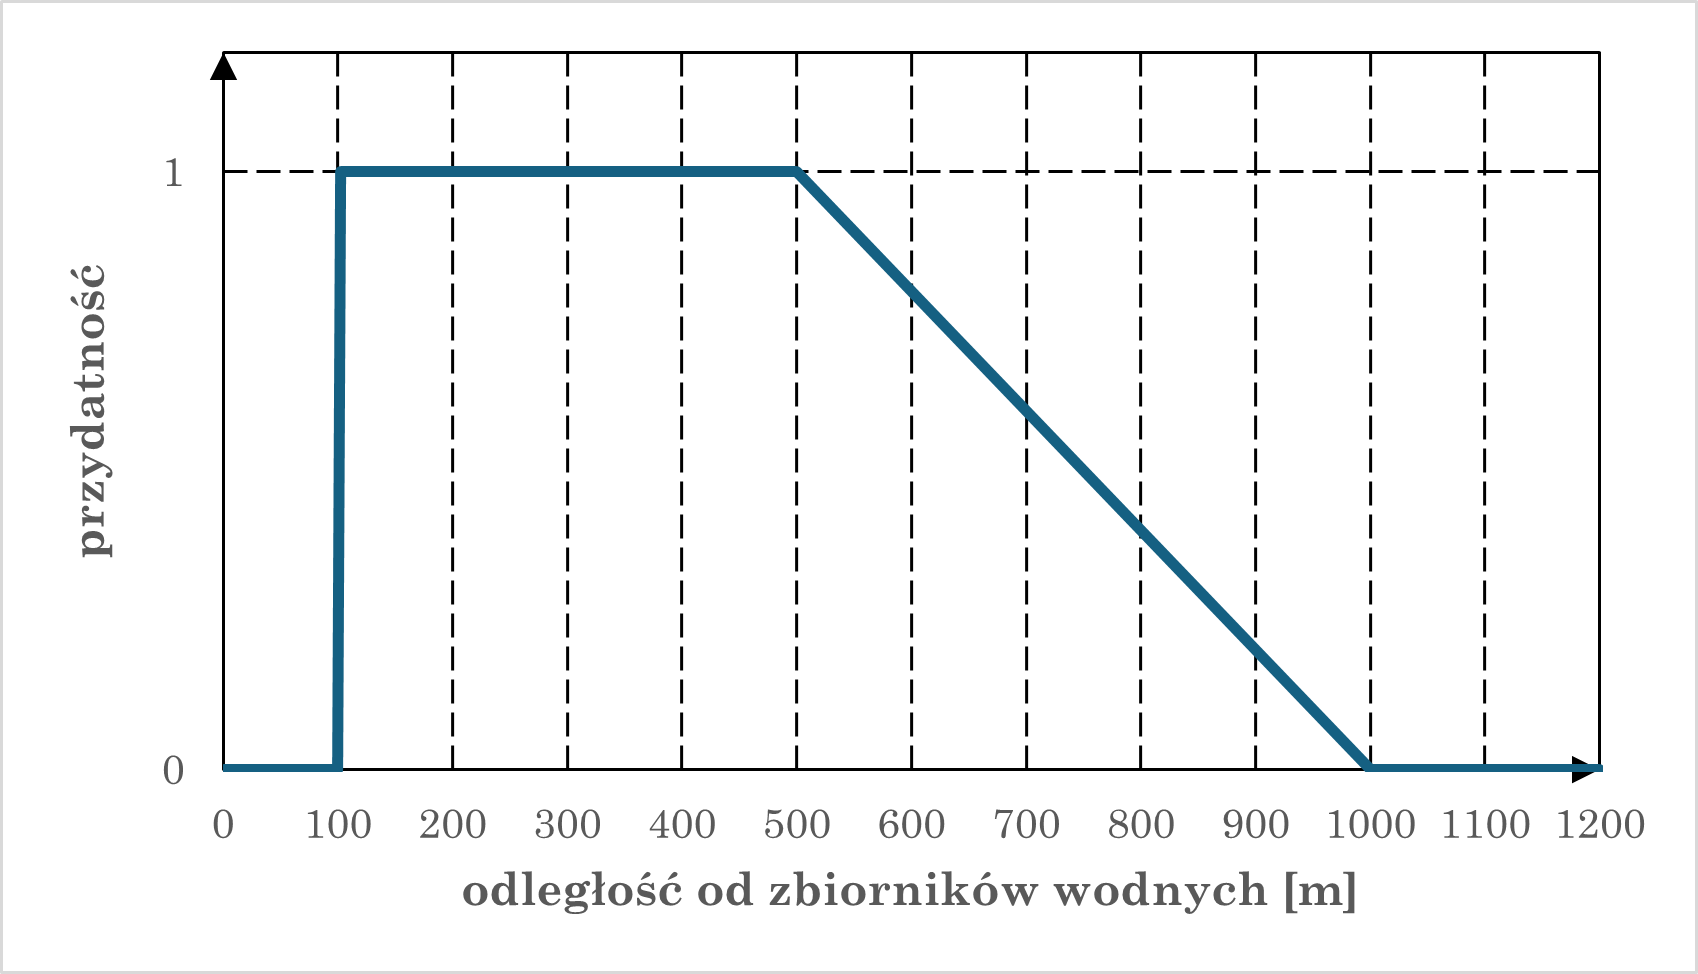
\includegraphics[width=\linewidth]{img/kryterium1-wykres-pierwszy.png}
        \caption*{}
    \end{minipage}
    \begin{minipage}{0.48\textwidth}
        \centering
        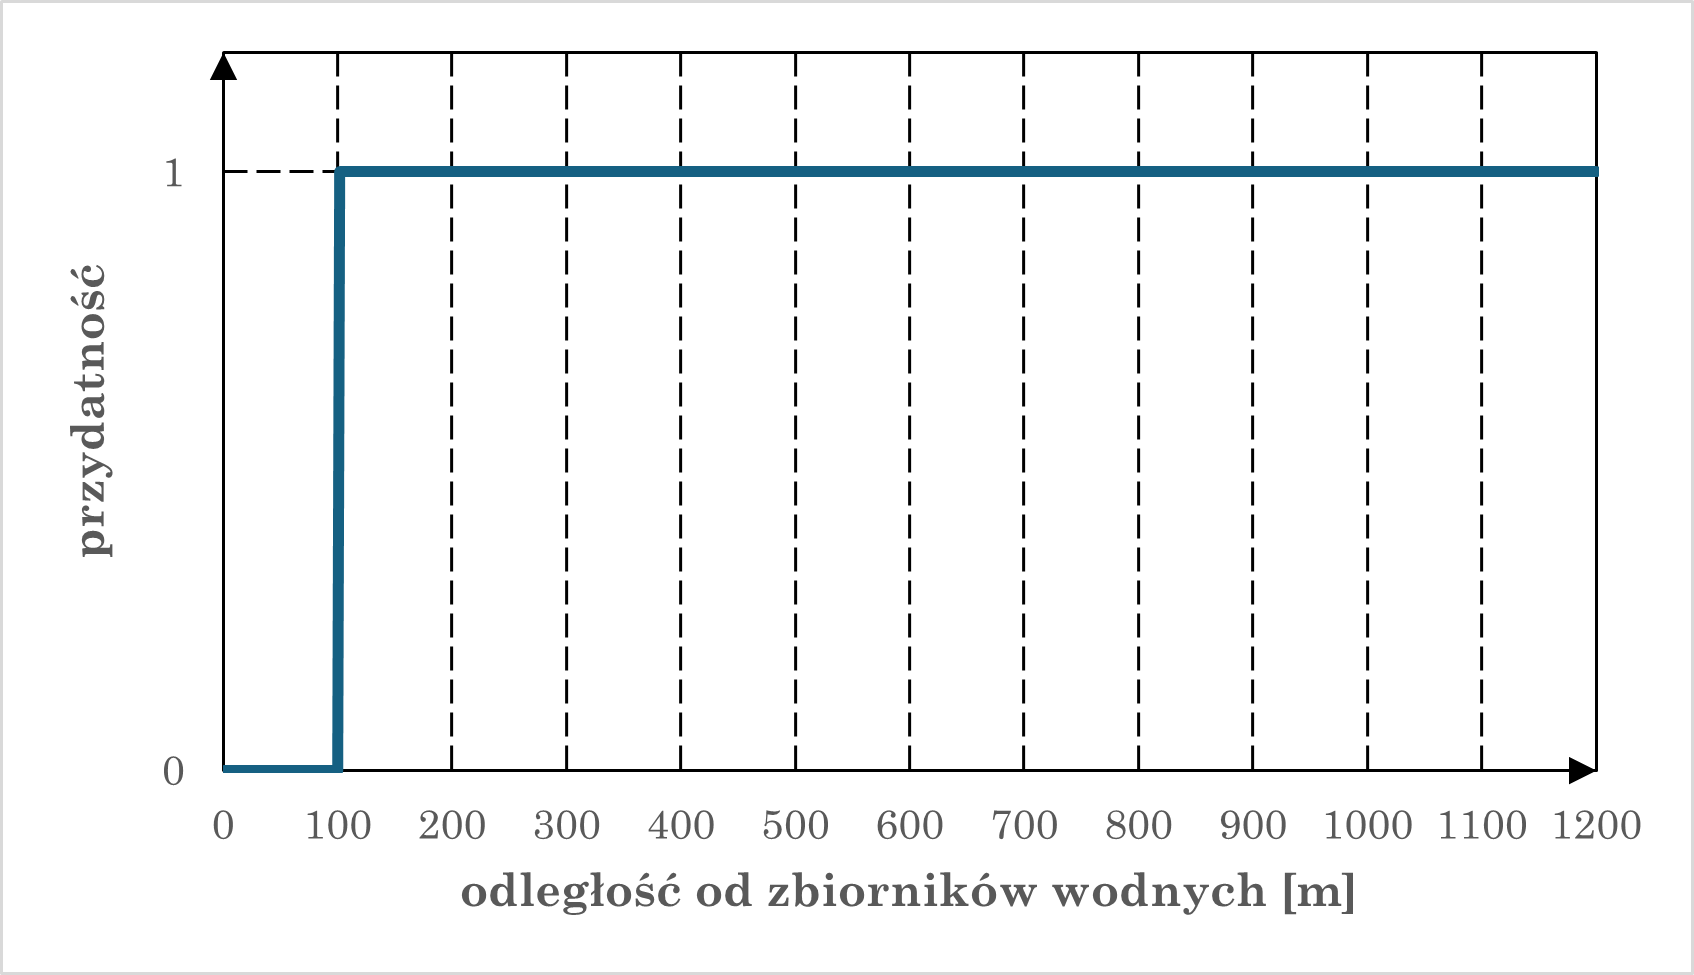
\includegraphics[width=\linewidth]{img/kryterium1-wykres-drugi.png}
        \caption*{}
    \end{minipage}
\end{figure}
\begin{figure}[H]
    \centering
    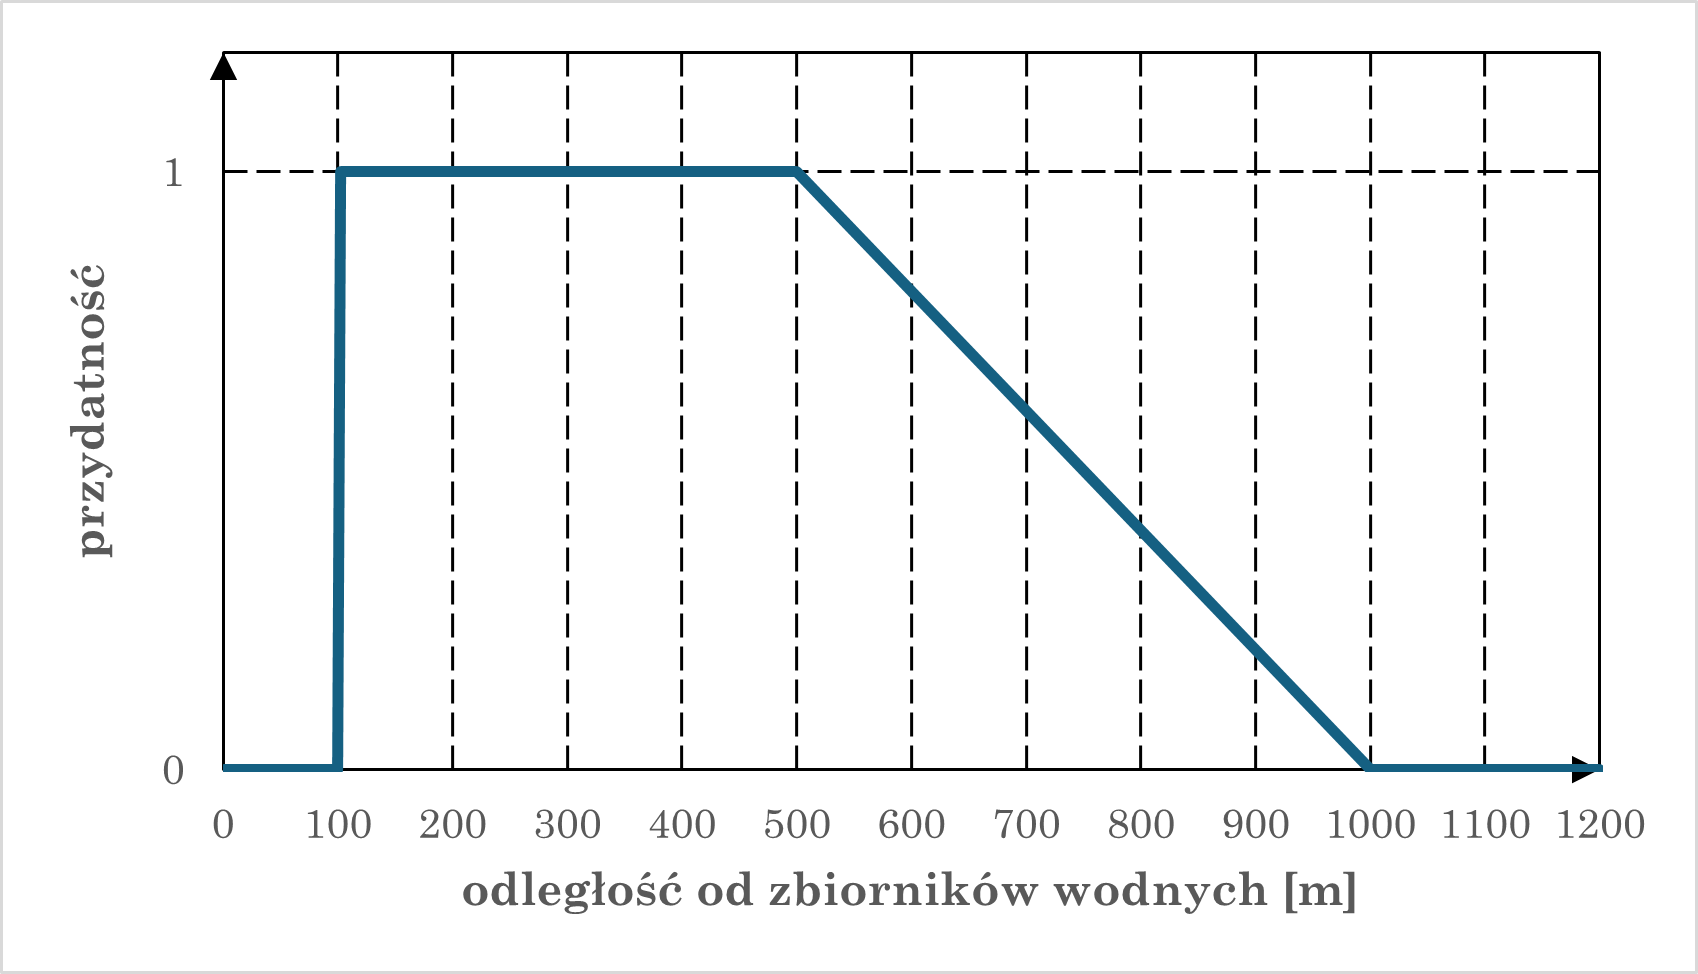
\includegraphics[width=0.75\textwidth]{img/kryterium1-wykres-glowny.png}
    \caption*{Reklasyfikacja dla kryterium 1.}
\end{figure}

\subsubsection{Kod}
\begin{lstlisting}
out_distance_accumulation_raster = arcpy.sa.DistanceAccumulation(in_source_data=water)
woda_rosnaca = arcpy.sa.FuzzyMembership(out_distance_accumulation_raster, fuzzy_function="LINEAR 100 102")
woda_malejaca = arcpy.sa.FuzzyMembership(out_distance_accumulation_raster, fuzzy_function="LINEAR 1000 500")
woda_mapa = arcpy.sa.FuzzyOverlay([woda_rosnaca, woda_malejaca], 'AND')
woda_mapa.save(f'{geobaza}\\kryterium_1')
\end{lstlisting}

\subsubsection{Wynik}
\begin{figure}[H]
    \centering
    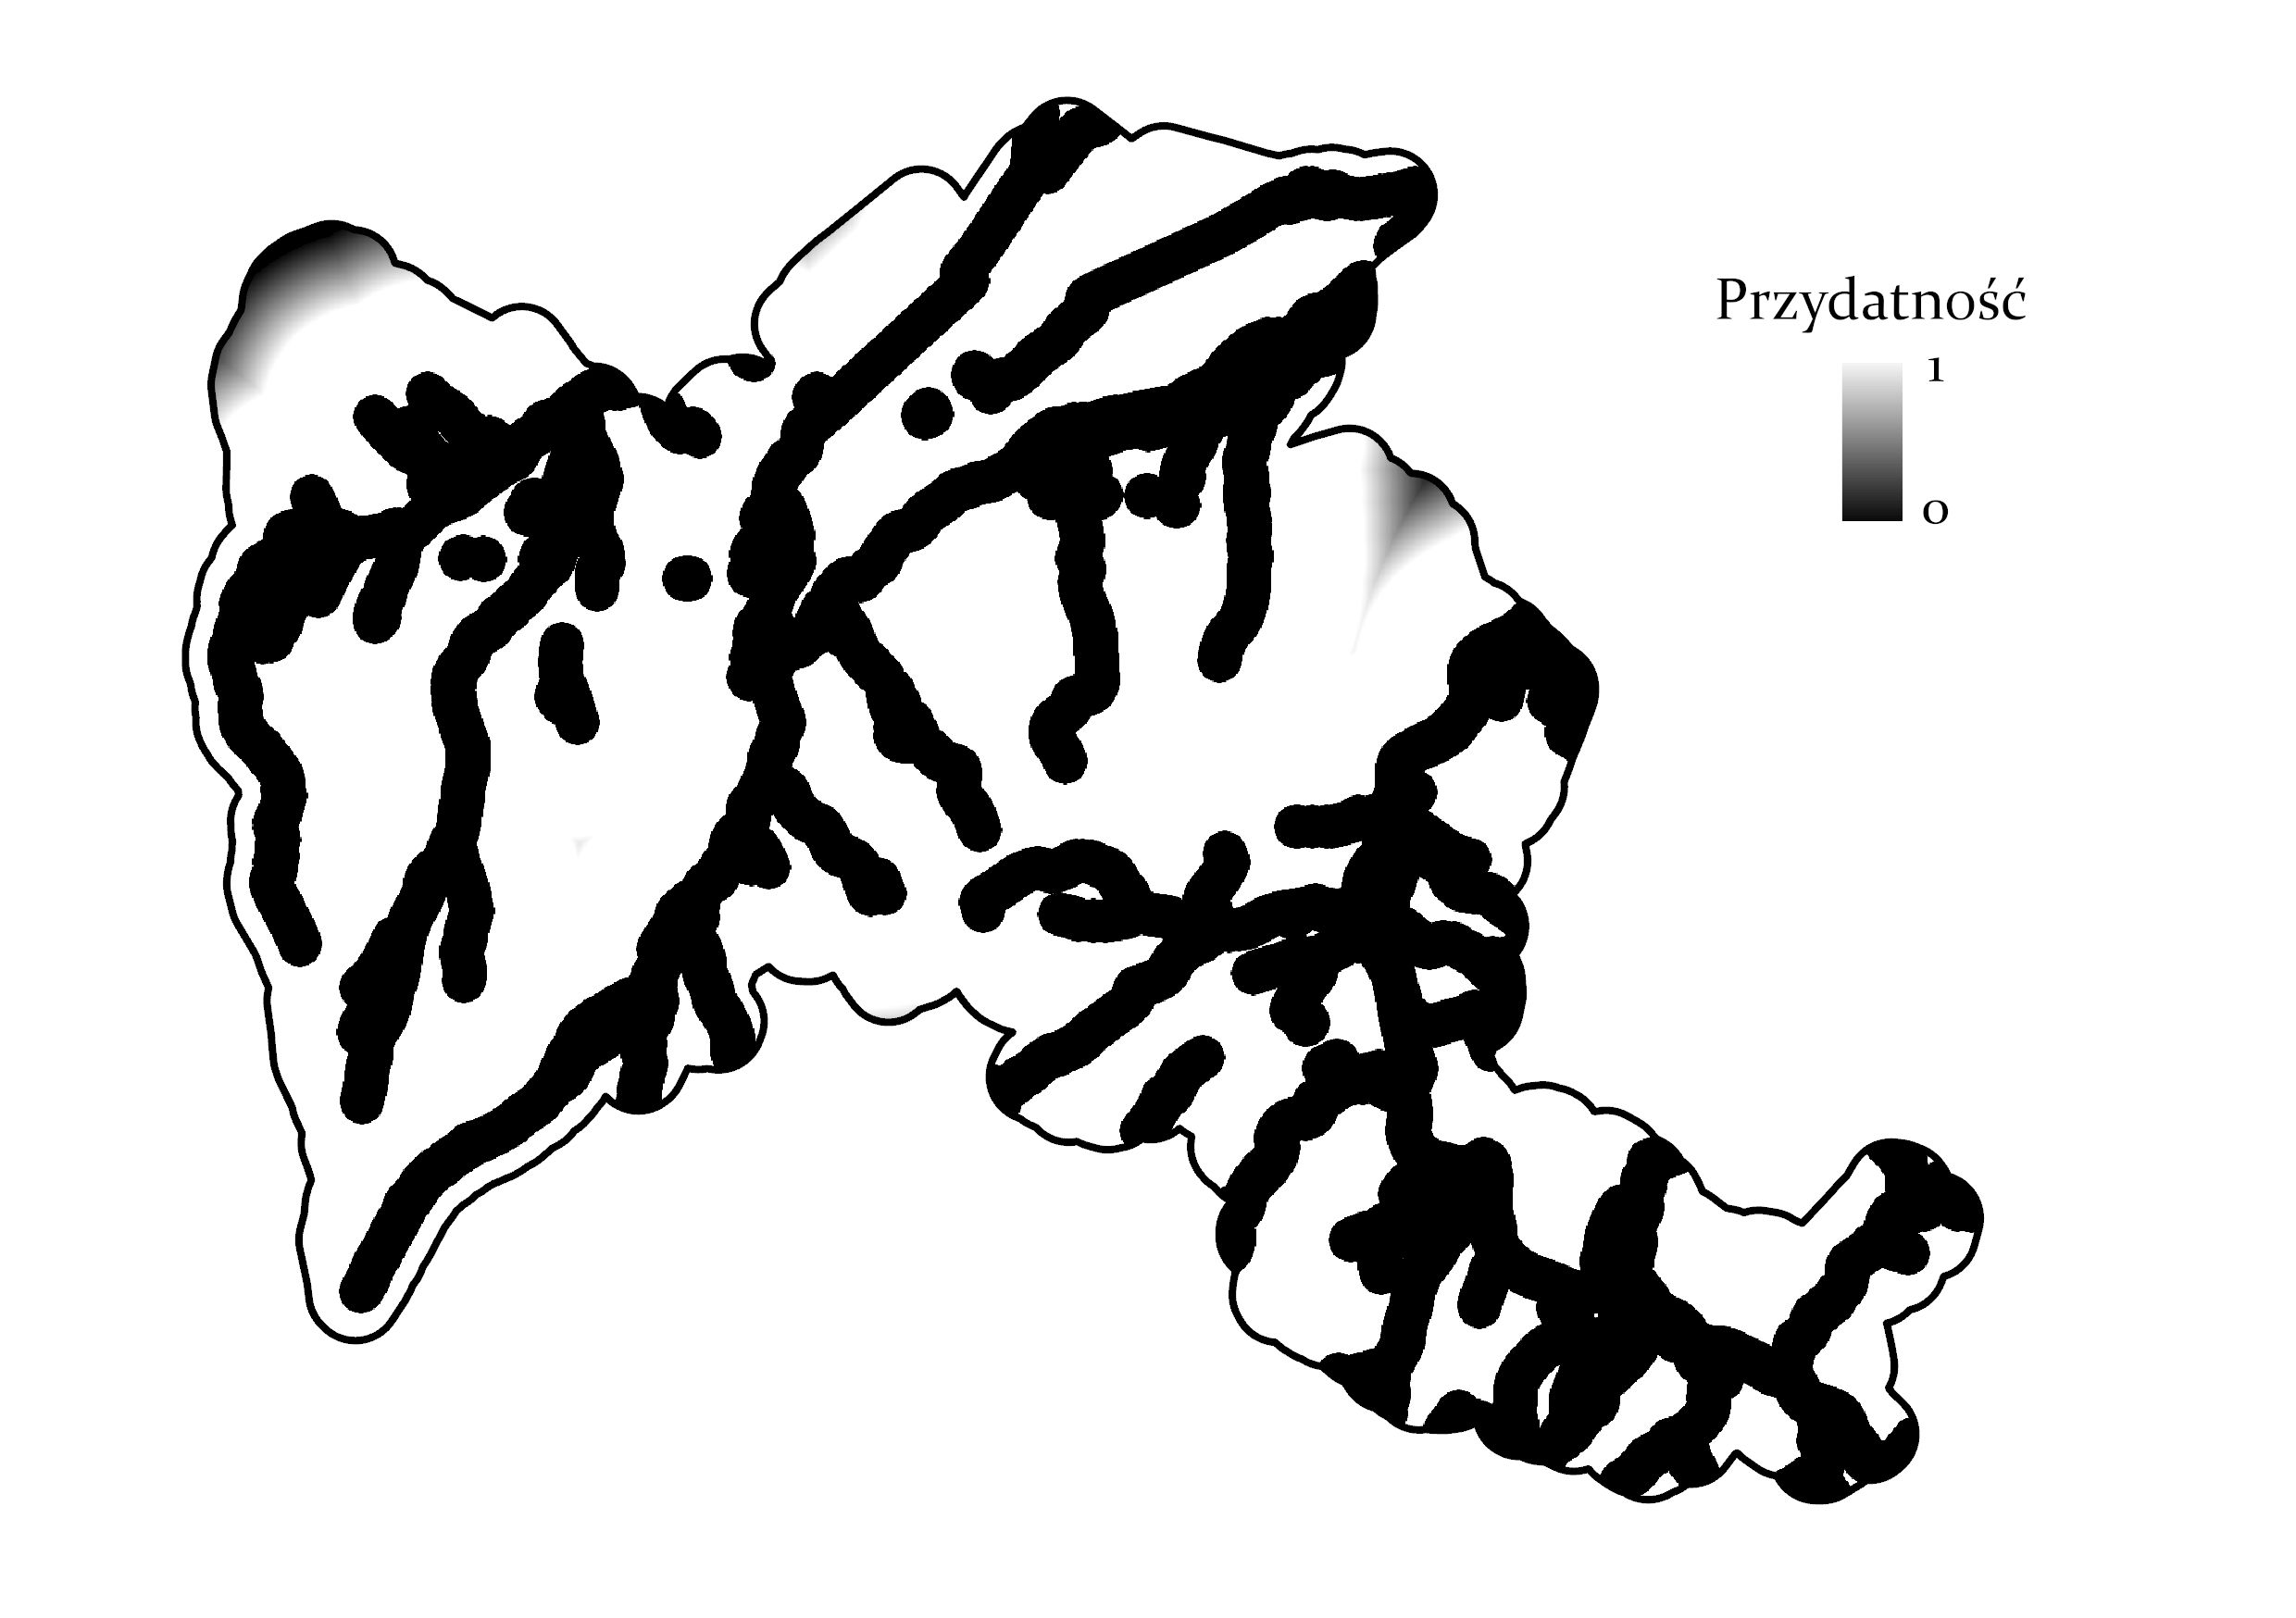
\includegraphics[width=0.75\textwidth]{img/kryterium1-layout.jpg}
    \caption*{Mapa przydatności dla kryterium 1.}
\end{figure}

\begin{figure}[H]
    \centering
    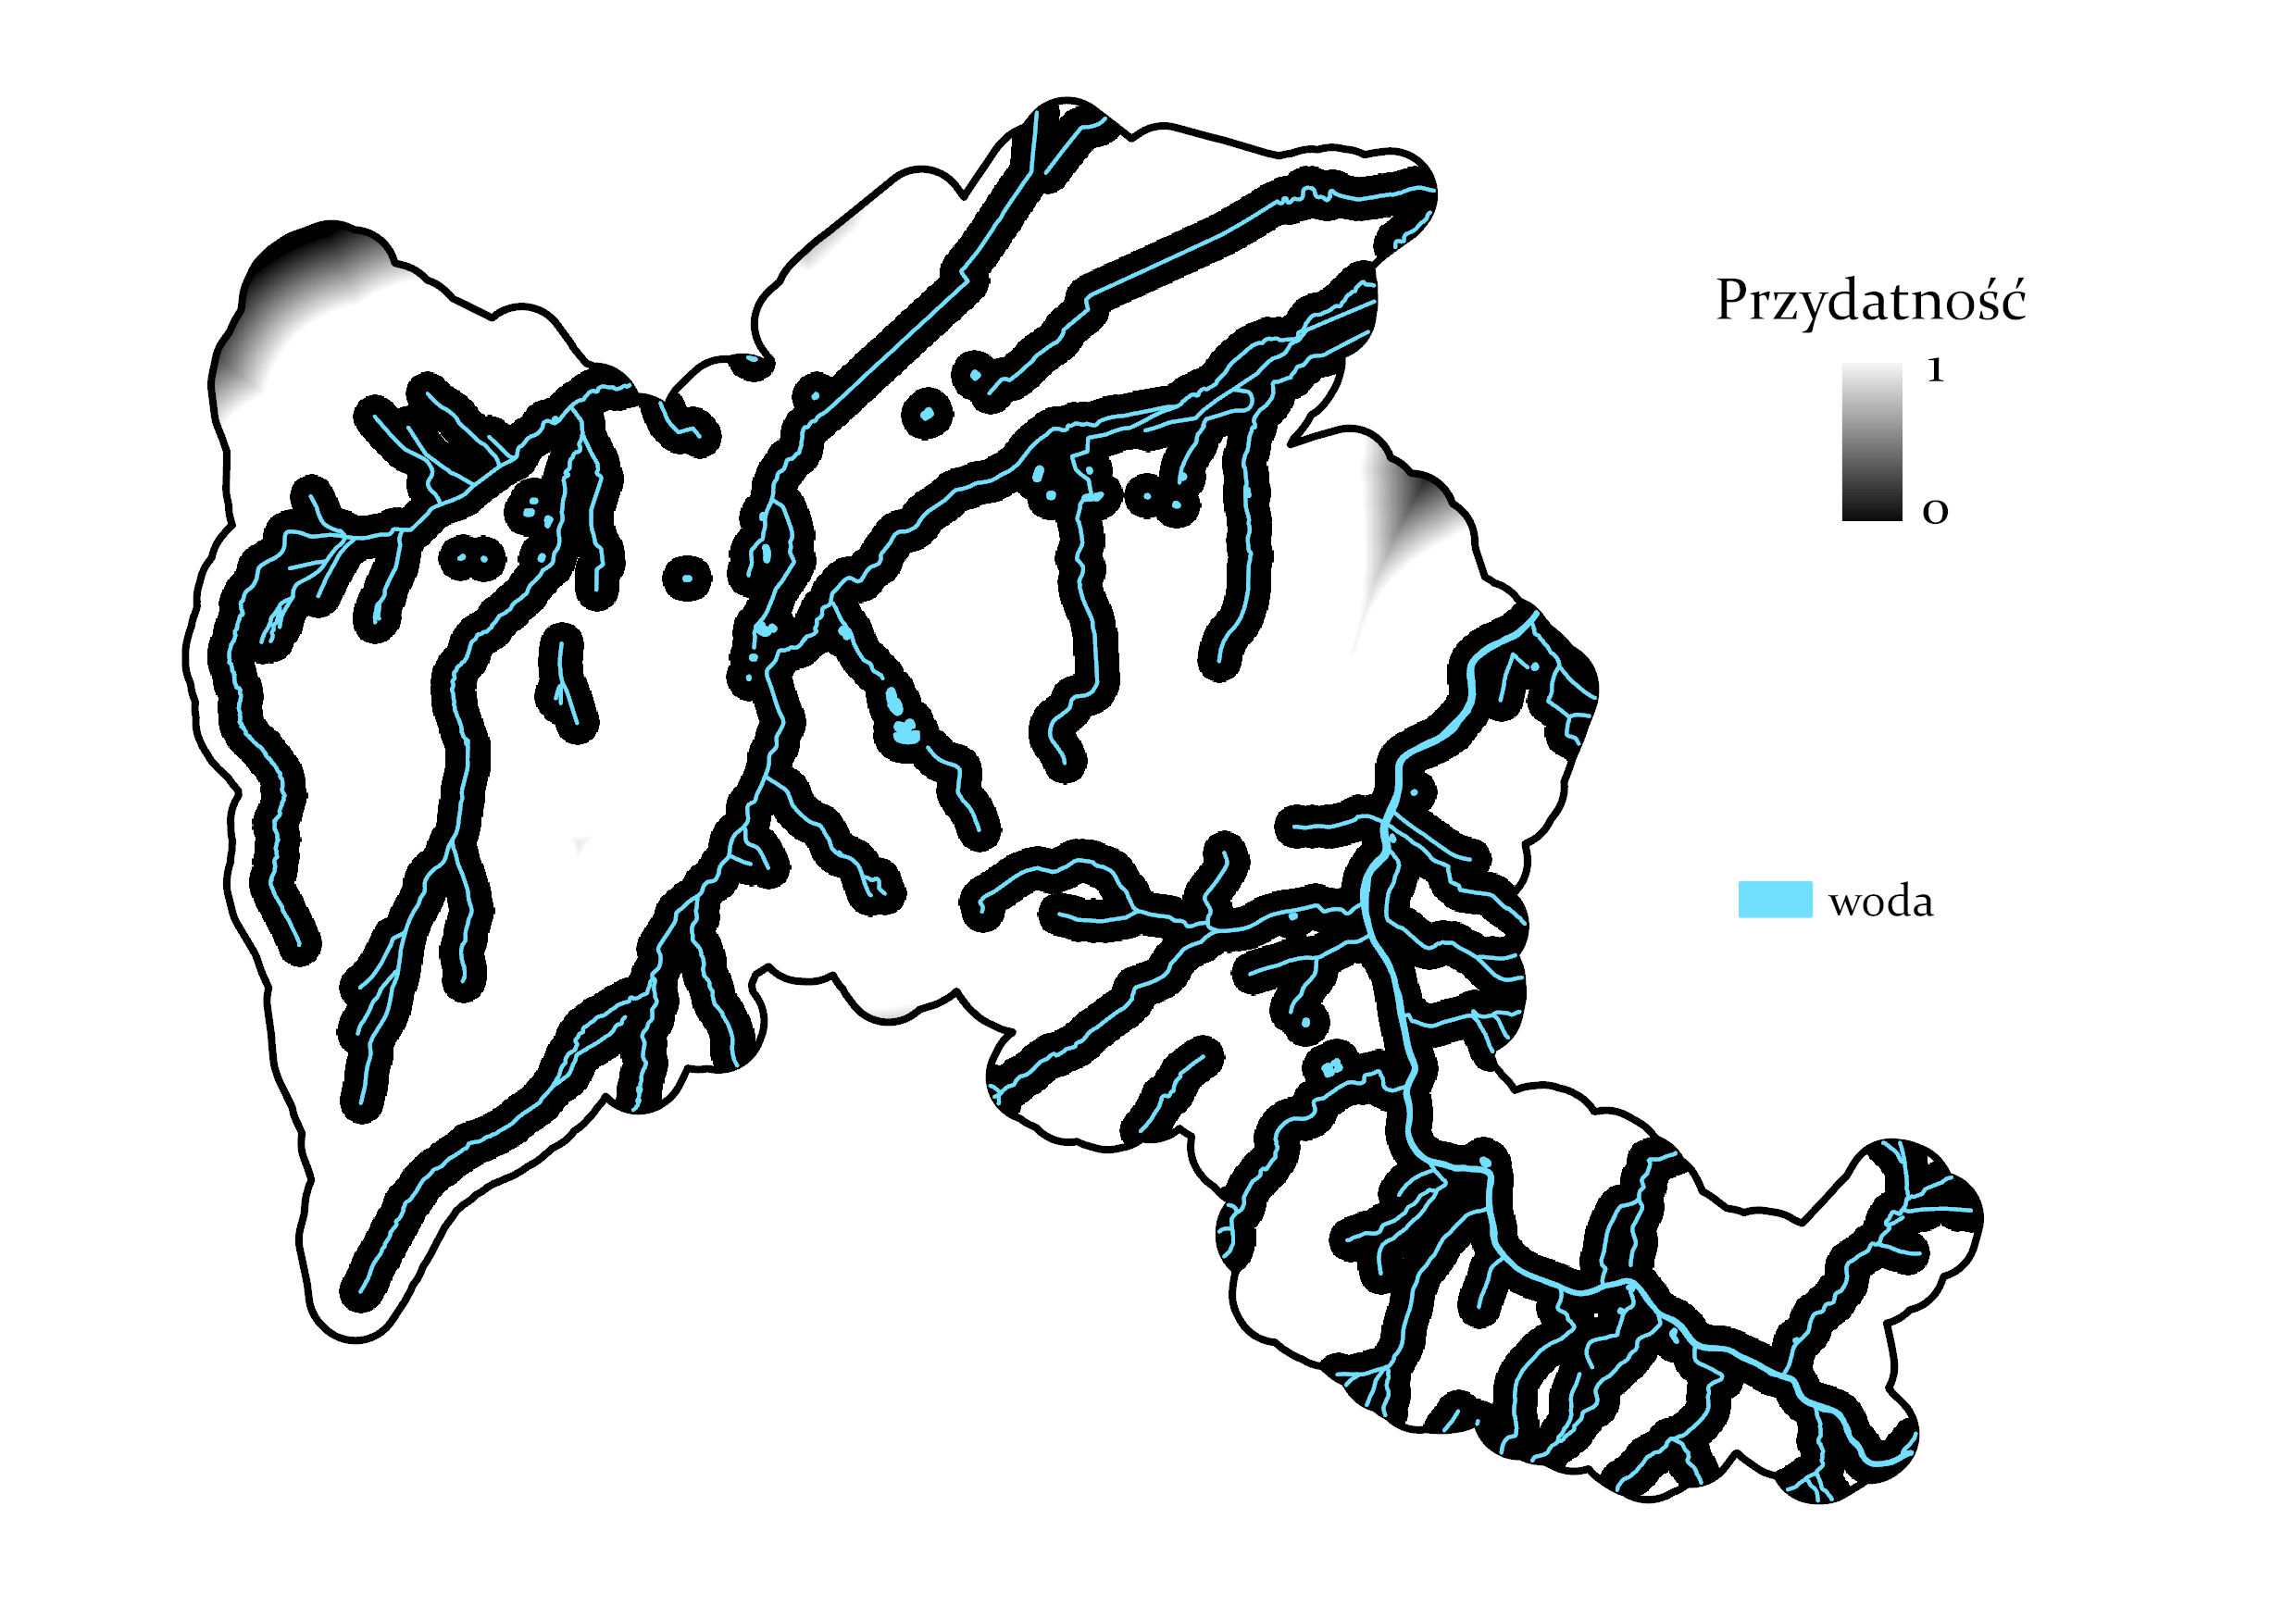
\includegraphics[width=0.75\textwidth]{img/kryterium1-woda.jpg}
    \caption*{Mapa przydatności dla kryterium 1. zawierająca rzeki oraz zbiorniki wodne}
\end{figure}


\newpage
\subsection{Kryterium 2: odległość od budynków mieszkalnych}
\subsubsection{Opis działania}
\begin{figure}[H]
    \centering
    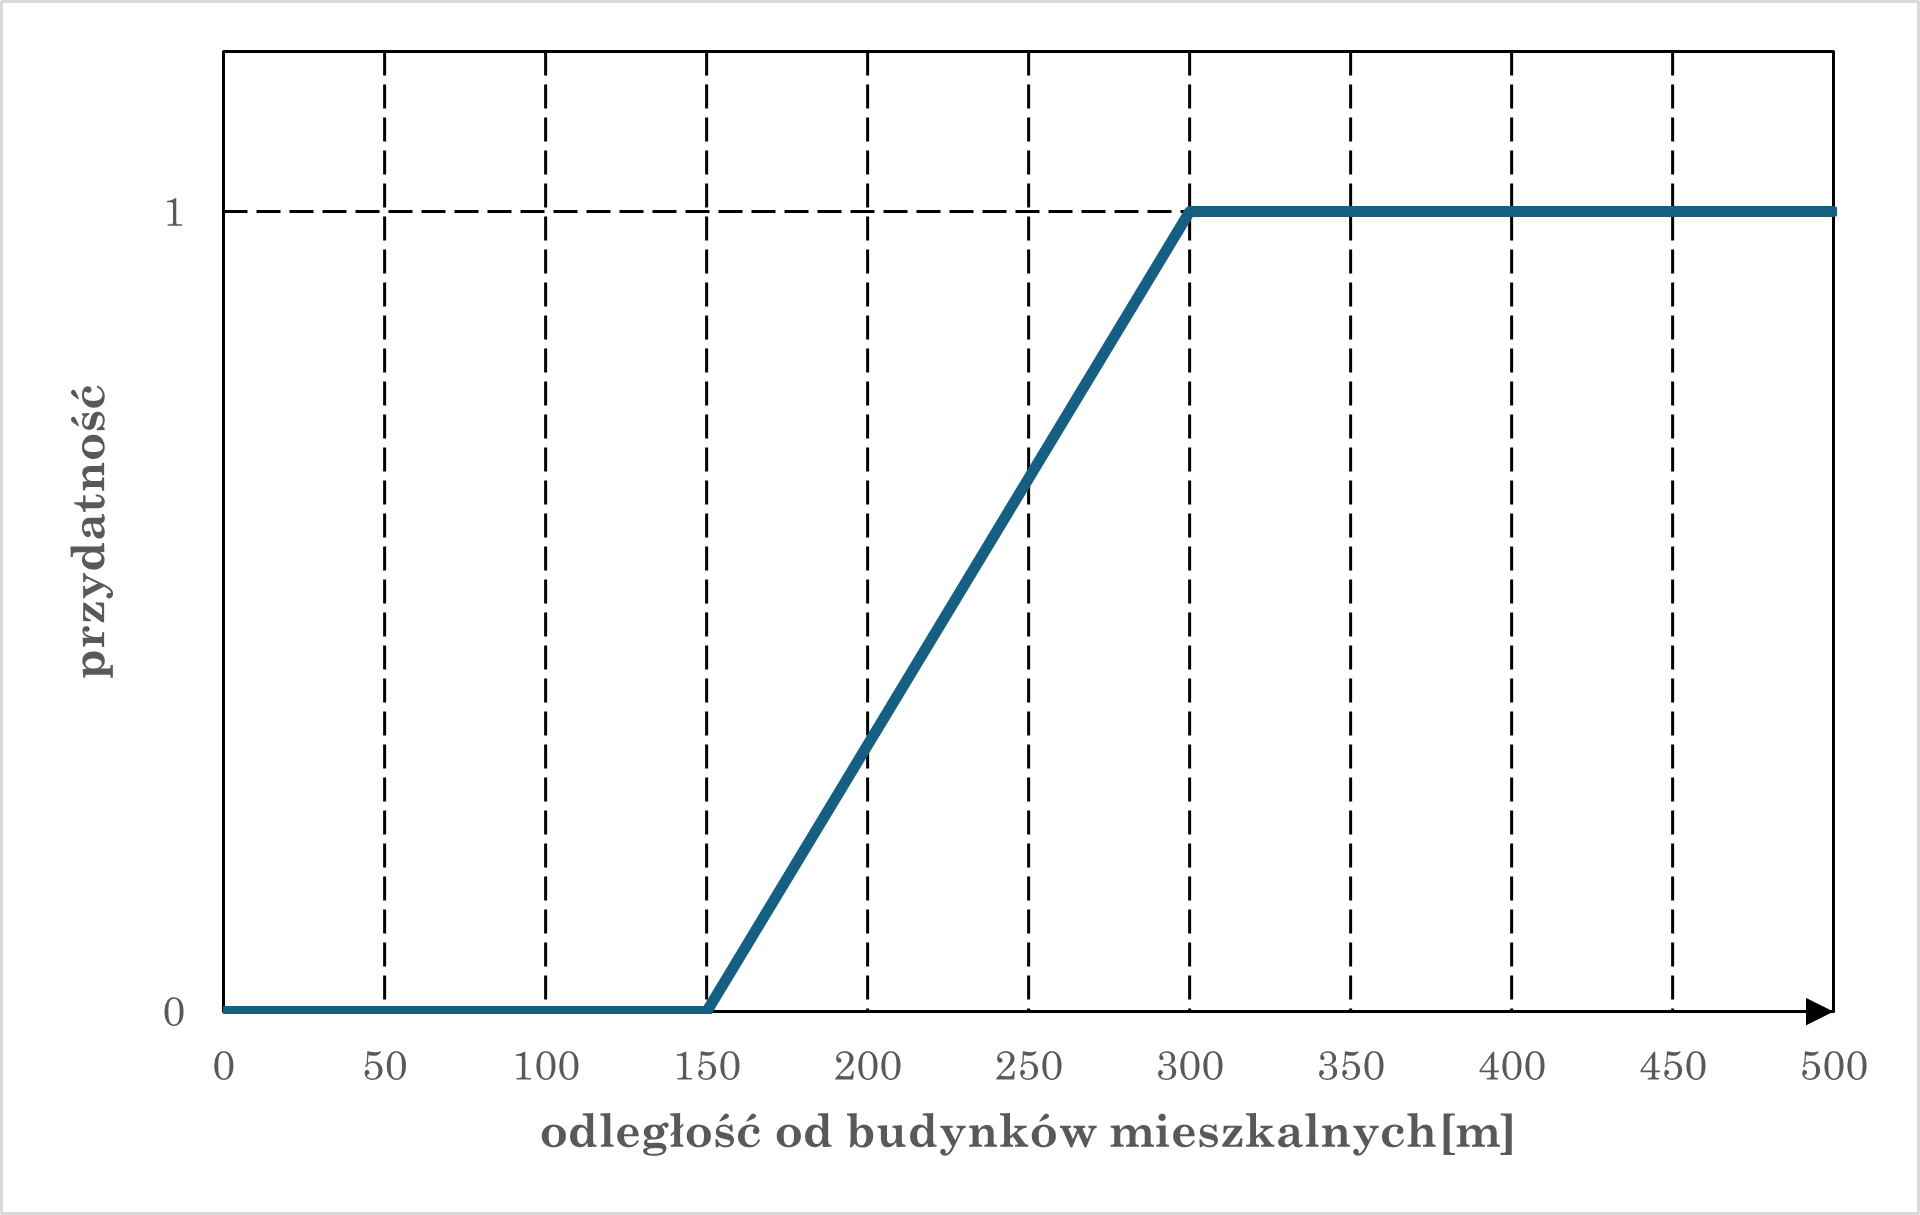
\includegraphics[width=0.75\textwidth]{img/kryterium2-wykres-glowny.png}
    \caption*{Reklasyfikacja dla kryterium 2.}
\end{figure}

\subsubsection{Kod}
\begin{lstlisting}
query = "FOBUD = 'budynki mieszkalne'"
arcpy.analysis.Select(budynki, 'budynki_mieszkalne', query)
out_distance_accumulation_buildings = arcpy.sa.DistanceAccumulation(in_source_data='budynki_mieszkalne')
budynki_mieszkalne = arcpy.sa.FuzzyMembership(out_distance_accumulation_buildings, fuzzy_function="LINEAR 150 300")
budynki_mieszkalne.save(f'{geobaza}\\kryterium_2')
\end{lstlisting}

\subsubsection{Wynik}
\begin{figure}[H]
    \centering
    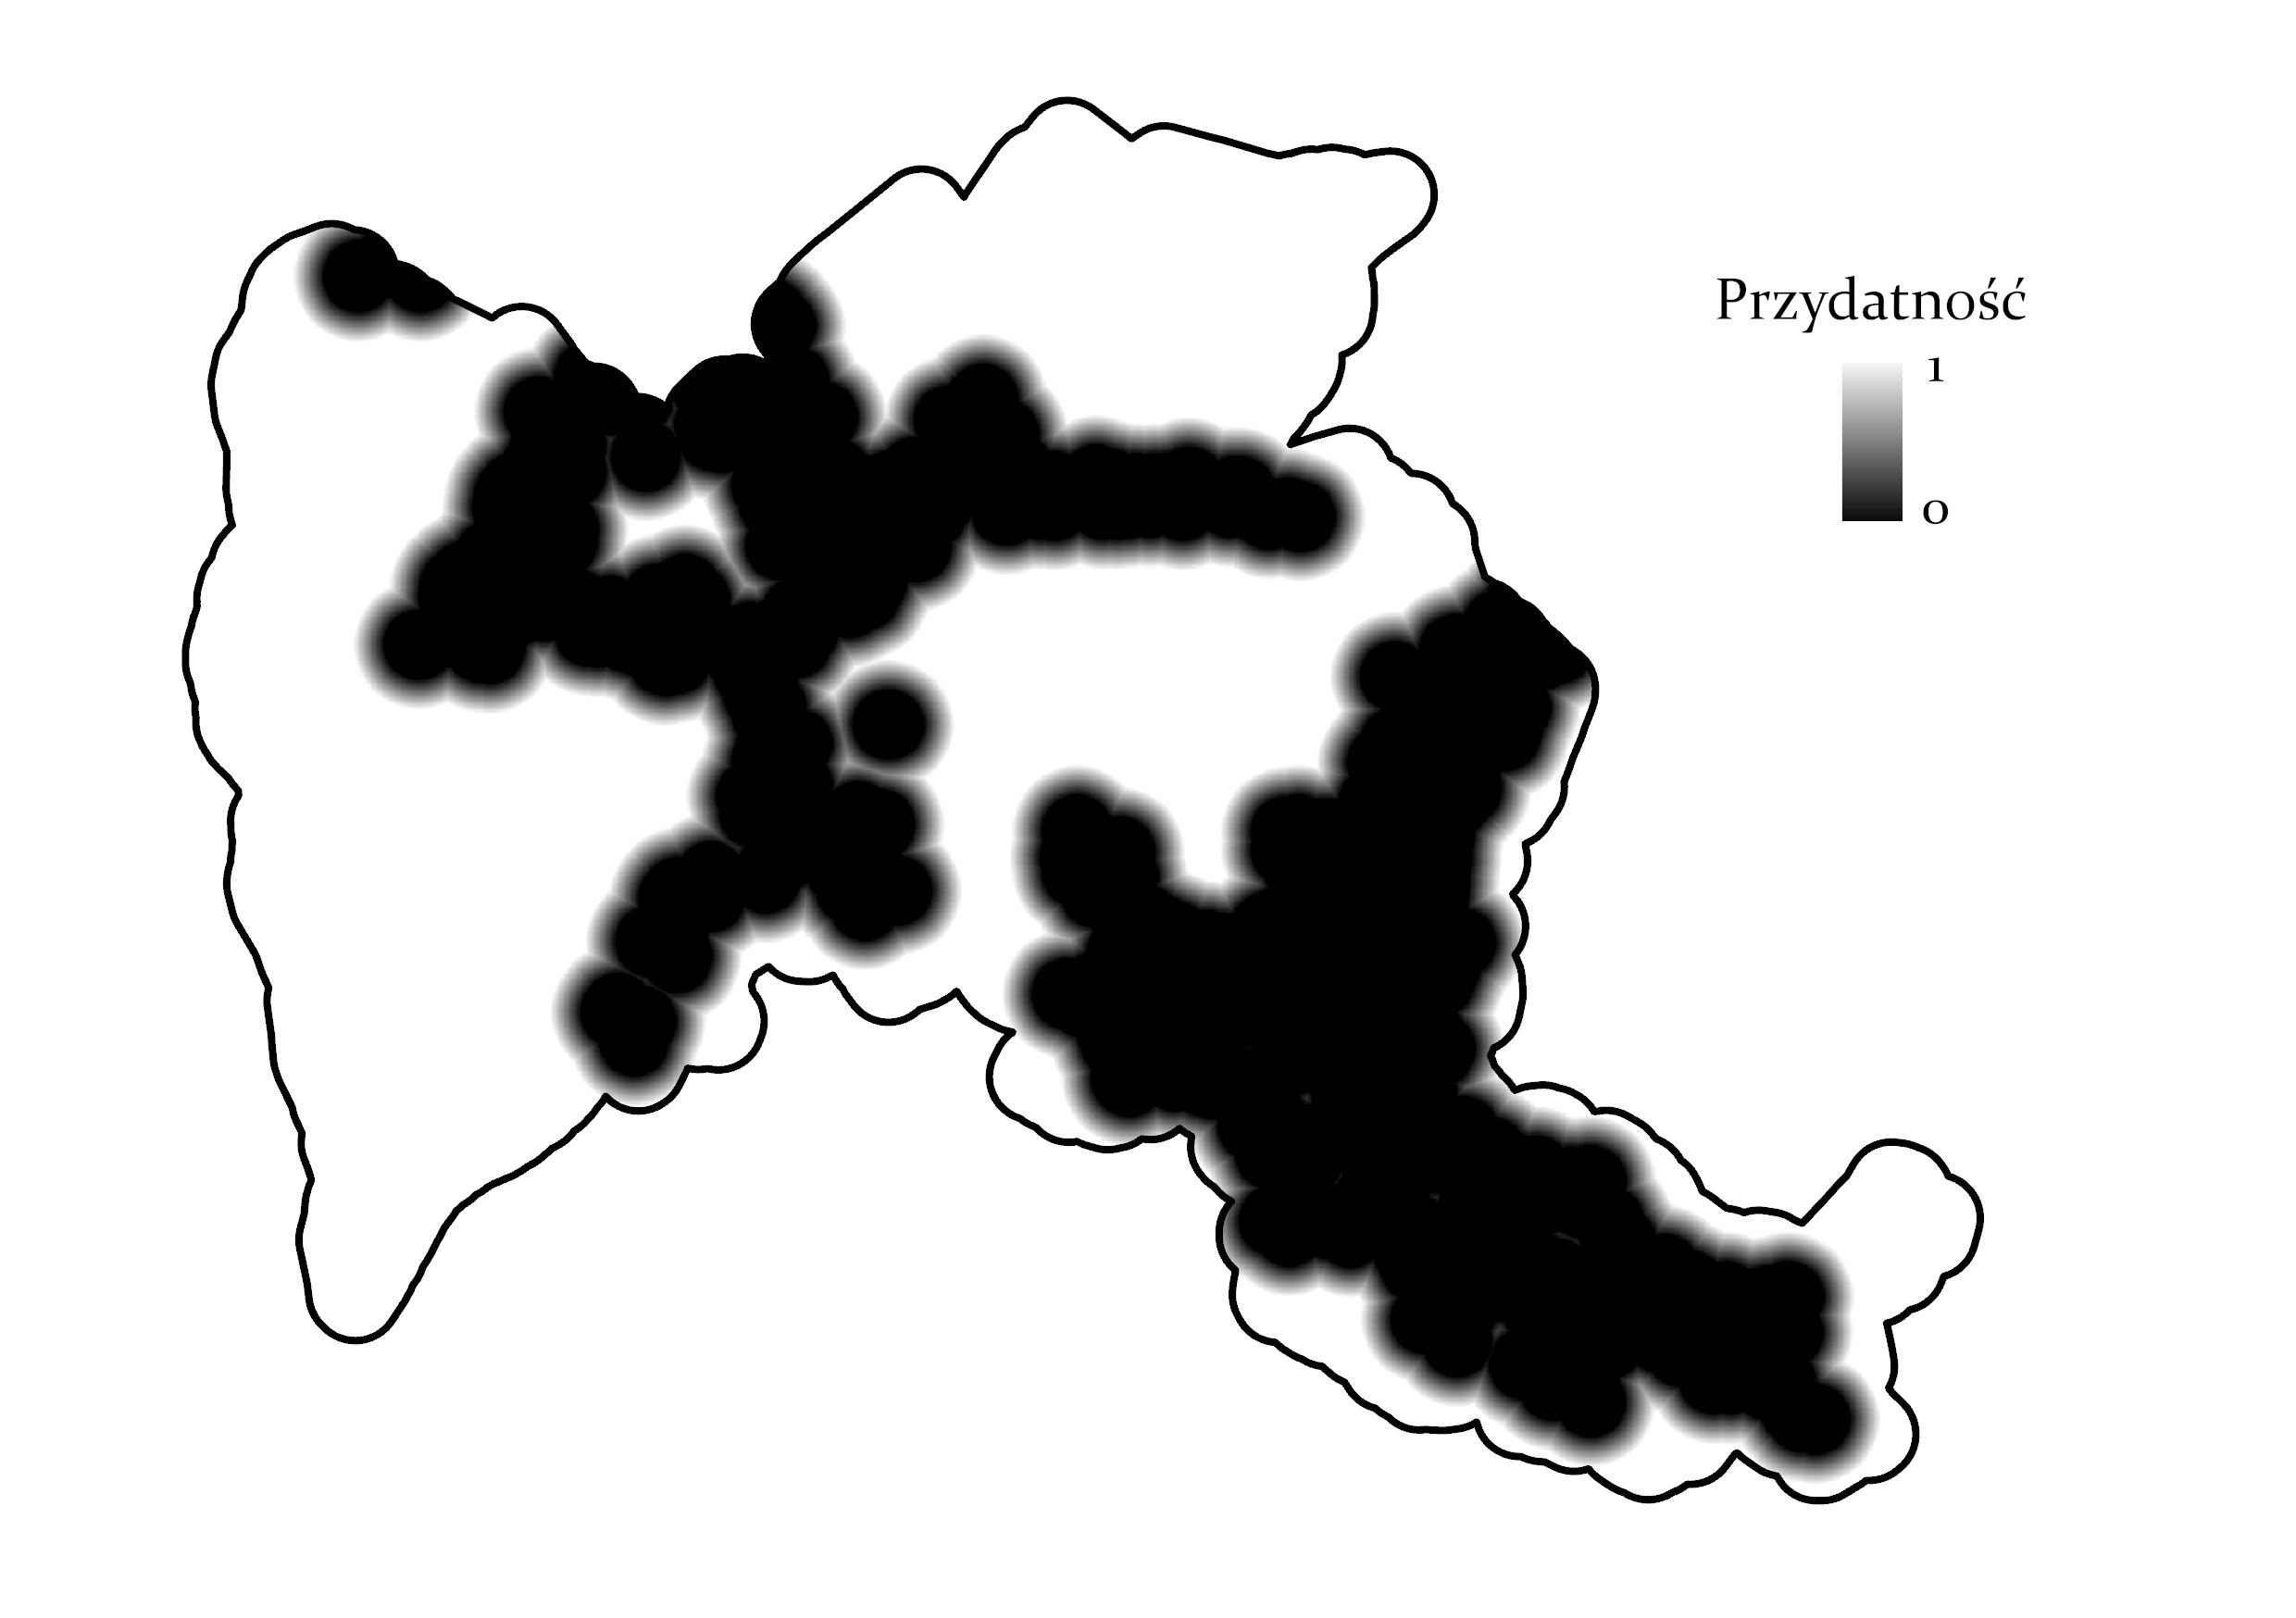
\includegraphics[width=0.75\textwidth]{img/kryterium2-layout.jpg}
    \caption*{Mapa przydatności dla kryterium 2.}
\end{figure}

\begin{figure}[H]
    \centering
    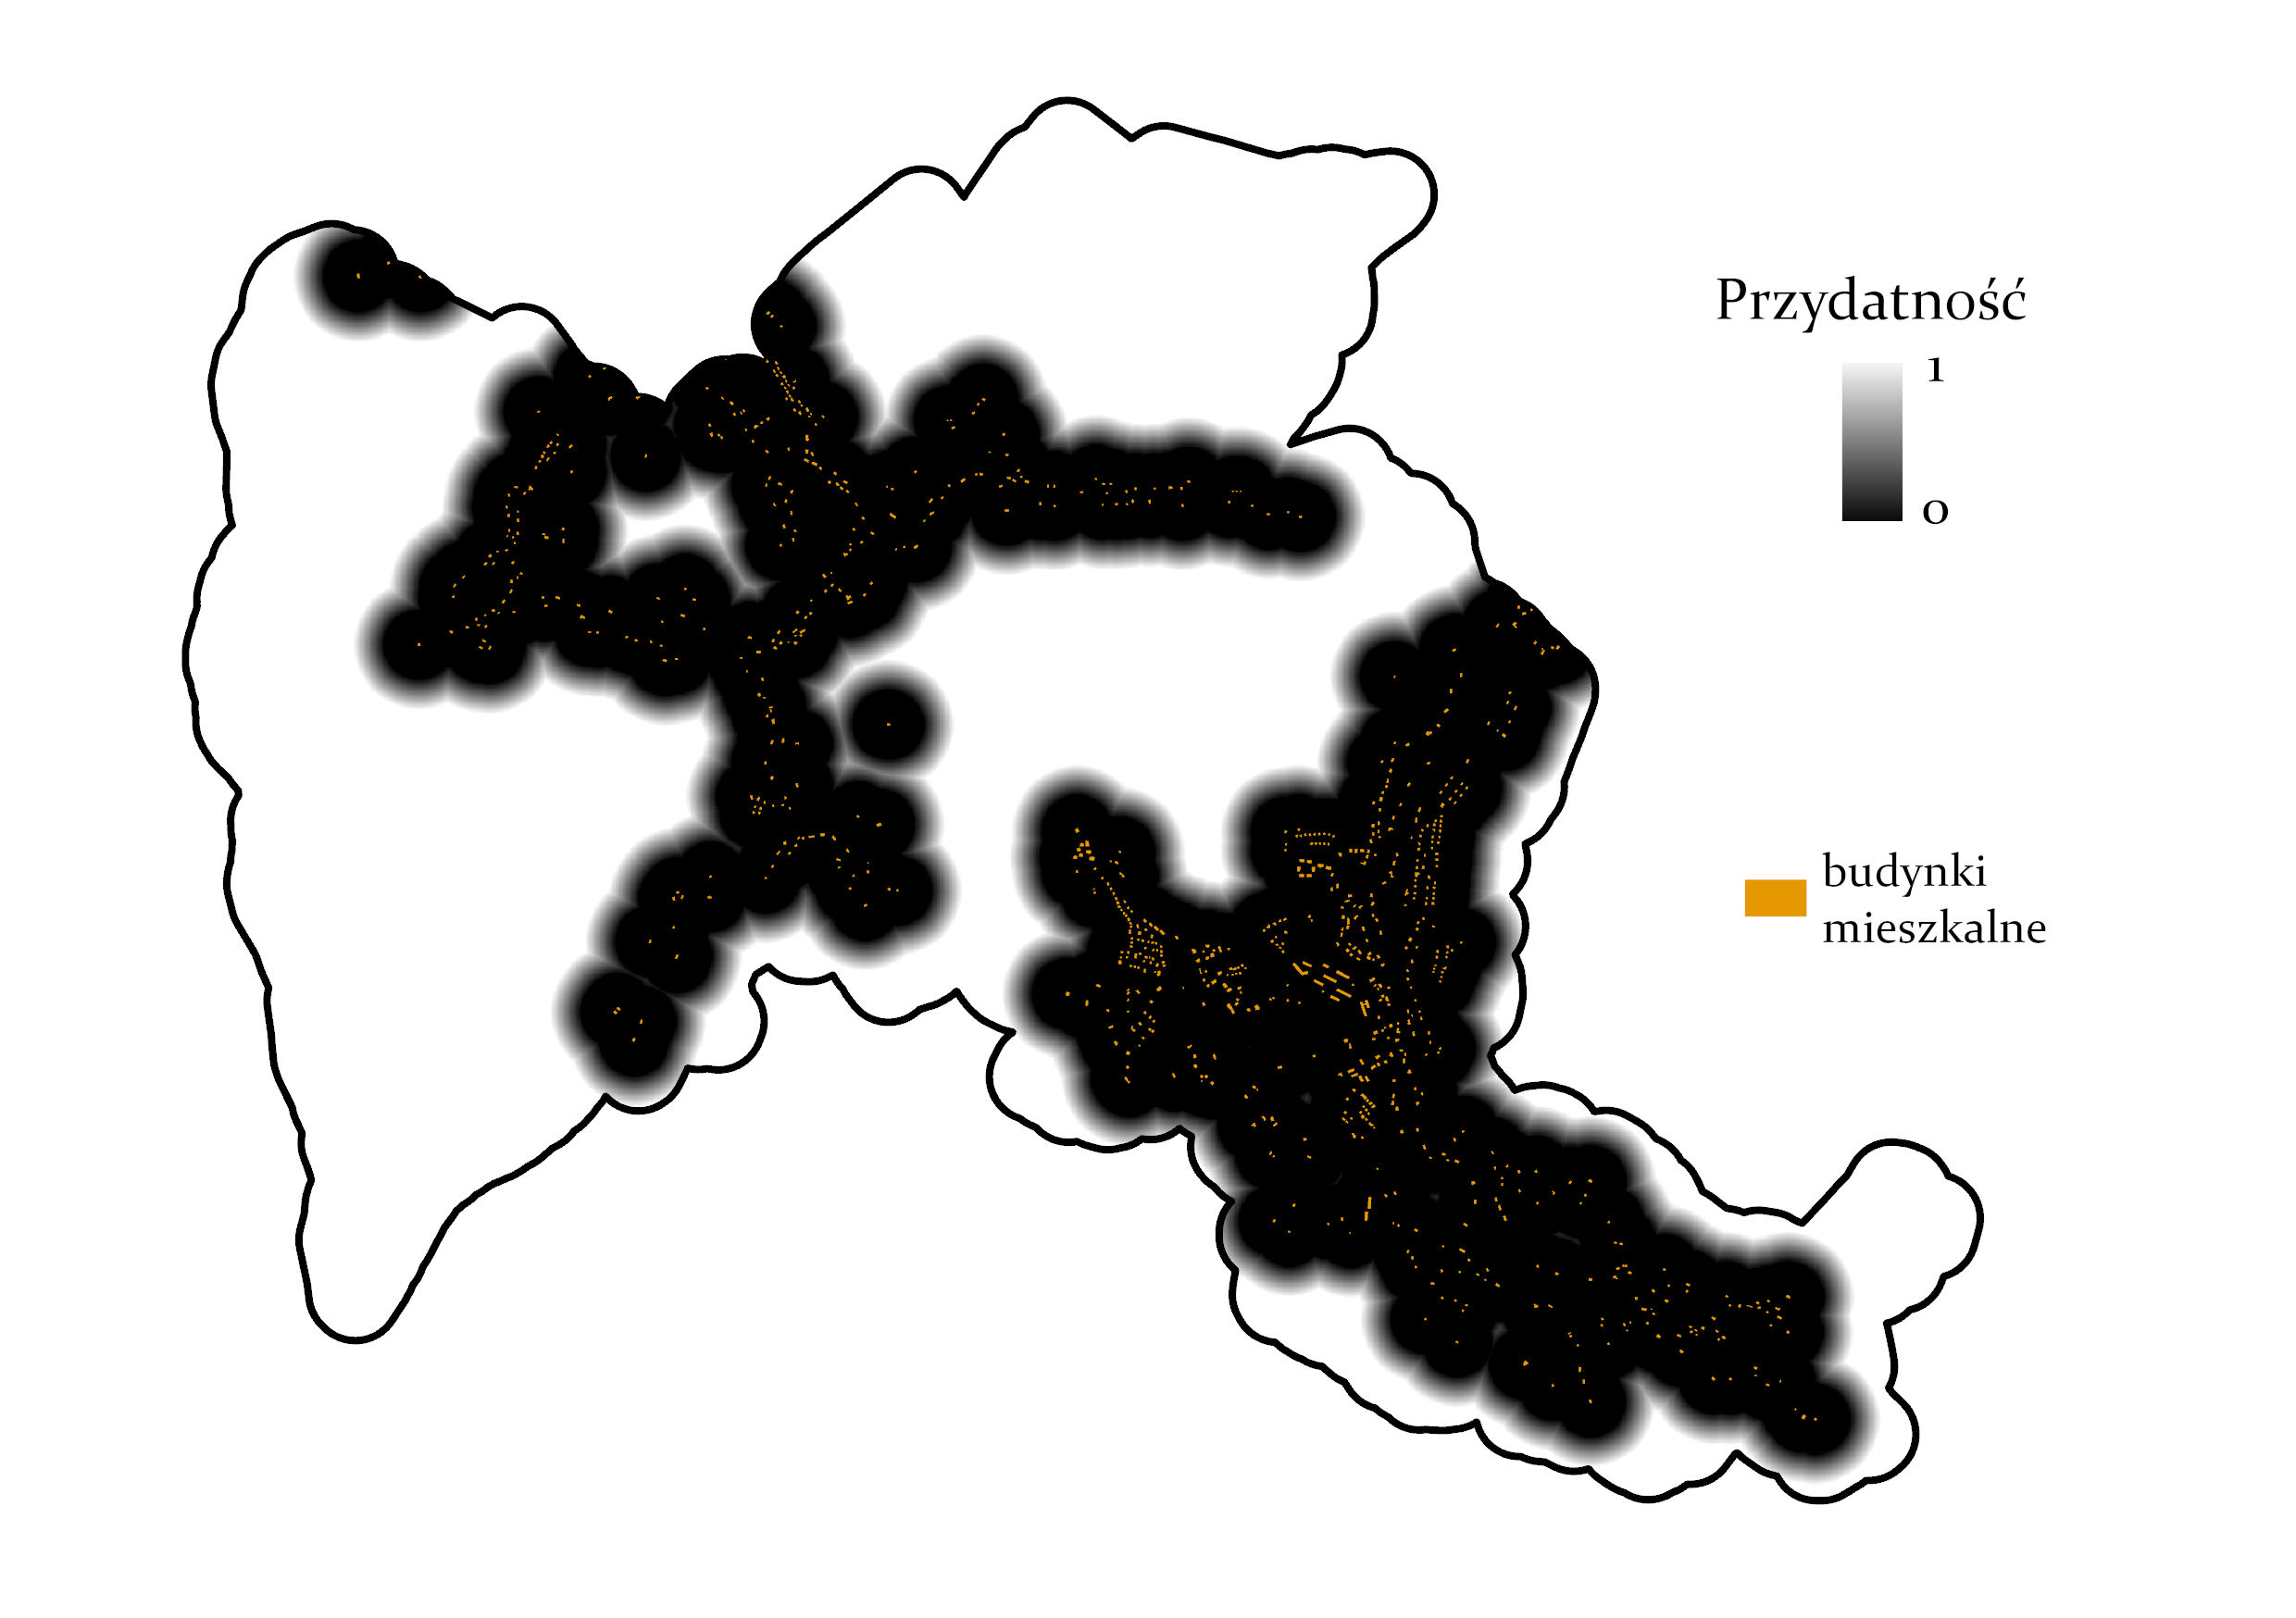
\includegraphics[width=0.75\textwidth]{img/kryterium2-budynki.jpg}
    \caption*{Mapa przydatności dla kryterium 2. zawierająca budynki mieszkalne}
\end{figure}


\newpage
\subsection{Kryterium 3: pokrycie terenu}
\subsubsection{Opis działania}
\begin{figure}[H]
    \centering
    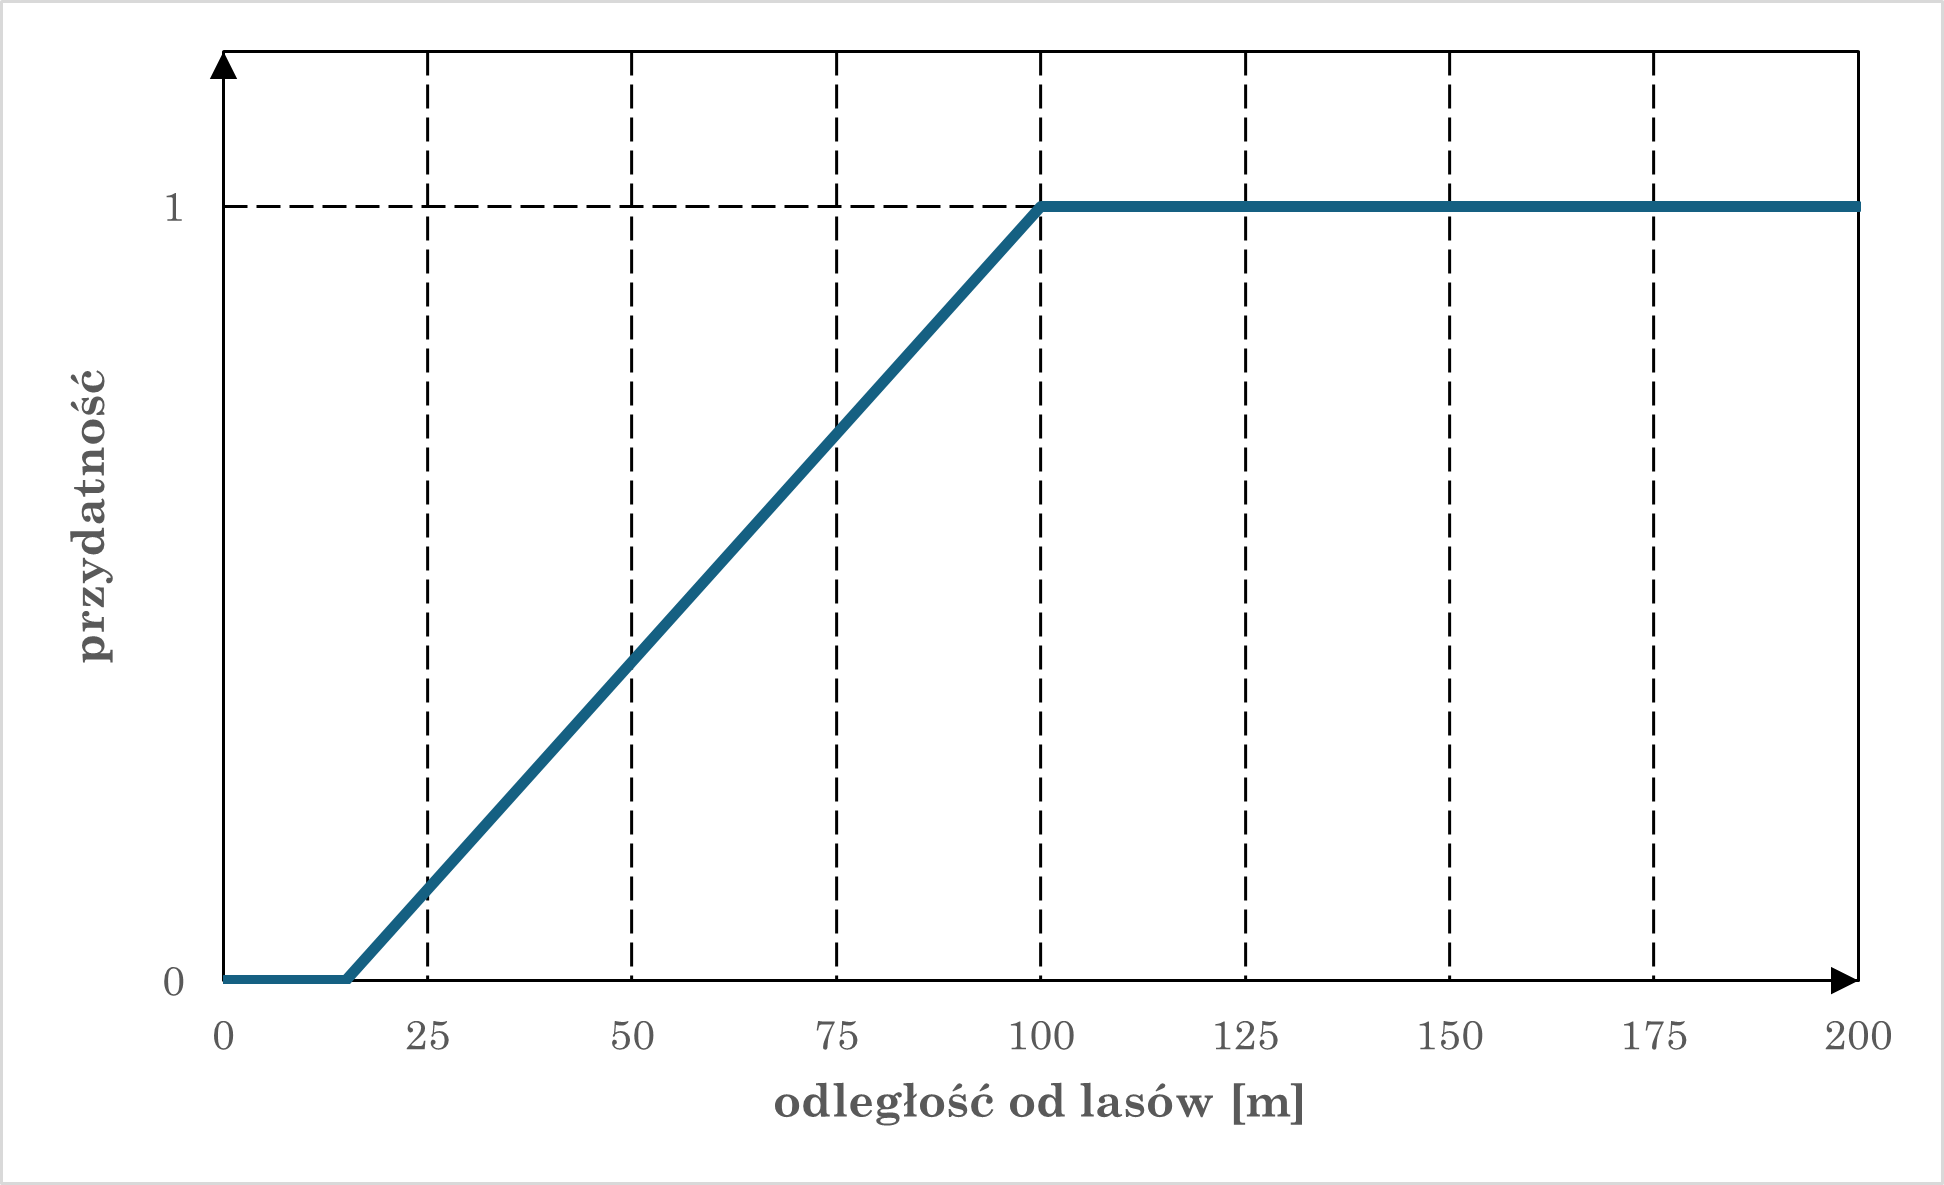
\includegraphics[width=0.75\textwidth]{img/kryterium3-wykres-glowny.png}
    \caption*{Reklasyfikacja dla kryterium 3.}
\end{figure}

\subsubsection{Kod}
\begin{lstlisting}
query = "RODZAJ = 'las'"
arcpy.analysis.Select(ptlz, 'ptlz_las', query)
out_distance_accumulation_ptlz = arcpy.sa.DistanceAccumulation(in_source_data="ptlz_las")
lasy_fuzzy = arcpy.sa.FuzzyMembership(out_distance_accumulation_ptlz, fuzzy_function="LINEAR 15 100")
lasy_fuzzy.save(f'{geobaza}\\kryterium_3')
\end{lstlisting}

\subsubsection{Wynik}
\begin{figure}[H]
    \centering
    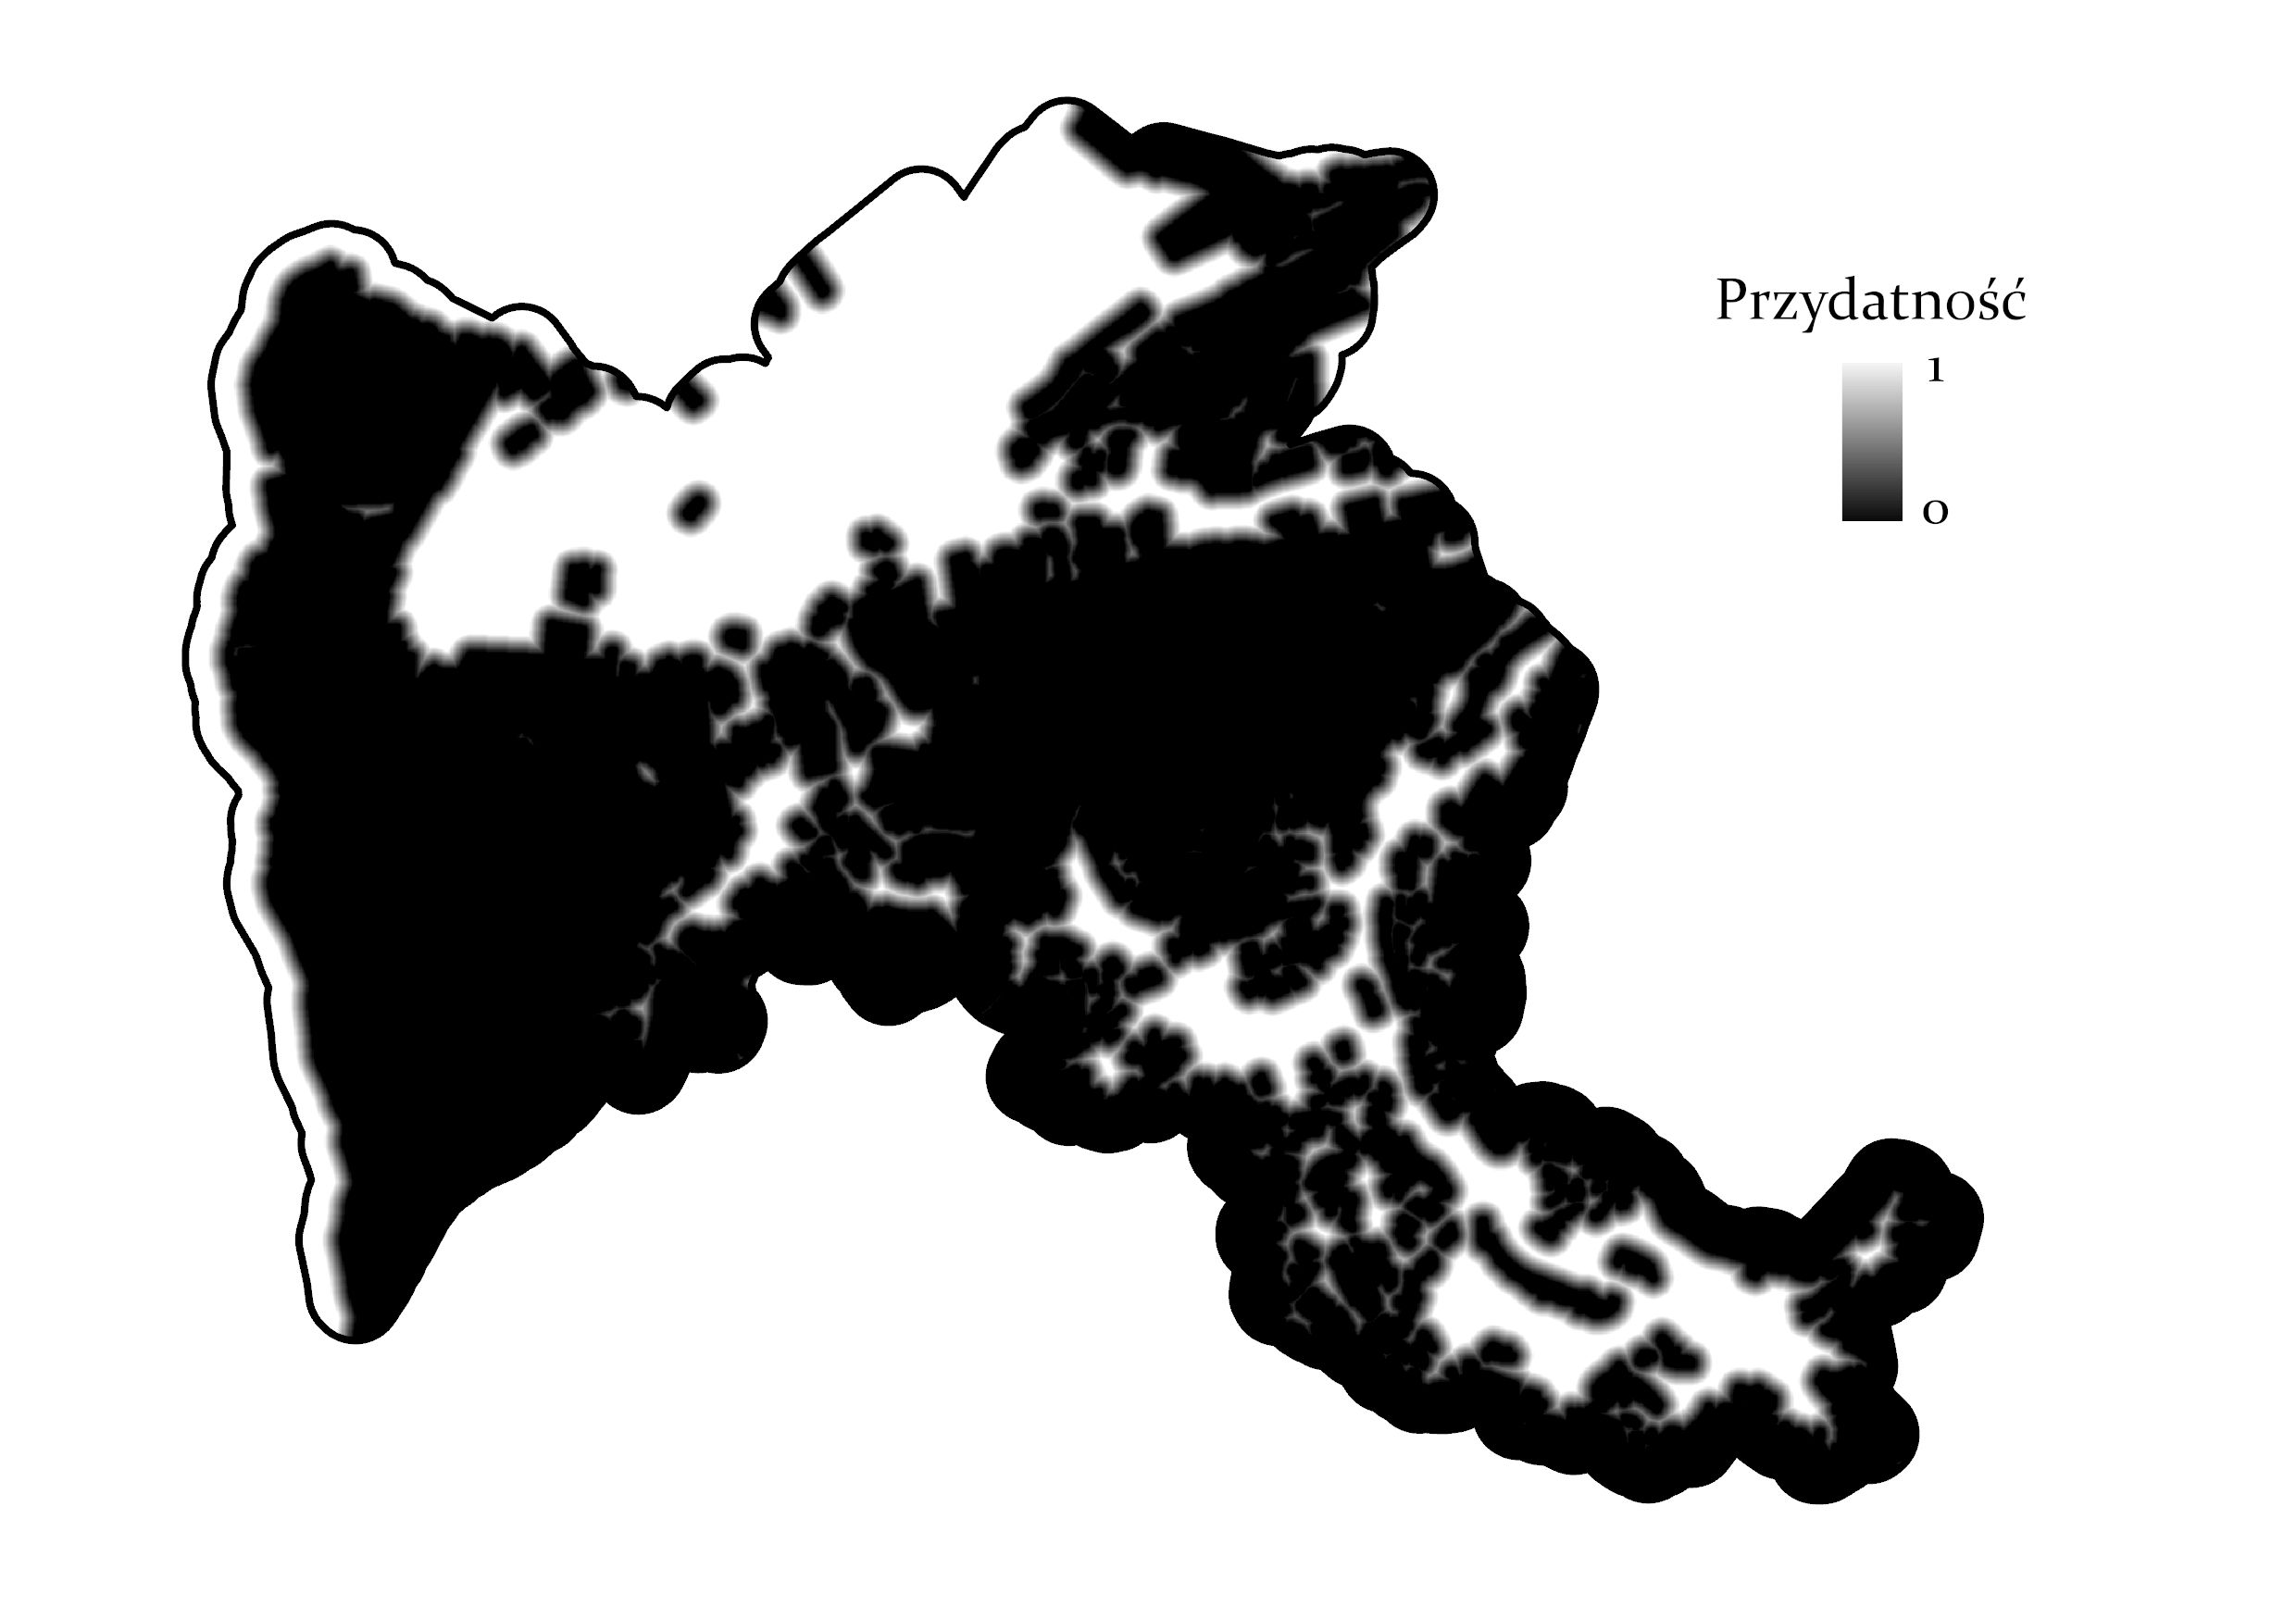
\includegraphics[width=0.75\textwidth]{img/kryterium3-layout.jpg}
    \caption*{Mapa przydatności dla kryterium 3.}
\end{figure}

\begin{figure}[H]
    \centering
    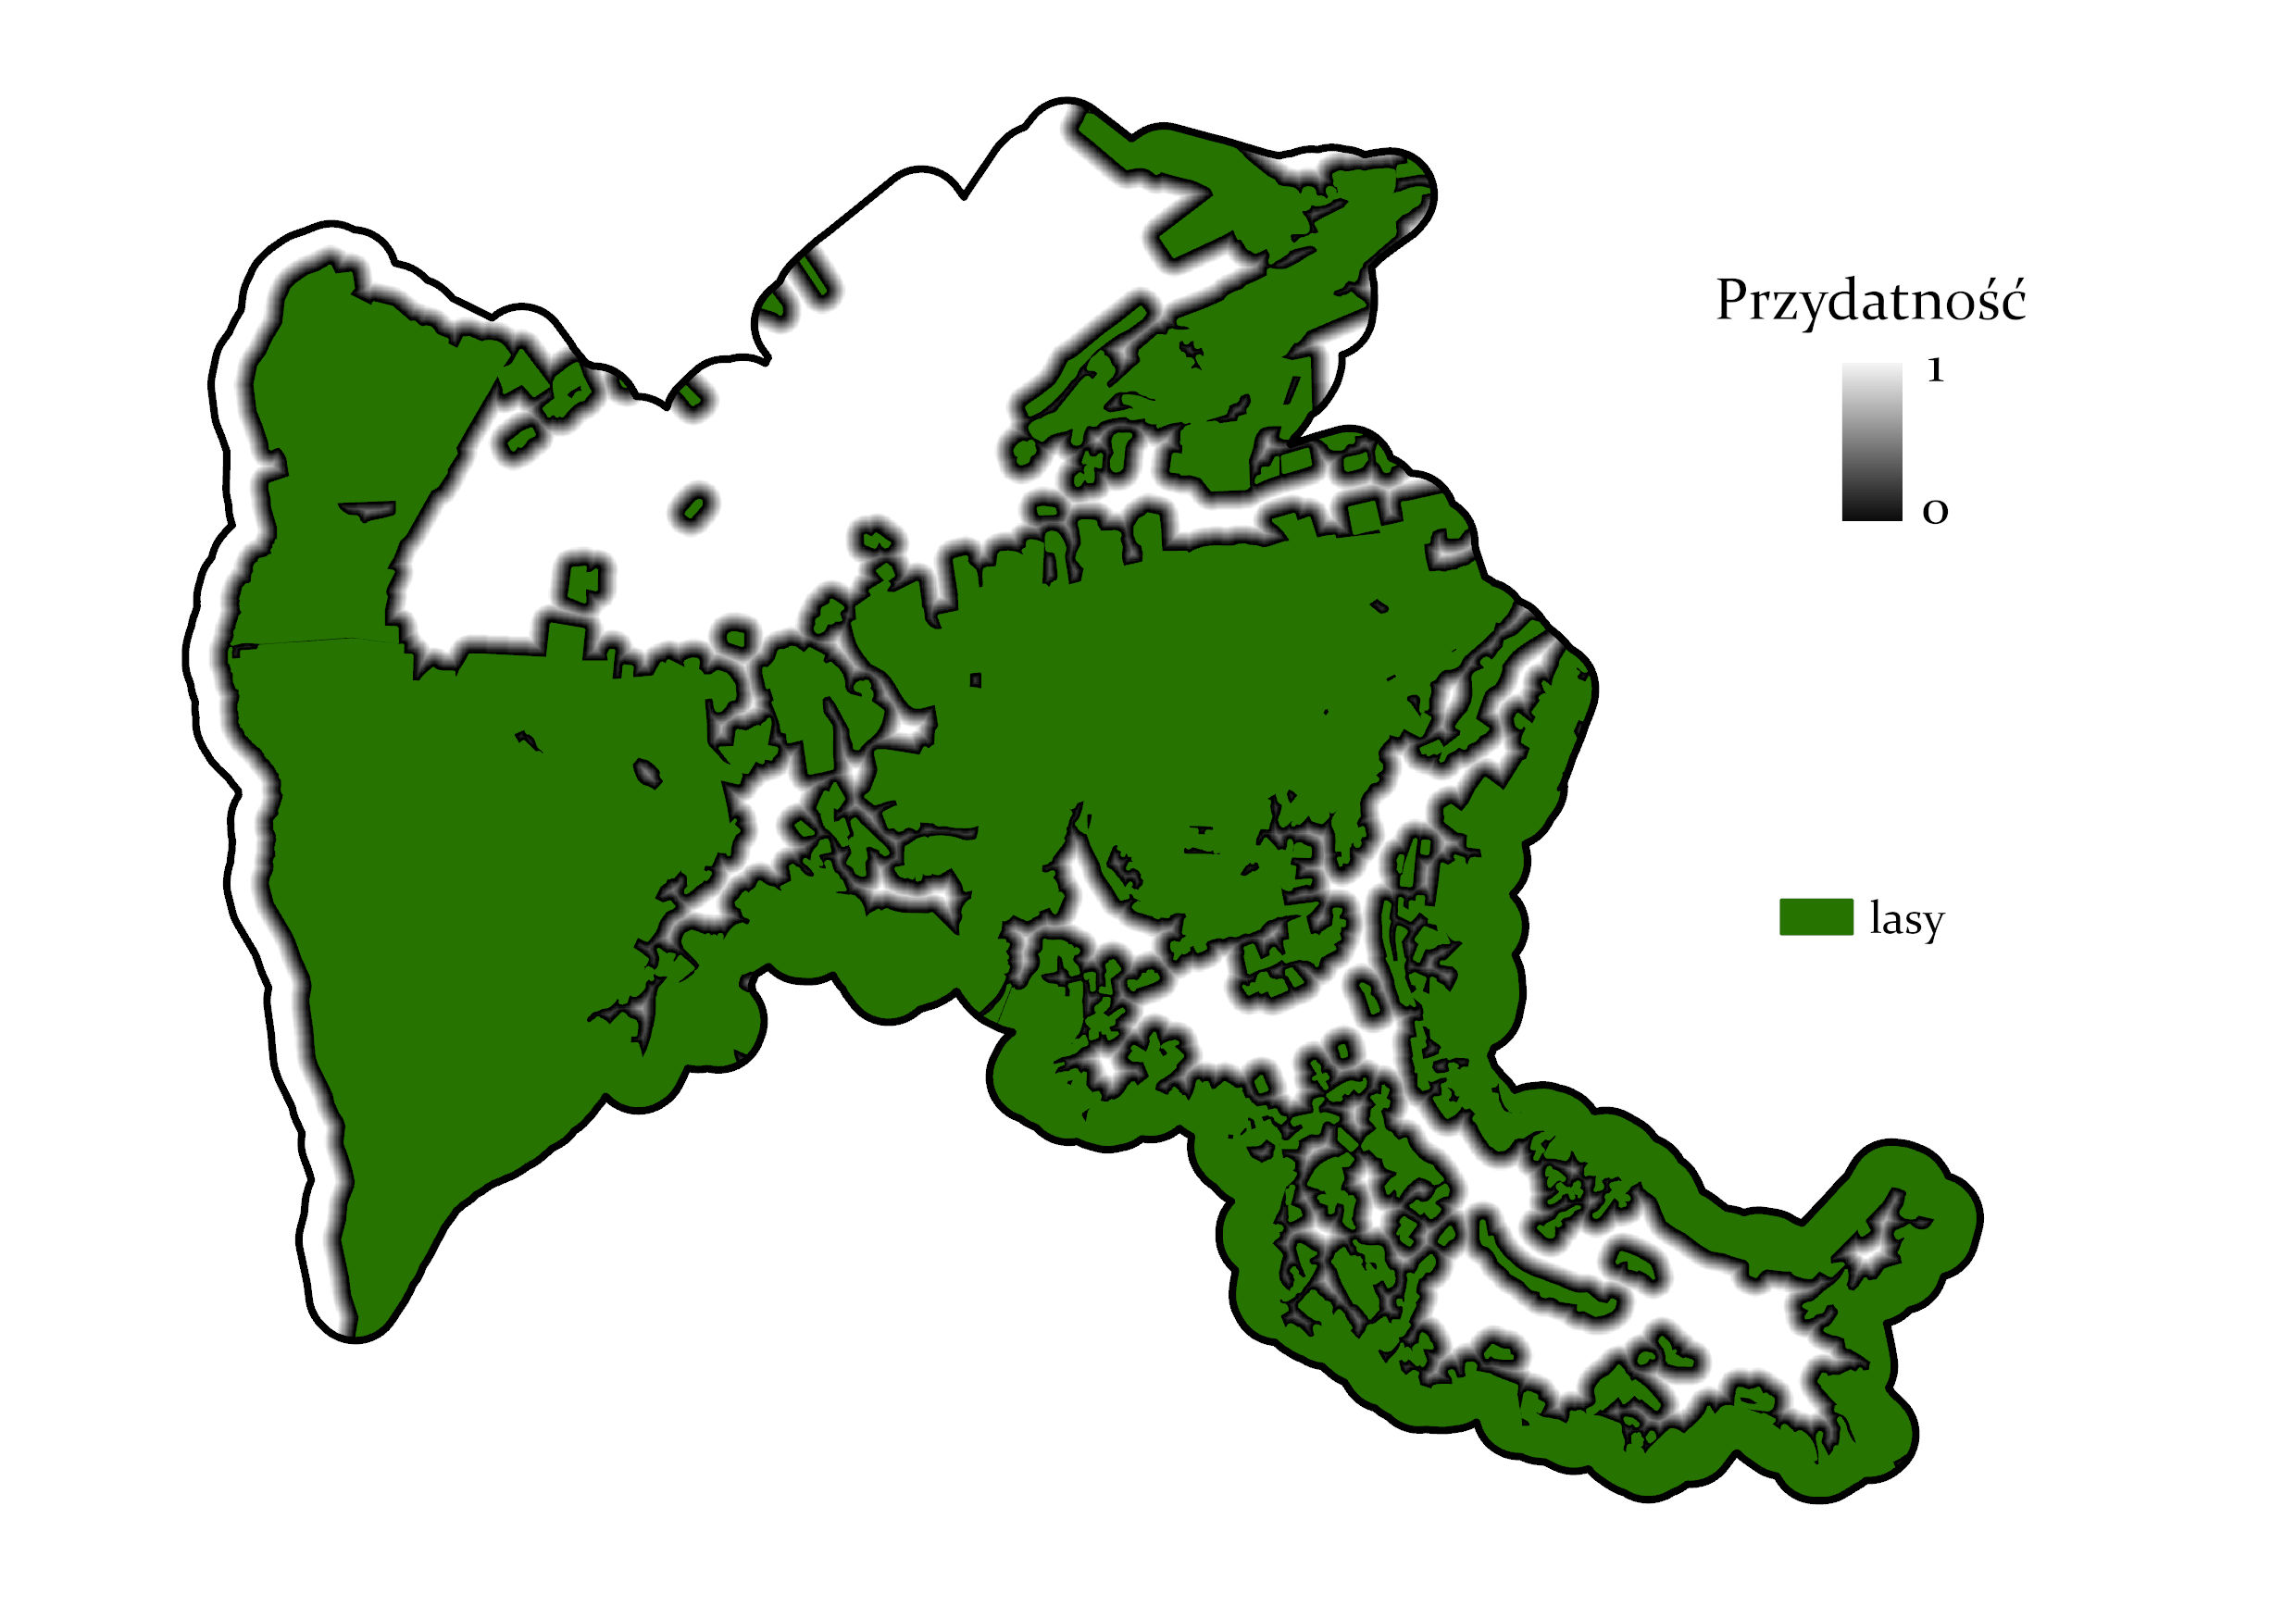
\includegraphics[width=0.75\textwidth]{img/kryterium3-lasy.jpg}
    \caption*{Mapa przydatności dla kryterium 3. zawierająca lasy}
\end{figure}

\newpage
\subsection{Kryterium 4: dostęp do dróg utwardzonych}
\subsubsection{Opis działania}
\begin{figure}[H]
    \centering
    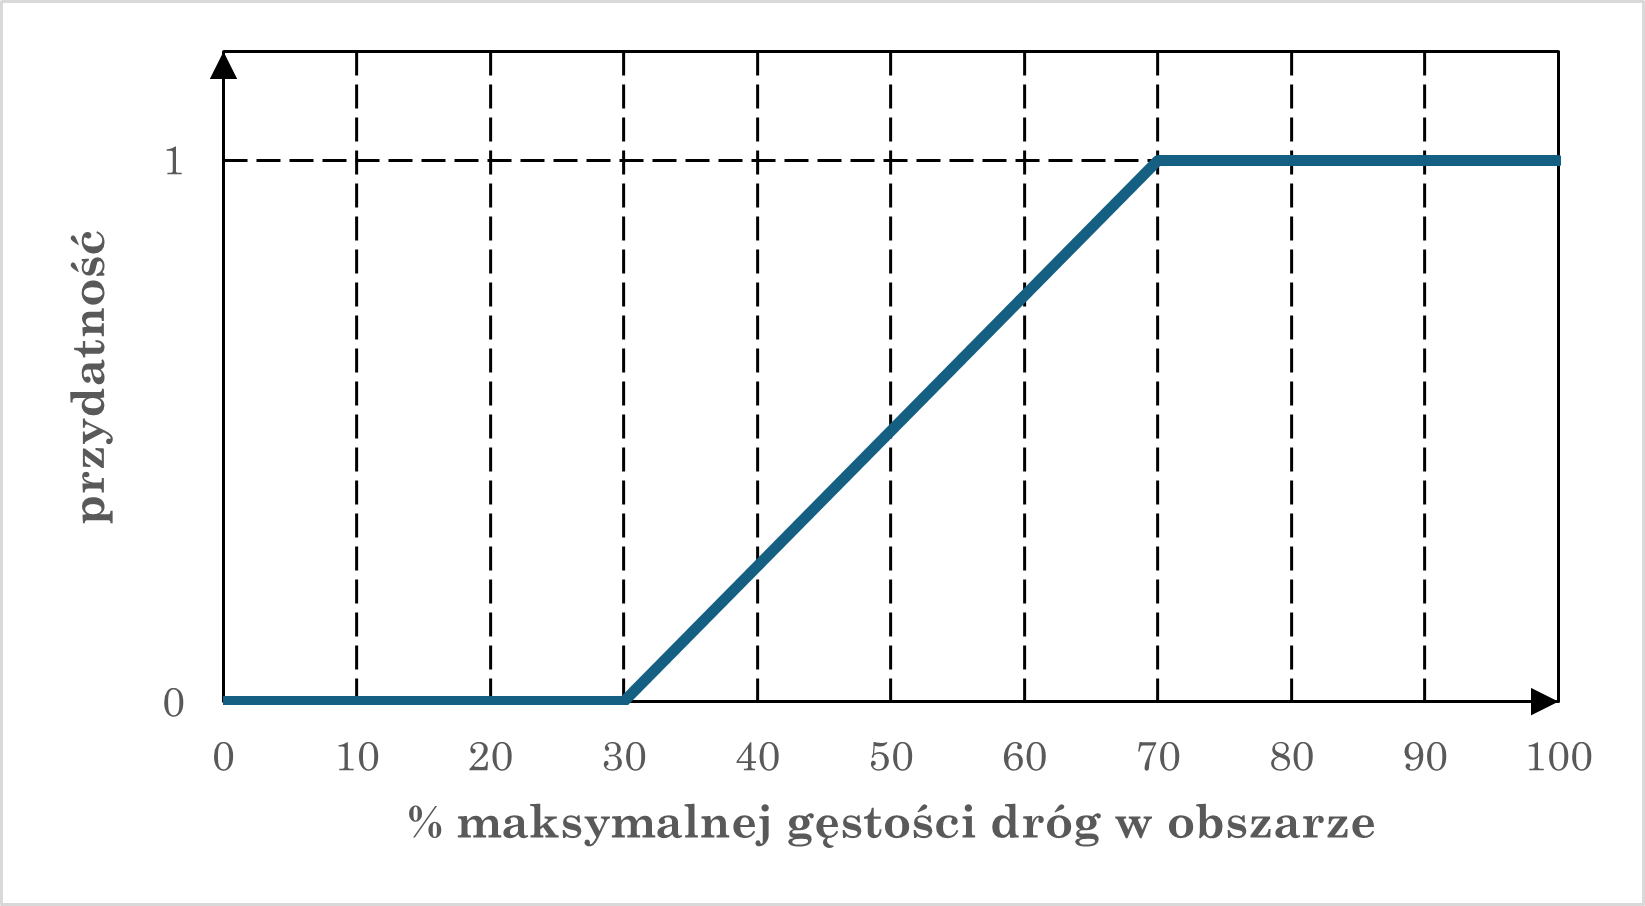
\includegraphics[width=0.75\textwidth]{img/kryterium4-wykres-glowny.png}
    \caption*{Reklasyfikacja dla kryterium 4.}
\end{figure}

\subsubsection{Kod}
\begin{lstlisting}
query = "MATE\_NAWIE IN ('beton', 'bruk', 'kostka kamienna', 'kostka prefabrykowana', 'masa bitumiczna', 'plyty betonowe')"
drogi_utwardzone = arcpy.analysis.Select(drogi, 'drogi_utwardzone', query)

density = arcpy.sa.LineDensity(
    in_polyline_features=drogi_utwardzone,
    population_field=None,
    cell_size=5,
    search_radius=1000,
    area_unit_scale_factor="SQUARE_KILOMETERS",
)
density.save(f'{geobaza}\\drogi_density')

arcpy.management.CalculateStatistics(density)
max_value = density.maximum

kryterium_4 = arcpy.sa.RescaleByFunction(
    in_raster=density,
    transformation_function=f"LINEAR {0.3 * max_value} {0.7 * max_value}",
    from_scale=0,
    to_scale=1   
)
kryterium_4.save(f'{geobaza}\\kryterium_4')
\end{lstlisting}

\subsubsection{Wynik}
\begin{figure}[H]
    \centering
    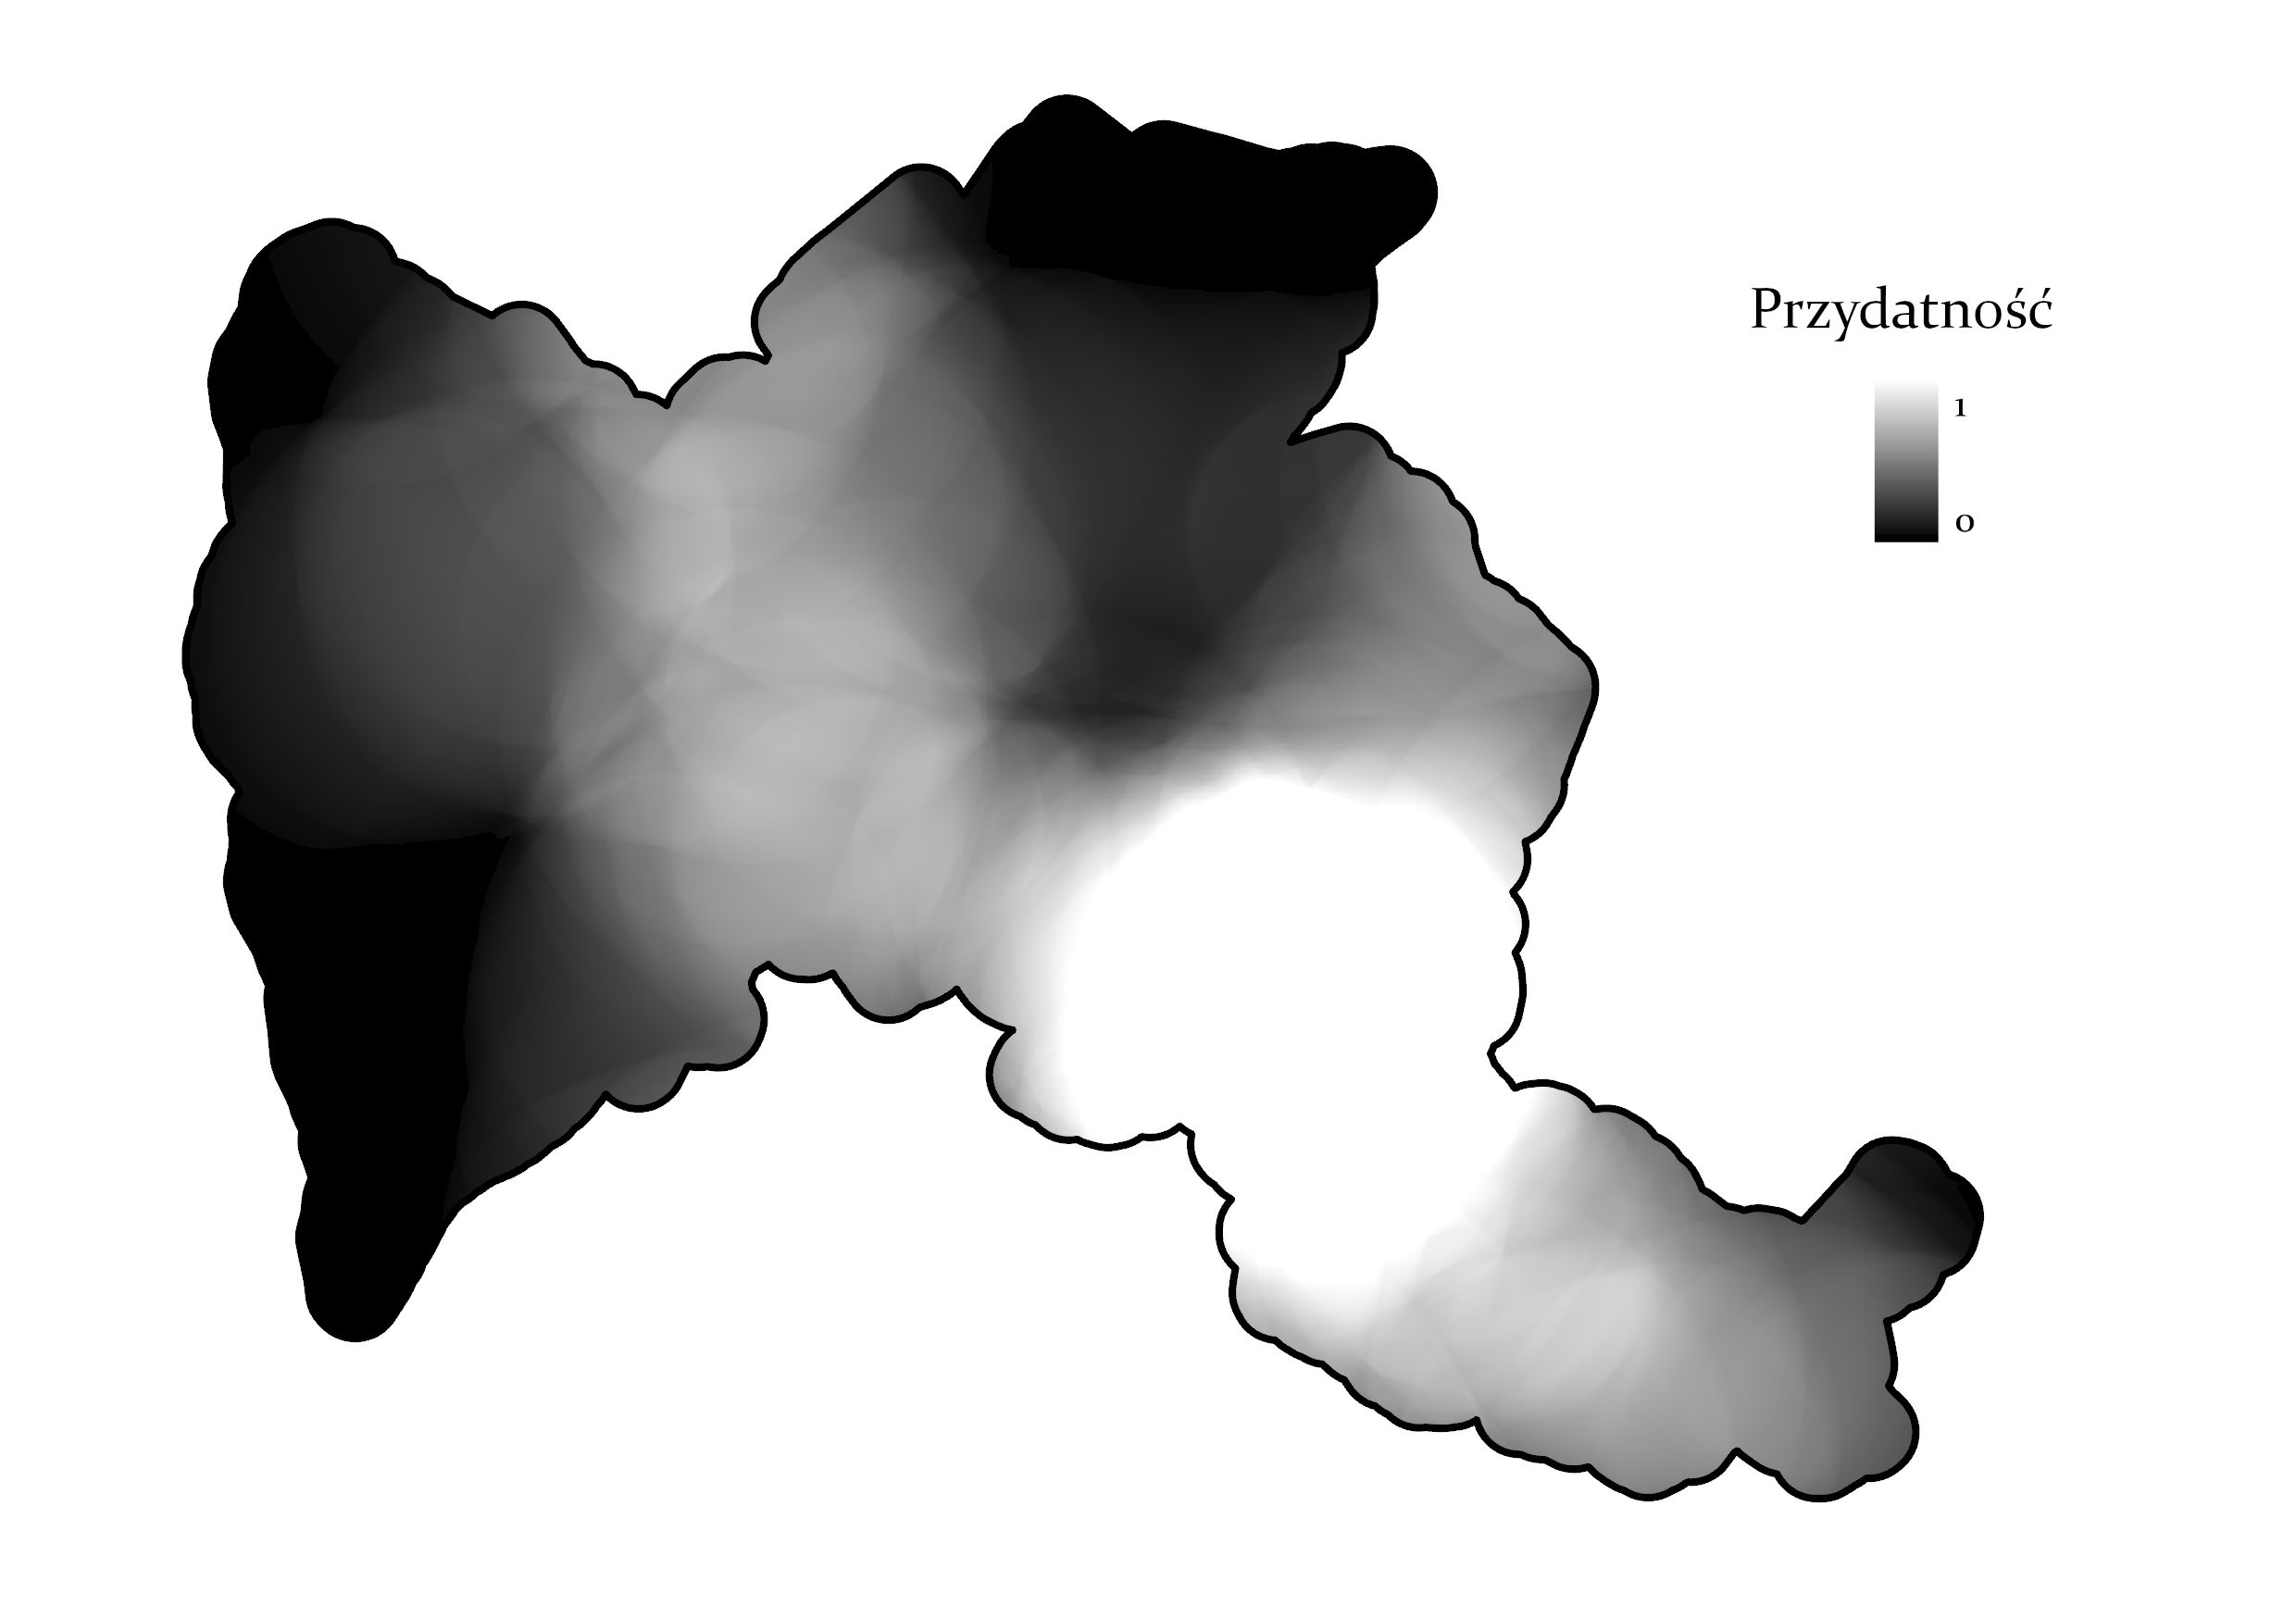
\includegraphics[width=0.75\textwidth]{img/kryterium4-layout.jpg}
    \caption*{Mapa przydatności dla kryterium 4.}
\end{figure}

\begin{figure}[H]
    \centering
    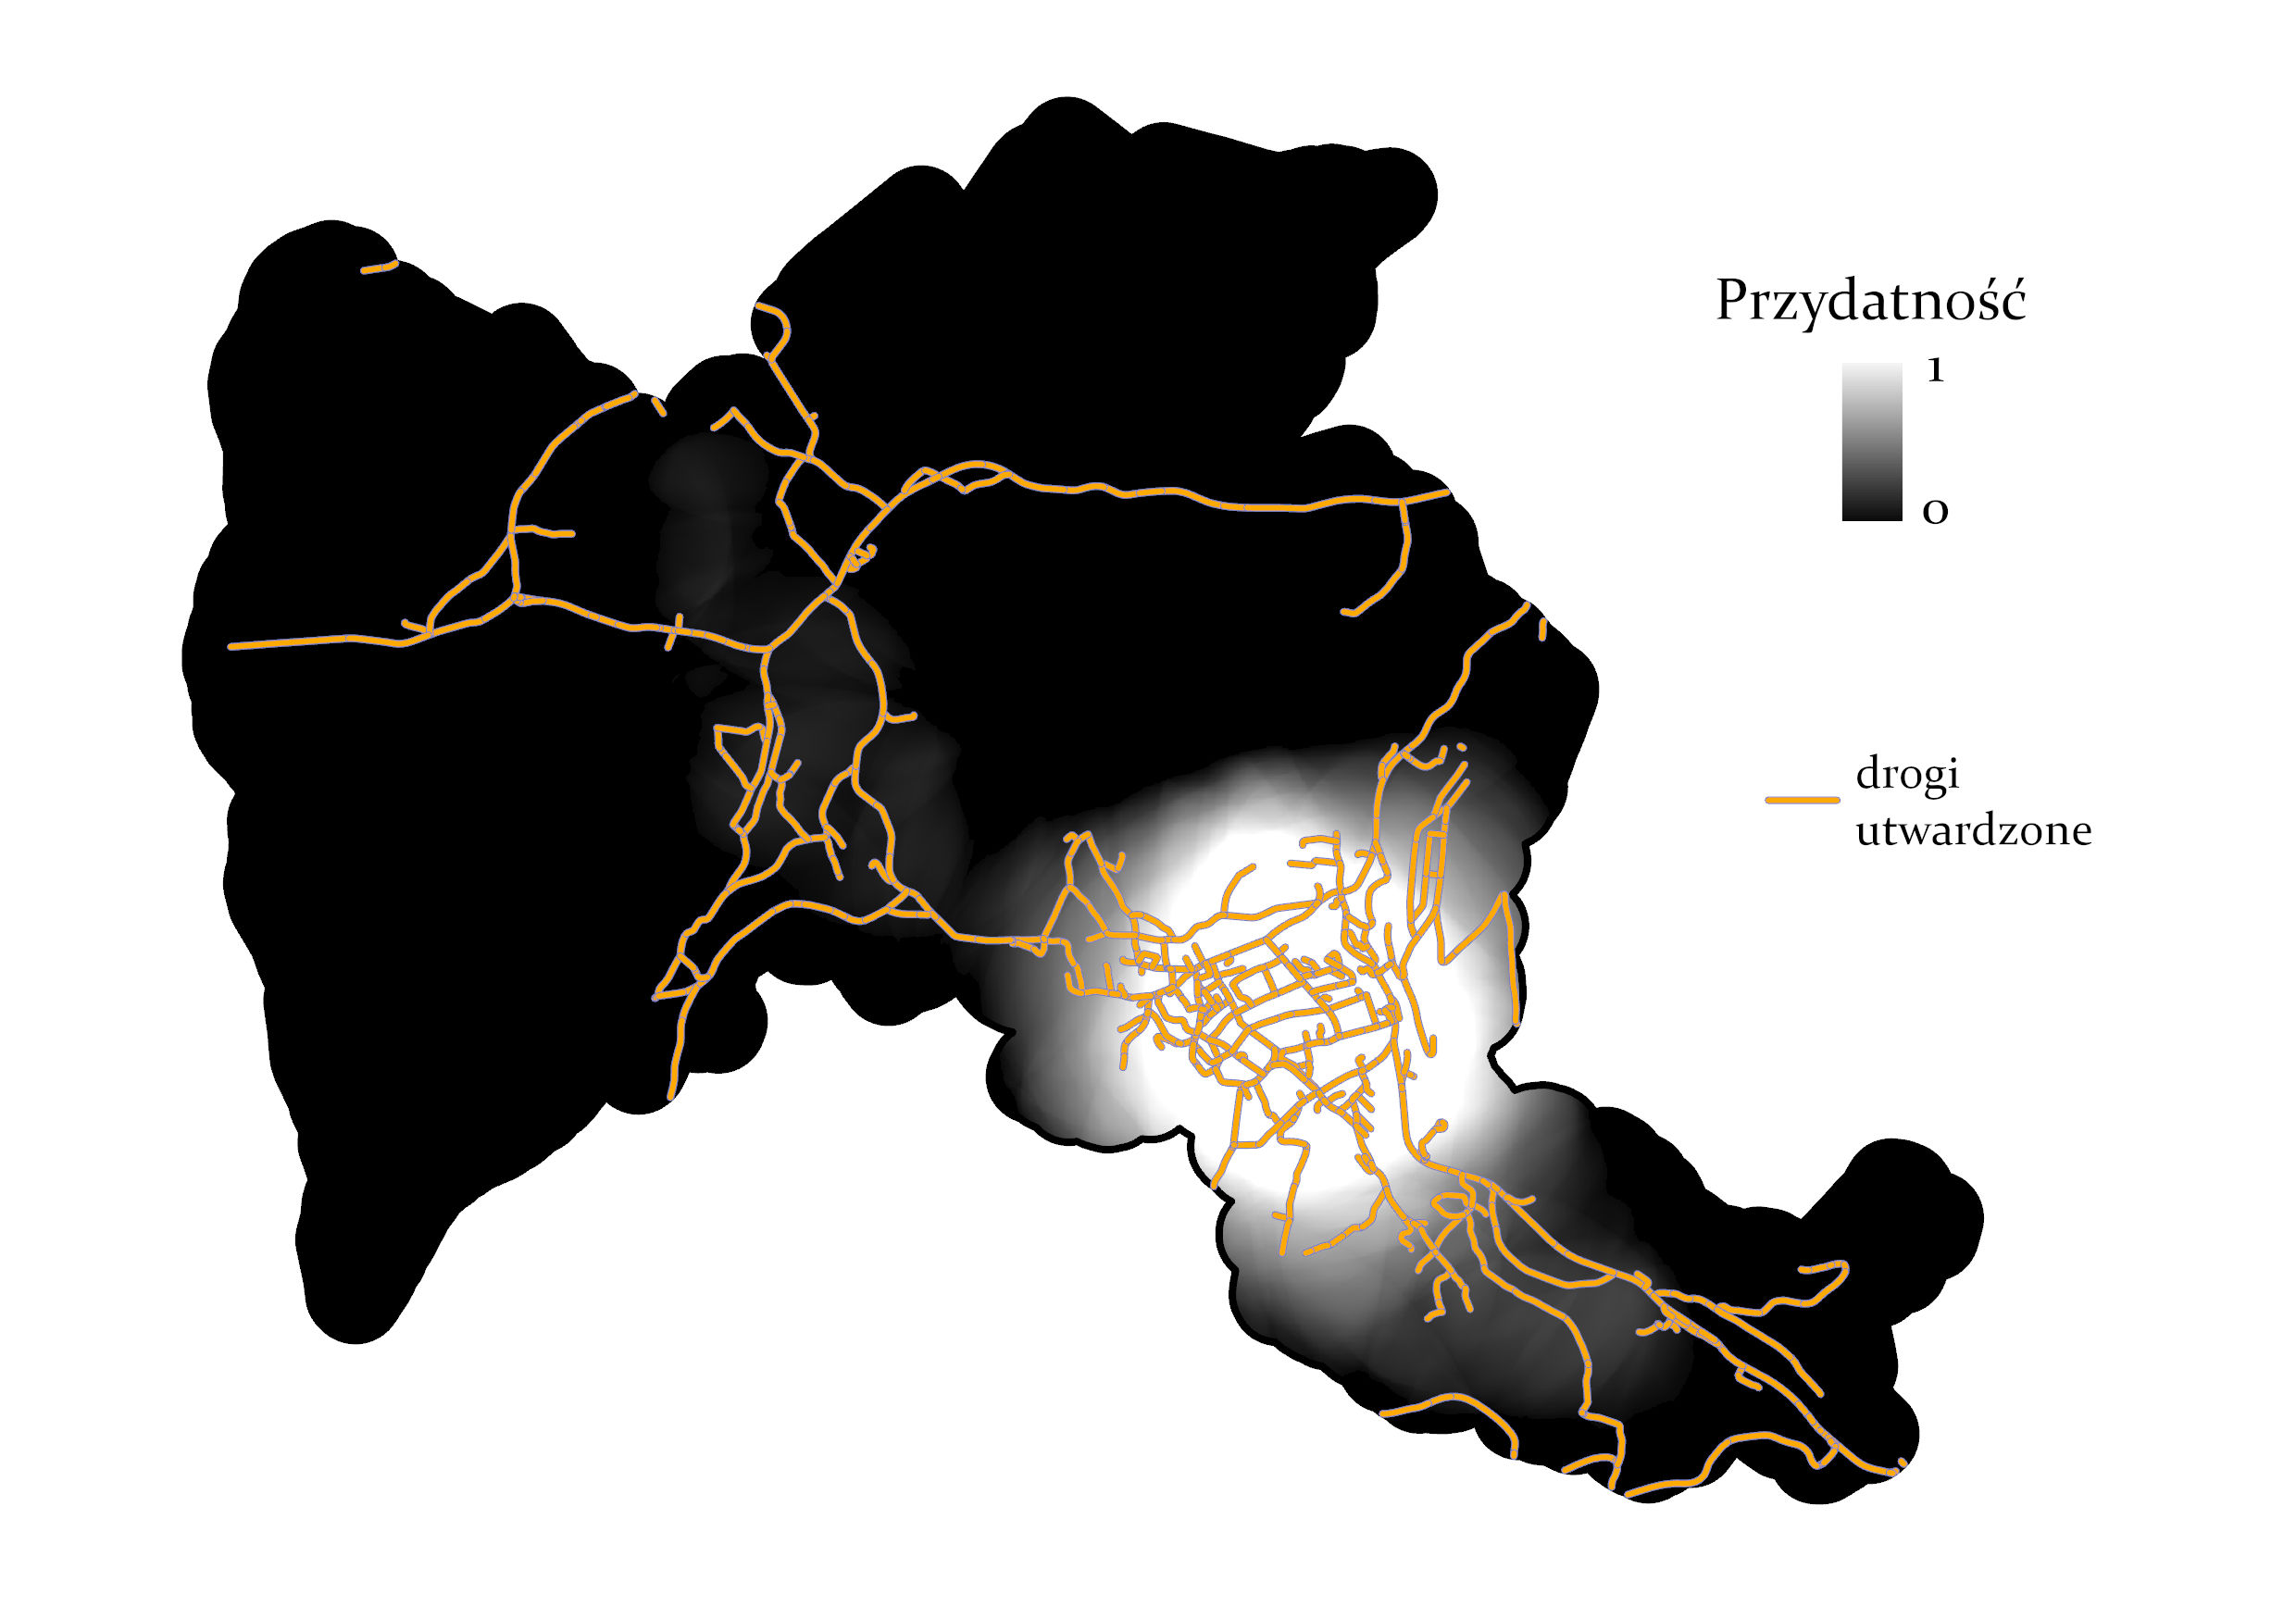
\includegraphics[width=0.75\textwidth]{img/kryterium4-drogi.jpg}
    \caption*{Mapa przydatności dla kryterium 4. zawierająca drogi utwardzone}
\end{figure}

\newpage
\subsection{Kryterium 5: nachylenie stoków}
\subsubsection{Opis działania}
\begin{figure}[H]
    \centering
    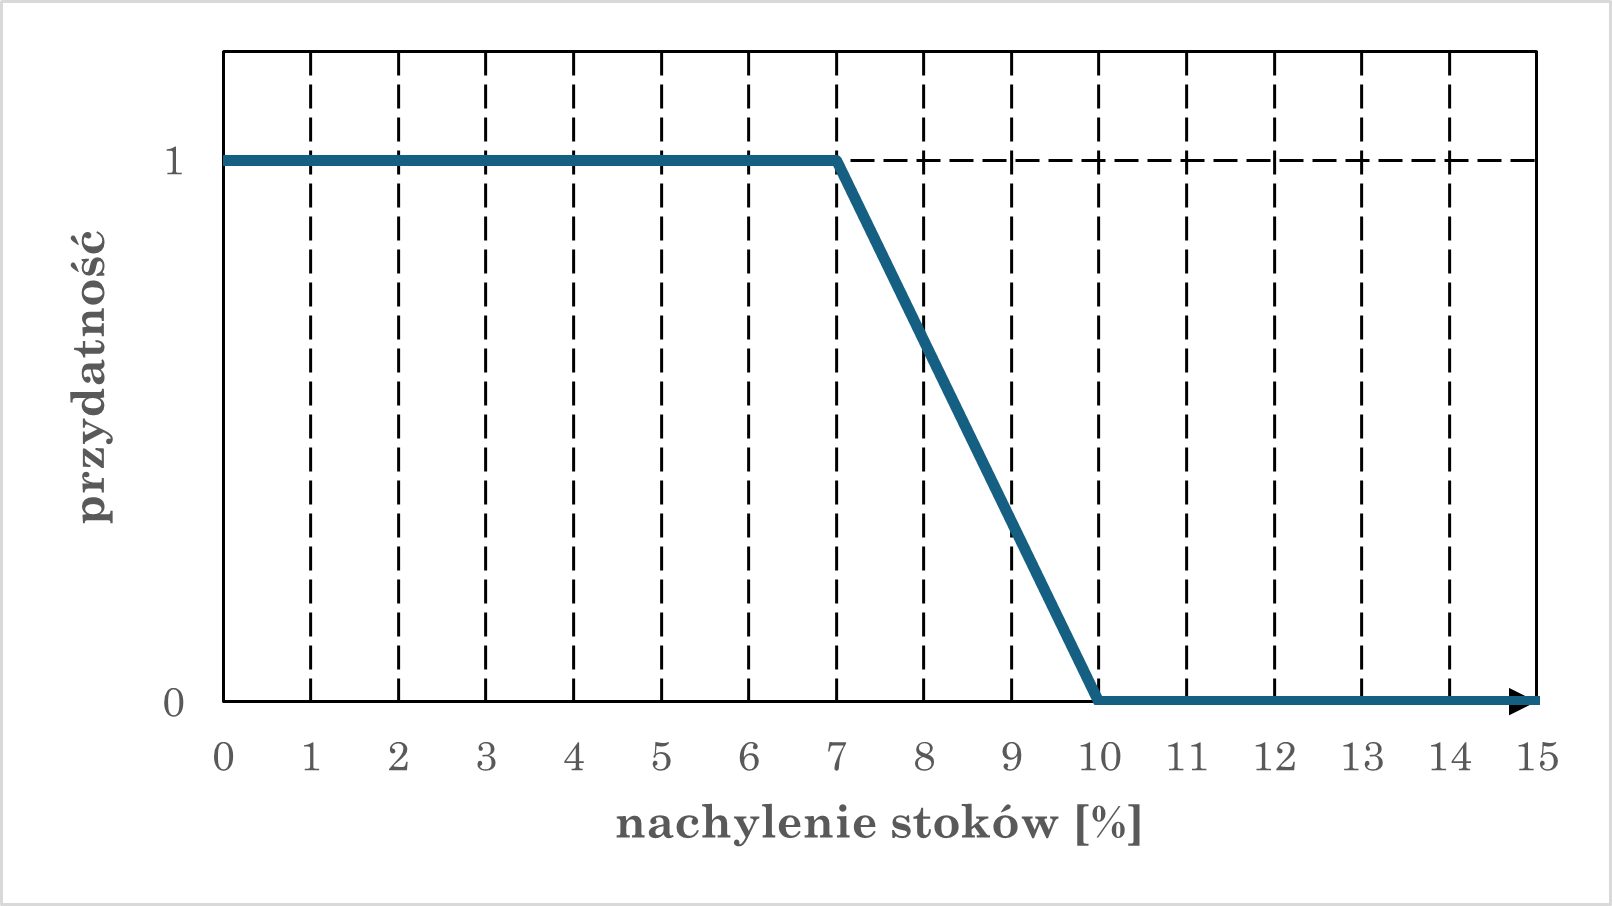
\includegraphics[width=0.75\textwidth]{img/kryterium5-wykres-glowny.png}
    \caption*{Reklasyfikacja dla kryterium 5.}
\end{figure}

\subsubsection{Kod}
\begin{lstlisting}
arcpy.ddd.Slope(nmt, "slope", "PERCENT_RISE", 1)
slope_fuzzy = arcpy.sa.FuzzyMembership("slope", fuzzy_function="LINEAR 10 7")
slope_fuzzy.save(f'{geobaza}\\kryterium_5')
\end{lstlisting}

\subsubsection{Wynik}
\begin{figure}[H]
    \centering
    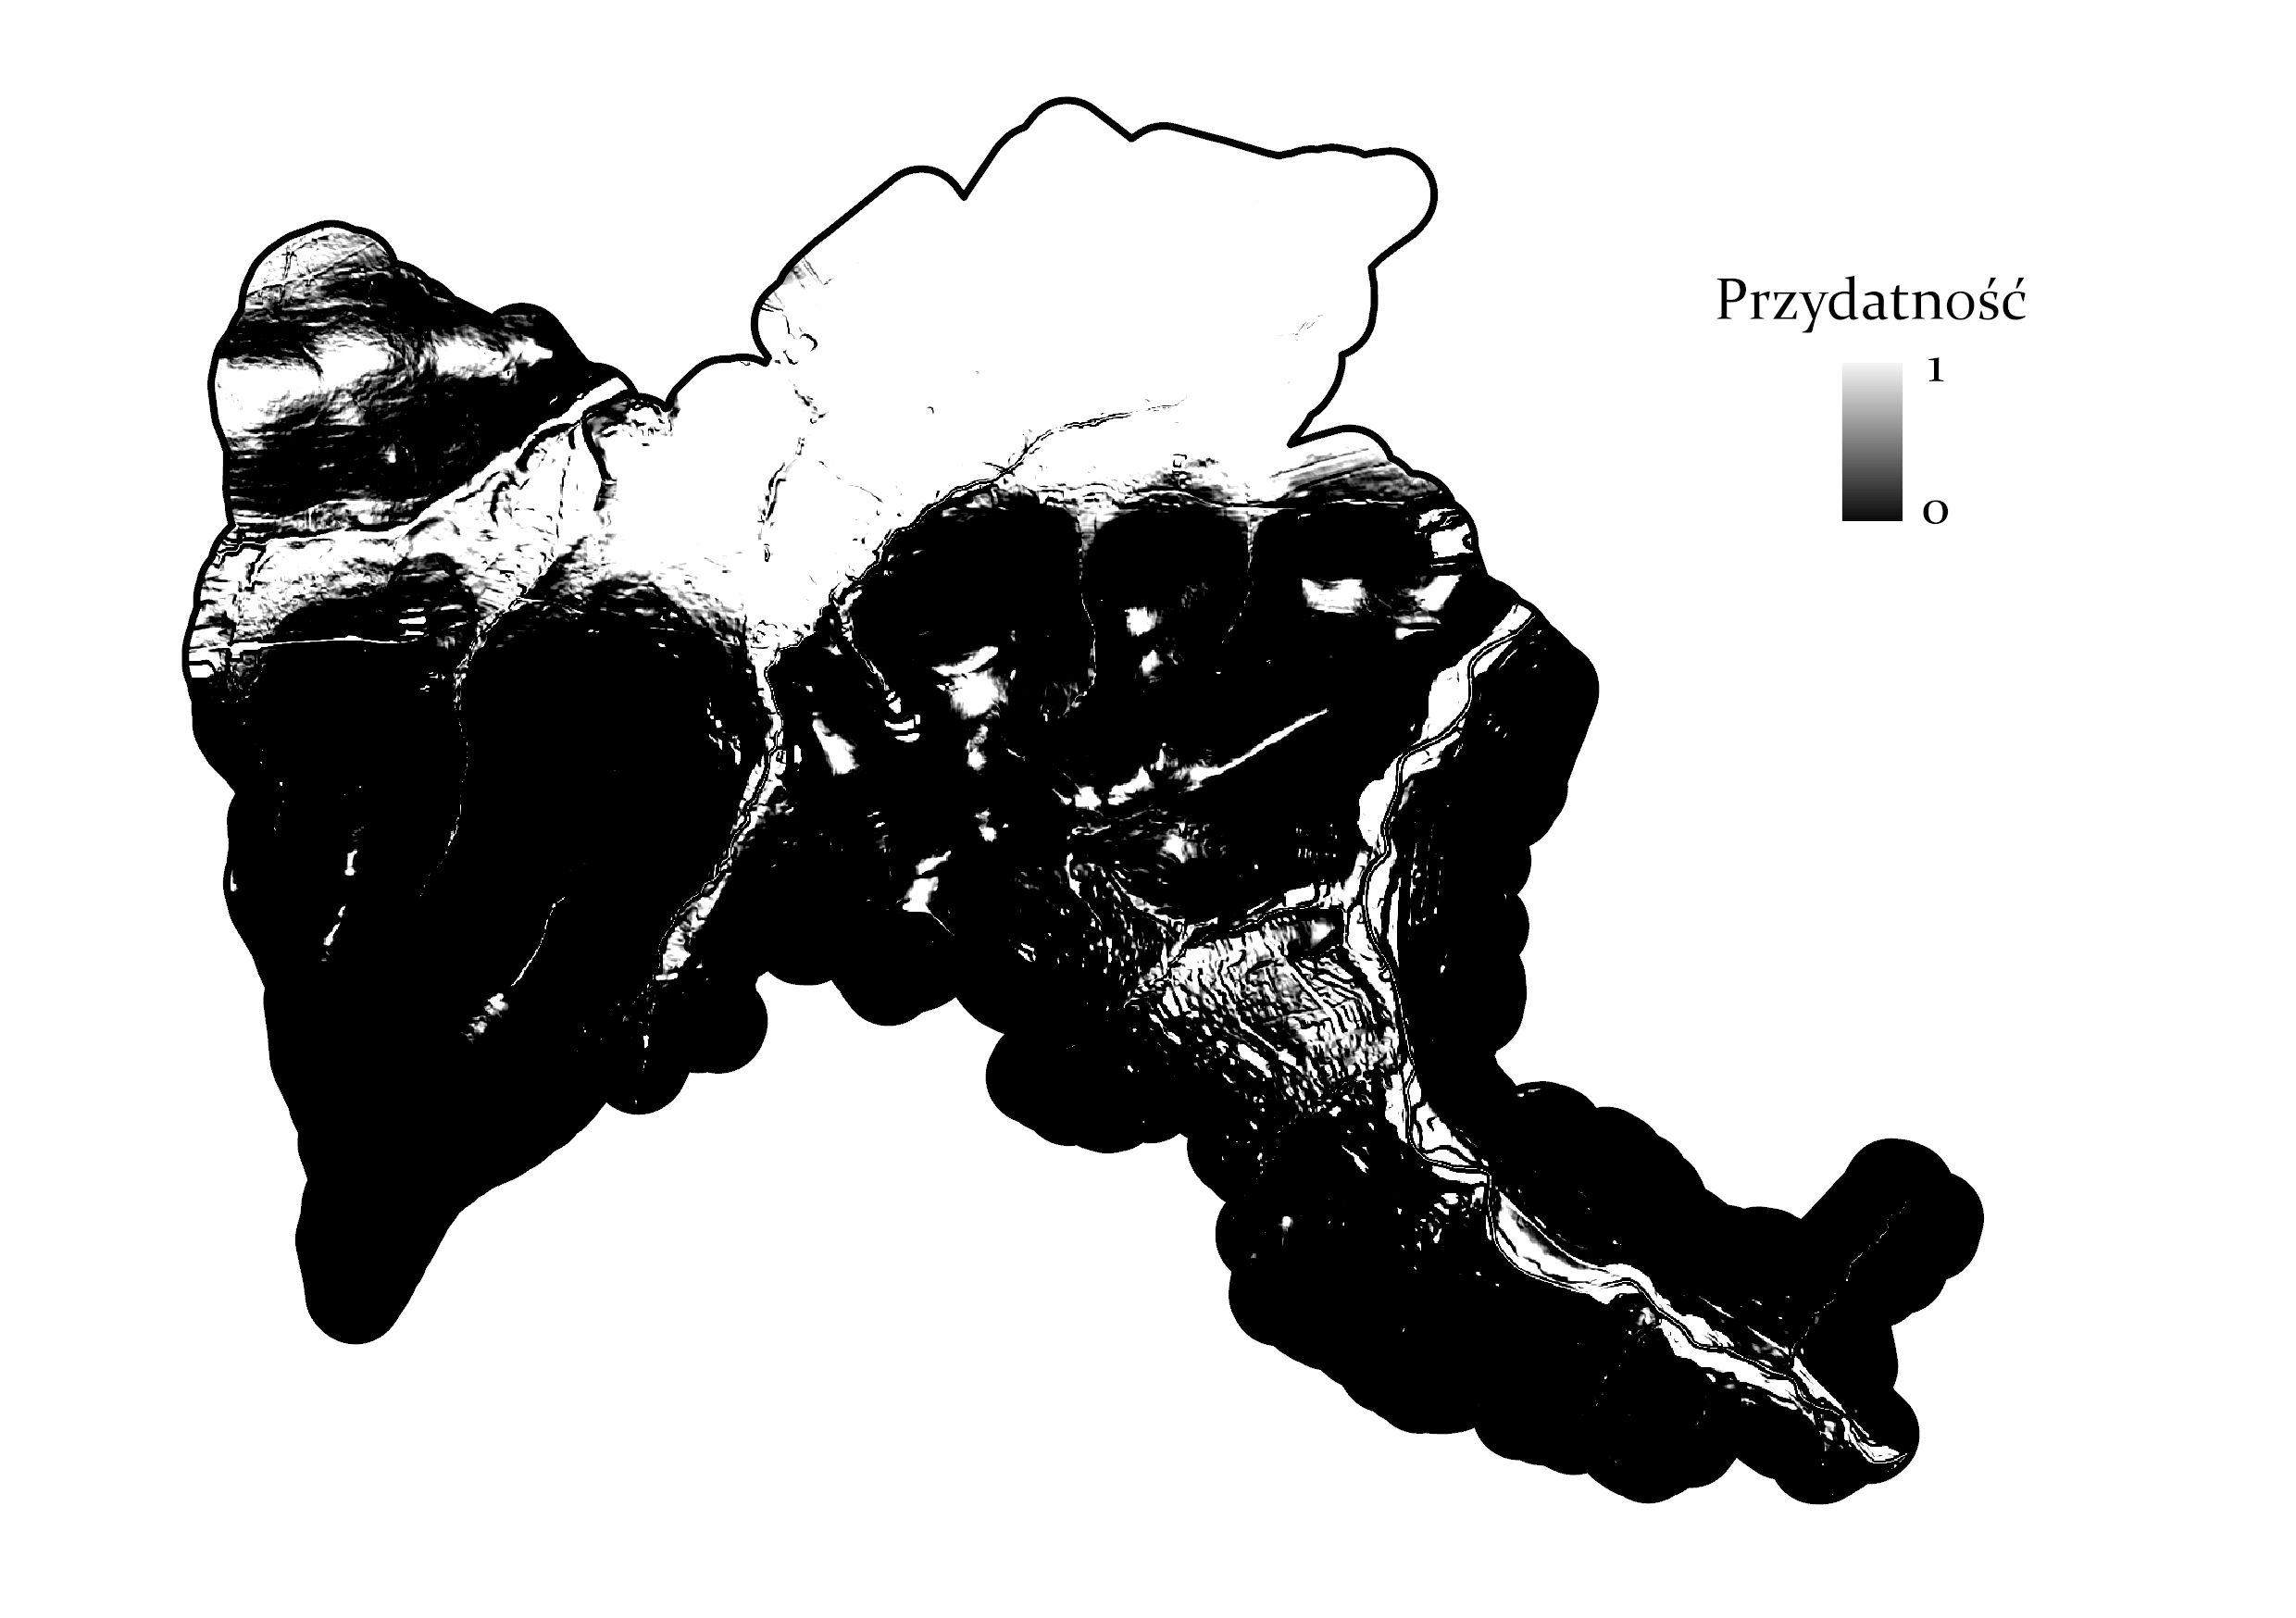
\includegraphics[width=0.75\textwidth]{img/kryterium5-layout.jpg}
    \caption*{Mapa przydatności dla kryterium 5.}
\end{figure}

\begin{figure}[H]
    \centering
    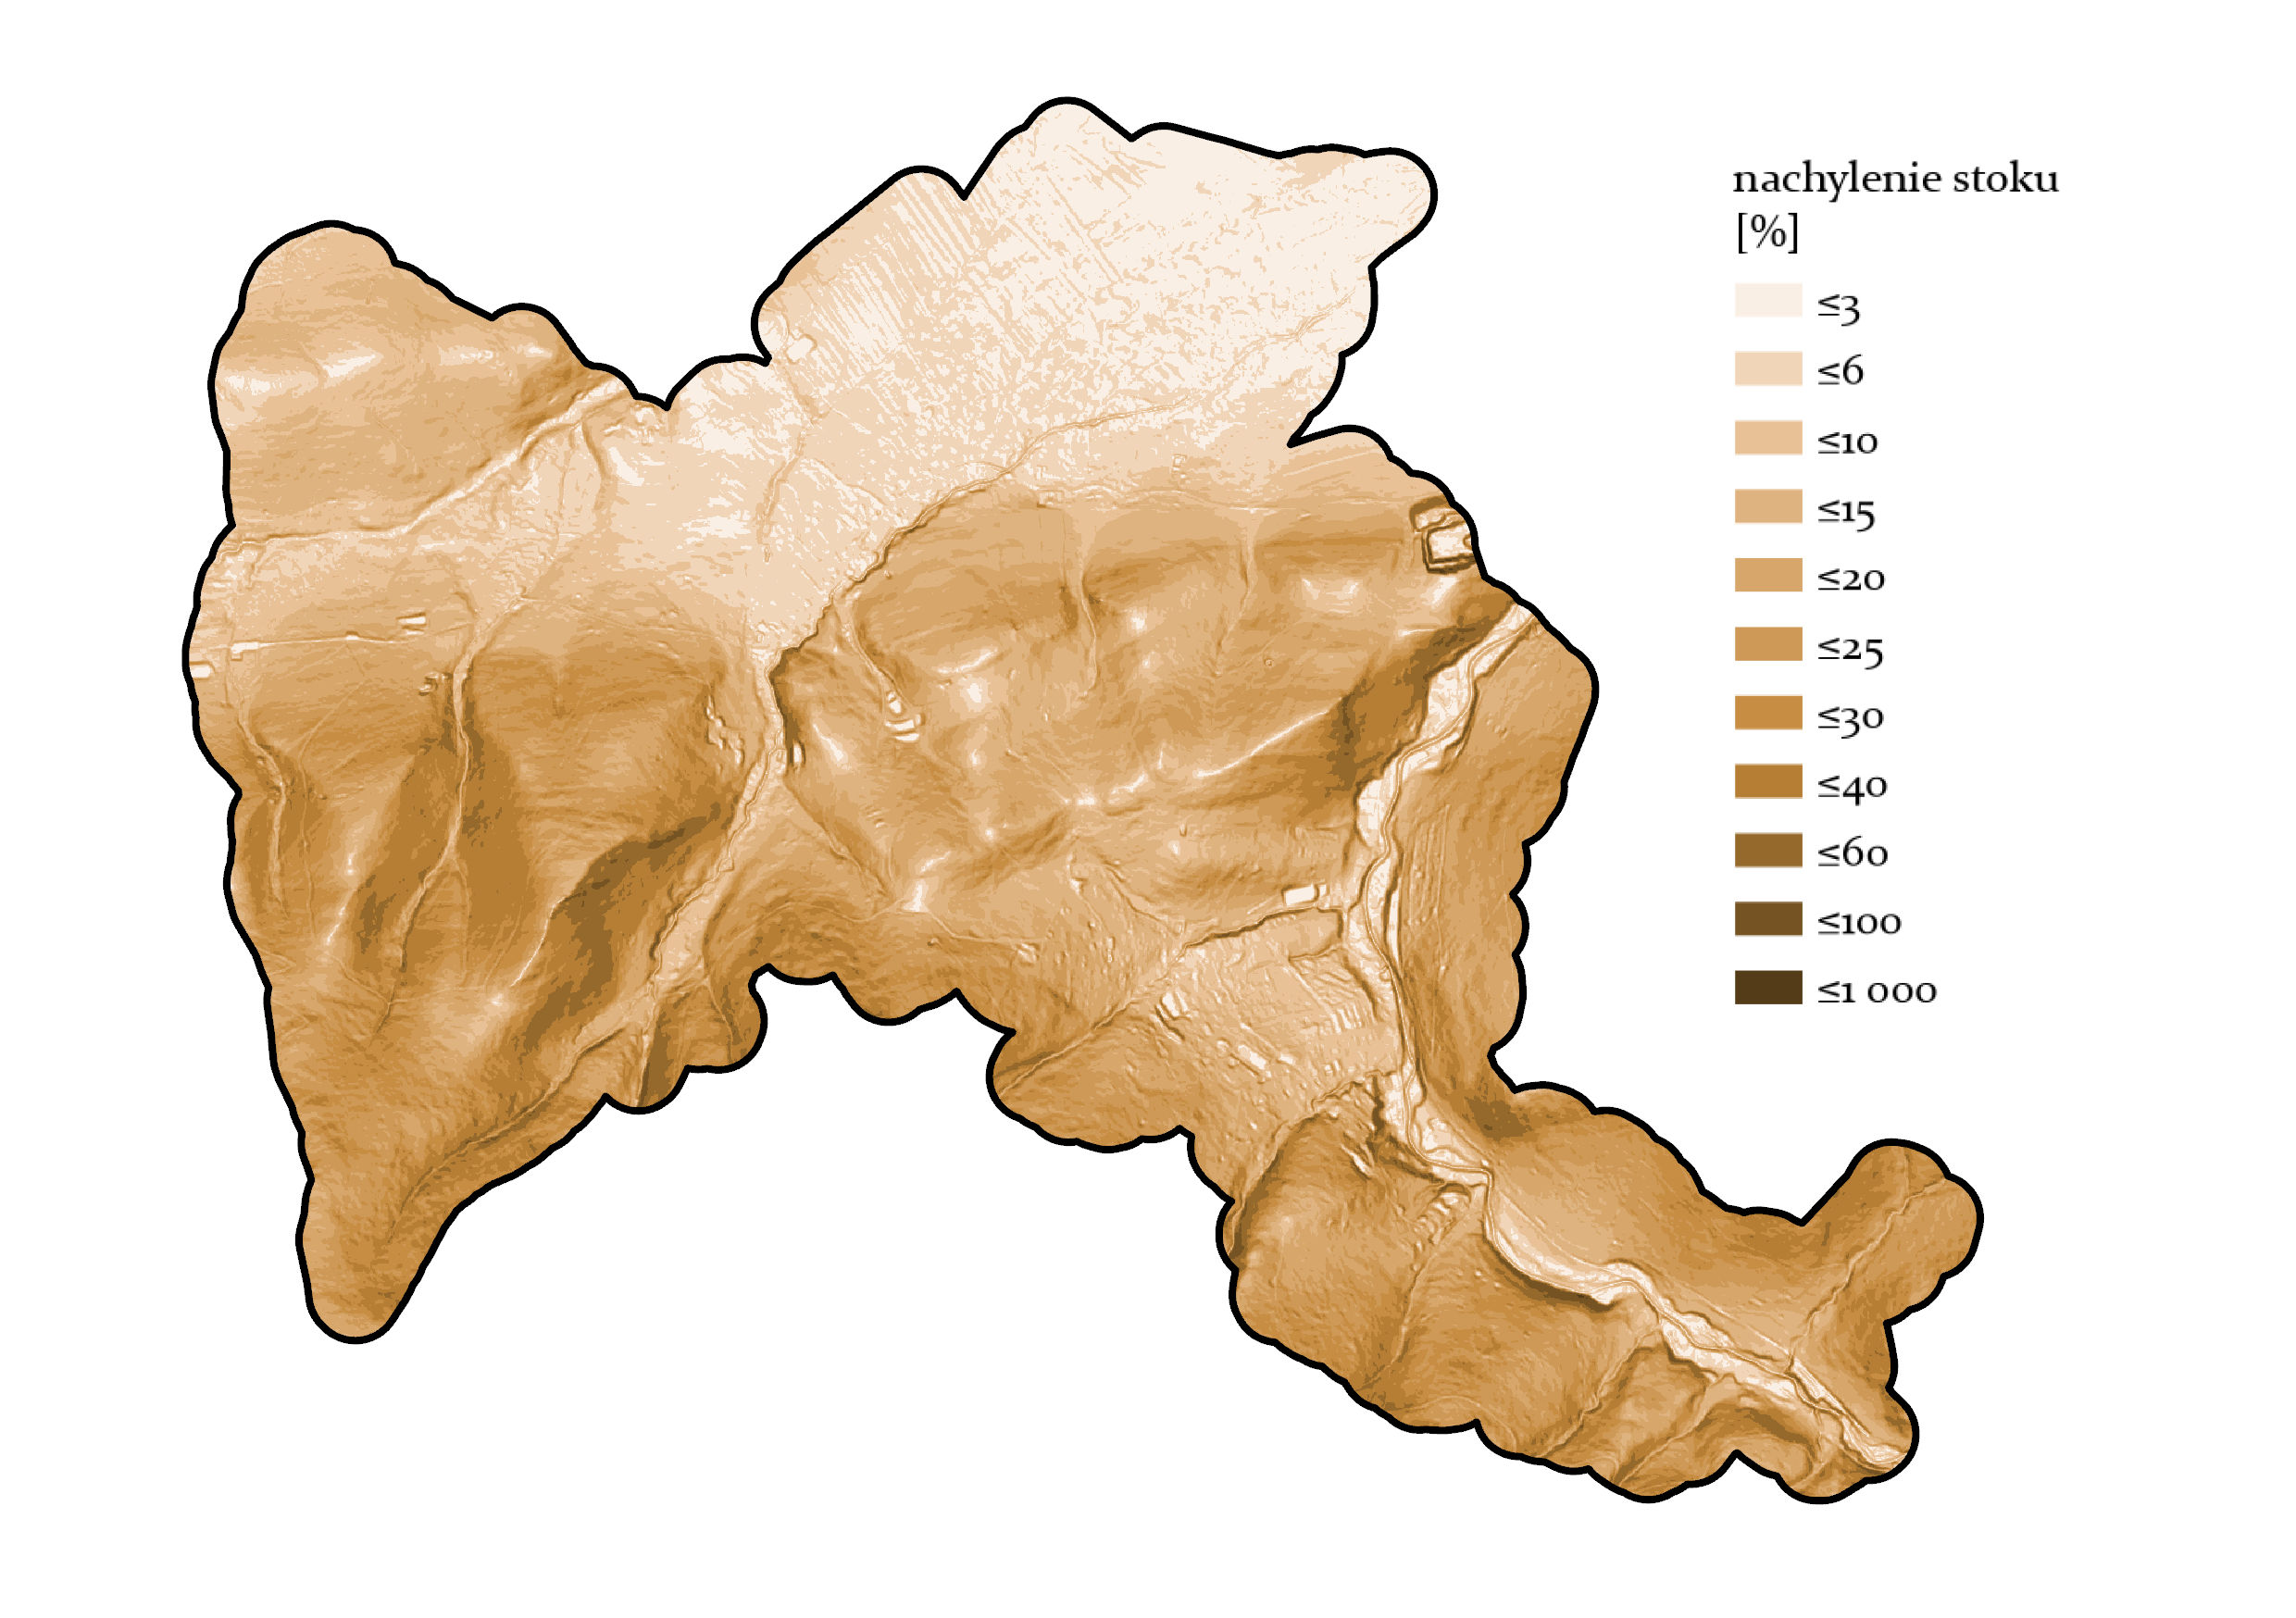
\includegraphics[width=0.75\textwidth]{img/kryterium5-stoki.jpg}
    \caption*{Mapa nachyleń stoków wykorzystana podczas sprawdzania kryterium 5.}
\end{figure}

\newpage
\subsection{Kryterium 6: dostęp do światła słonecznego}
\subsubsection{Opis działania}
\begin{figure}[H]
    \centering
    \begin{minipage}{0.48\textwidth}
        \centering
        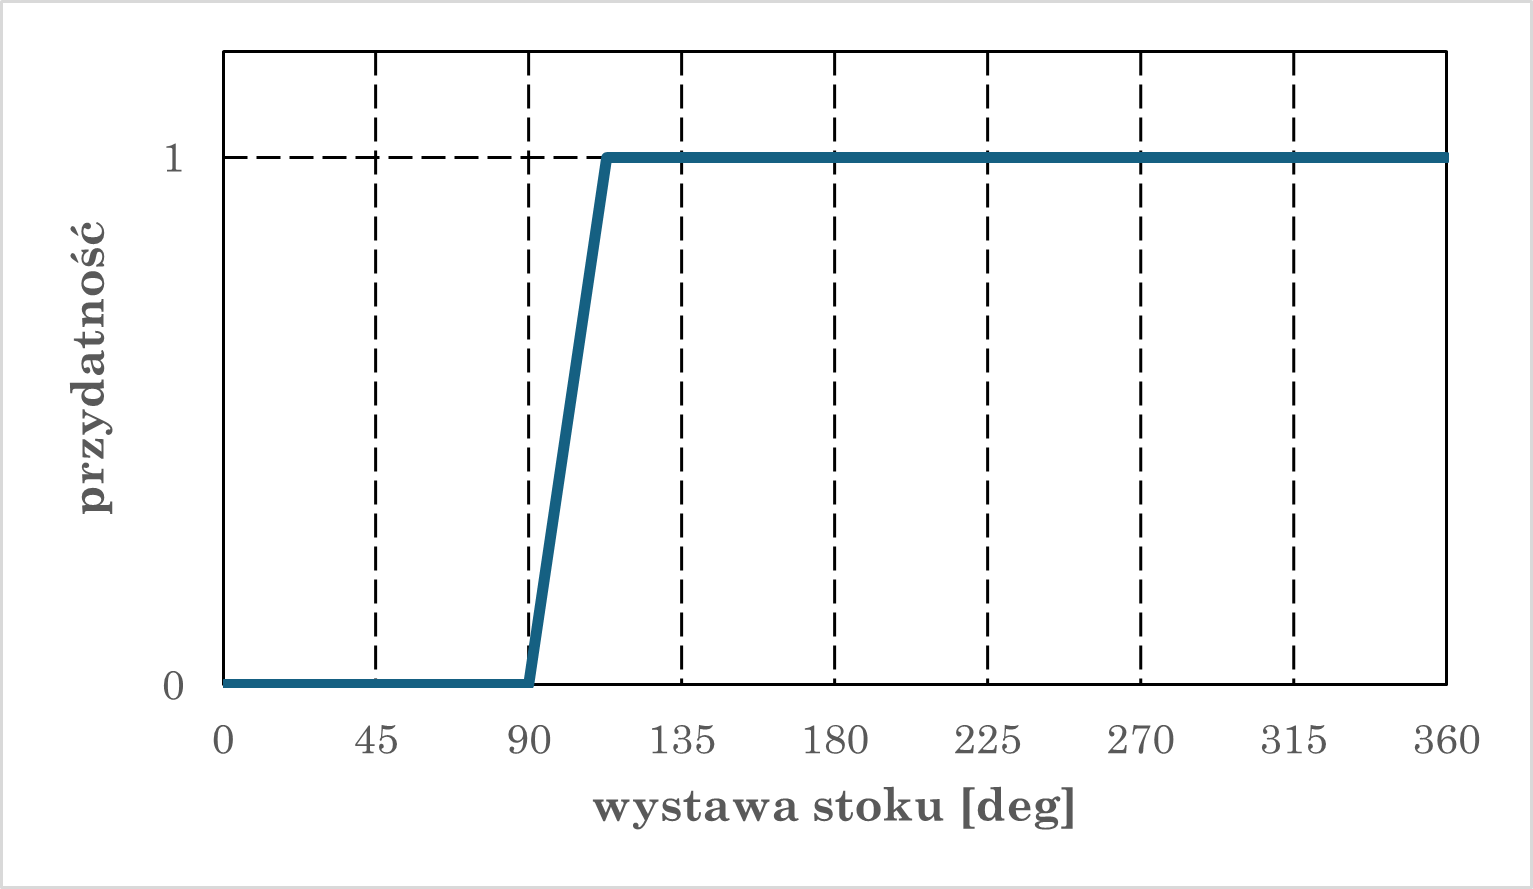
\includegraphics[width=\linewidth]{img/kryterium6-wykres-pierwszy.png}
        \caption*{}
    \end{minipage}
    \begin{minipage}{0.48\textwidth}
        \centering
        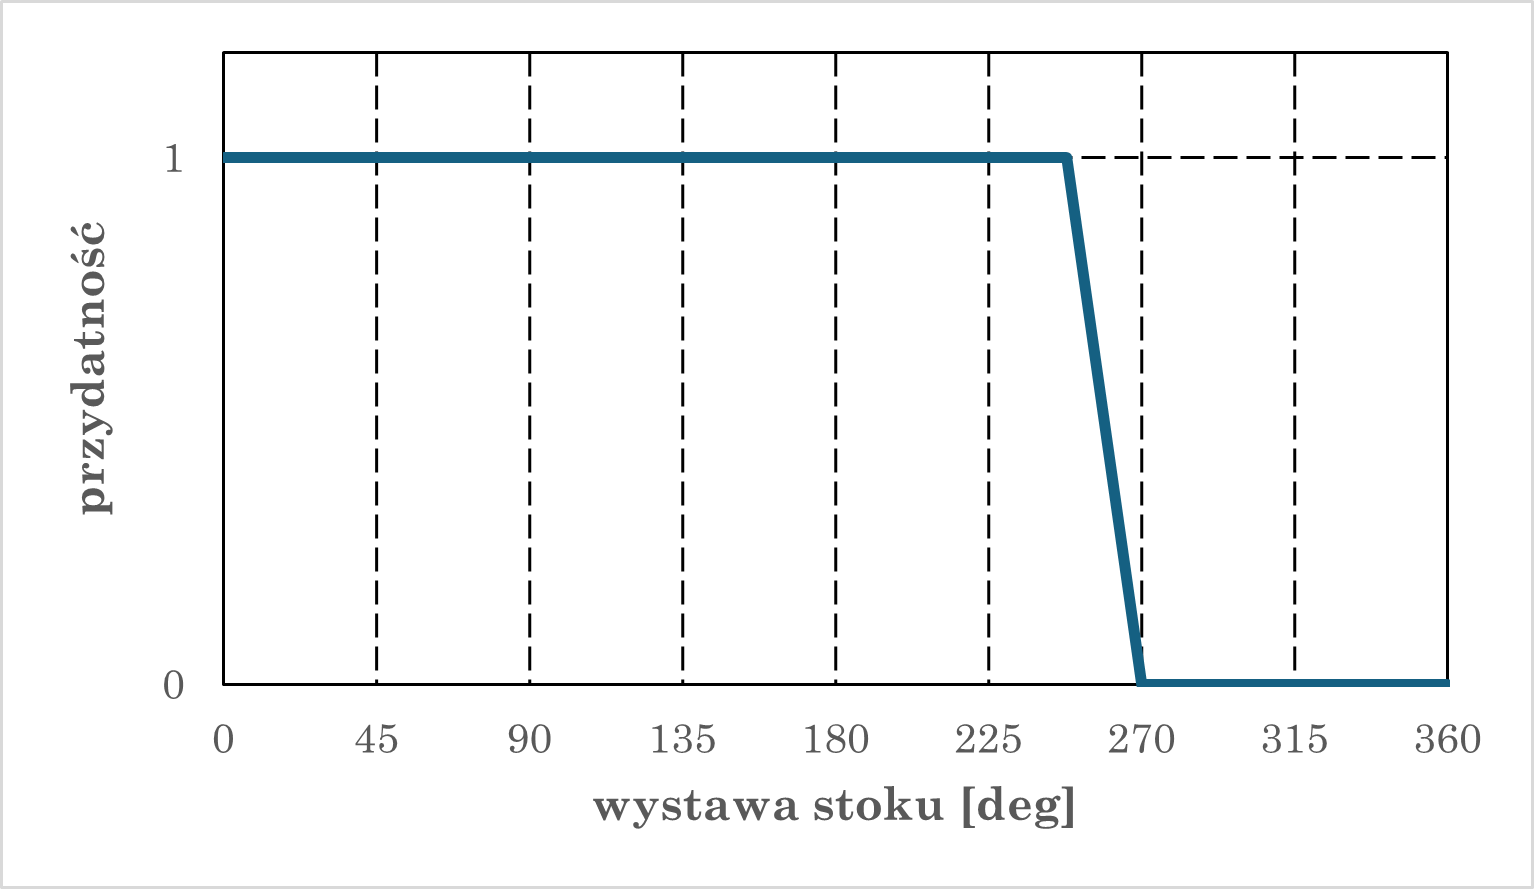
\includegraphics[width=\linewidth]{img/kryterium6-wykres-drugi.png}
        \caption*{}
    \end{minipage}
\end{figure}

\begin{figure}[H]
    \centering
    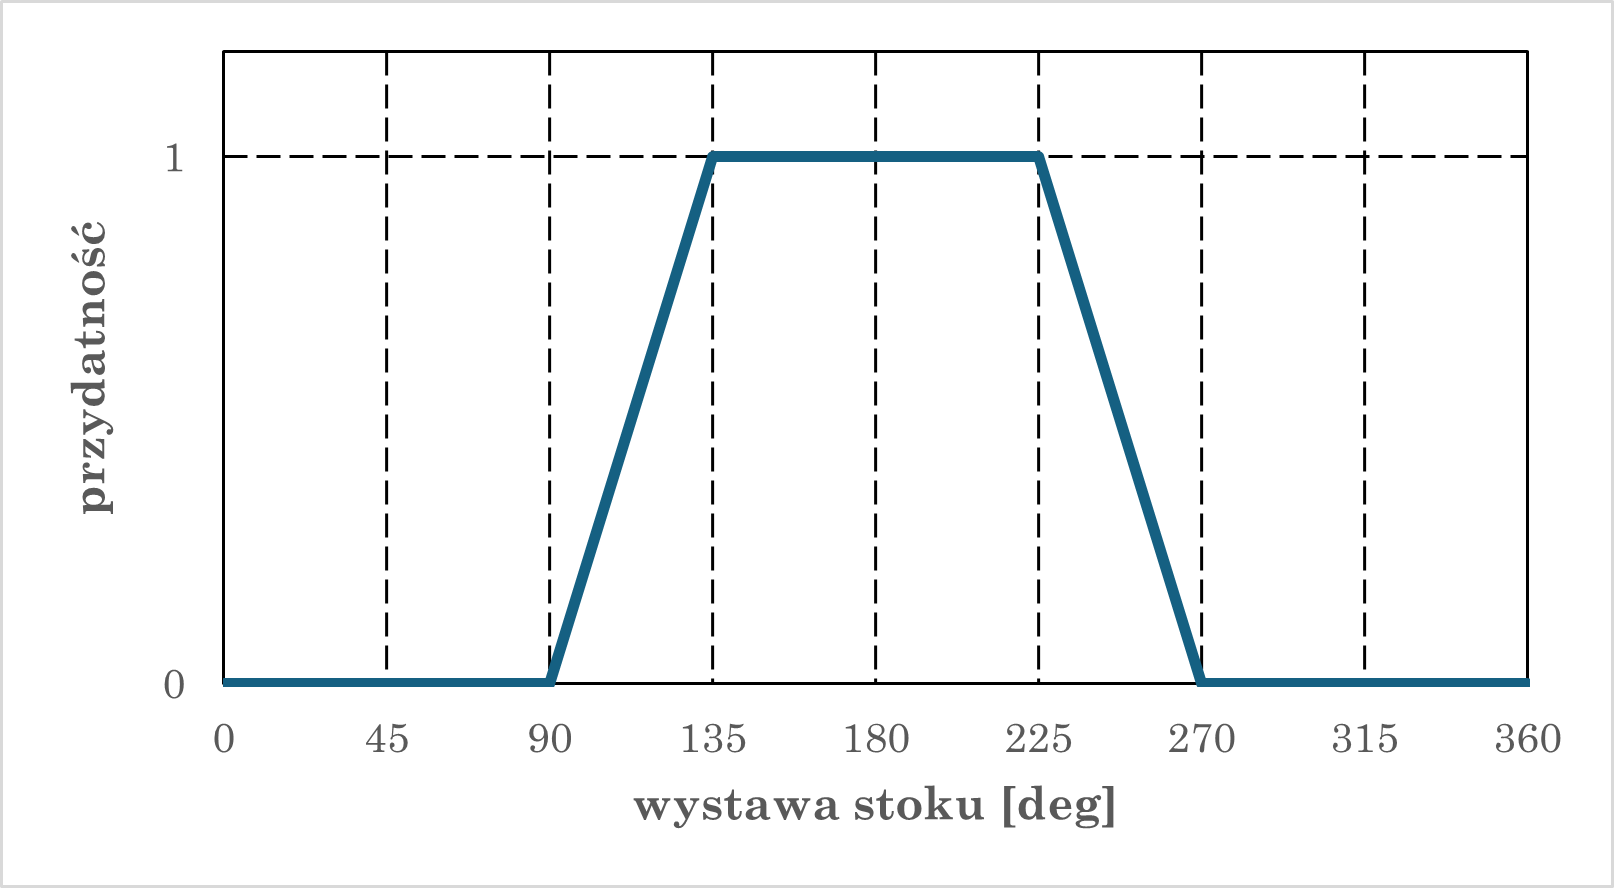
\includegraphics[width=0.75\textwidth]{img/kryterium6-wykres-glowny.png}
    \caption*{Reklasyfikacja dla kryterium 6.}
\end{figure}


\subsubsection{Kod}
\begin{lstlisting}
aspect = arcpy.ddd.Aspect(nmt)
aspect_fuzzy = arcpy.sa.FuzzyMembership(aspect, fuzzy_function="LINEAR 90 135")
aspect_fuzzy_1 = arcpy.sa.FuzzyMembership(aspect, fuzzy_function="LINEAR 270 225")
aspect_overlay = arcpy.sa.FuzzyOverlay([aspect_fuzzy, aspect_fuzzy_1], 'AND')
aspect_overlay.save(f'{geobaza}\\kryterium_6')
\end{lstlisting}

\subsubsection{Wynik}
\begin{figure}[H]
    \centering
    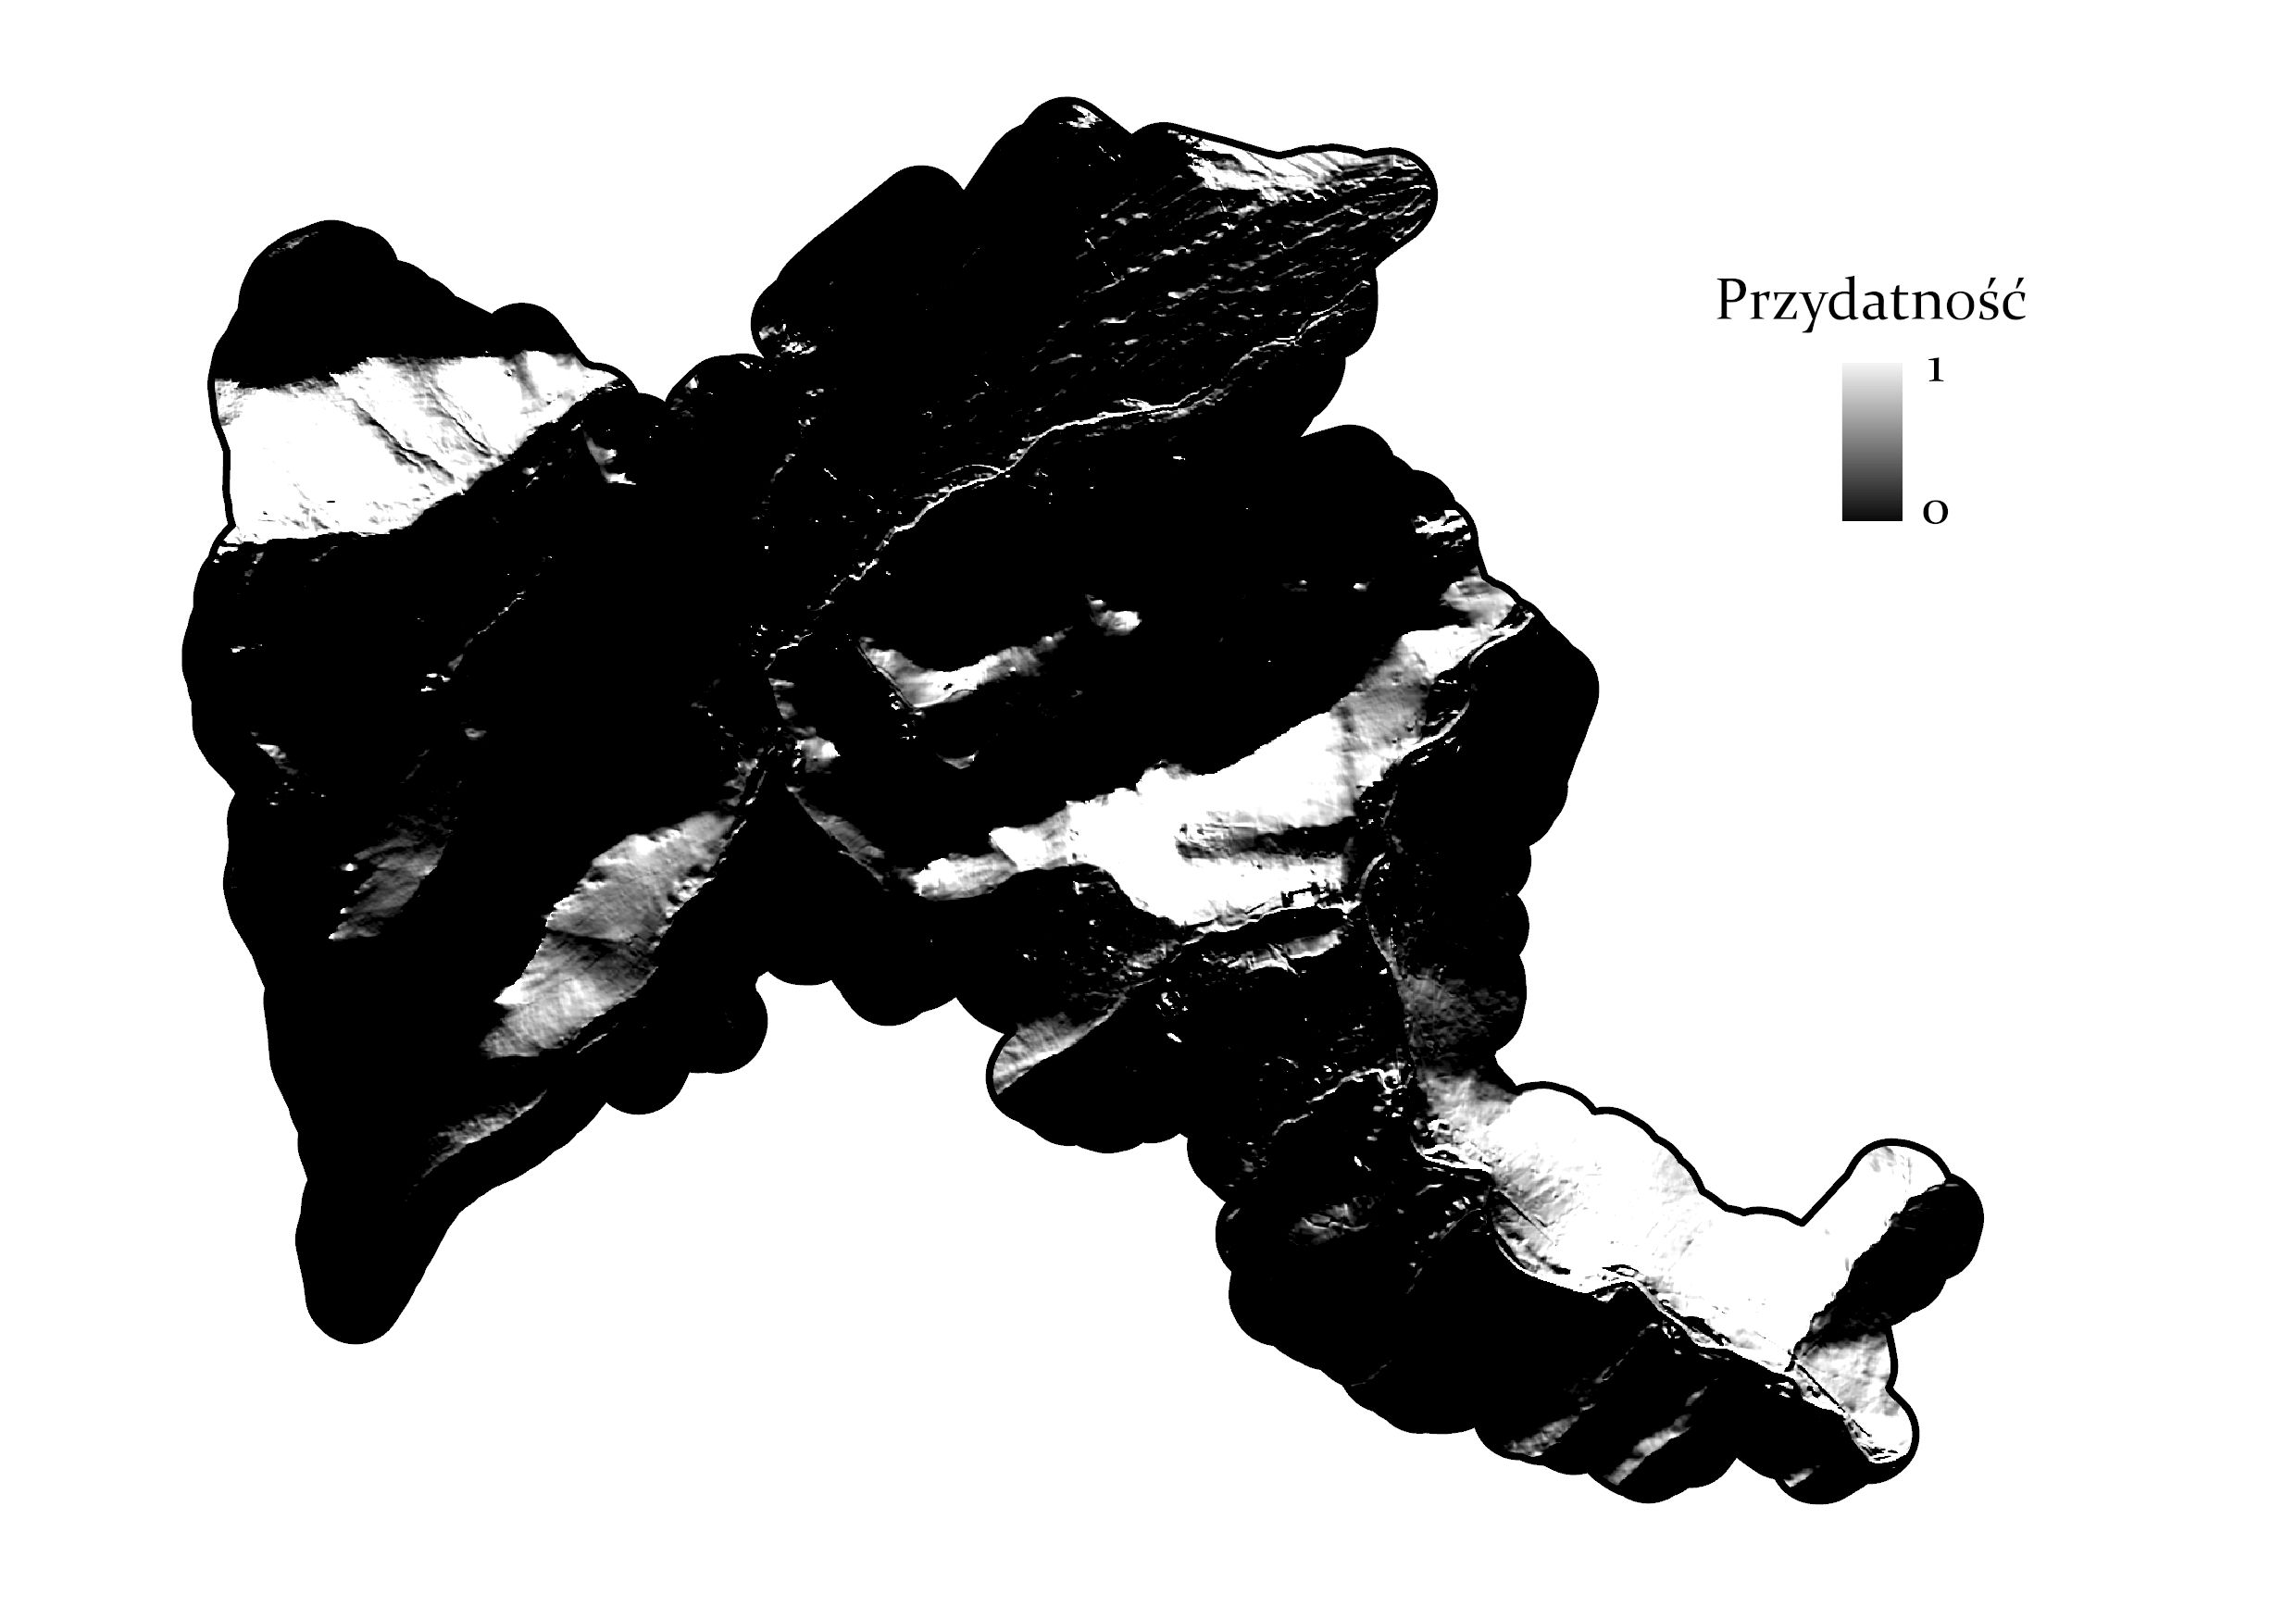
\includegraphics[width=0.75\textwidth]{img/kryterium6-layout.jpg}
    \caption*{Mapa przydatności dla kryterium 6.}
\end{figure}

\begin{figure}[H]
    \centering
    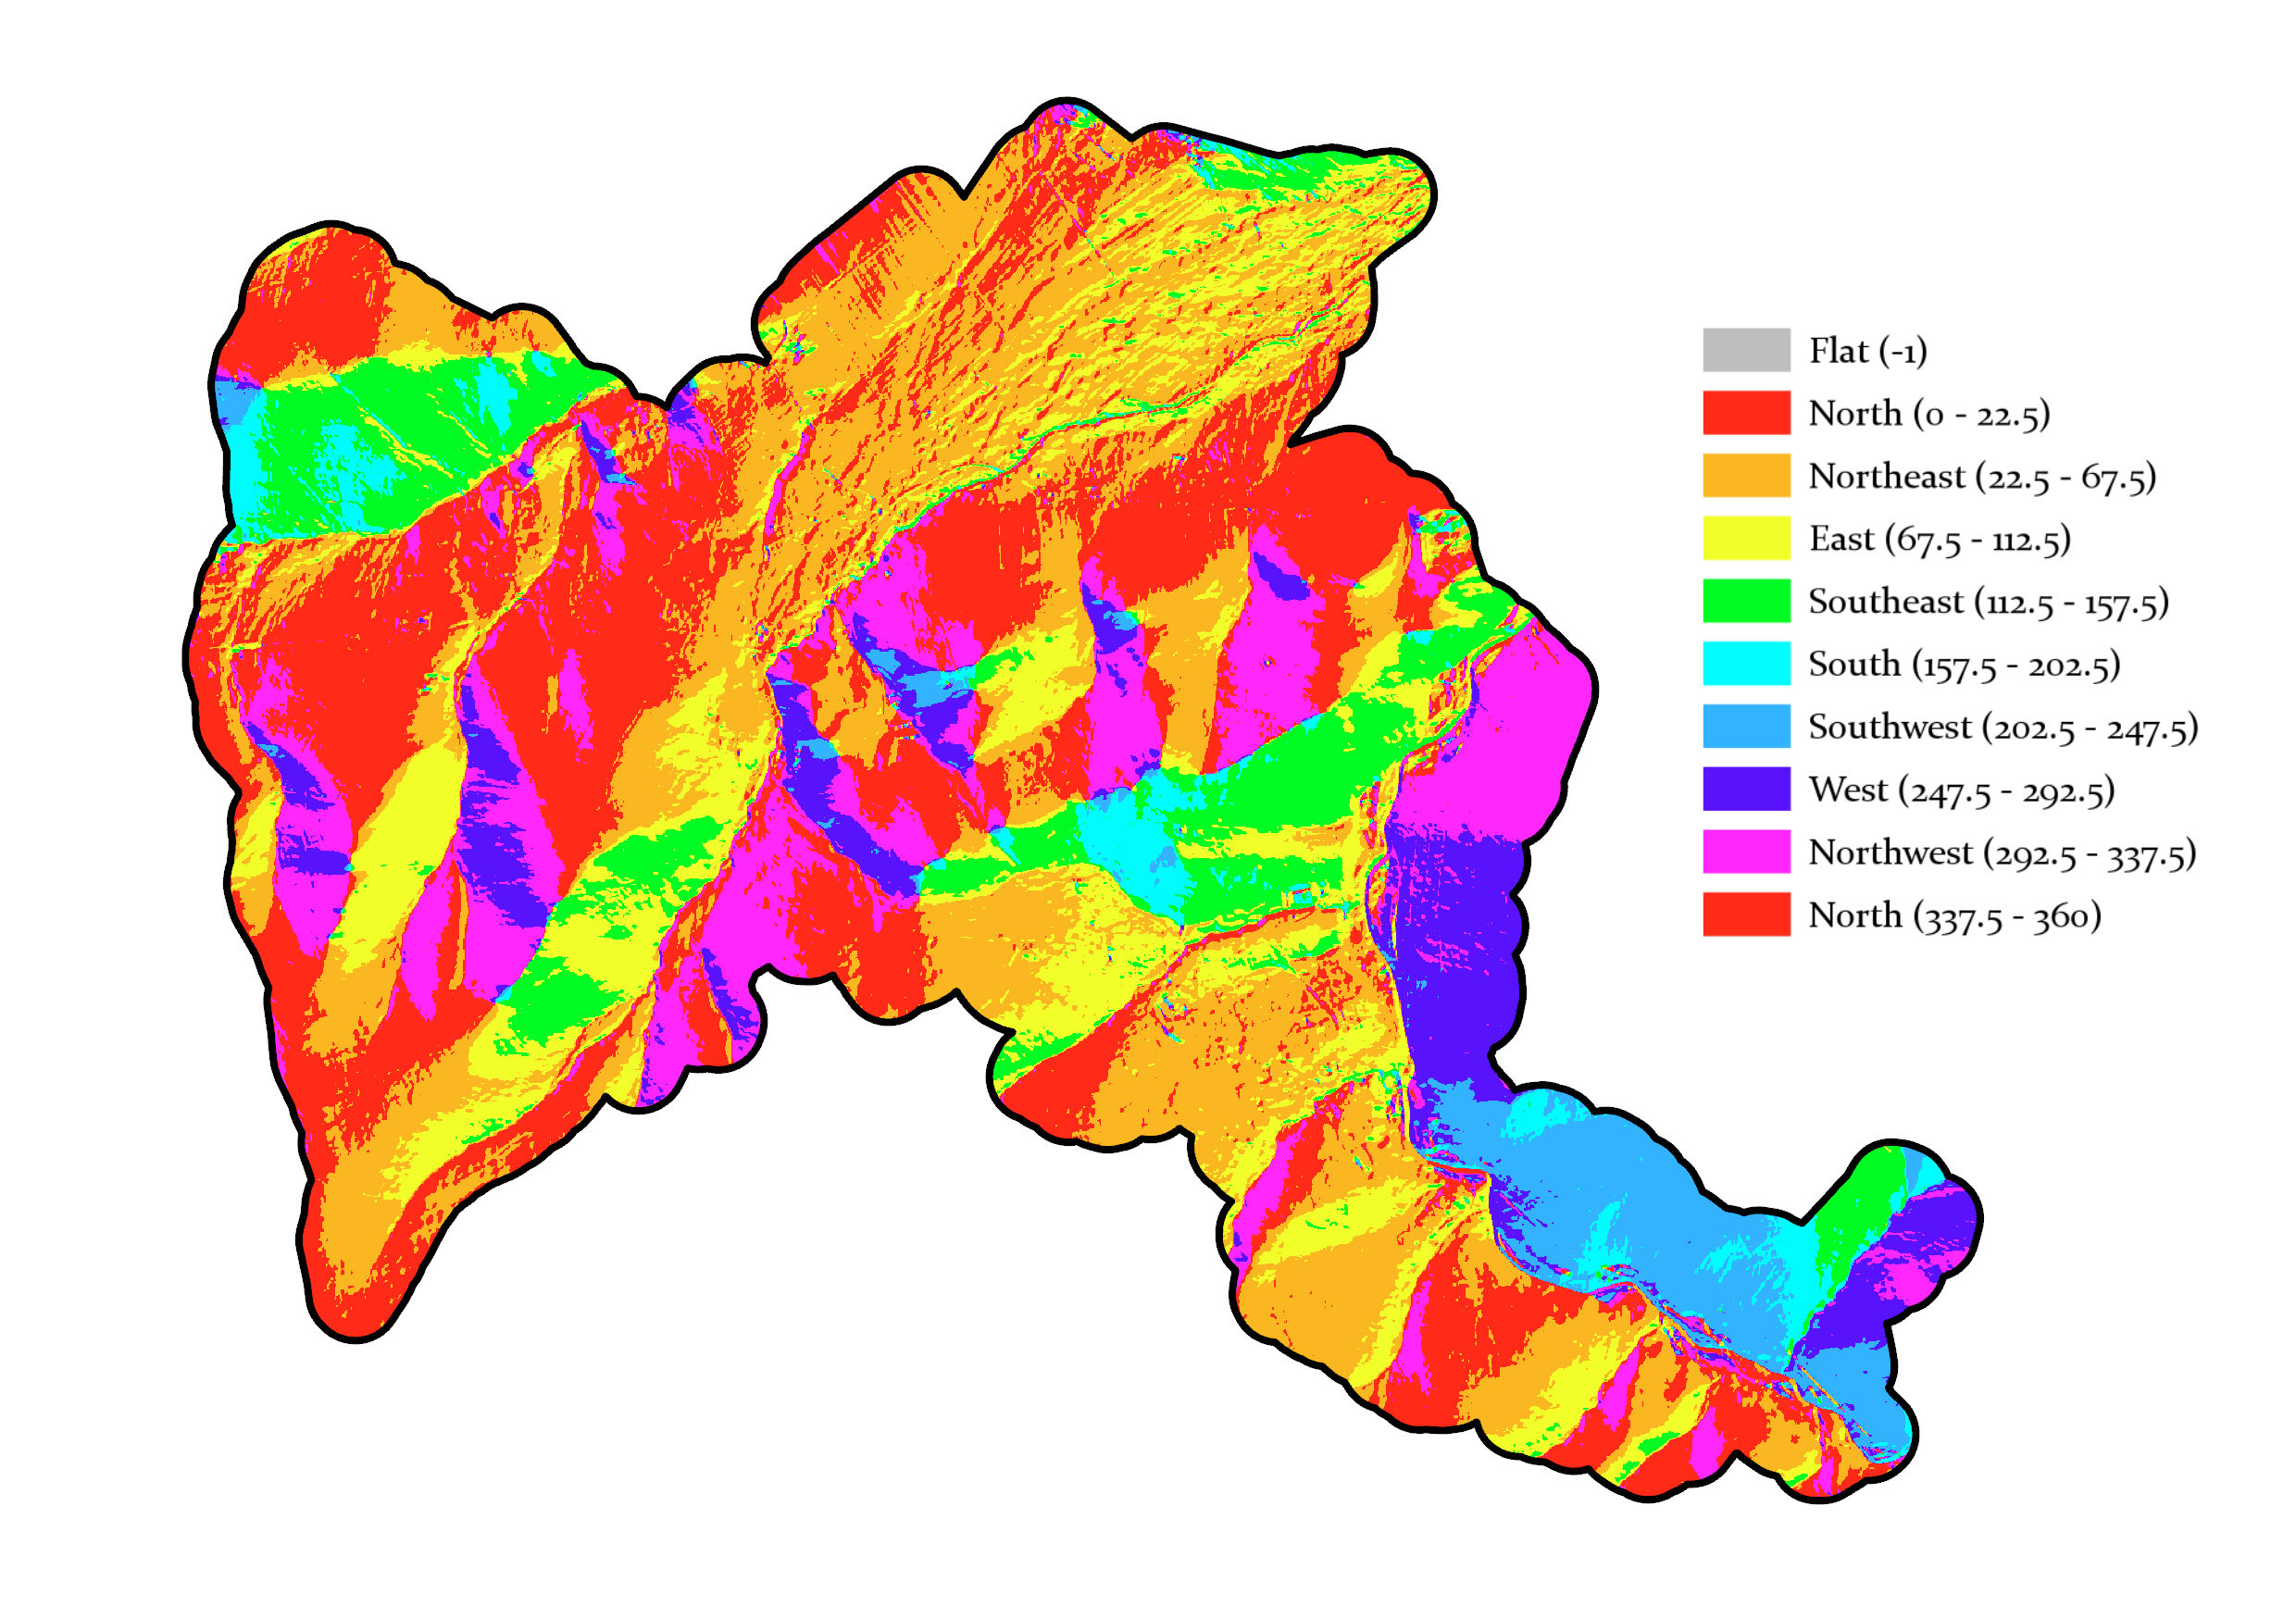
\includegraphics[width=0.75\textwidth]{img/kryterium6-aspect.jpg}
    \caption*{Mapa przydatności dla kryterium 6. zawierająca stopień wystawy słonecznej}
\end{figure}


\newpage
\subsection{Kryterium 7: dojazd do istotnych drogowych węzłów komunikacyjnych}
\subsubsection{Opis działania}
\begin{figure}[H]
    \centering
    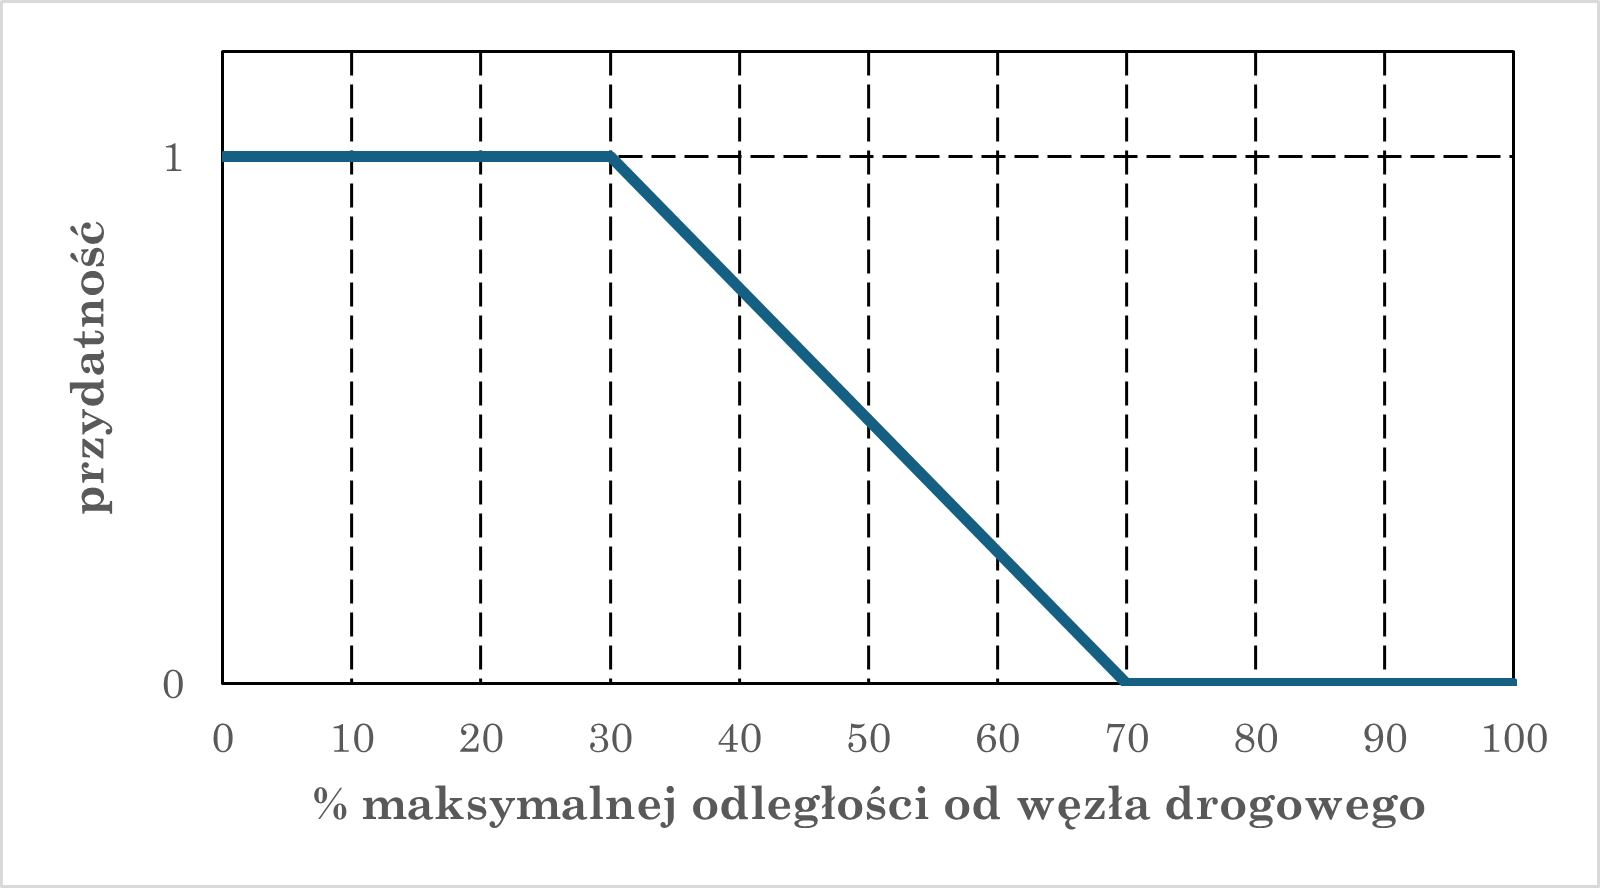
\includegraphics[width=0.75\textwidth]{img/kryterium7-wykres-glowny.png}
    \caption*{Reklasyfikacja dla kryterium 7.}
\end{figure}


\subsubsection{Kod}
\begin{lstlisting}
wezly_max = float(arcpy.management.GetRasterProperties(wezly, "MAXIMUM")[0].replace(',', '.'))
wezly_fuzzy = arcpy.sa.FuzzyMembership(wezly, fuzzy_function=f"LINEAR {0.7 * wezly_max} {0.3 * wezly_max}")
wezly_fuzzy.save(f'{geobaza}\\kryterium_7')
\end{lstlisting}

\subsubsection{Wynik}

\begin{figure}[H]
    \centering
    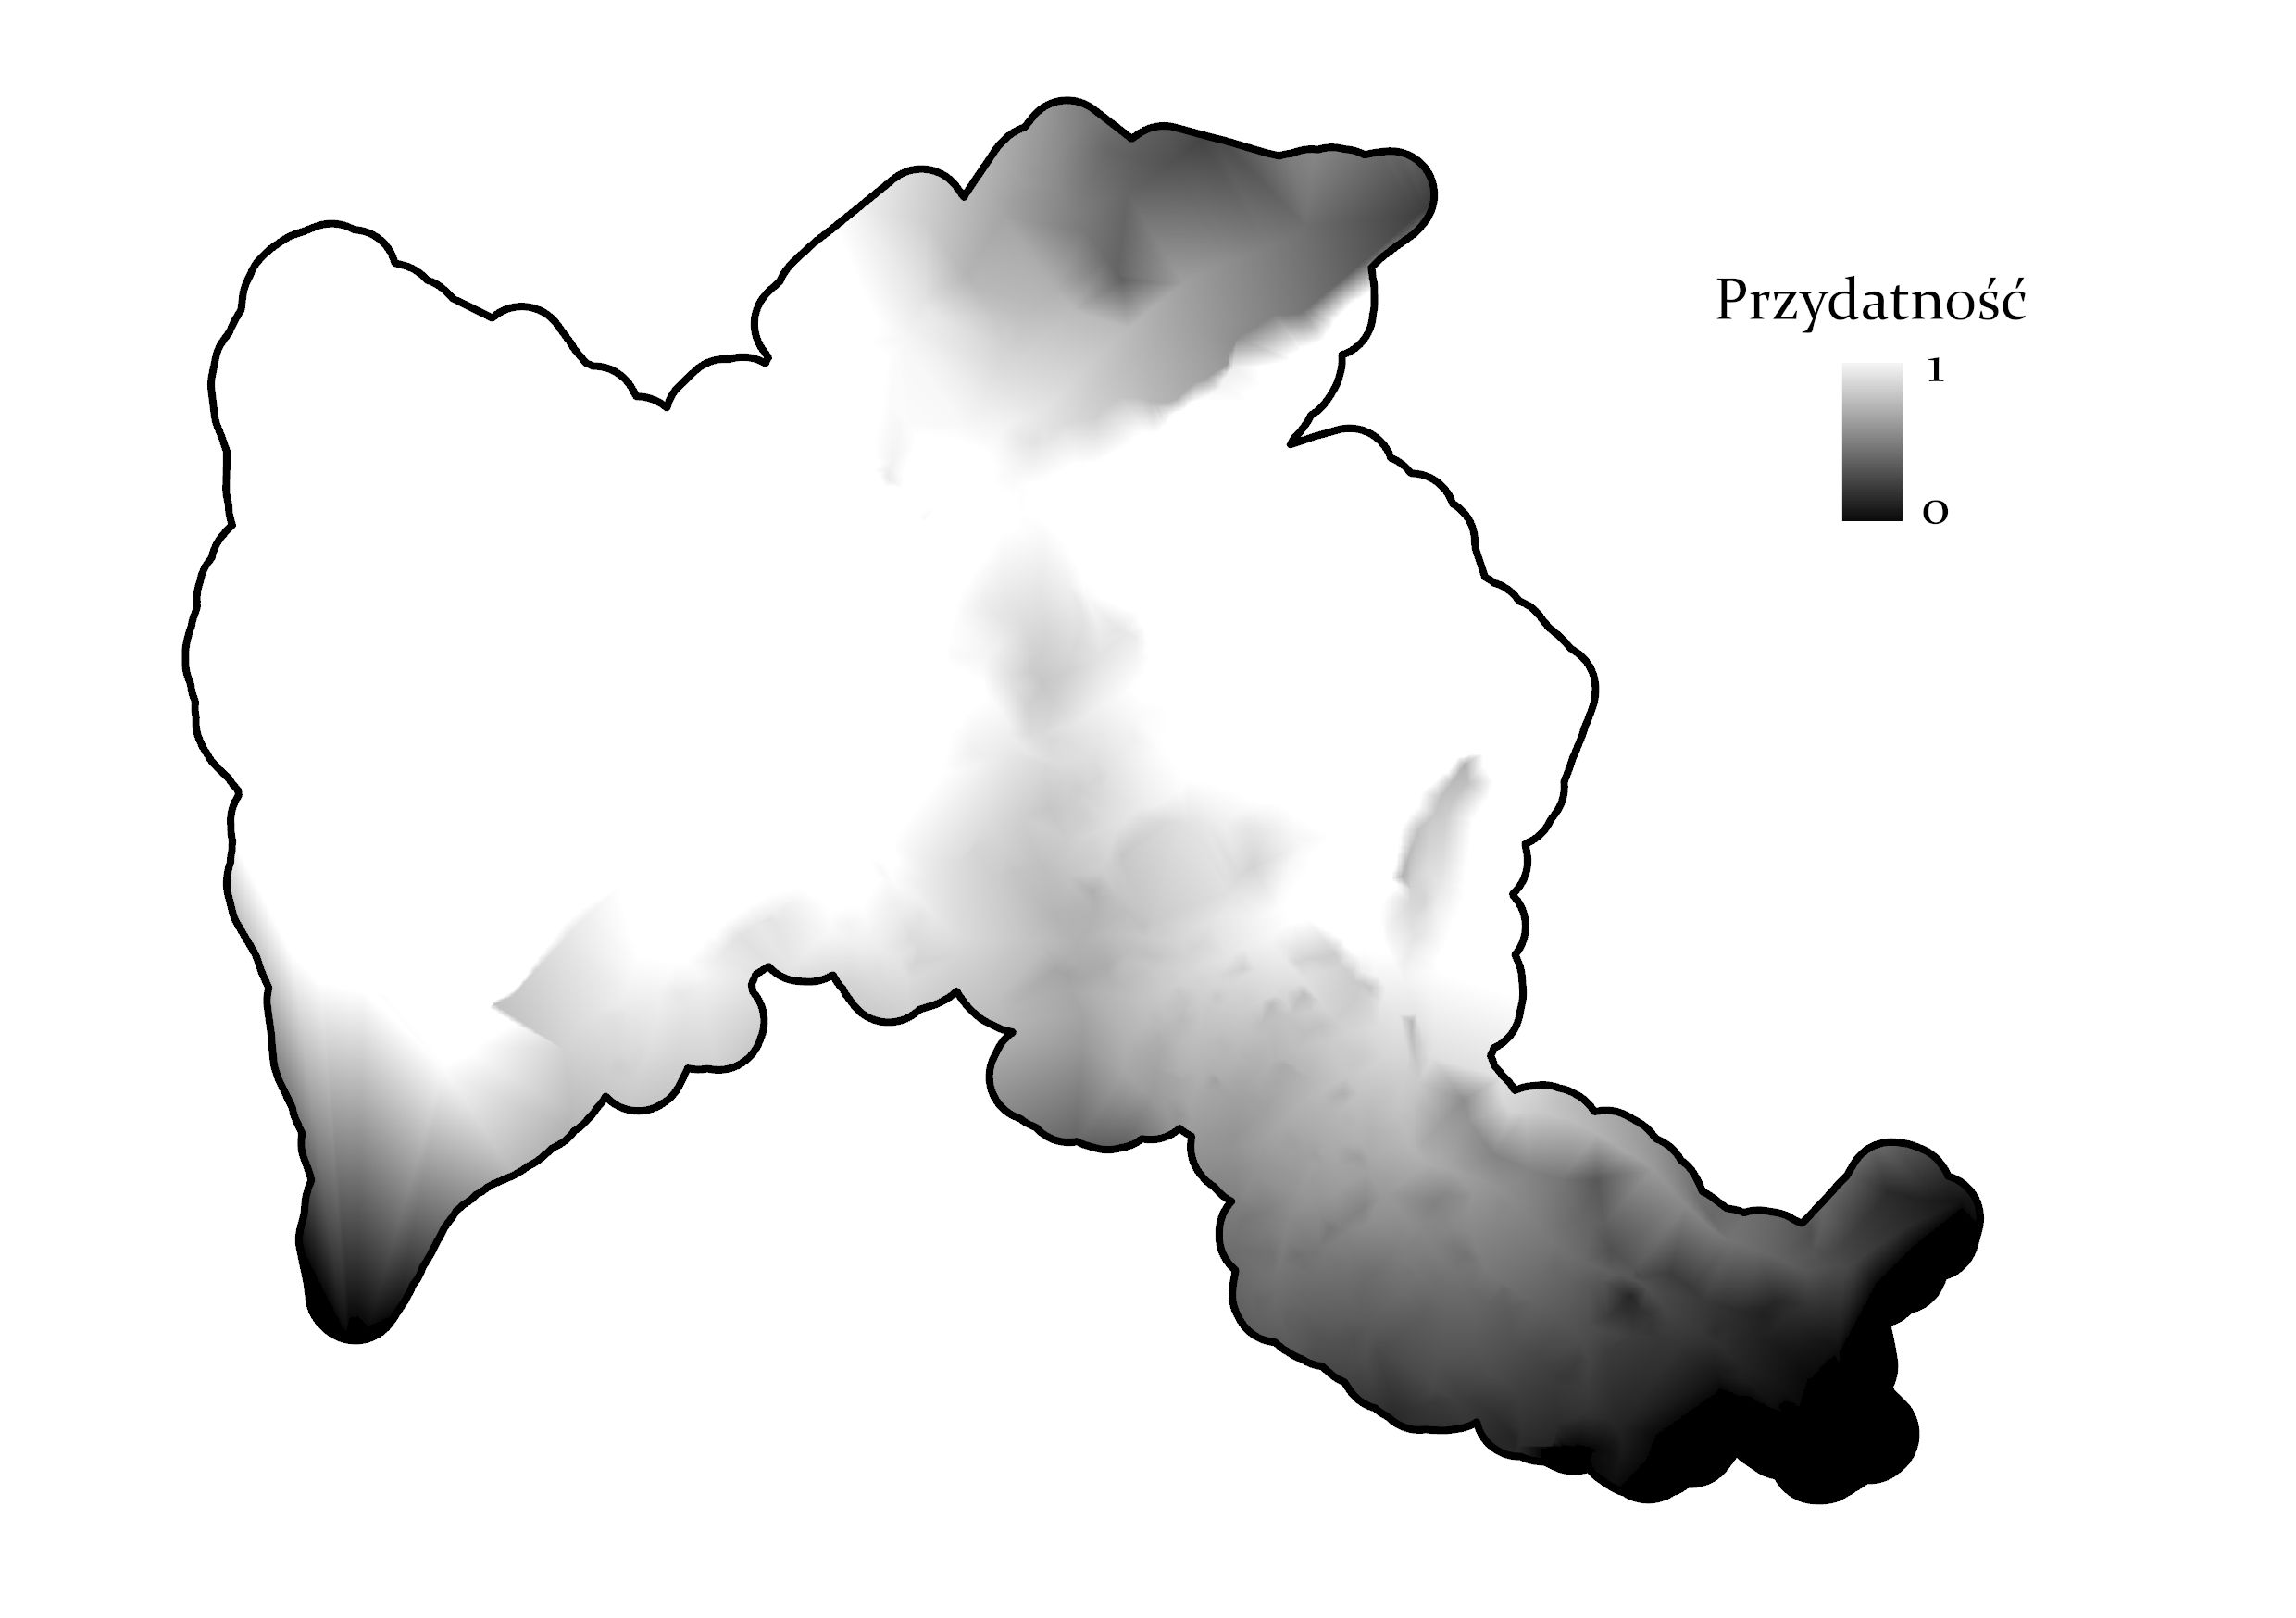
\includegraphics[width=0.75\textwidth]{img/kryterium7-layout.jpg}
    \caption*{Mapa przydatności dla kryterium 7.}
\end{figure}

\begin{figure}[H]
    \centering
    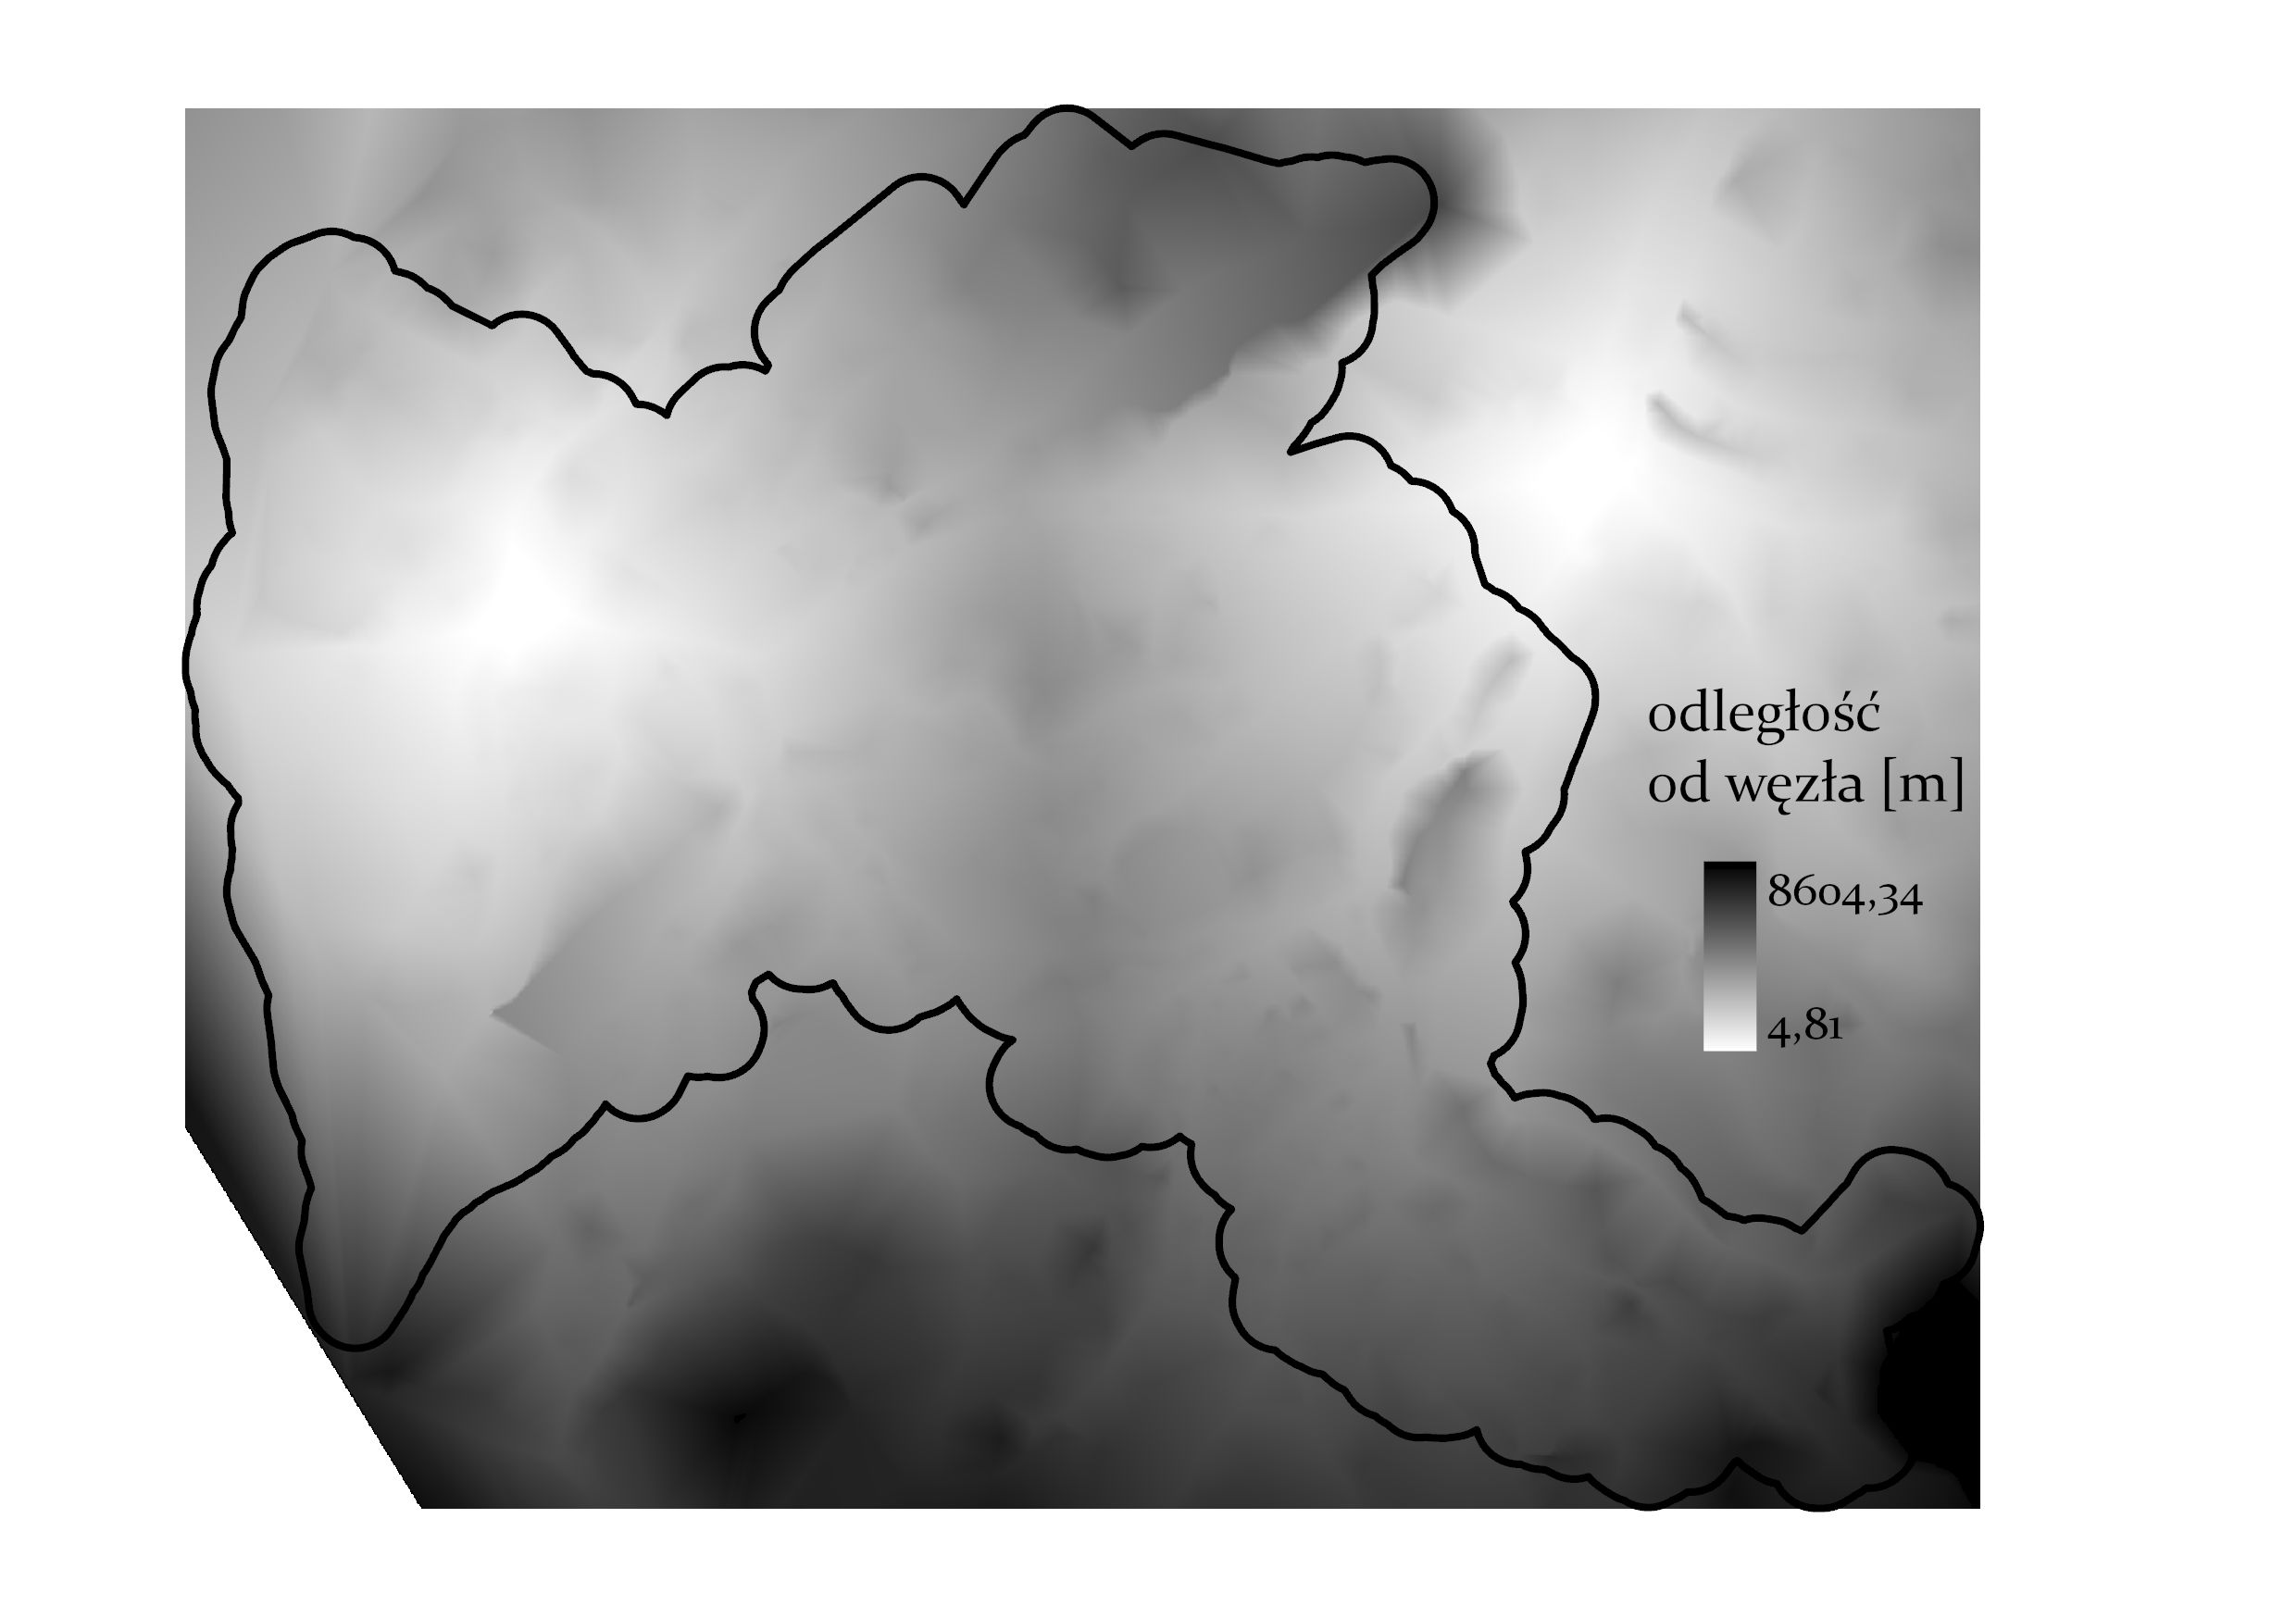
\includegraphics[width=0.75\textwidth]{img/kryterium7-wezly.jpg}
    \caption*{Mapa odległości od węzłów}
\end{figure}

\subsection{Ocena przydatności terenu}
\subsubsection{Opis działania}
Powyższy kod najpierw tworzy tabelę zawierającą wagi dla każdego z kryteriów, zmienne w zależności od wariantu. Następnie tworzy sumę ważoną dla wszystkich z kryteriów.

Później brane są pod uwagę kryteria ostre, tj. 100-metrowa strefa ochronna od wód, 150-metrowa odległość od budynków mieszkalnych oraz 15-metrowa odległość od lasów. Zostaje utworzony raster, który w pikselu, dla którego przydatność dla któregokolwiek z kryterium wyniosła 0, przyjmuje również przydatność równą 0. Dzięki temu miejsca wyeliminowane przez którekolwiek z kryteriów ostrych nie będą brane pod uwagę przy wyborze lokalizacji farmy. 

Następnie zostaje utworzona suma warstwy kryteriów ostrych i rozmytych. Piksele z przydatnością powyżej progu przydatności zostały zremapowane na 1, pozostałe na 0.

\subsubsection{Kod}
\begin{lstlisting}
tabela_kryteriow = arcpy.sa.WSTable([[f'{geobaza}\\kryterium_1', "VALUE", waga_woda], [f'{geobaza}\\kryterium_2', "VALUE", waga_budynki], [f'{geobaza}\\kryterium_3', "VALUE", waga_lasy], [f'{geobaza}\\kryterium_4', "VALUE", waga_drogi], [f'{geobaza}\\kryterium_5', "VALUE", waga_wysokosc], [f'{geobaza}\\kryterium_6', "VALUE", waga_aspect], [f'{geobaza}\\kryterium_7', "VALUE", waga_wezly]])
weighted_sum = arcpy.sa.WeightedSum(tabela_kryteriow)
weighted_sum.save(f'{geobaza}\\{wariant}_suma_rozmyte')

kryteria_ostre = arcpy.sa.FuzzyOverlay([woda_rosnaca, f"{geobaza}\\kryterium_2", f"{geobaza}\\kryterium_3"], 'AND')
kryteria_ostre.save(f'{geobaza}\\kryteria_ostre')

suma = arcpy.sa.FuzzyOverlay([kryteria_ostre, weighted_sum], 'AND')
suma.save(f'{geobaza}\\{wariant}_wynik')

wynik_reclassified = arcpy.sa.Reclassify(suma, "VALUE", arcpy.sa.RemapRange([[0, prog_przydatnosci, 0], [prog_przydatnosci, 1, 1]]))
wynik_reclassified.save(f'{geobaza}\\{wariant}_wynik_reclassified')
\end{lstlisting}

\subsubsection{Wynik}
\begin{figure}[H]
    \centering
    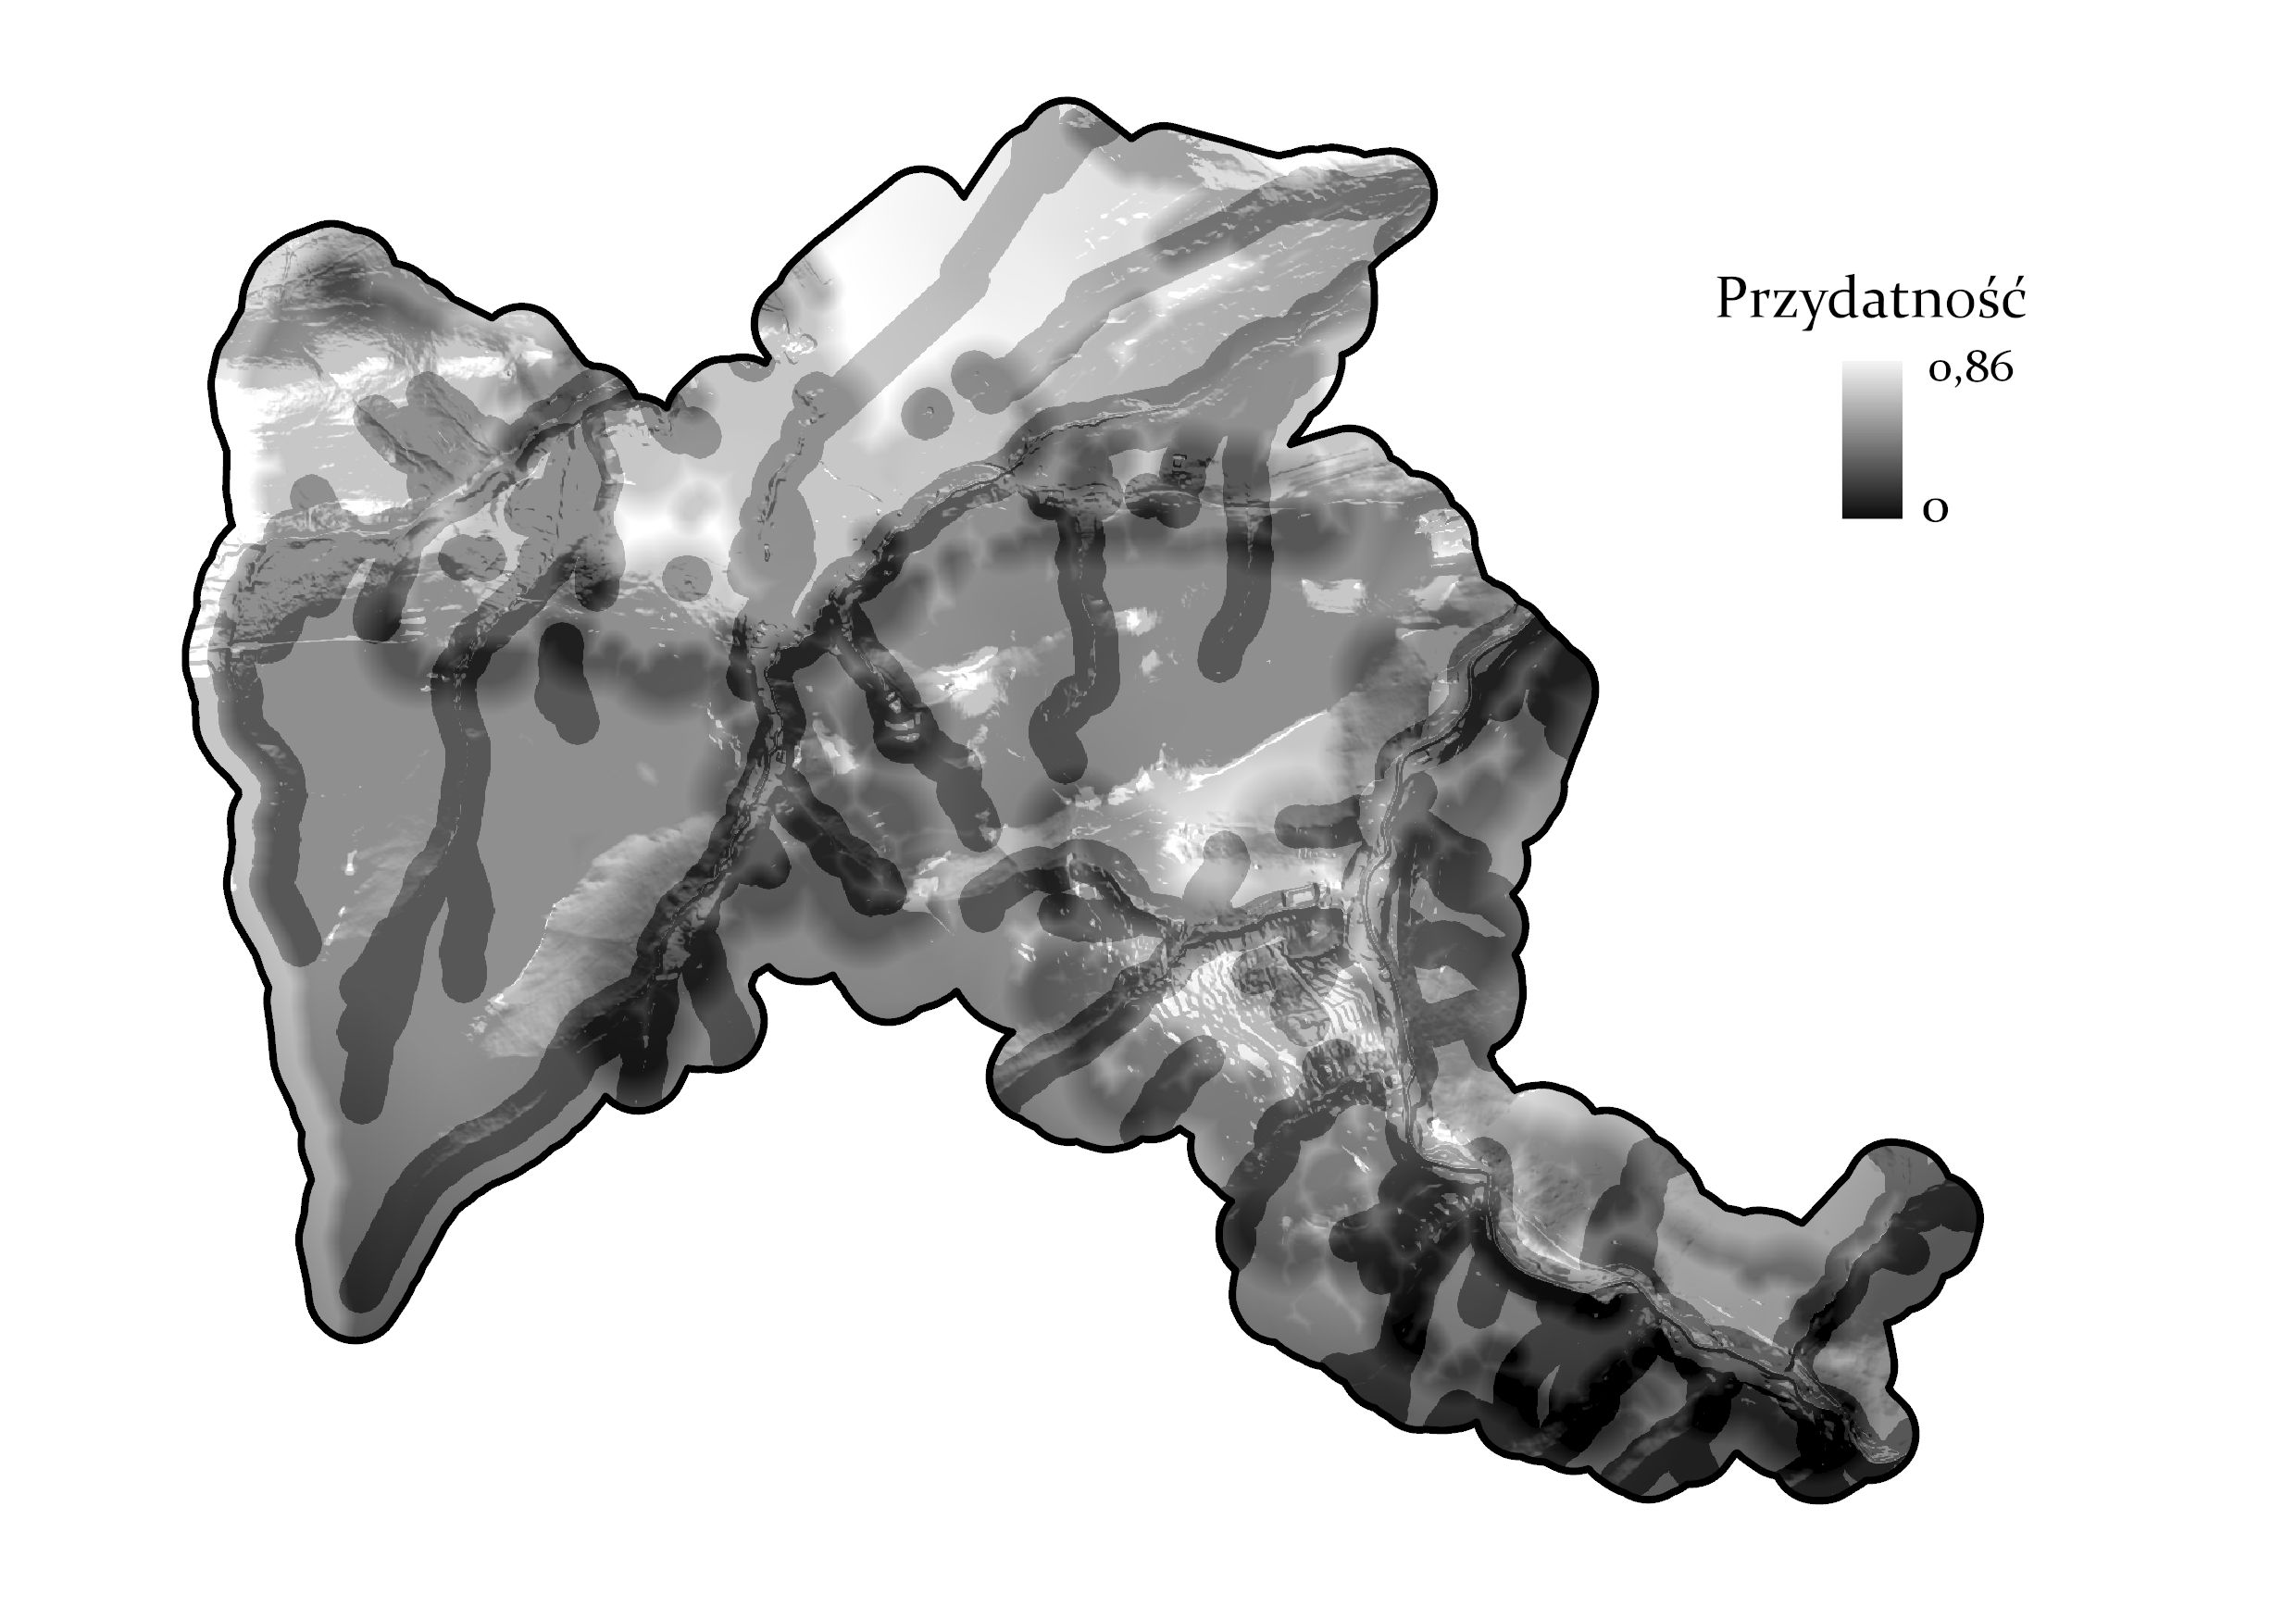
\includegraphics[width=0.75\textwidth]{img/rozmyte-layout.jpg}
    \caption*{Suma kryteriów rozmytych}
\end{figure}

\begin{figure}[H]
    \centering
    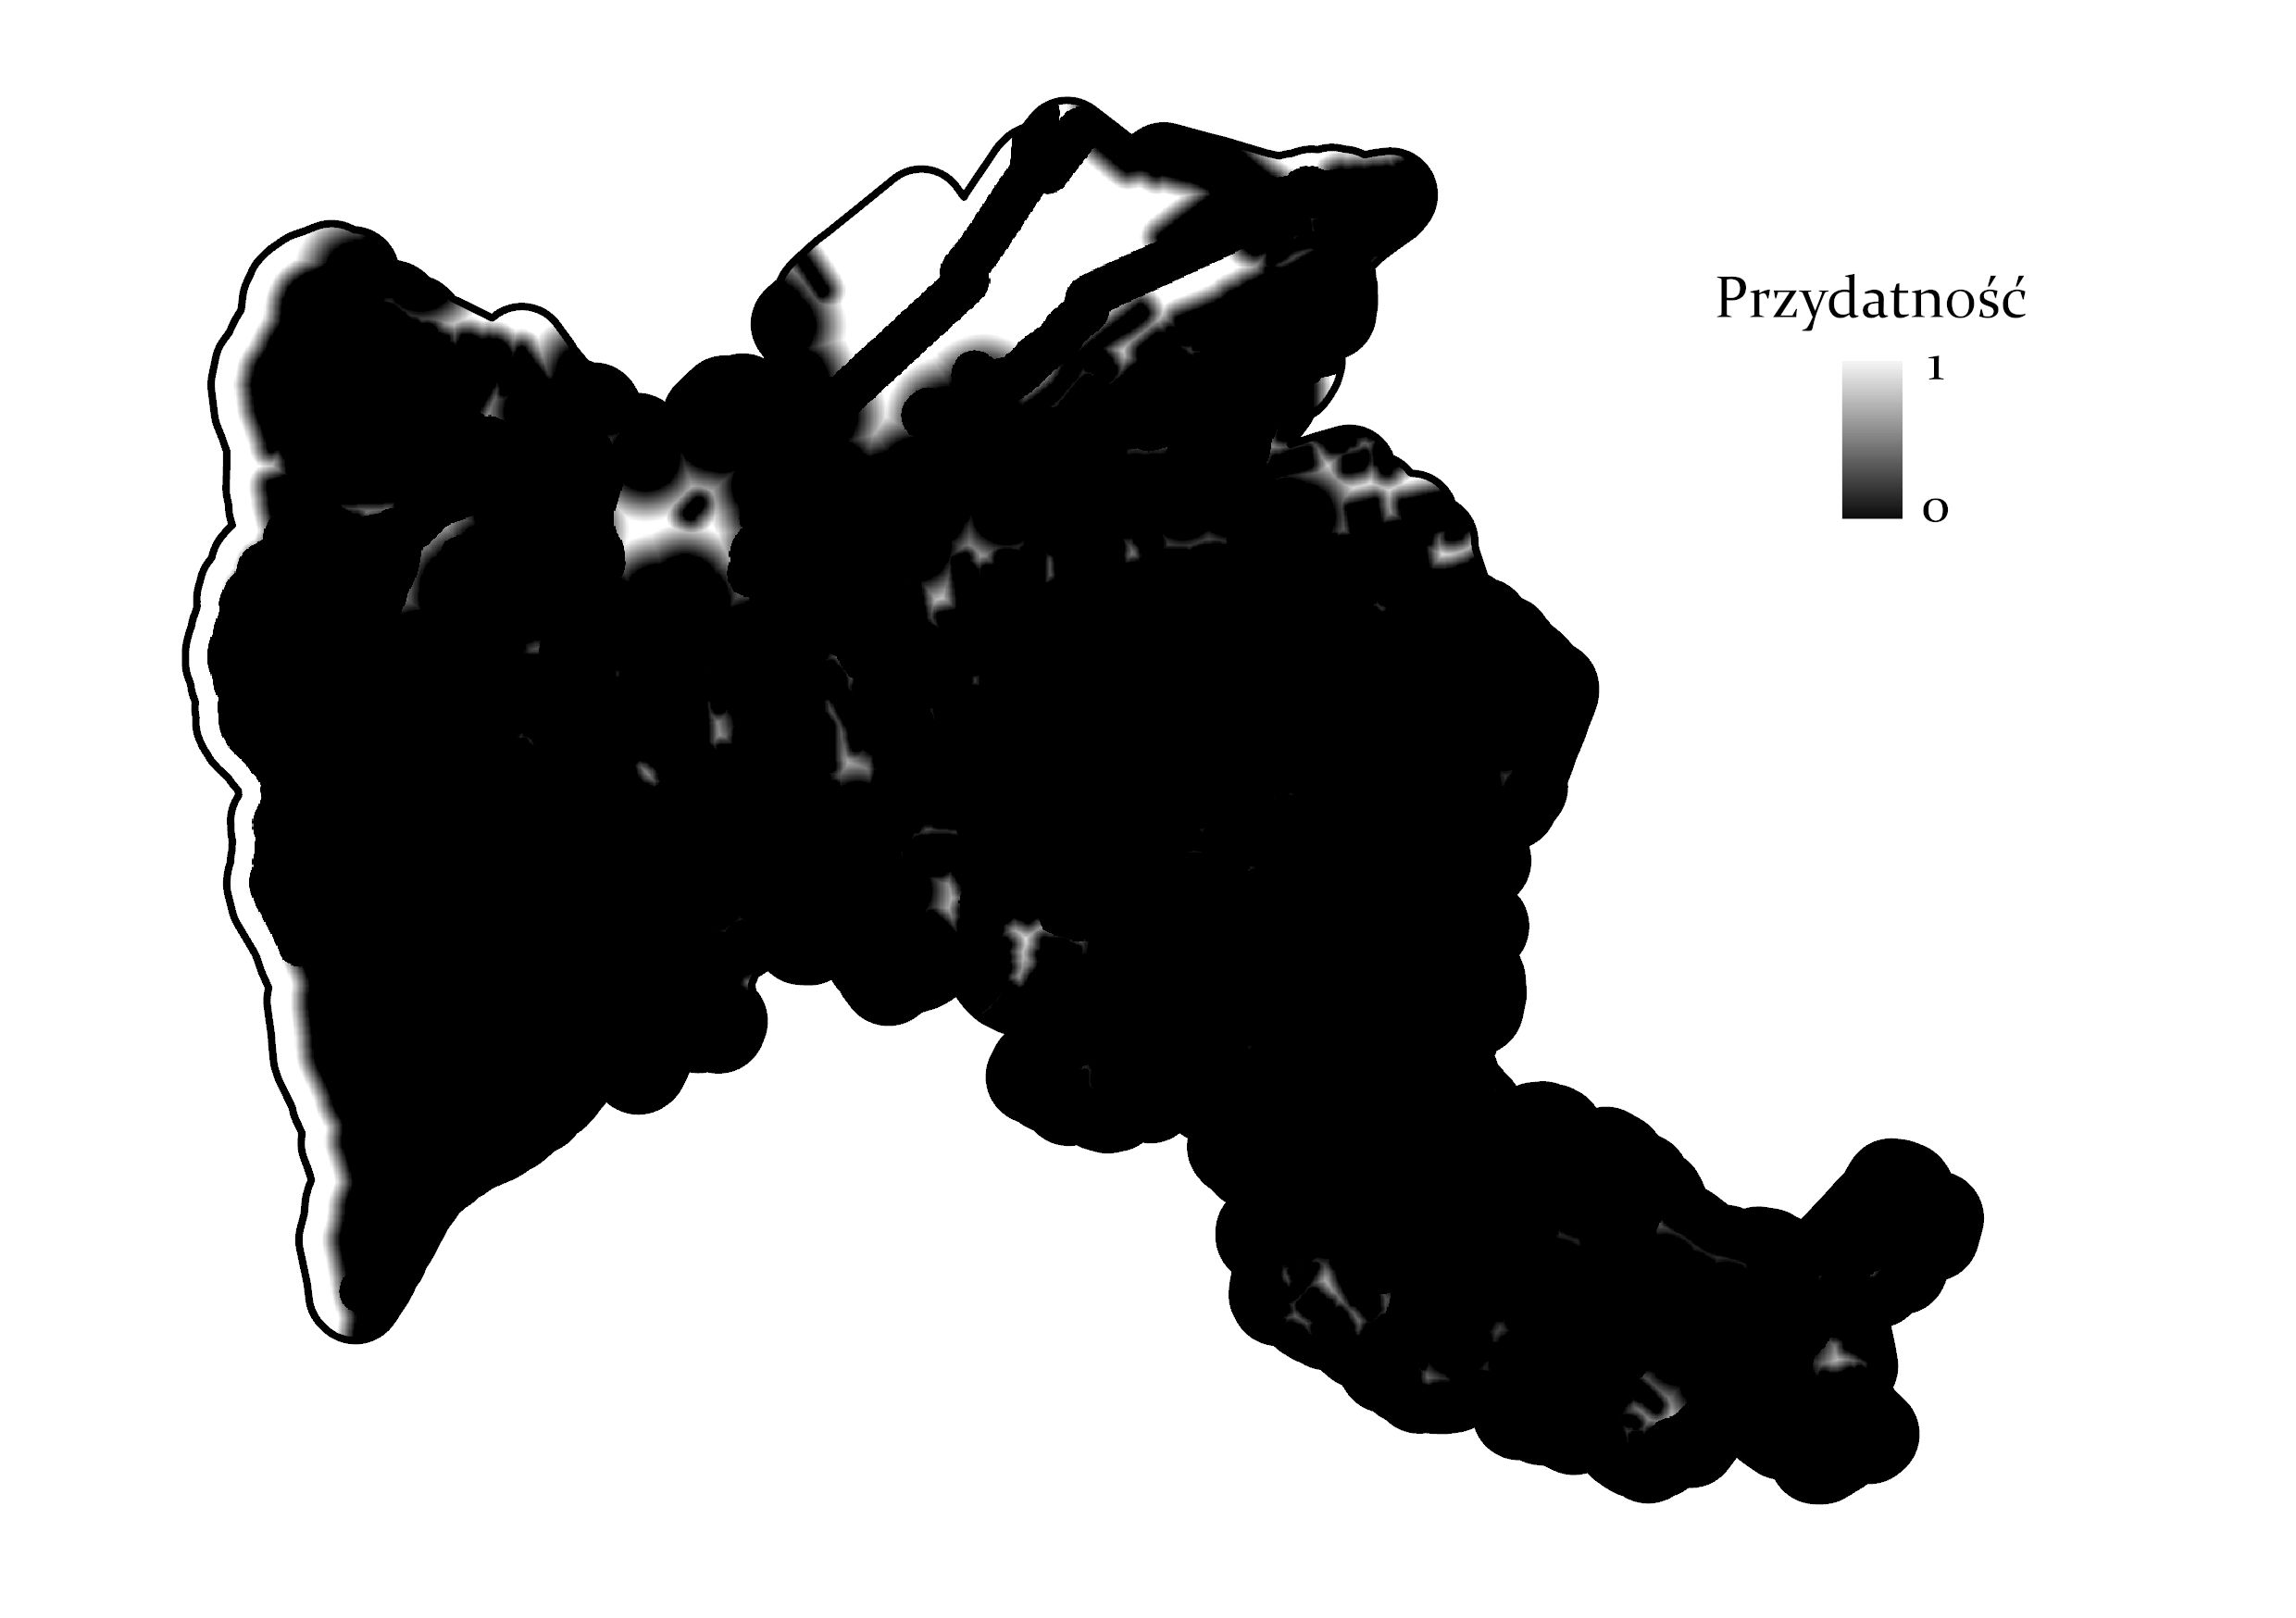
\includegraphics[width=0.75\textwidth]{img/ostre-layout.jpg}
    \caption*{Suma kryteriów ostrych}
\end{figure}

\begin{figure}[H]
    \centering
    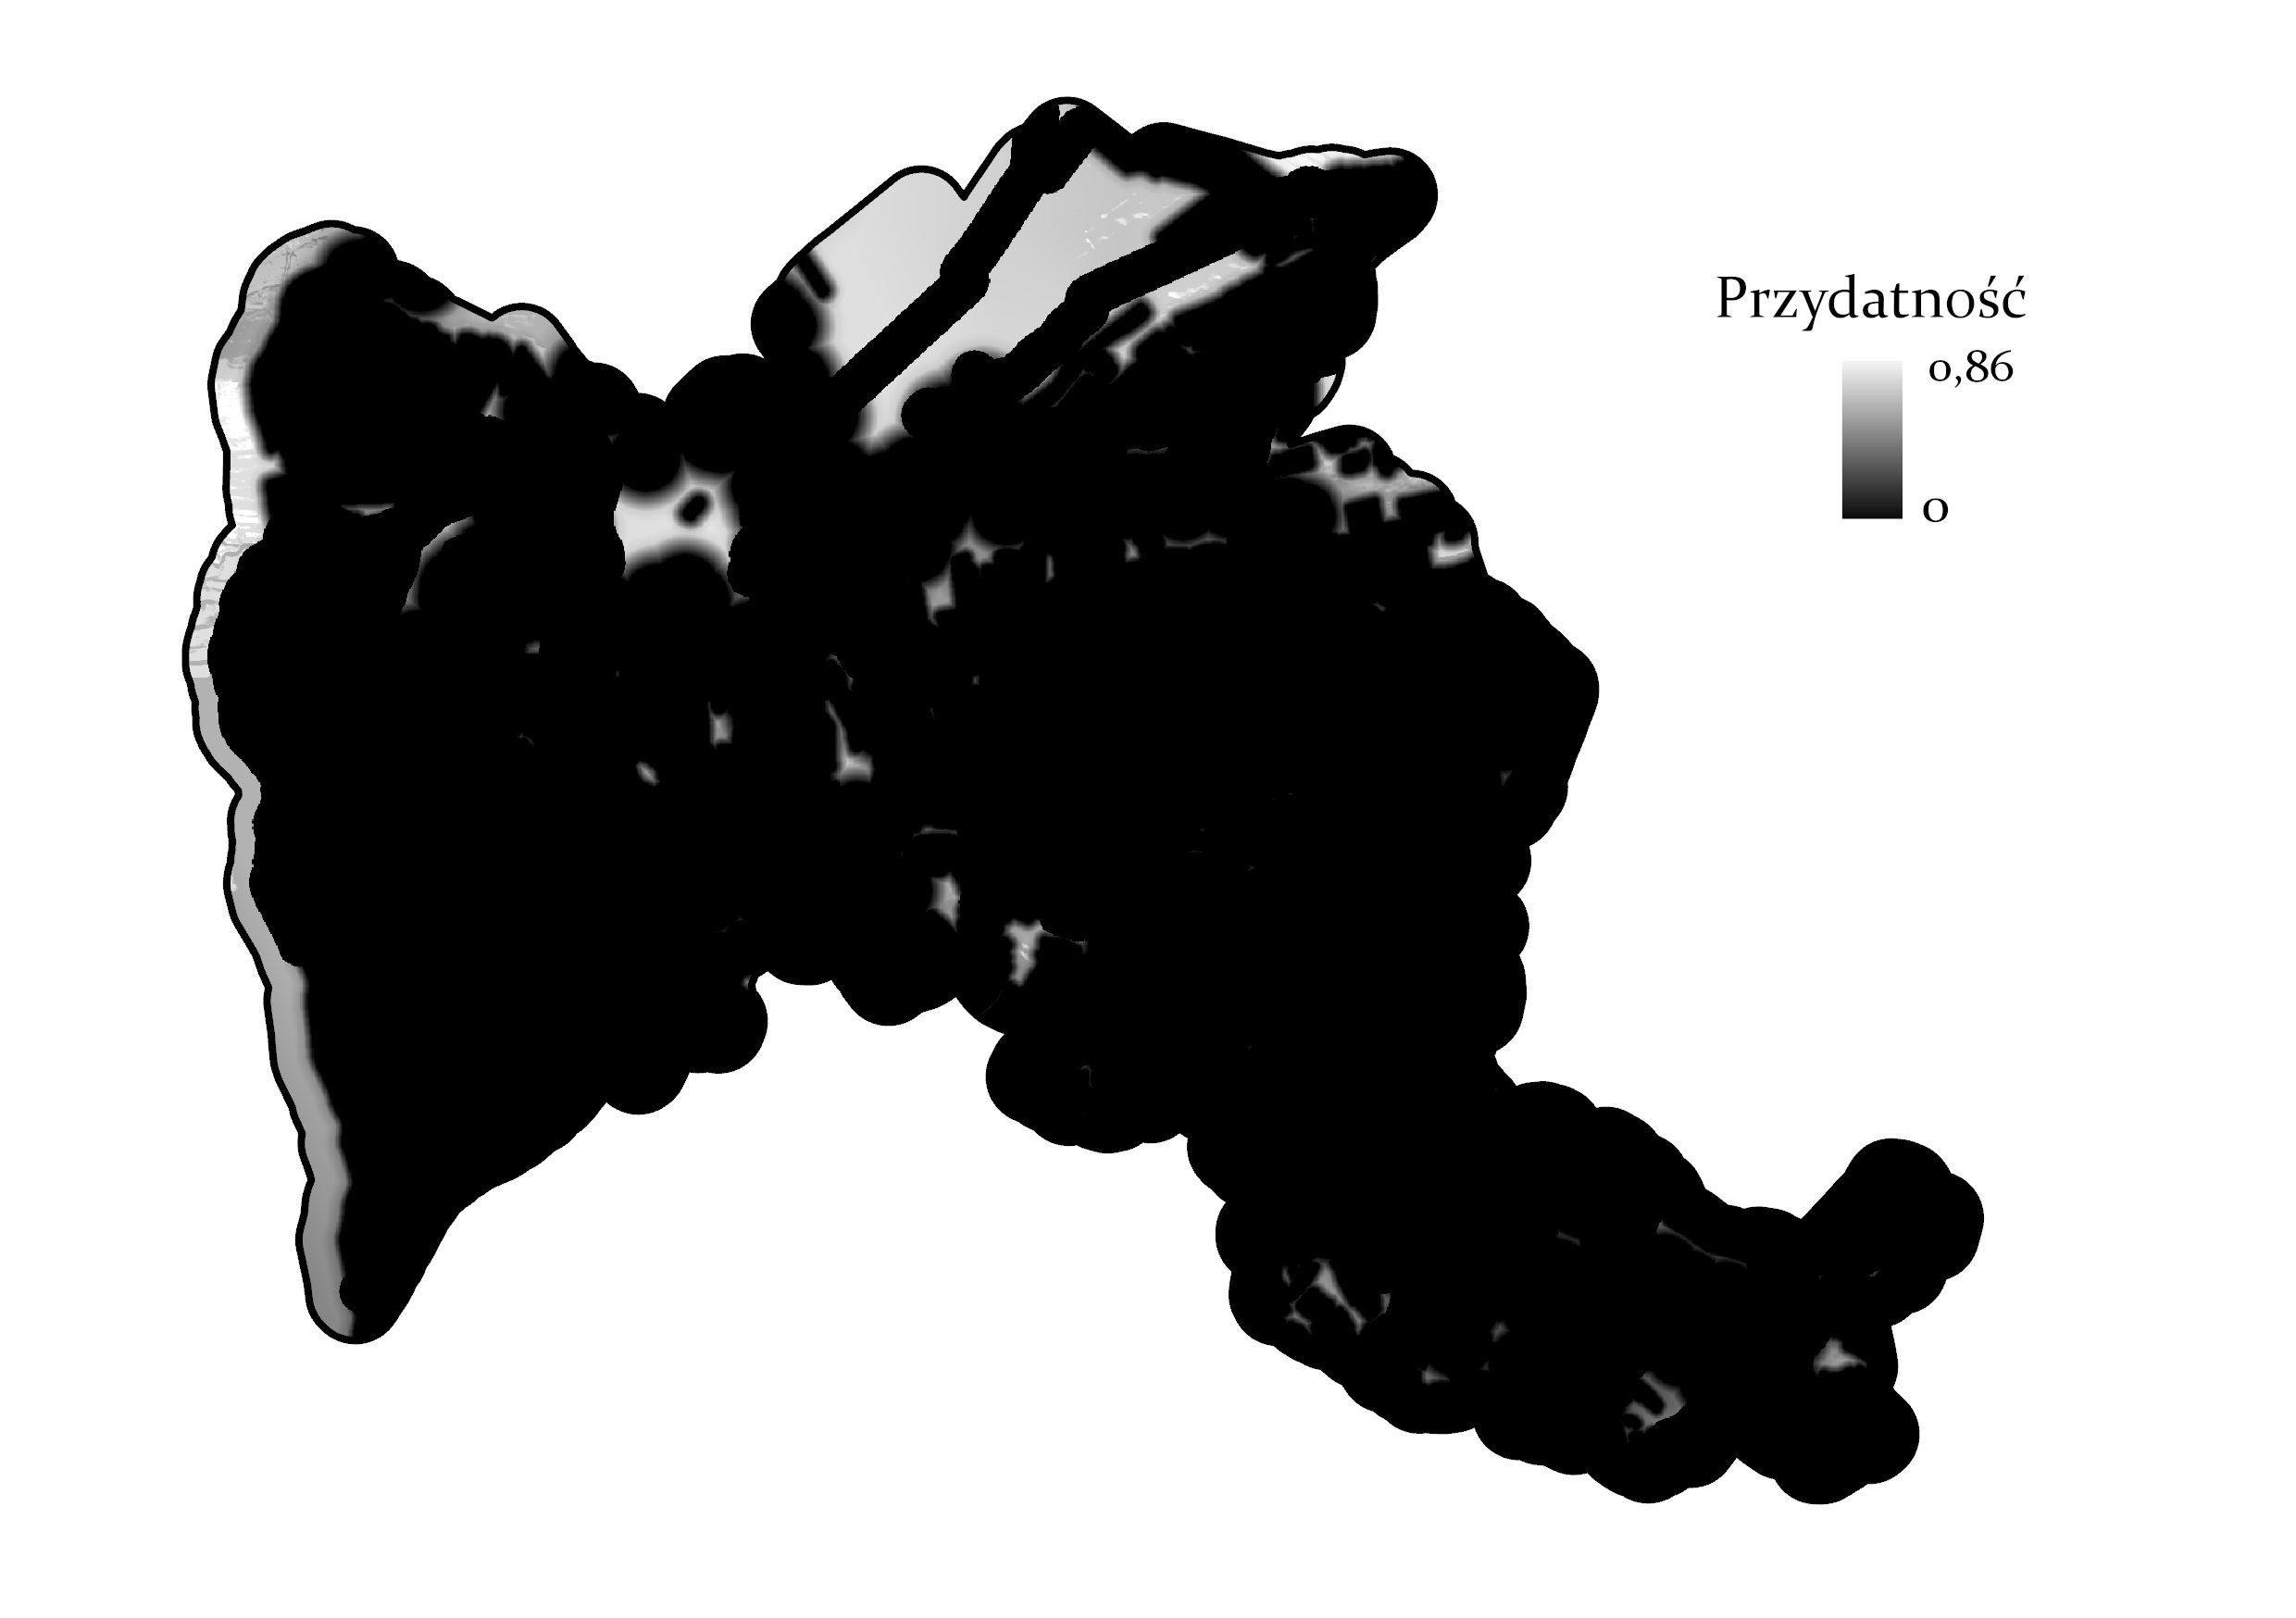
\includegraphics[width=0.75\textwidth]{img/wynik.jpg}
    \caption*{Wynik łączenia kryteriów ostrych i rozmytych}
\end{figure}

\begin{figure}[H]
    \centering
    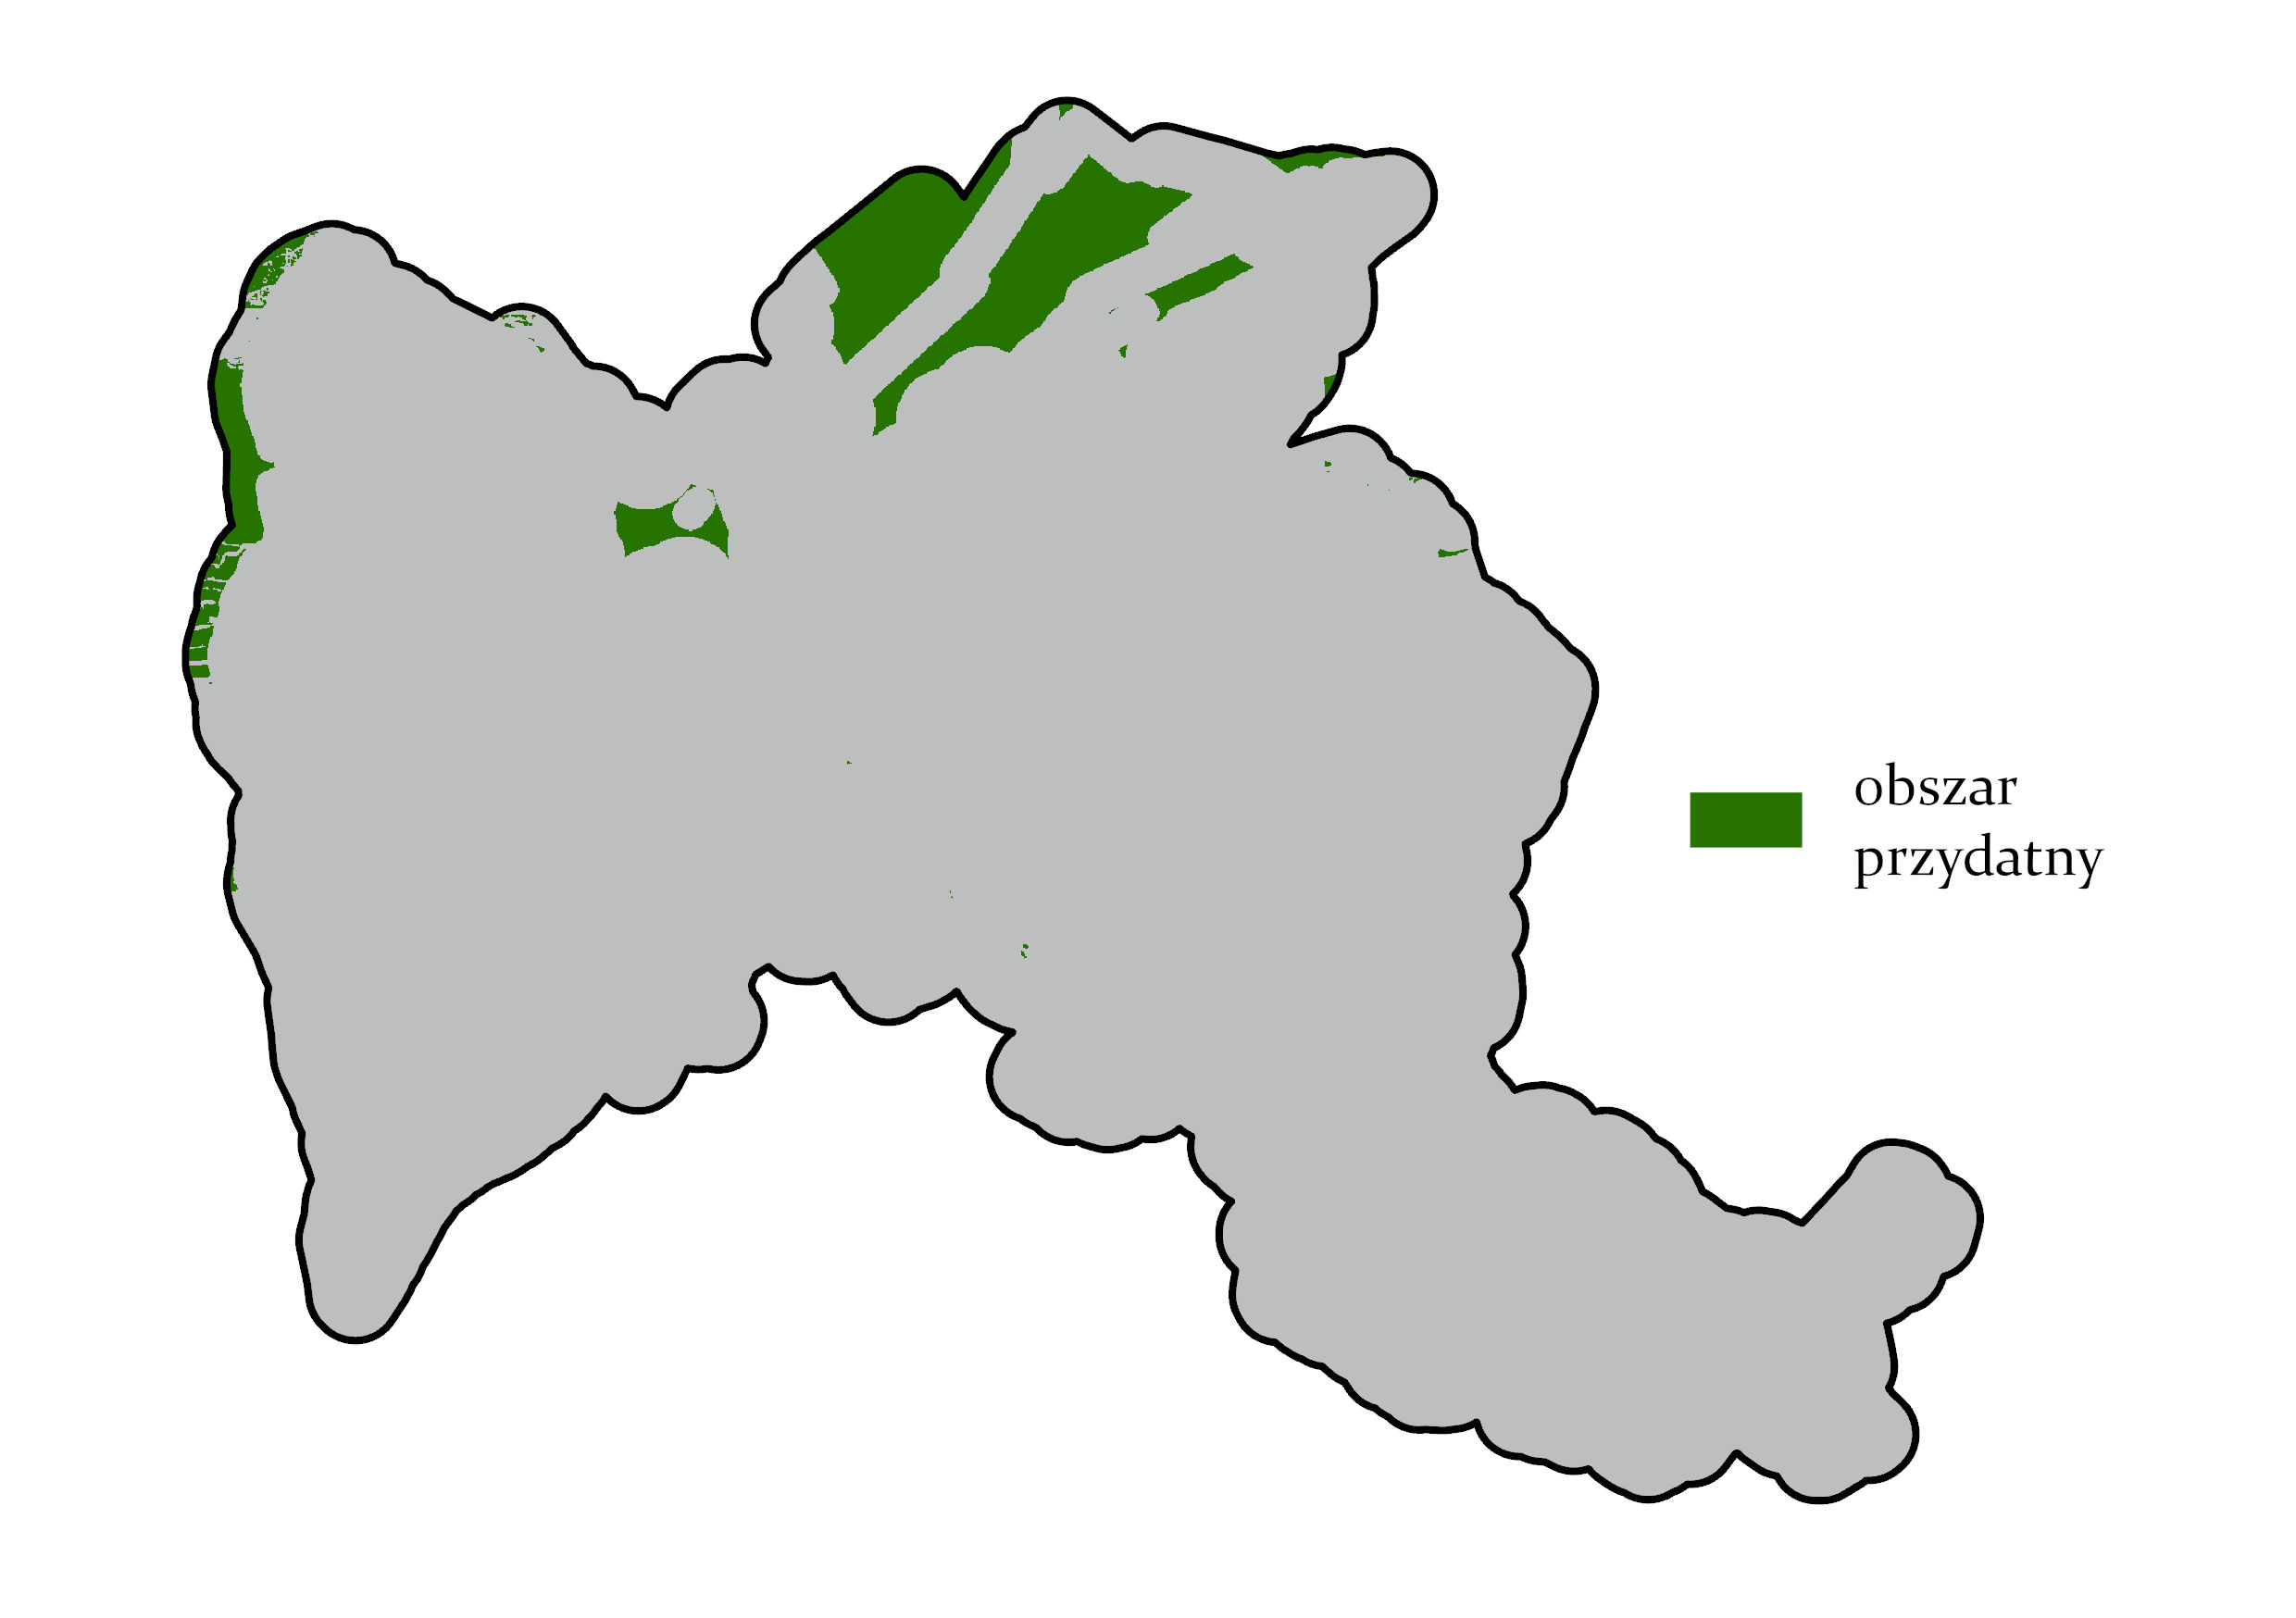
\includegraphics[width=0.75\textwidth]{img/wynik-po-reklasyfikacji.jpg}
    \caption*{Wynik łączenia kryteriów ostrych i rozmytych po reklasyfikacji}
\end{figure}


\subsection{Wybór przydatnych działek}
\subsubsection{Opis działania}
Kod najpierw zamienia uzyskany wcześniej raster na warstwę poligonową. Następnie zostają wybrane tylko te poligony, które stanowią teren przydatny.

Później warstwa z działkami zostaje przecięta powstałymi poligonami. Dzięki temu działka zostaje podzielona na części przydatne i nieprzydatne. Kolejno, aby uzyskać procentową przydatność każdej z działek, pętla przechodzi przez warstwę z działkami przeciętymi oraz pierwotną warstwę z działkami. 
Jeżeli pętla natrafi na część przydatną działki, zostaje znaleziona odpowiednia działka w warstwie pierwotnej, i pole części przydatnej działki zostaje dodane do pola pole\_przydatne.

Dzięki temu możemy obliczyć przydatność działki - stosunek powierzchni przydatnej do powierzchni całkowitej. Wybieramy jedynie te działki, których przydatność jest wyższa od wybranego progu przydatności oraz takie, które mają powierzchnię co najmniej 2ha.

\subsubsection{Kod}
\begin{lstlisting}
poligon_przydatnosci = "poligon_przydatnosci"
arcpy.conversion.RasterToPolygon(f'{geobaza}\\{wariant}_wynik_reclassified', poligon_przydatnosci, "NO_SIMPLIFY", "VALUE")

poligon_przydatnosci_layer = "poligon_przydatnosci_layer"
arcpy.management.MakeFeatureLayer(poligon_przydatnosci, poligon_przydatnosci_layer)
arcpy.management.SelectLayerByAttribute(poligon_przydatnosci_layer, "NEW_SELECTION", "gridcode = 1")
arcpy.management.CopyFeatures(poligon_przydatnosci_layer, f"{geobaza}\\{wariant}_poligon_przydatnosci")

dzialki_przeciete = "dzialki_przeciete"
arcpy.analysis.Intersect([dzialki, poligon_przydatnosci], dzialki_przeciete, "ALL")
arcpy.management.CopyFeatures(dzialki_przeciete, f"{geobaza}\\{wariant}_dzialki_przeciete_przez_poligony")

arcpy.management.AddField(dzialki_przeciete, "pole", "DOUBLE")
arcpy.management.CalculateField(dzialki_przeciete, "pole", "!shape.area@SQUAREMETERS!", "PYTHON3")

arcpy.management.AddField(dzialki, "pole", "DOUBLE")
arcpy.management.CalculateField(dzialki, "pole", "!shape.area@SQUAREMETERS!", "PYTHON3")

arcpy.management.AddField(dzialki, "pole_przydatne", "DOUBLE")
arcpy.management.CalculateField(dzialki, "pole_przydatne", 0, "PYTHON3")

with arcpy.da.UpdateCursor(dzialki_przeciete, ["ID_DZIALKI", "pole", "gridcode"]) as cursor:
    for row in cursor:
        if row[2] == 1:
            with arcpy.da.UpdateCursor(dzialki, ["ID_DZIALKI", "pole", "pole_przydatne"]) as cursor2:
                for row2 in cursor2:
                    if row[0] == row2[0]:
                        row2[2] += row[1]
                        cursor2.updateRow(row2)

arcpy.management.AddField(dzialki, "przydatnosc", "DOUBLE")
arcpy.management.CalculateField(dzialki, "przydatnosc", "(!pole_przydatne! / !pole!) * 100", "PYTHON3")

dzialki_layer = "dzialki_layer"
arcpy.management.MakeFeatureLayer(dzialki, dzialki_layer)
arcpy.management.SelectLayerByAttribute(dzialki_layer, "NEW_SELECTION", f"przydatnosc > {prog_przydatnosci} AND shape_area > 20000 ")
arcpy.management.CopyFeatures(dzialki_layer, f"{geobaza}\\{wariant}_dzialki_przydatne_powyzej_{prog_przydatnosci}")
\end{lstlisting}

\begin{figure}[H]
    \centering
    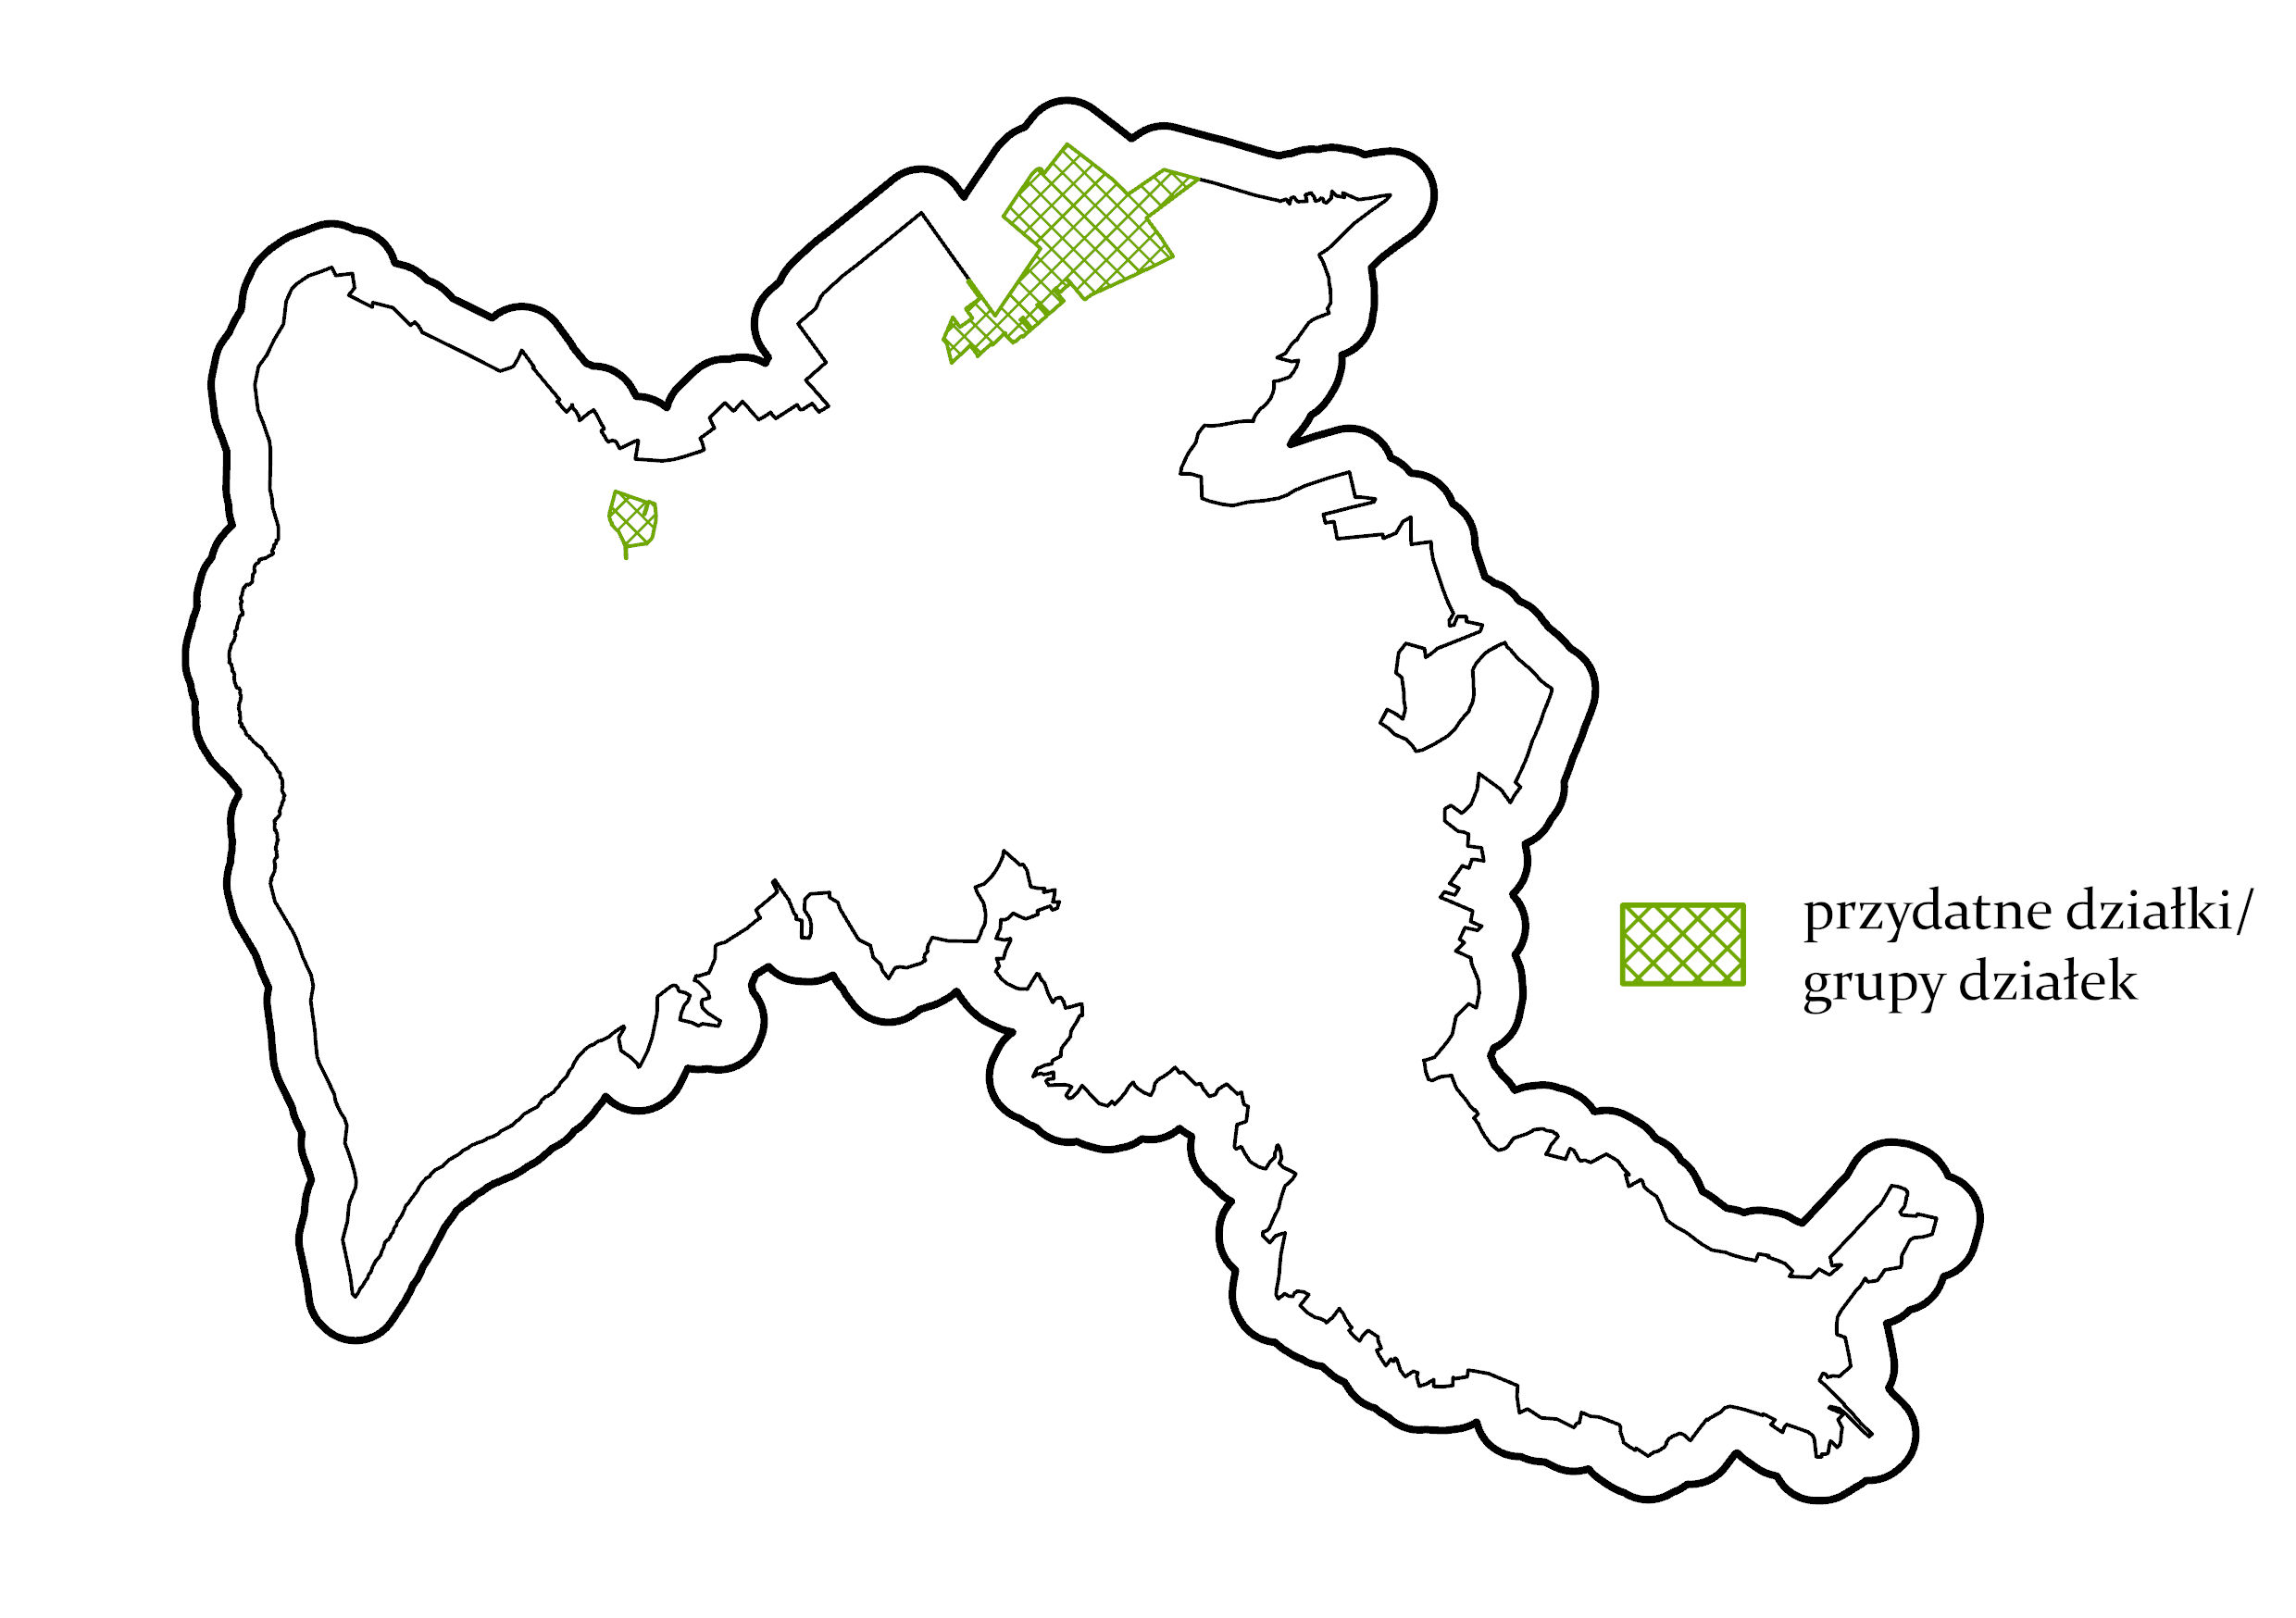
\includegraphics[width=0.75\textwidth]{img/przydatne-dzialki.jpg}
    \caption*{Mapa przedstawiająca przydatne działki}
\end{figure}

\begin{figure}[H]
    \centering
    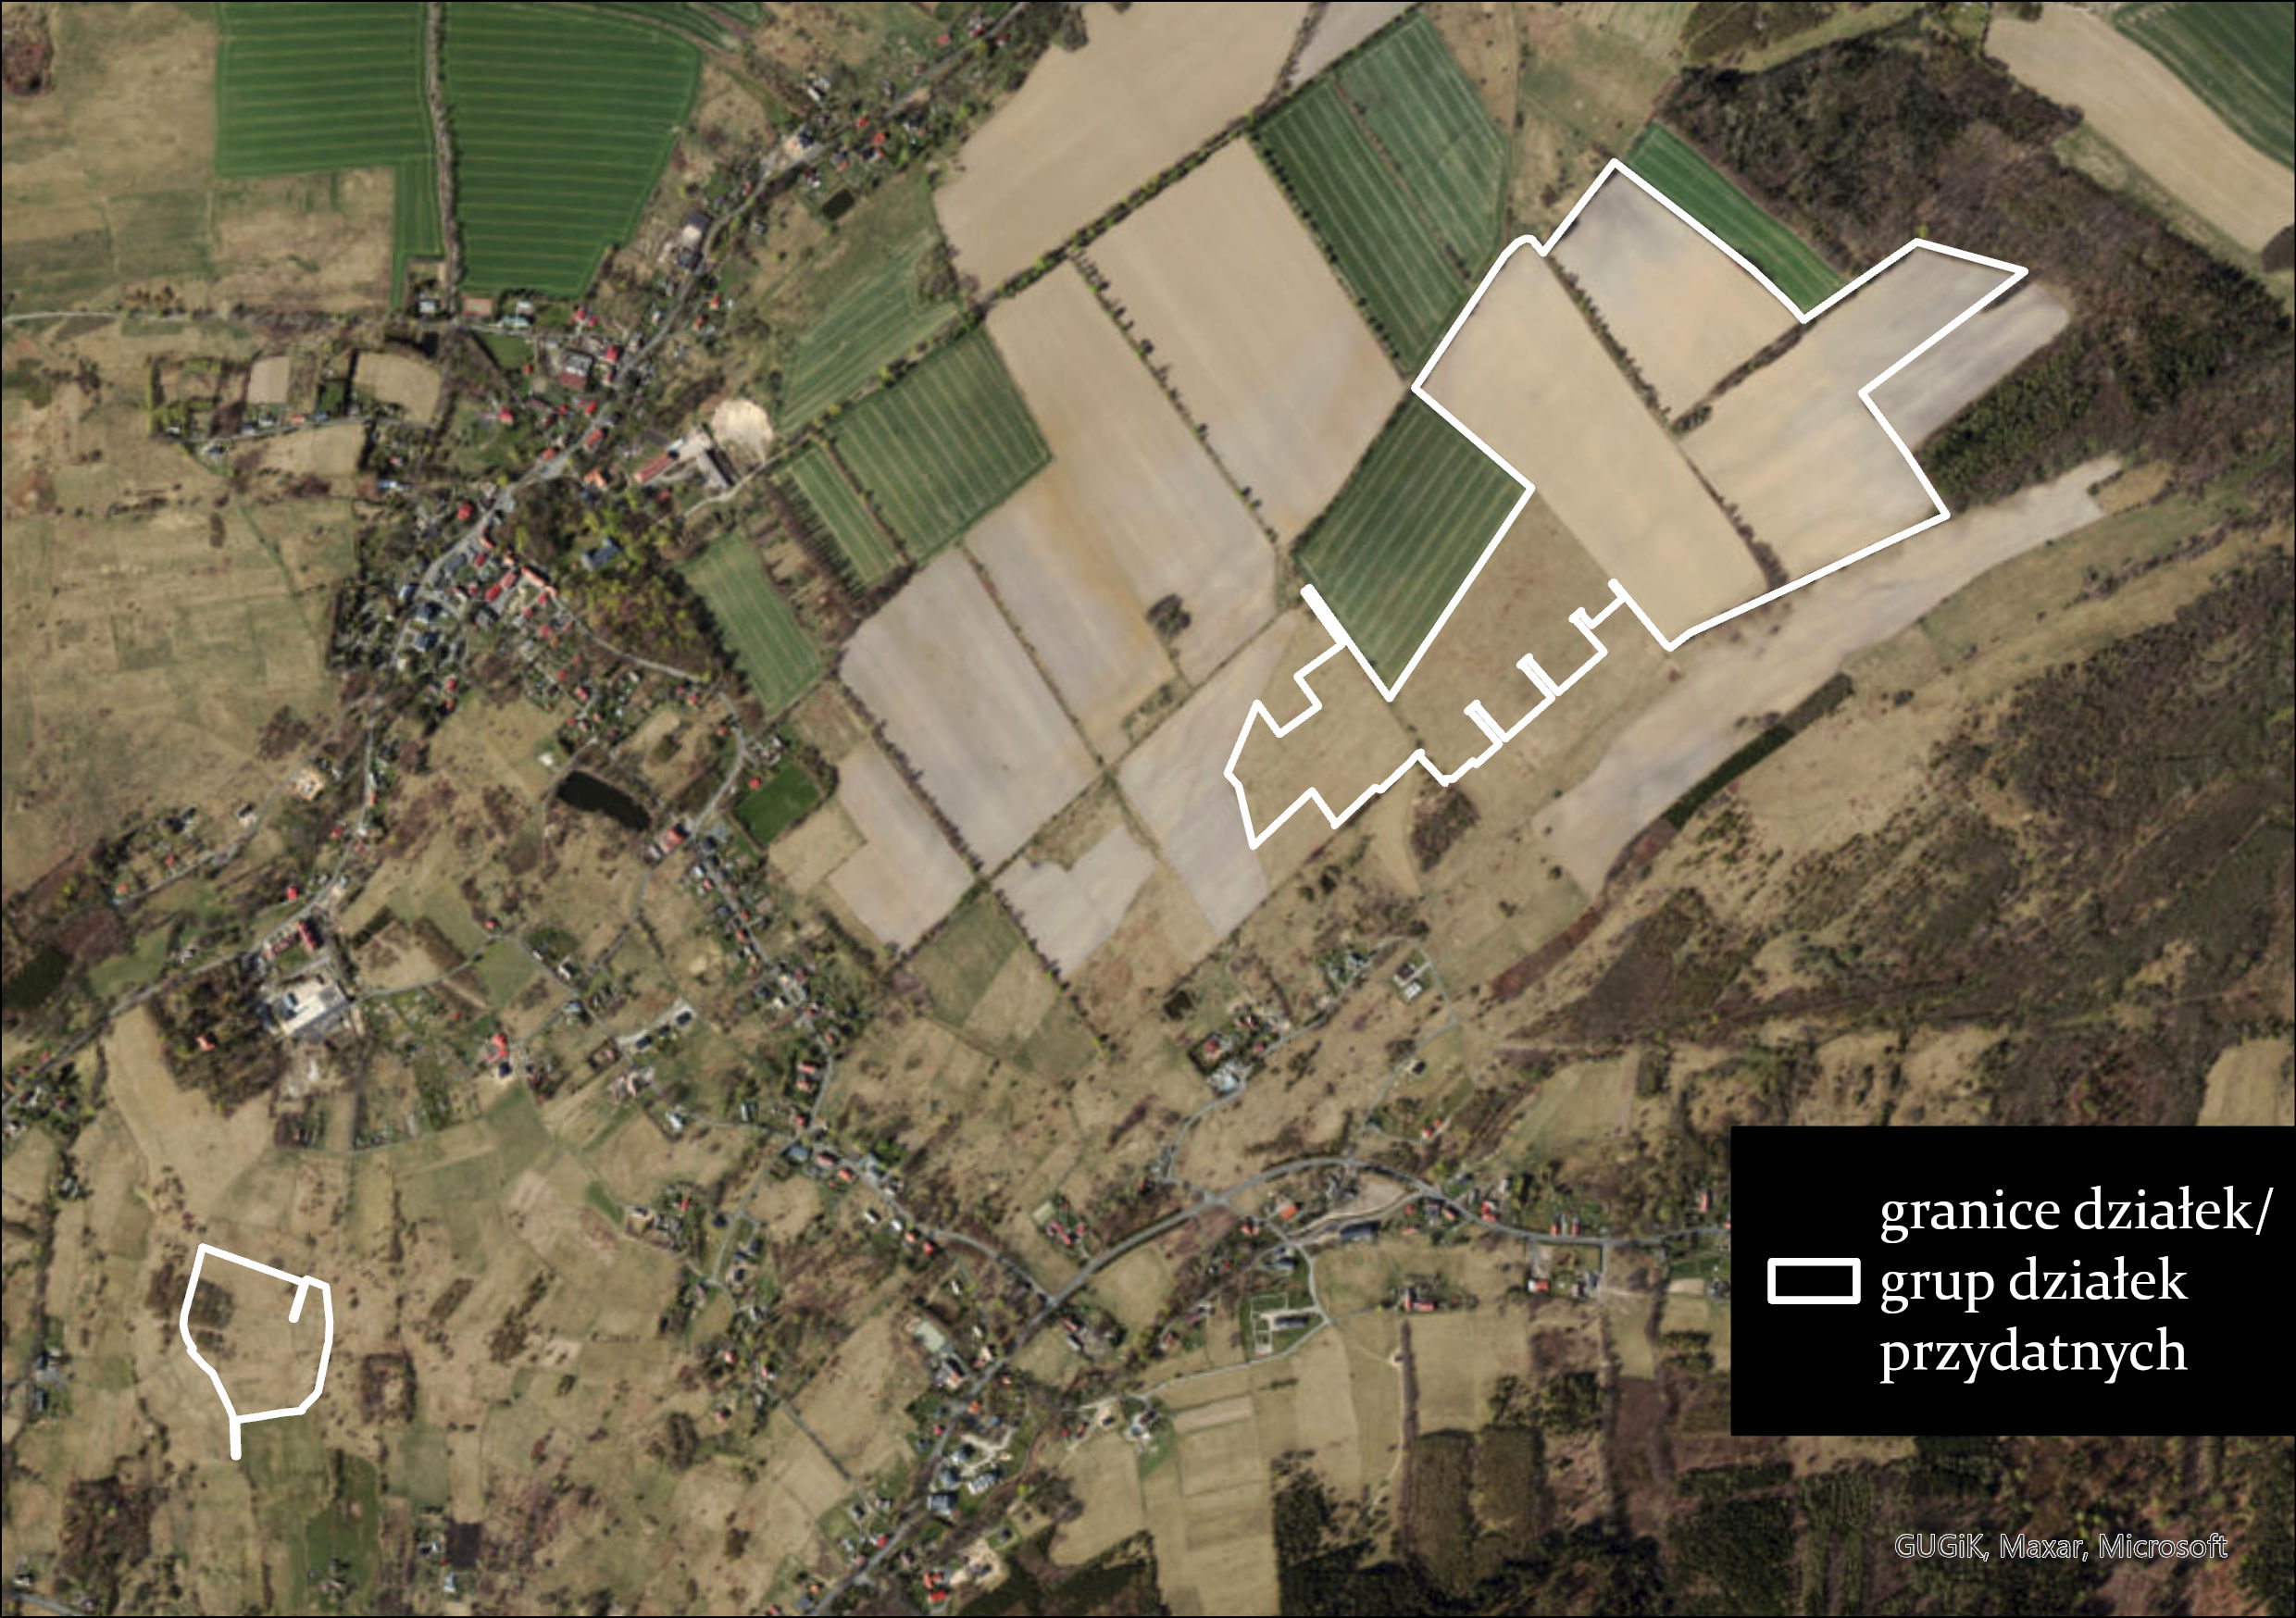
\includegraphics[width=0.75\textwidth]{img/dzialki-przydatne-ortofoto.jpg}
    \caption*{Mapa przedstawiająca przydatne działki na ortofotomapie}
\end{figure}

\subsection{Koszt przyłącza do sieci SN}
\subsubsection{Opis działania}
Przed rozpoczęciem analiz należało stworzyć tzw. mapę kosztów względnych(jednostkowych), która przedstawia faktyczną lub umowną wartość kosztu zbudowania
przyłącza przez dany obszar. Dla mapy kosztów względnych w postaci rastrowej, będzie to względny koszt budowy przyłącza na obszarze o powierzchni odpowiadającej rozmiarowi
piksela. W ćwiczeniu przyjęto, że koszt = 1 jest odniesiony do obszarów rolniczych (najmniejszy koszt prac ziemnych / budowlanych dla 1 piksela). Koszty względne dla innych obszarów są obliczane jako wielokrotność kosztów dla terenów rolniczych. Przypisane koszty dla wszystkich kategorii użytkowania terenu dla doprowadzenia do
farmy przyłącza przedstawia tabela.

Następnie, dla każdego obiektu połączonej warstwy zawierającej pokrycie terenu gminy dodano odpowiedni koszt, na podstawie pola x\_kod, mówiącego o typie terenu, jaki stanowi. Warstwę nastepnie zamieniamy na raster, wykorzystując do tego nowo dodane pole z kosztem. Tworzymy mapę kosztów skumulowanych (cost map) oraz mapę kierunków (backlink raster) z użyciem narzędzia Cost Distance. Wykorzystując utworzone mapy, tworzymy ścieżkę przyłącza o najmniejszym koszcie (cost path). Rastrowa ścieżka zostaje przekonwertowana na warstwę wektorową.

\begin{figure}[H]
    \centering
    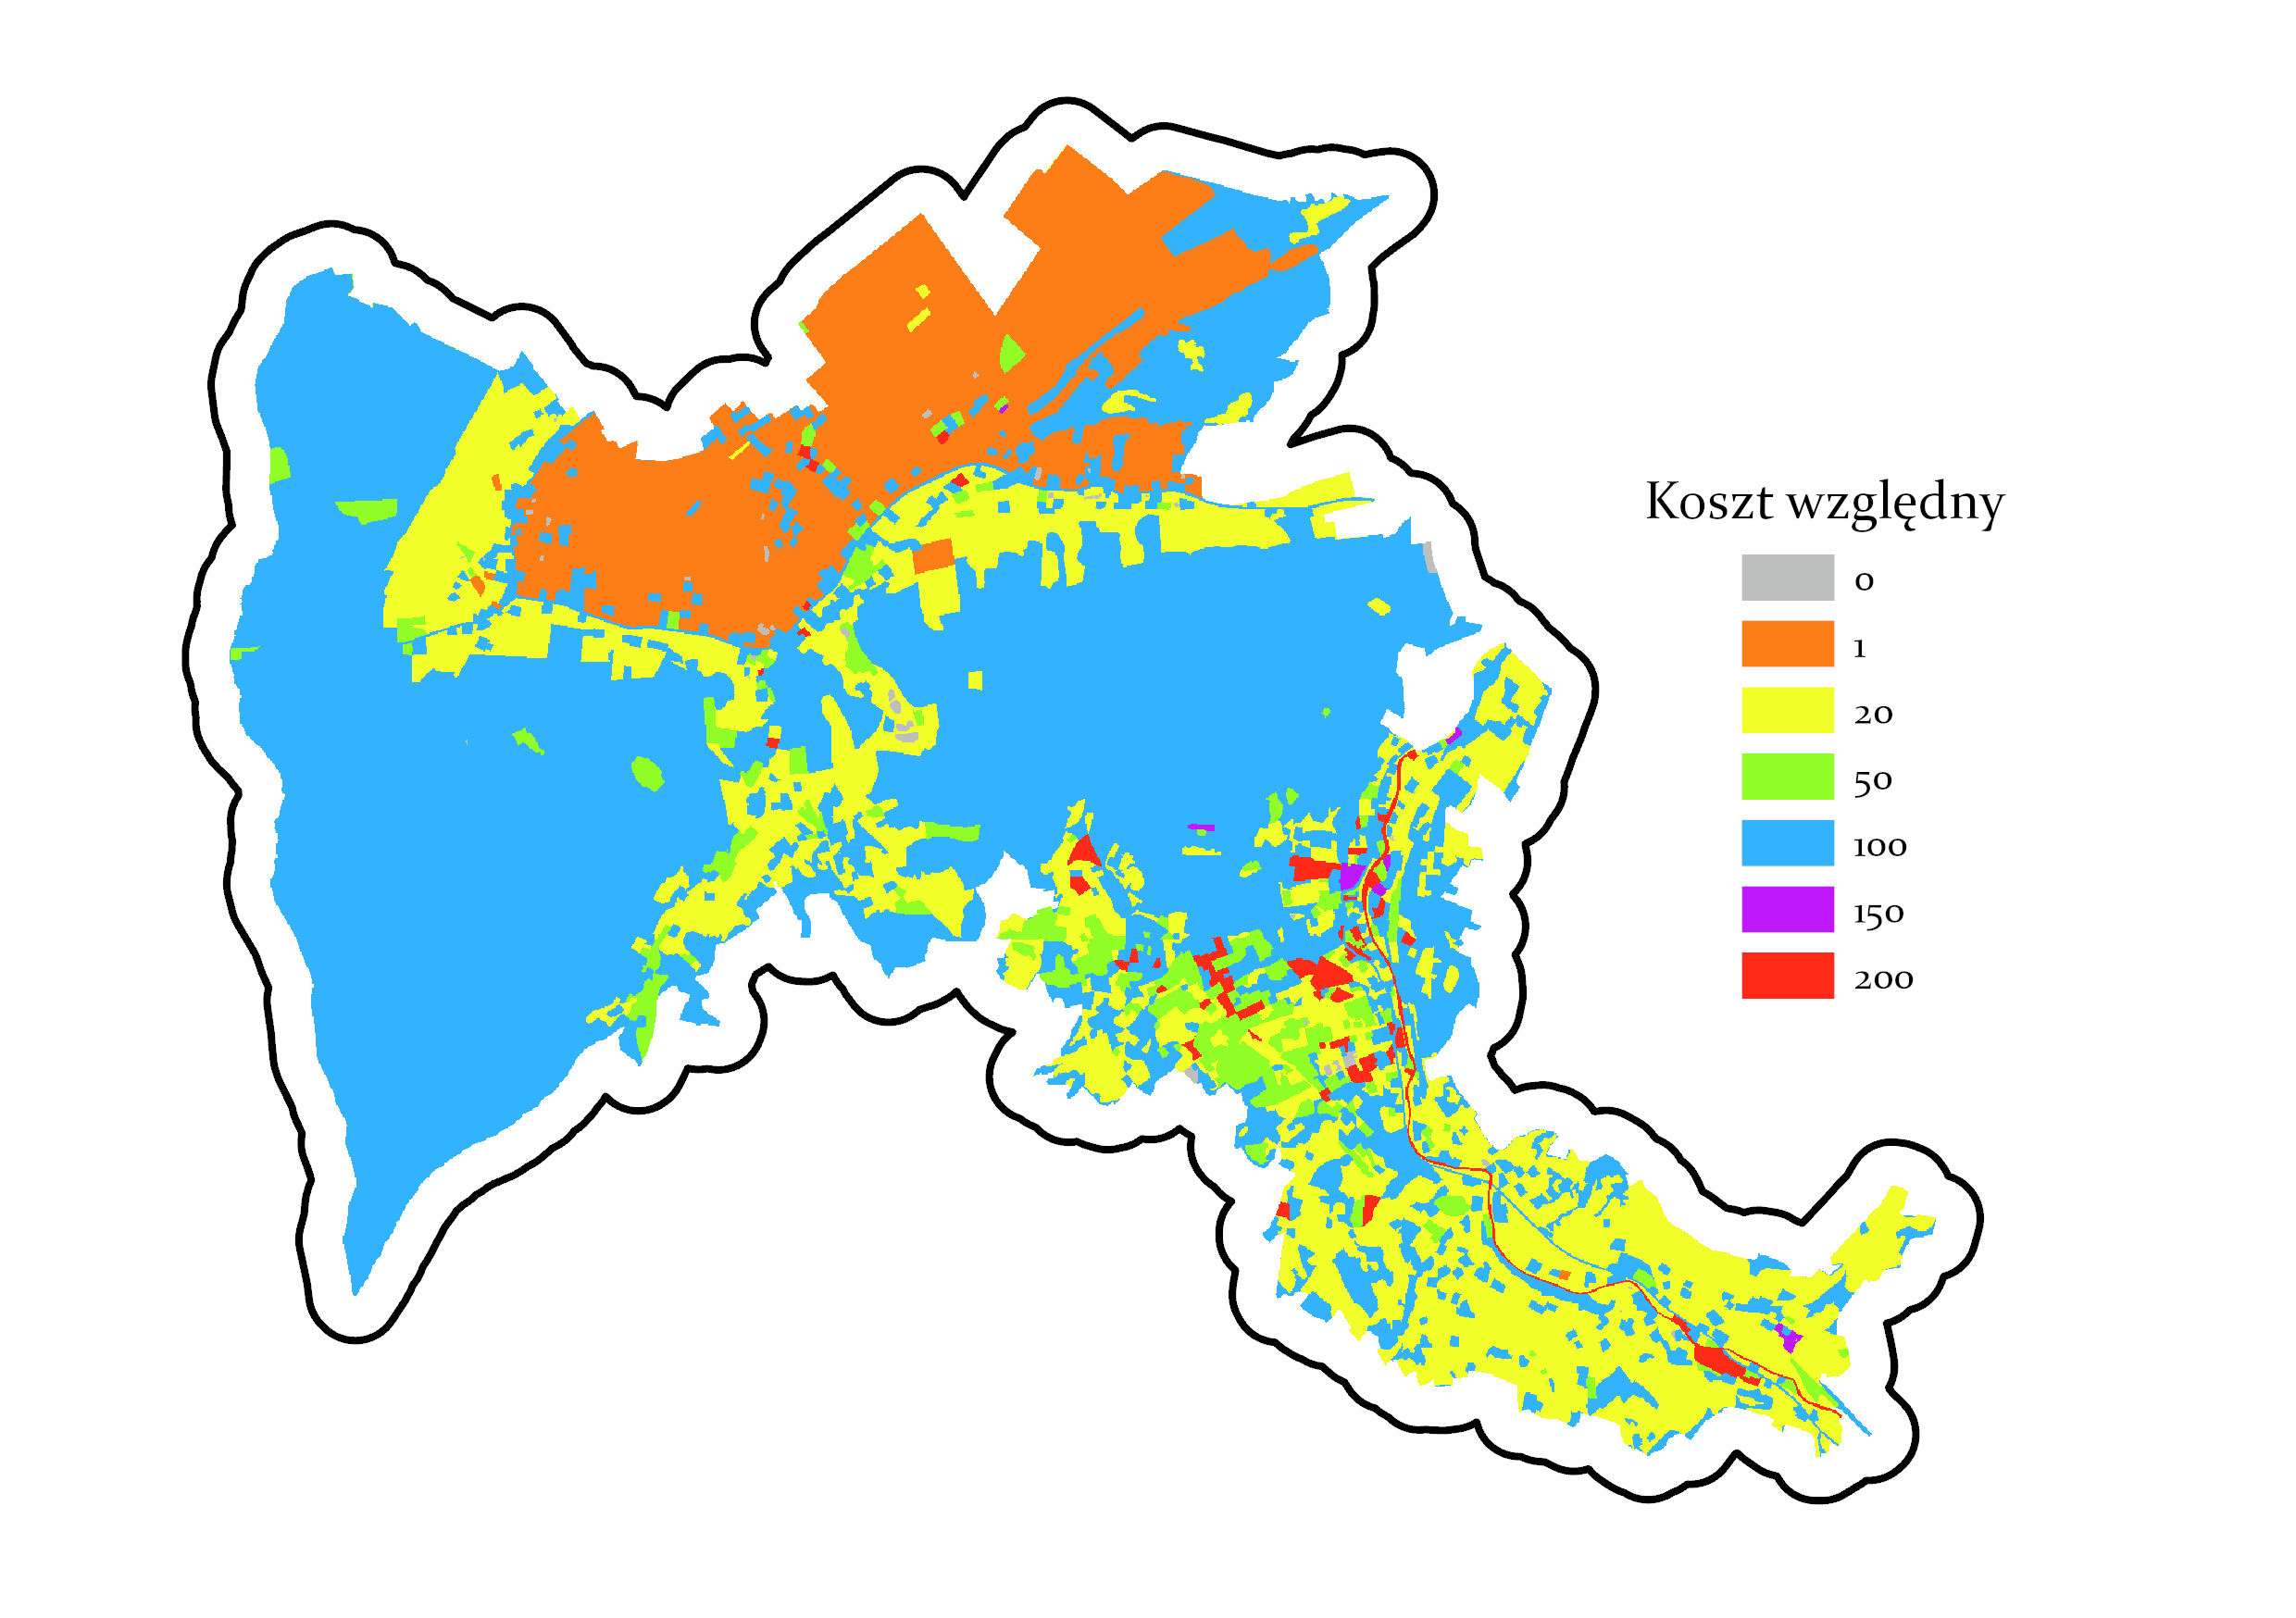
\includegraphics[width=0.75\textwidth]{img/cost-raster.jpg}
    \caption*{Mapa kosztów względnych}
\end{figure}

% \begin{table}[ht]
%     \centering % Wyśrodkowanie tabeli
%     \renewcommand{\arraystretch}{1.2} % Zwiększenie odstępów między wierszami
%     \begin{tabular}{|p{2cm}|p{4.5cm}|p{2cm}|p{3cm}|p{2cm}|}
%     \hline
%     \textbf{Kod klasy obiektów BDOT} & \textbf{Nazwa klasy obiektów BDOT} & \textbf{X\_kod} & \textbf{Typ obiektu} & \textbf{Koszt względny} \\
%     \hline
%     PTWP & woda powierzchniowa & PTWP01 & woda morska & 0 $\rightarrow$ NoData \\ \cline{3-5}
%     & & PTWP02 & woda płynąca & 200 \\ \cline{3-5}
%     & & PTWP03 & woda stojąca & 0 $\rightarrow$ NoData \\ 
%     \hline
%     PTZB & zabudowa & PTZB02 & jednorodzinna & 100 \\ \cline{3-5}
%     & & PTZB01 & wielorodzinna & 200 \\ \cline{3-5}
%     & & PTZB05 & pozostała \newline zabudowa & 50 \\ \cline{3-5}
%     & & PTZB04 & handlowo-usługowa & 200 \\ \cline{3-5}
%     & & PTZB03 & przemysłowo-składowa & 200 \\ 
%     \hline
%     PTLZ & teren leśny i zadrzewiony & PTLZ01 & las & 100 \\ \cline{3-5}
%     & & PTLZ02 & zagajnik & 50 \\ \cline{3-5}
%     & & PTLZ03 & zadrzewienie & 50 \\ 
%     \hline
%     PTRK & roślinność krzewiasta & PTRK01 & kępy krzewów & 20 \\ \cline{3-5}
%     & & PTRK02 & krzewy & 15 \\ 
%     \hline
%     PTUT & uprawa trwała & PTUT03 & sad & 100 \\ \cline{3-5}
%     & & PTUT02 & plantacja & 90 \\ \cline{3-5}
%     & & PTUT04, PTUT05 & inne & 20 \\ \cline{3-5}
%     & & PTUT01 & ogród działkowy & 0 $\rightarrow$ NoData \\ 
%     \hline
%     PTTR & roślinność trawiasta i uprawa rolna & PTTR02 & grunt orny & 1 \\ \cline{3-5}
%     & & PTTR01 & roślinność \newline trawiasta & 20 \\ 
%     \hline
%     PTKM & teren pod drogami kołowymi, szynowymi i lotniskowymi & PTKM02 & torowisko & 200 \\ \cline{3-5}
%     & & PTKM01 & droga kołowa & 200 \\ \cline{3-5}
%     & & PTKM03 & teren pod drogą \newline kołową \newline i torowiskiem & 200 \\ \cline{3-5}
%     & & PTKM04 & teren pod drogą \newline lotniskową & 0 $\rightarrow$ NoData \\ 
%     \hline
%     PTGN & grunt nieużytkowany & PTGN01, PTGN02, PTGN03, PTGN04 & - & 1 \\ 
%     \hline
%     PTPL & plac & PTPL01 & - & 50 \\ 
%     \hline
%     PTSO & składowisko odpadów & PTSO01, PTSO02 & - & 0 $\rightarrow$ NoData \\ 
%     \hline
%     PTWZ & wyrobisko i zwałowisko & PTWZ01, PTWZ02 & - & 0 $\rightarrow$ NoData \\ 
%     \hline
%     PTNZ & pozostały teren niezabudowany & PTNZ01, PTNZ02 & - & 150 \\ 
%     \hline
%     \end{tabular}
%     \caption{Tabela kosztów względnych dla różnych typów obiektów BDOT.}
%     \label{tab:bdot_costs}
% \end{table}

\subsubsection{Kod}
\begin{lstlisting}
pt_merged_layer = "pt_merged_layer"
arcpy.management.MakeFeatureLayer(pt_merged, pt_merged_layer)
arcpy.management.AddField(pt_merged_layer, "cost", "FLOAT")
arcpy.management.CalculateField(
    in_table=pt_merged_layer,
    field="cost",
    expression="costs.get(!x_kod!, 0)",
    expression_type="PYTHON3",
    code_block="""costs = {
    "PTWP01": 0, 
    "PTWP02": 200,
    "PTWP03": 0,
    "PTZB02": 100,
    "PTZB01": 200,
    "PTZB05": 50,
    "PTZB04": 200,
    "PTZB03": 200,
    "PTLZ01": 100,
    "PTLZ02": 50,
    "PTLZ03": 50,
    "PTRK01": 15,
    "PTRK02": 15,
    "PTUT03": 100,
    "PTUT02": 90,
    "PTUT04": 20,
    "PTUT05": 20,
    "PTUT01": 0,
    "PTTR02": 1,
    "PTTR01": 20,
    "PTKM02": 200,
    "PTKM01": 100,
    "PTKM03": 200,
    "PTKM04": 0,
    "PTGN01": 1,
    "PTGN02": 1,
    "PTGN03": 1,
    "PTGN04": 1,
    "PTPL01": 50,
    "PTSO01": 0,
    "PTSO02": 0,
    "PTWZ01": 0,
    "PTWZ02": 0,
    "PTNZ01": 150,
    "PTNZ02": 150
    }"""
)

out_cost = arcpy.conversion.PolygonToRaster(
    in_features=pt_merged_layer,
    value_field="cost",
    out_rasterdataset=f"{geobaza}\\{wariant}_cost_raster",
    cell_assignment="CELL_CENTER",
    cellsize=5
)

out_distance = arcpy.sa.CostDistance(
    in_source_data=f"{geobaza}\\{wariant}_dzialki_przydatne_powyzej_{prog_przydatnosci}",
    in_cost_raster=f"{geobaza}\\{wariant}_cost_raster",
    maximum_distance=None,
    out_backlink_raster=f"{geobaza}\\{wariant}_cost_backlink",
    source_cost_multiplier=None,
    source_start_cost=None,
    source_resistance_rate=None,
    source_capacity=None,
    source_direction=""
)
out_distance.save(f"{geobaza}\\{wariant}_cost_distance")

out_path = arcpy.sa.CostPath(
    in_destination_data=linie_elektroenergetyczne,
    in_cost_distance_raster=f"{geobaza}\\{wariant}_cost_distance",
    in_cost_backlink_raster=f"{geobaza}\\{wariant}_cost_backlink",
    path_type="BEST_SINGLE",
    force_flow_direction_convention="INPUT_RANGE"
)
out_path.save(f"{geobaza}\\{wariant}_cost_path")

path_vector = arcpy.conversion.RasterToPolyline(in_raster=out_path, out_polyline_features=f"{geobaza}\\{wariant}_cost_path_vector")
\end{lstlisting}

\subsubsection{Wynik}

\begin{figure}[H]
    \centering
    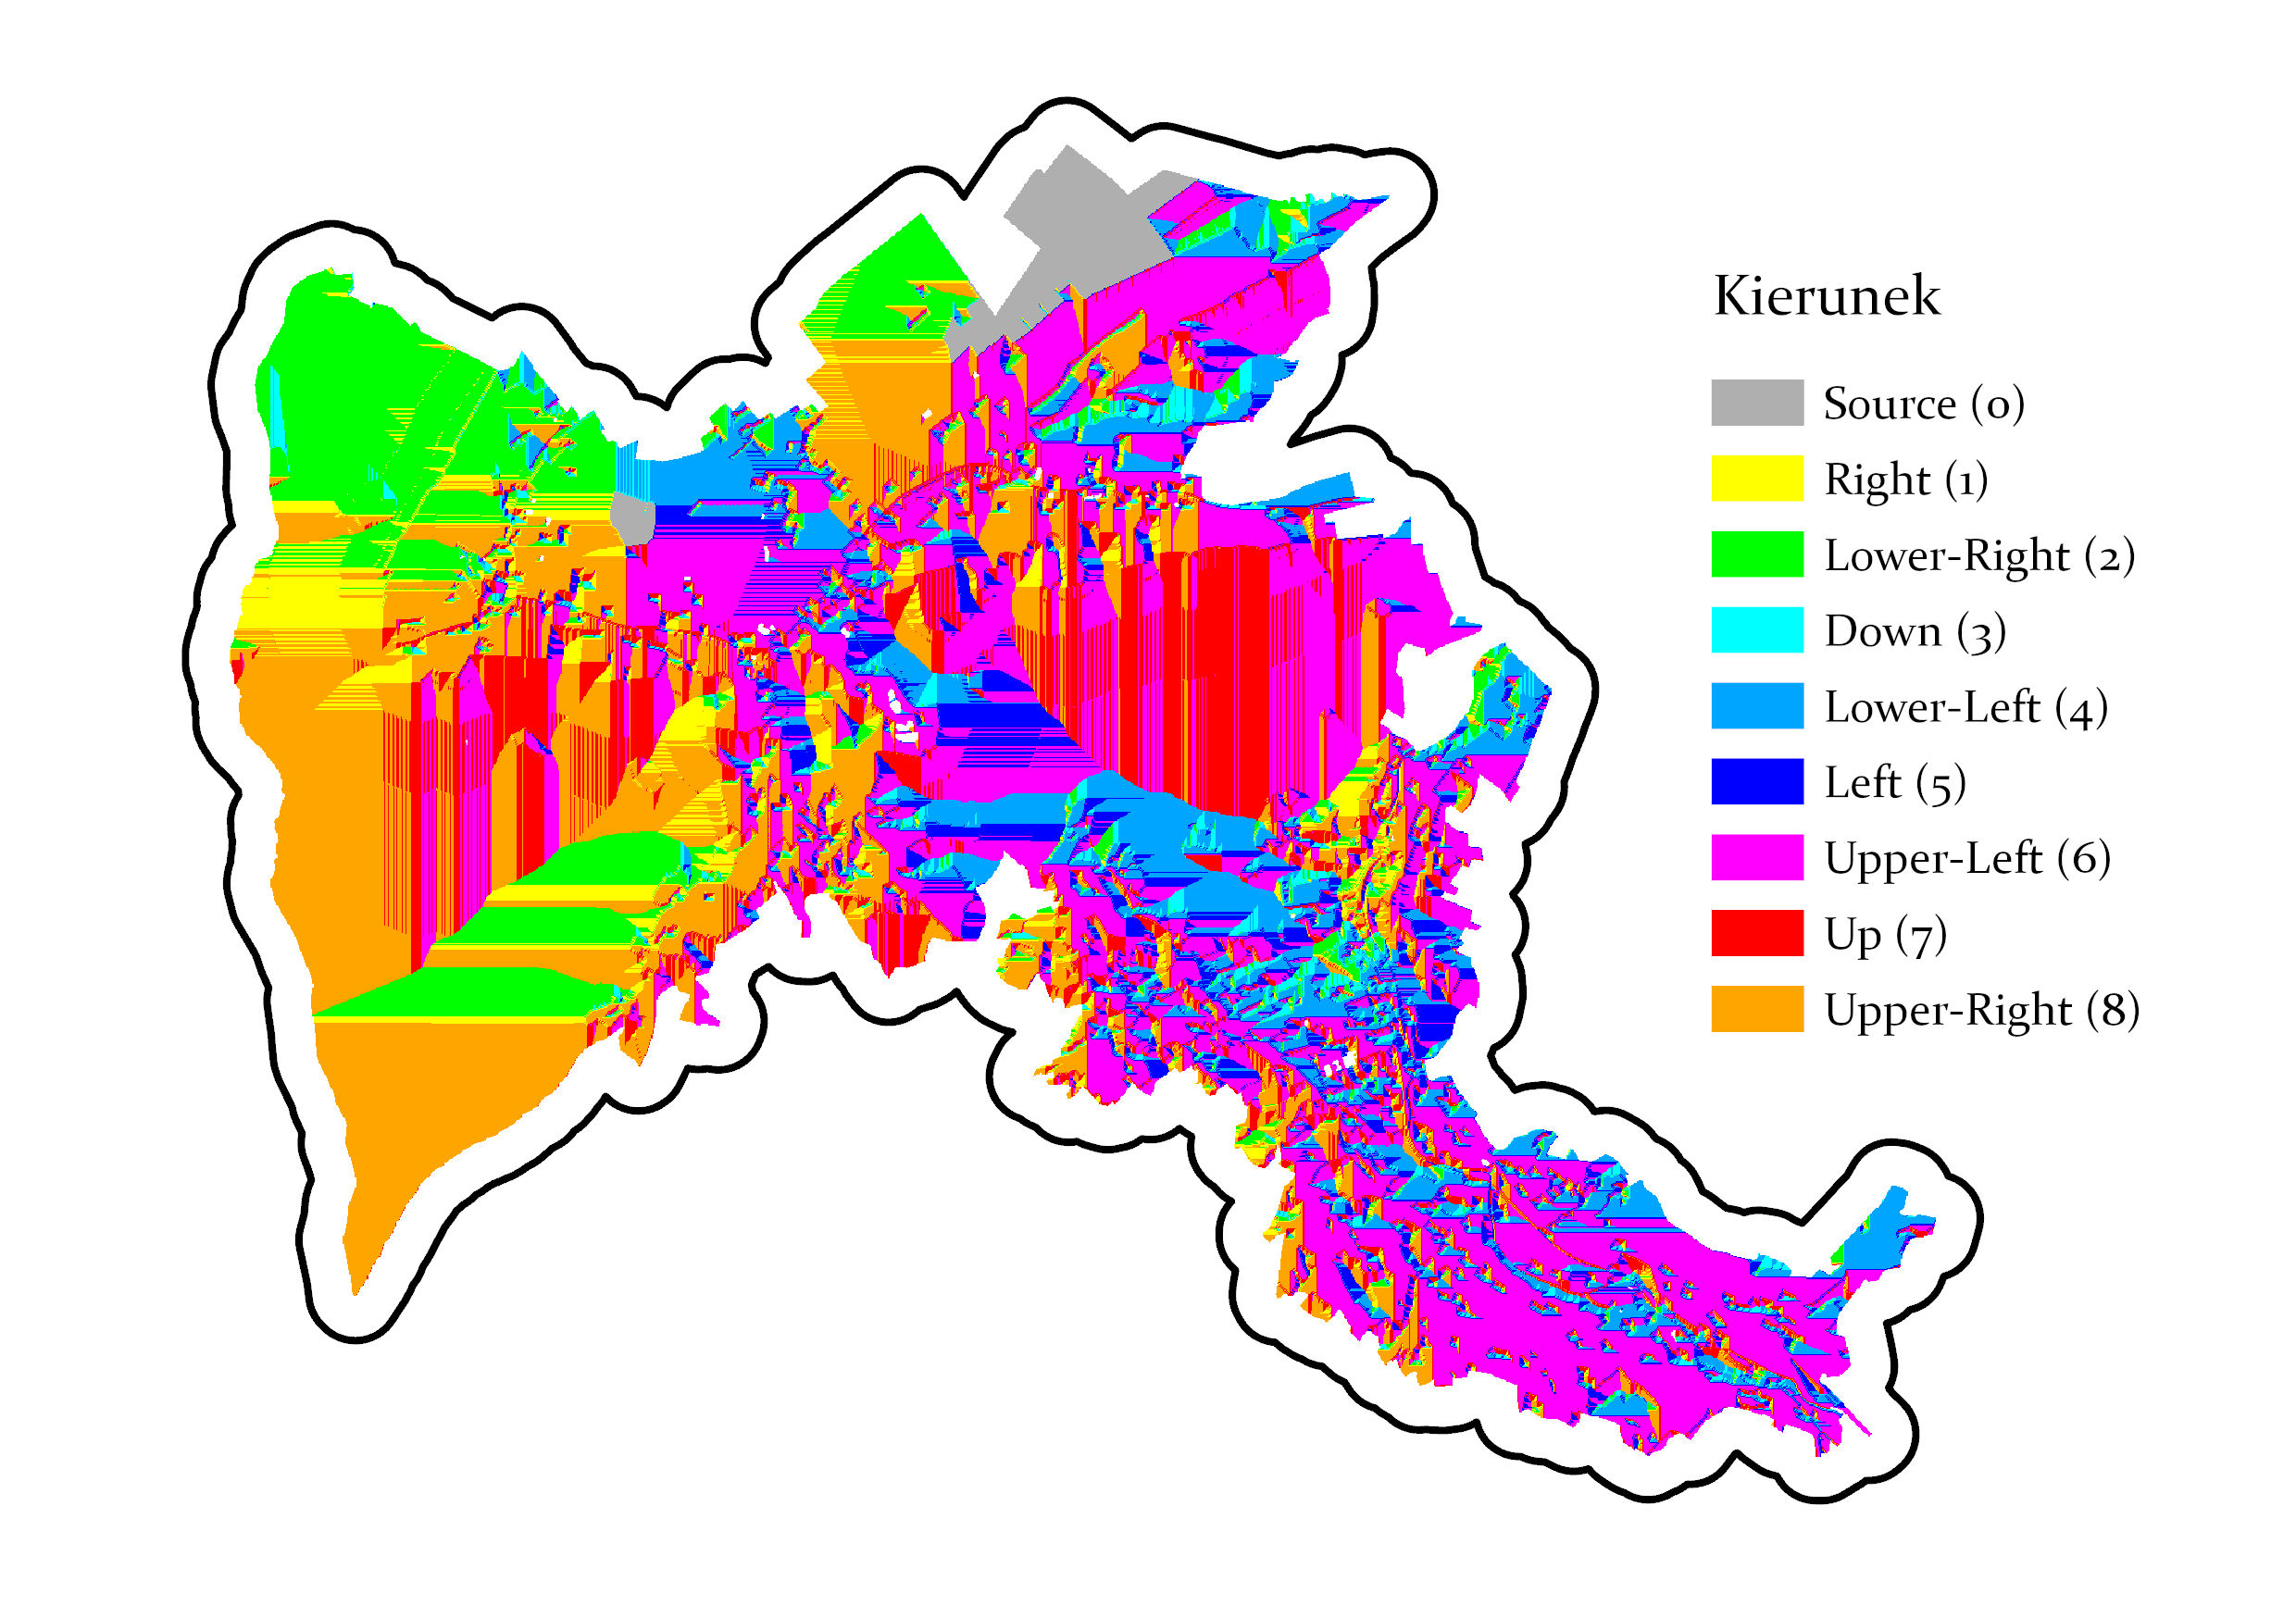
\includegraphics[width=0.75\textwidth]{img/cost-backlink.jpg}
    \caption*{Mapa kierunków (backlink)}
\end{figure}

\begin{figure}[H]
    \centering
    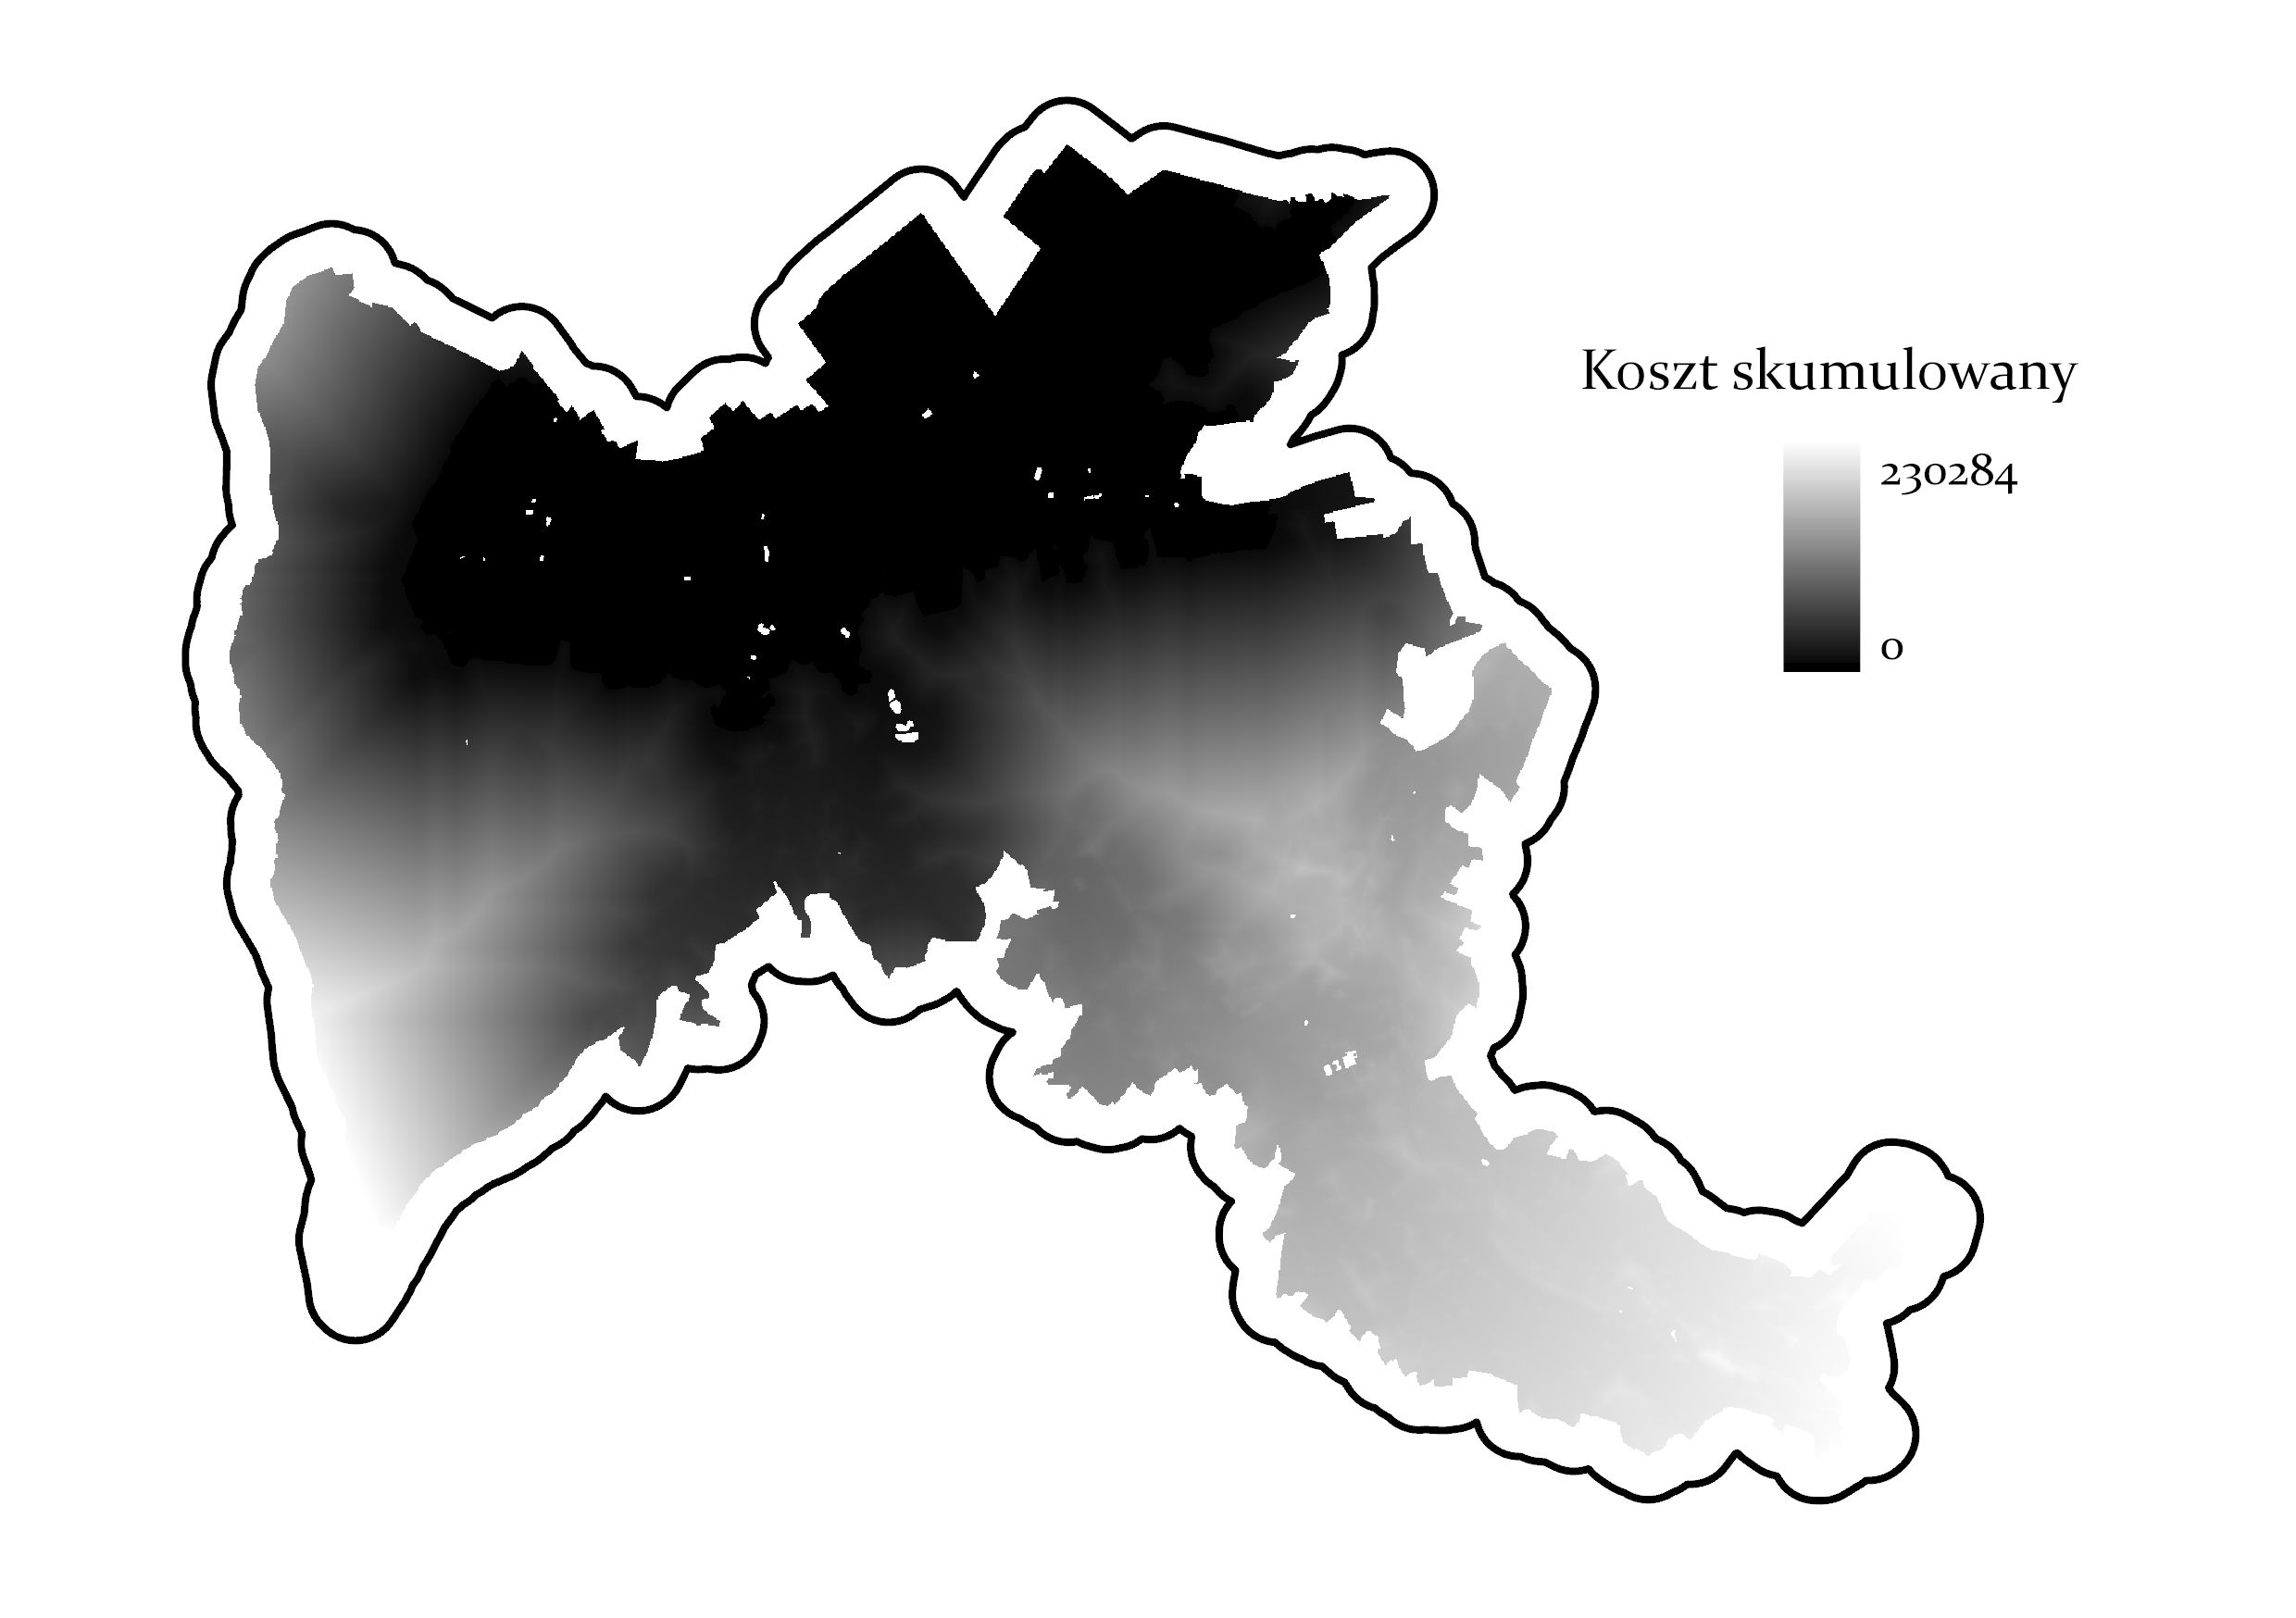
\includegraphics[width=0.75\textwidth]{img/cost-distance.jpg}
    \caption*{Mapa kosztów skumulowanych}
\end{figure}

\begin{figure}[H]
    \centering
    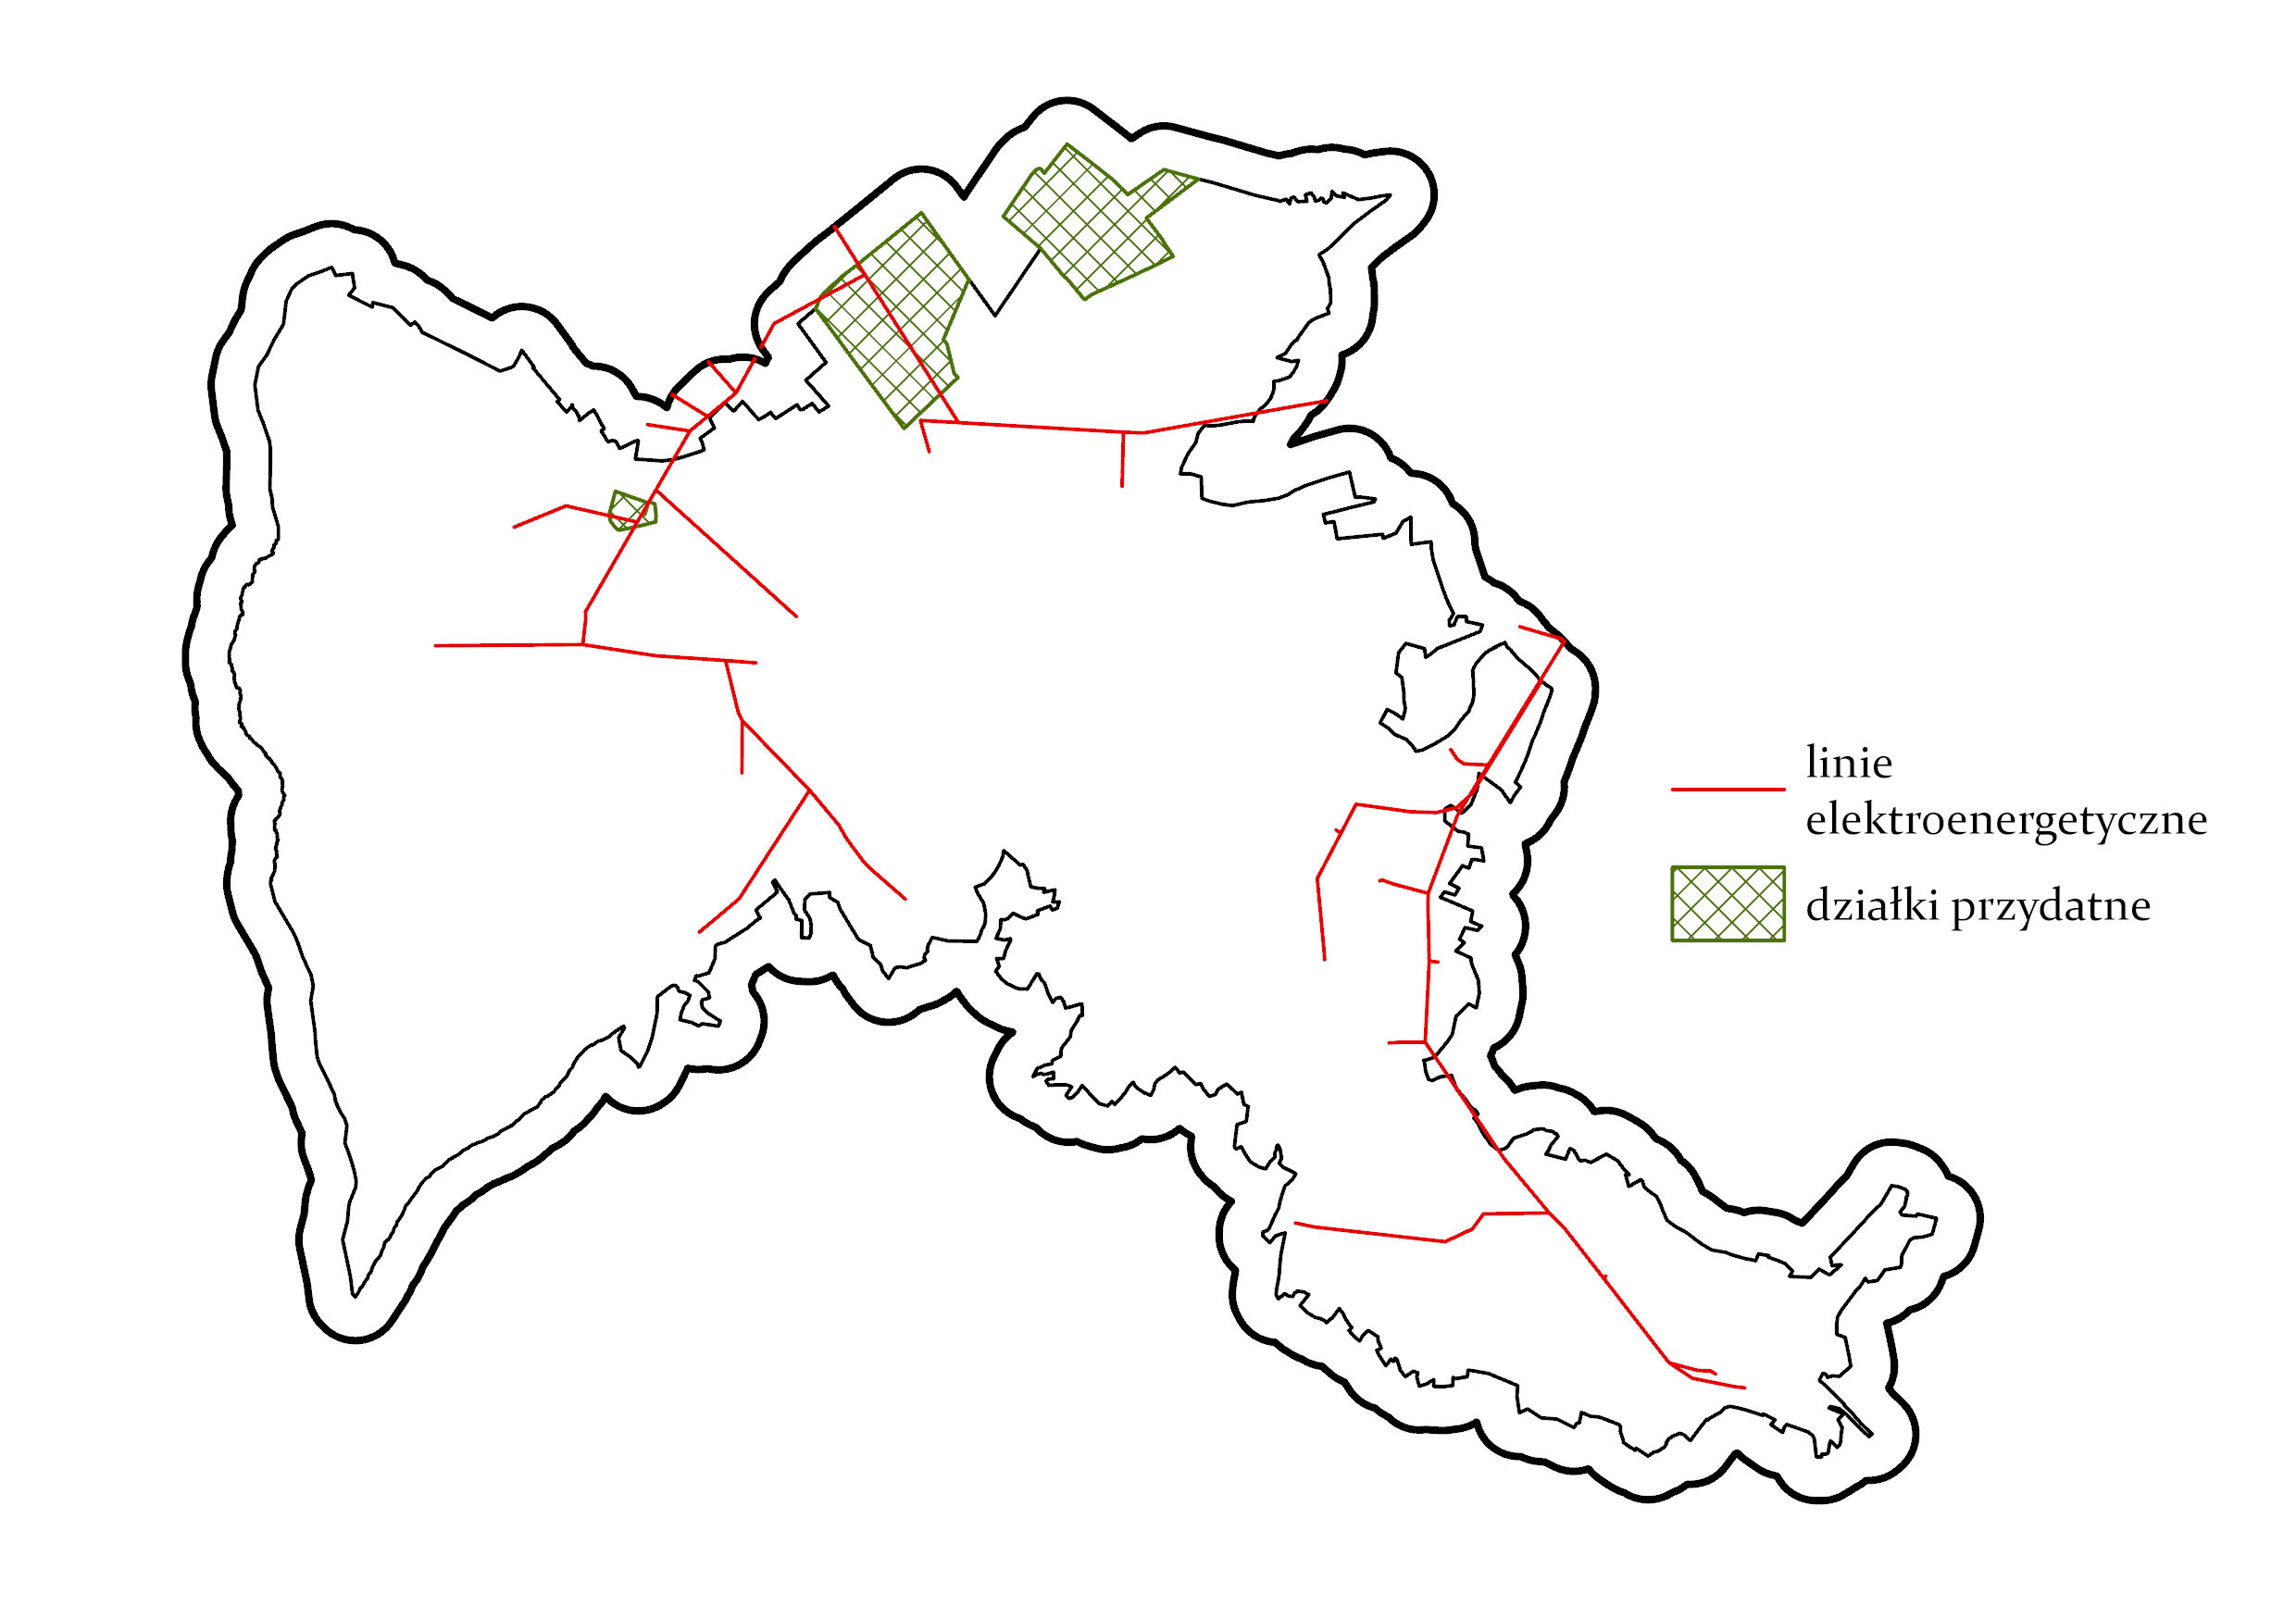
\includegraphics[width=0.75\textwidth]{img/dzialki-linie.jpg}
    \caption*{Mapa przedstawiająca przydatne działki oraz linie elektroenergetyczne}
\end{figure}

\subsubsection{Ostateczny wybór działki}

\section{Test modelu na danych z innego obszaru}
\subsection{Opis obszaru}
Stworzony model należało przetestować na innym obszarze. Wybrano do tego celu gminę Pleśna - wiejską gminę w powiecie tarnowskim w województwie małopolskim.

\begin{figure}[H]
    \centering
    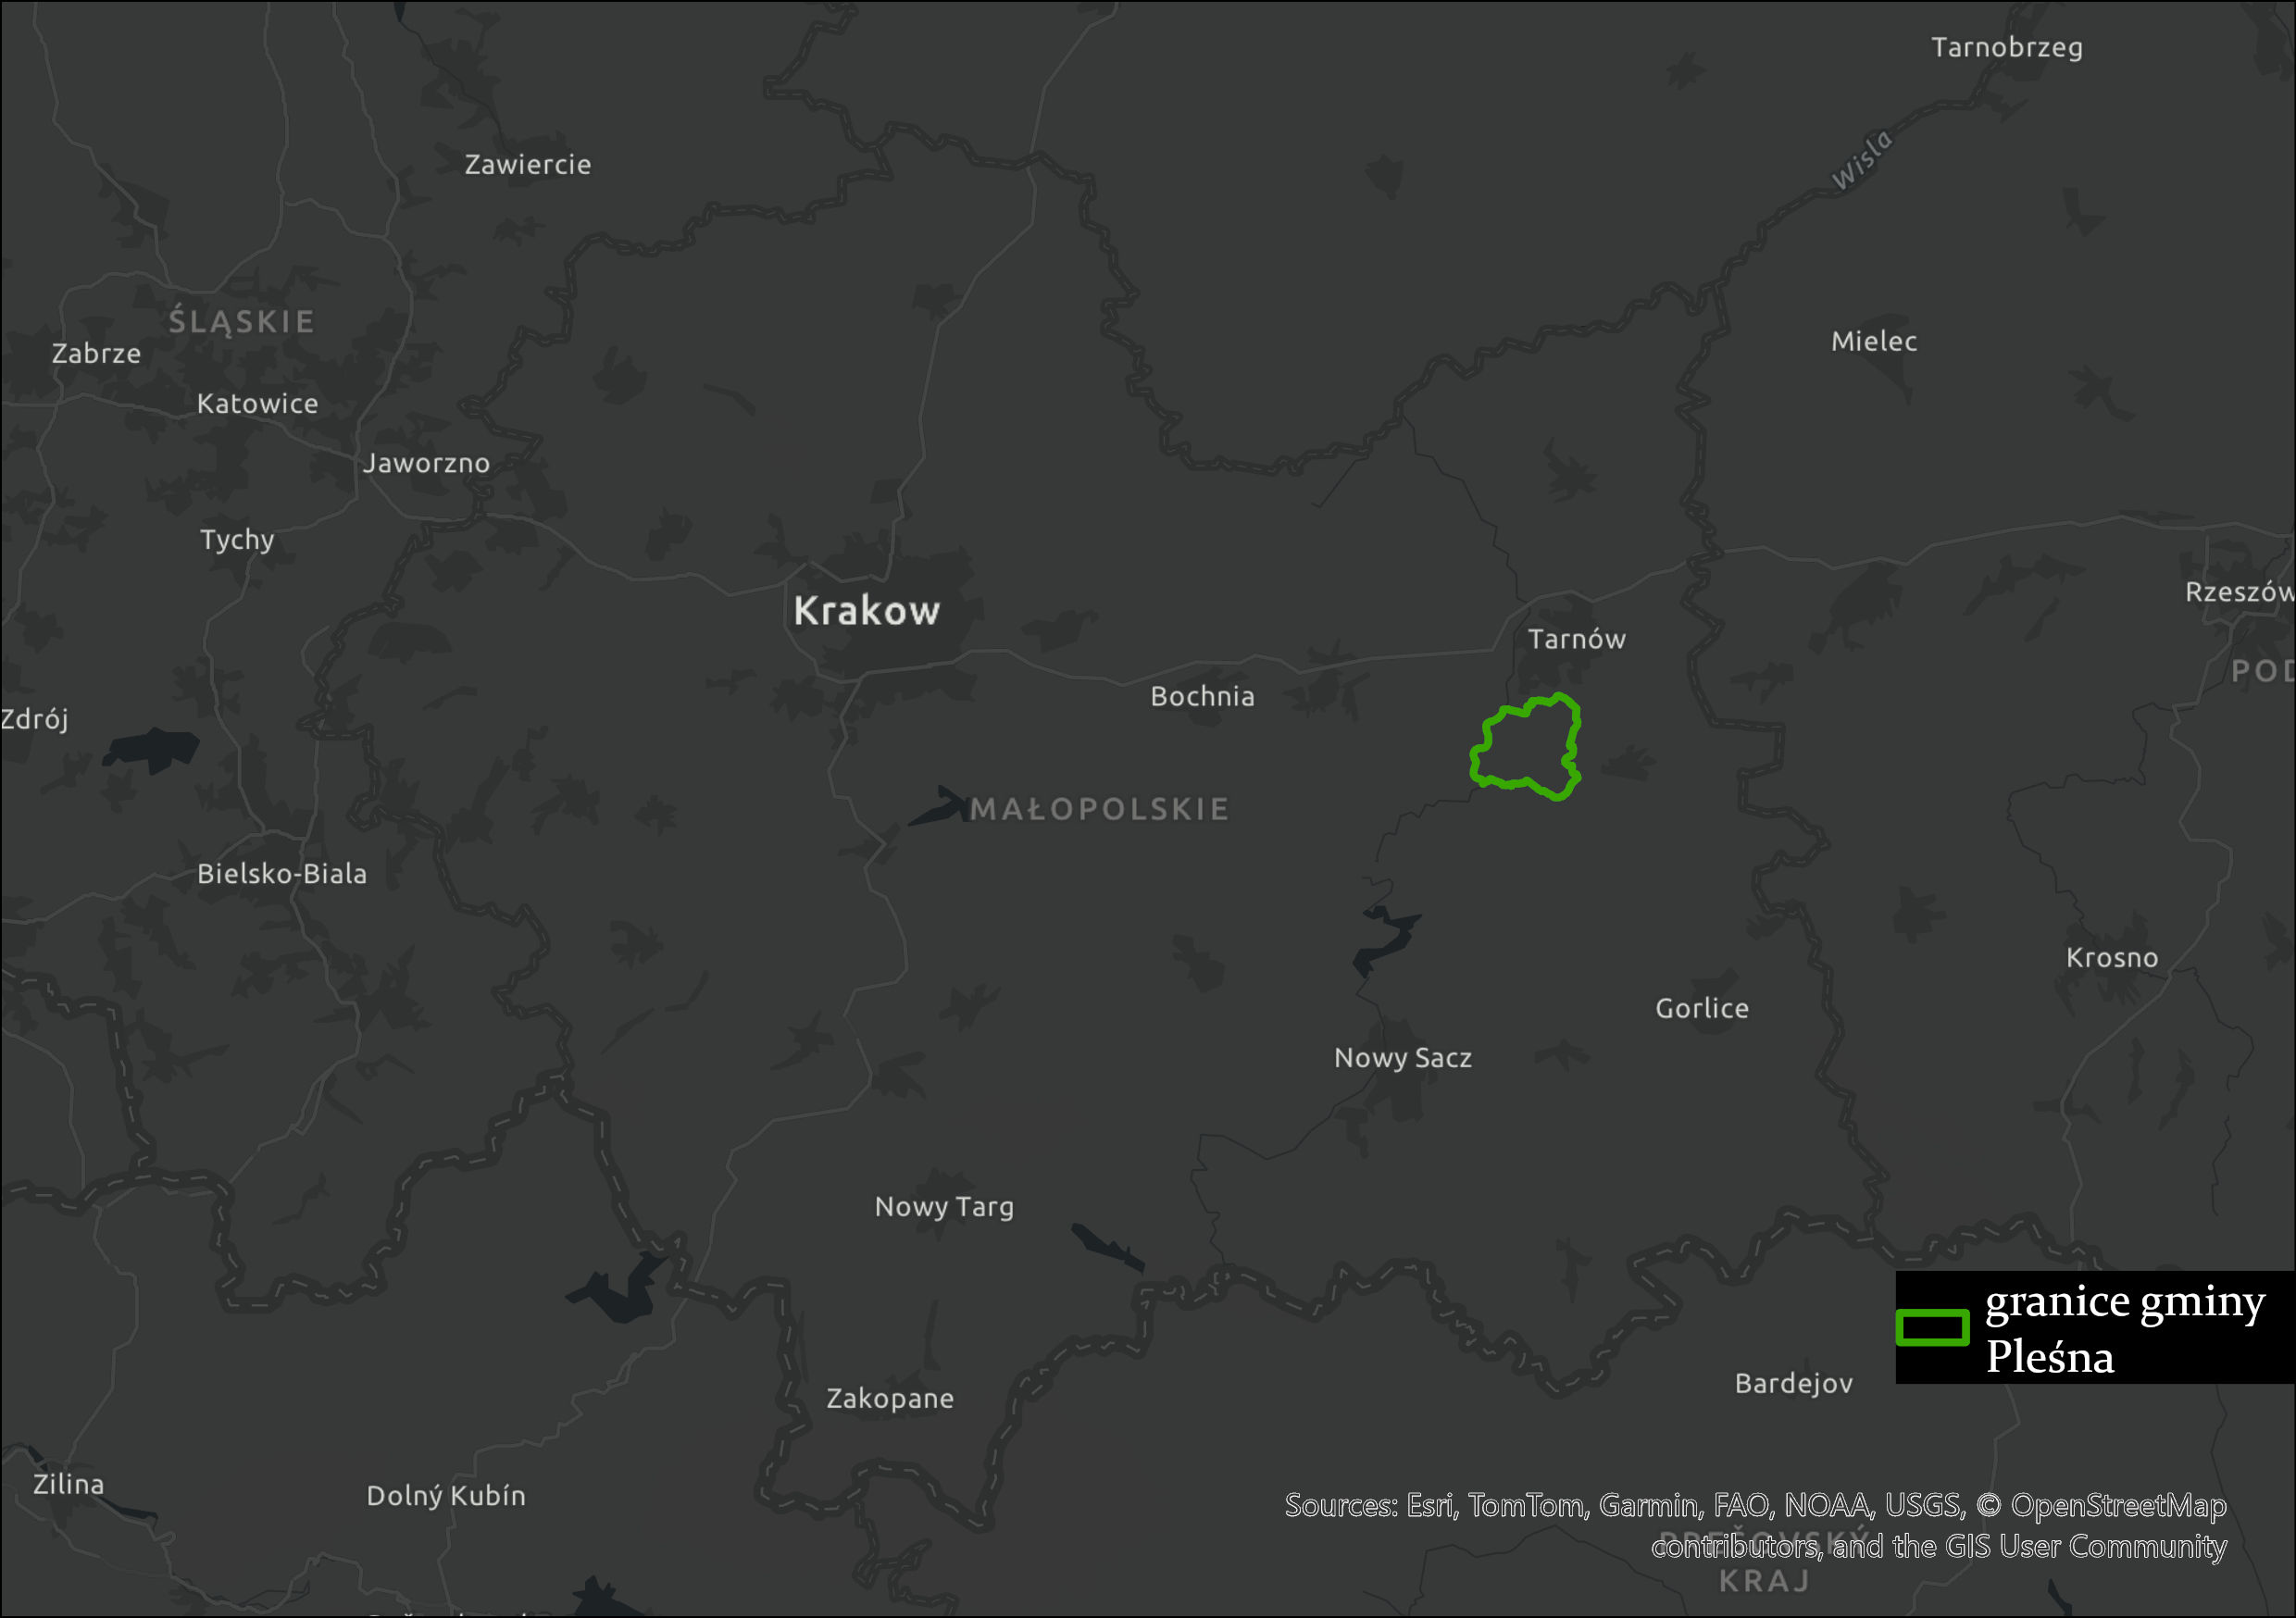
\includegraphics[width=0.75\textwidth]{img/plesna-polozenie.jpg}
    \caption*{Położenie gminy na mapie województwa małopolskiego}
\end{figure}

\subsection{Kryterium 1: odległość od rzek i zbiorników wodnych}
\begin{figure}[H]
    \centering
    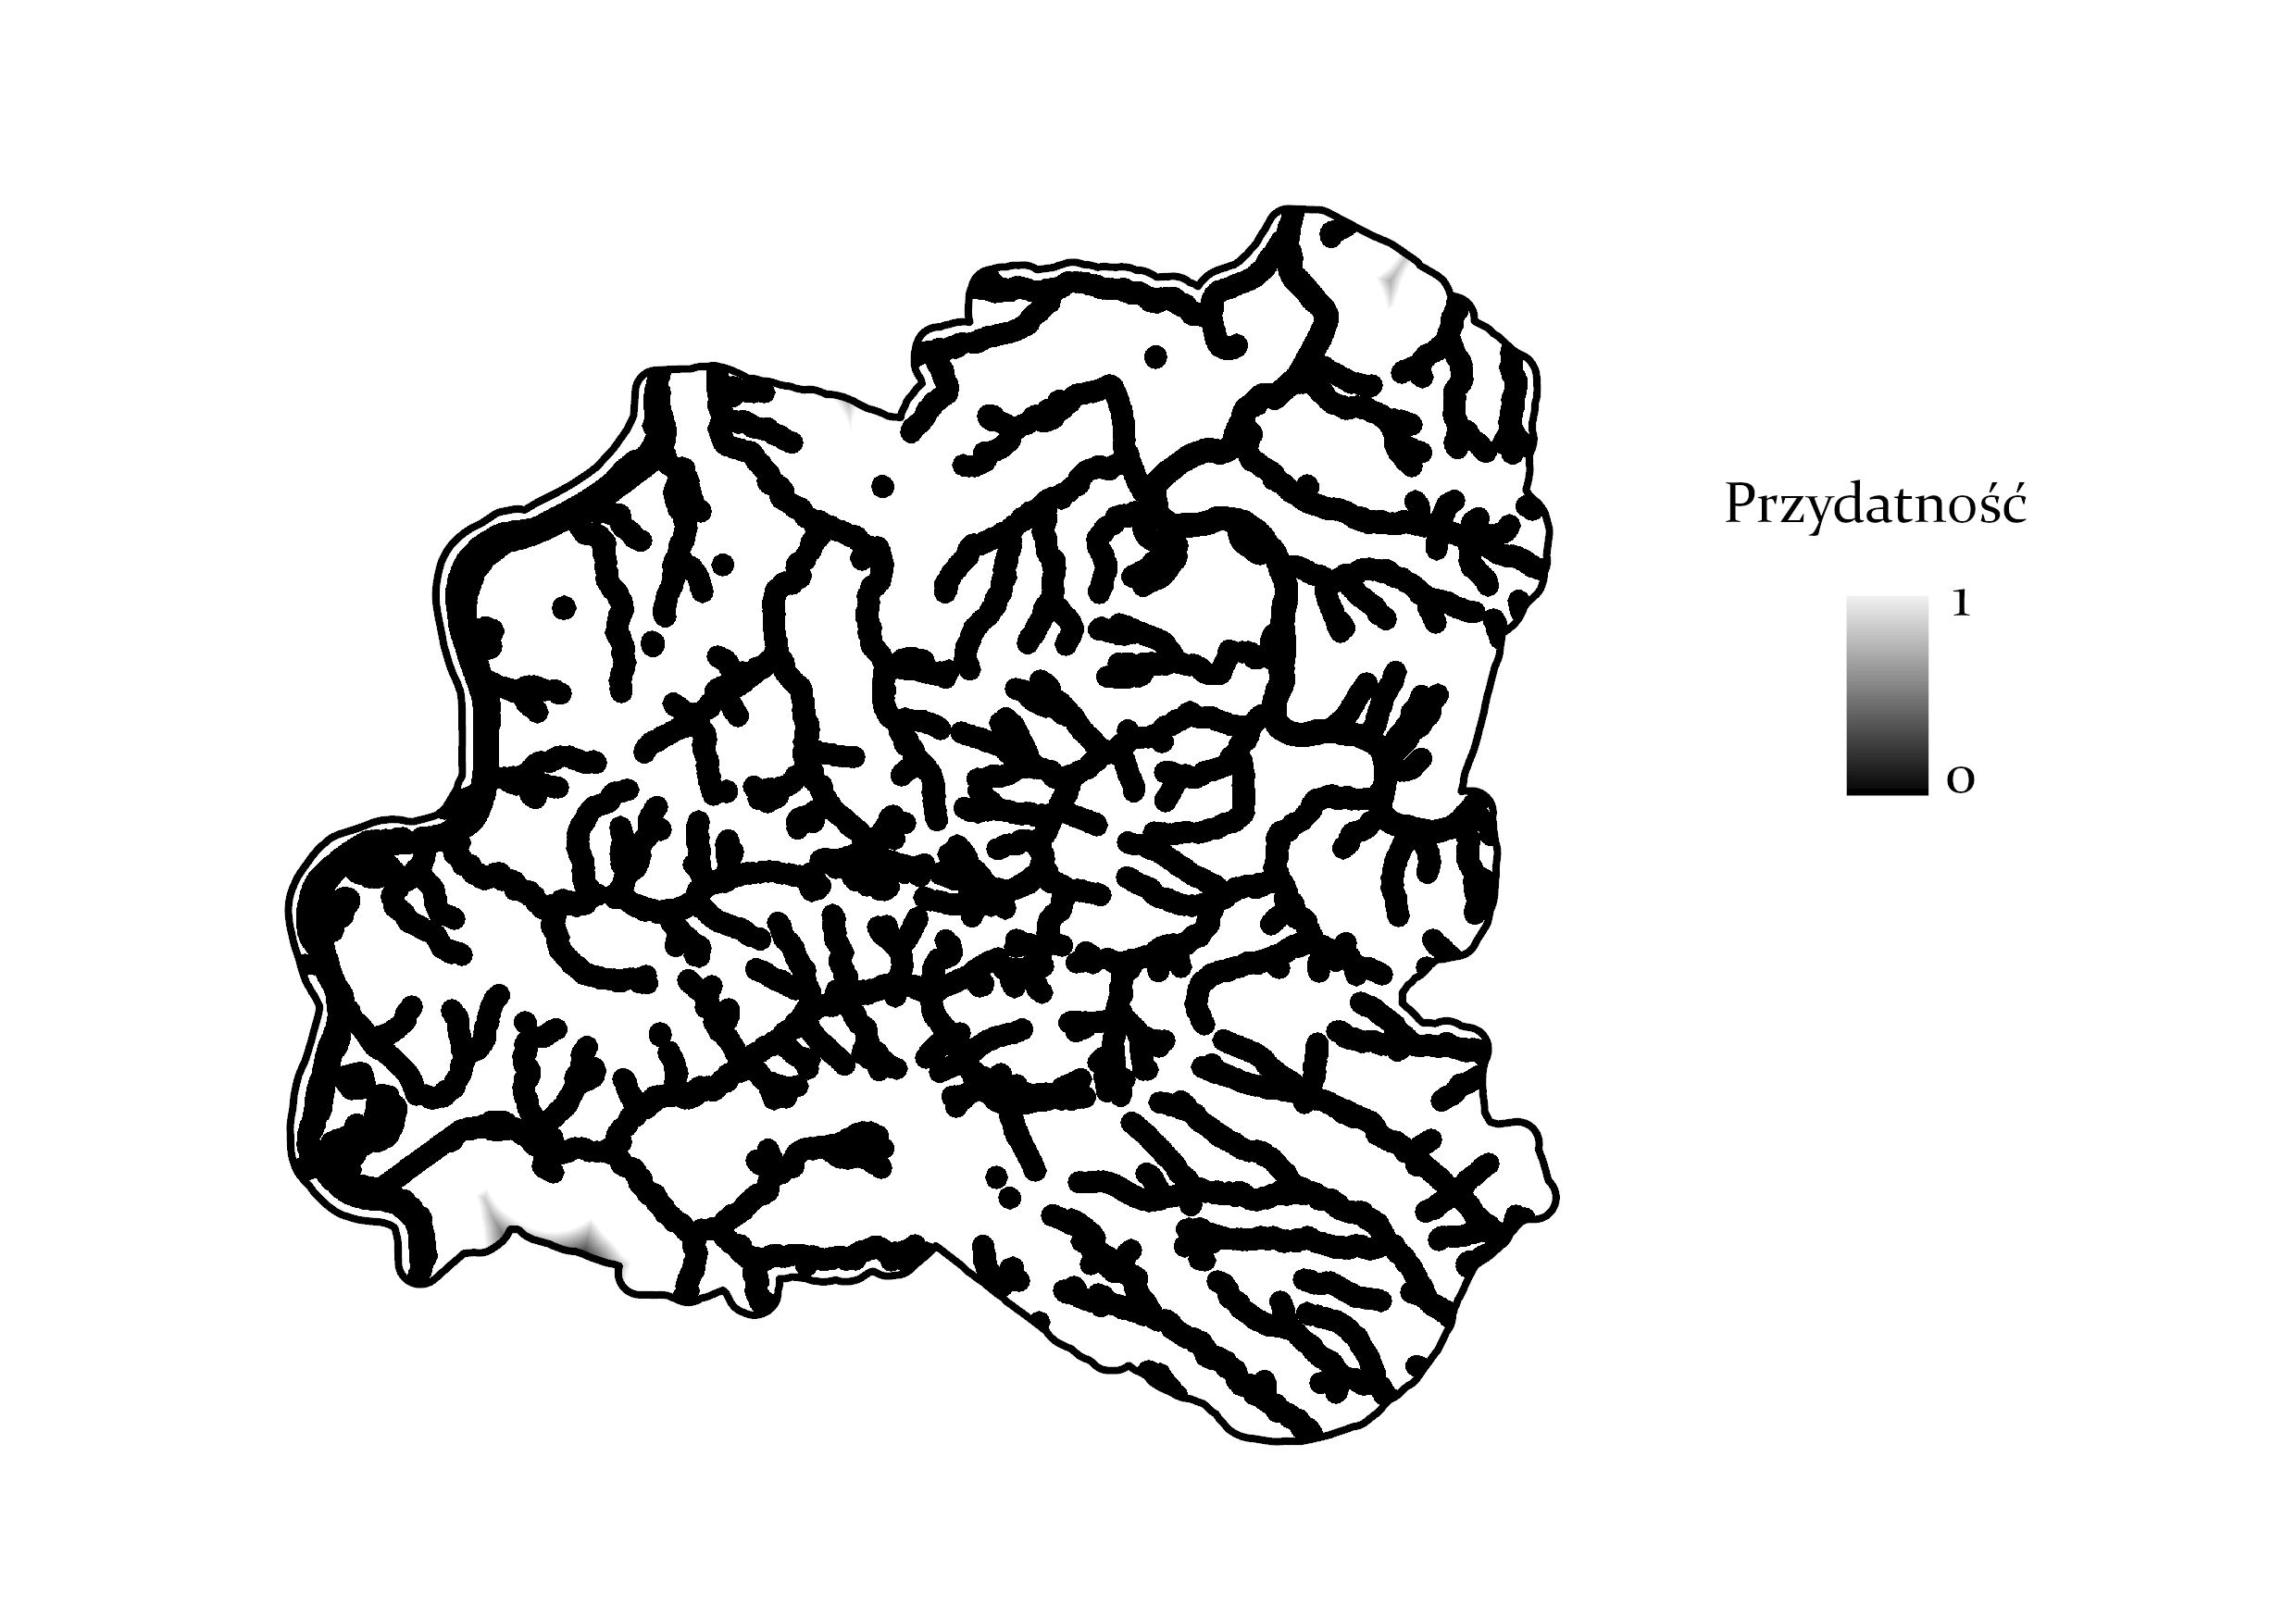
\includegraphics[width=0.75\textwidth]{img/plesna-kryterium1-layout.jpg}
    \caption*{Mapa przydatności dla kryterium 1.}
\end{figure}

\begin{figure}[H]
    \centering
    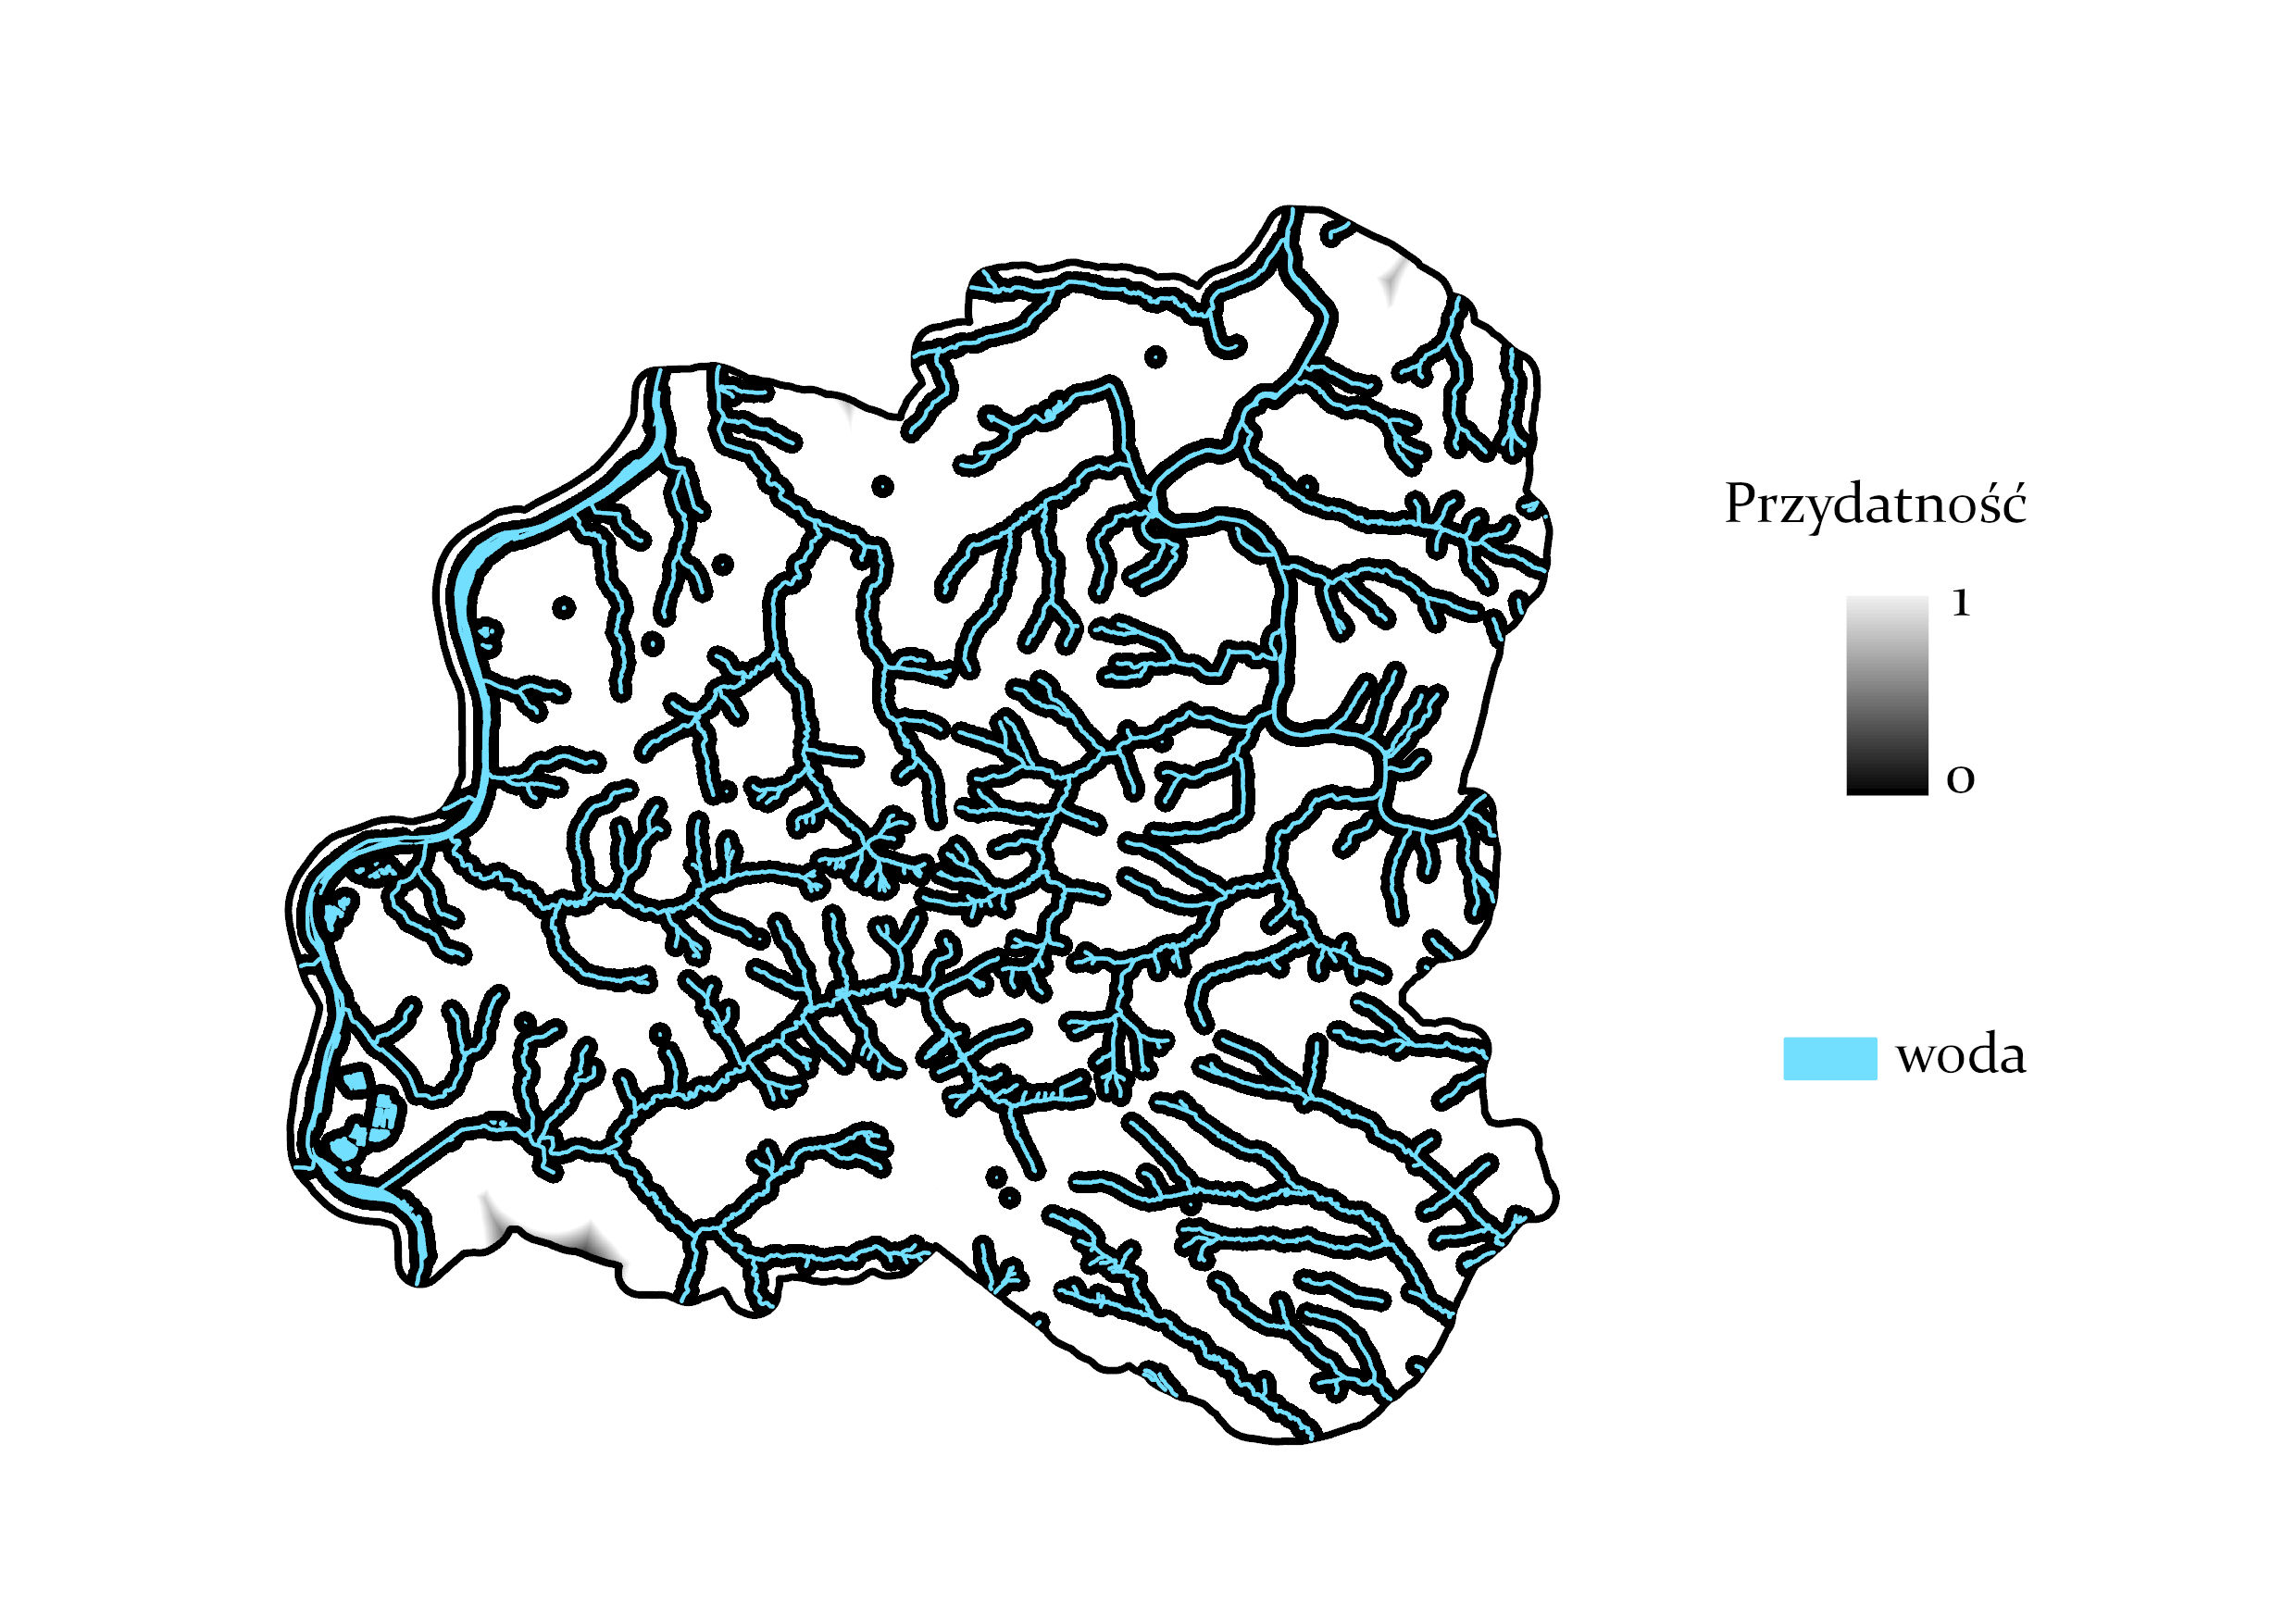
\includegraphics[width=0.75\textwidth]{img/plesna-kryterium1-woda.jpg}
    \caption*{Mapa przydatności dla kryterium 1. zawierająca rzeki oraz zbiorniki wodne}
\end{figure}

\subsection{Kryterium 2: odległość od budynków mieszkalnych}
\begin{figure}[H]
    \centering
    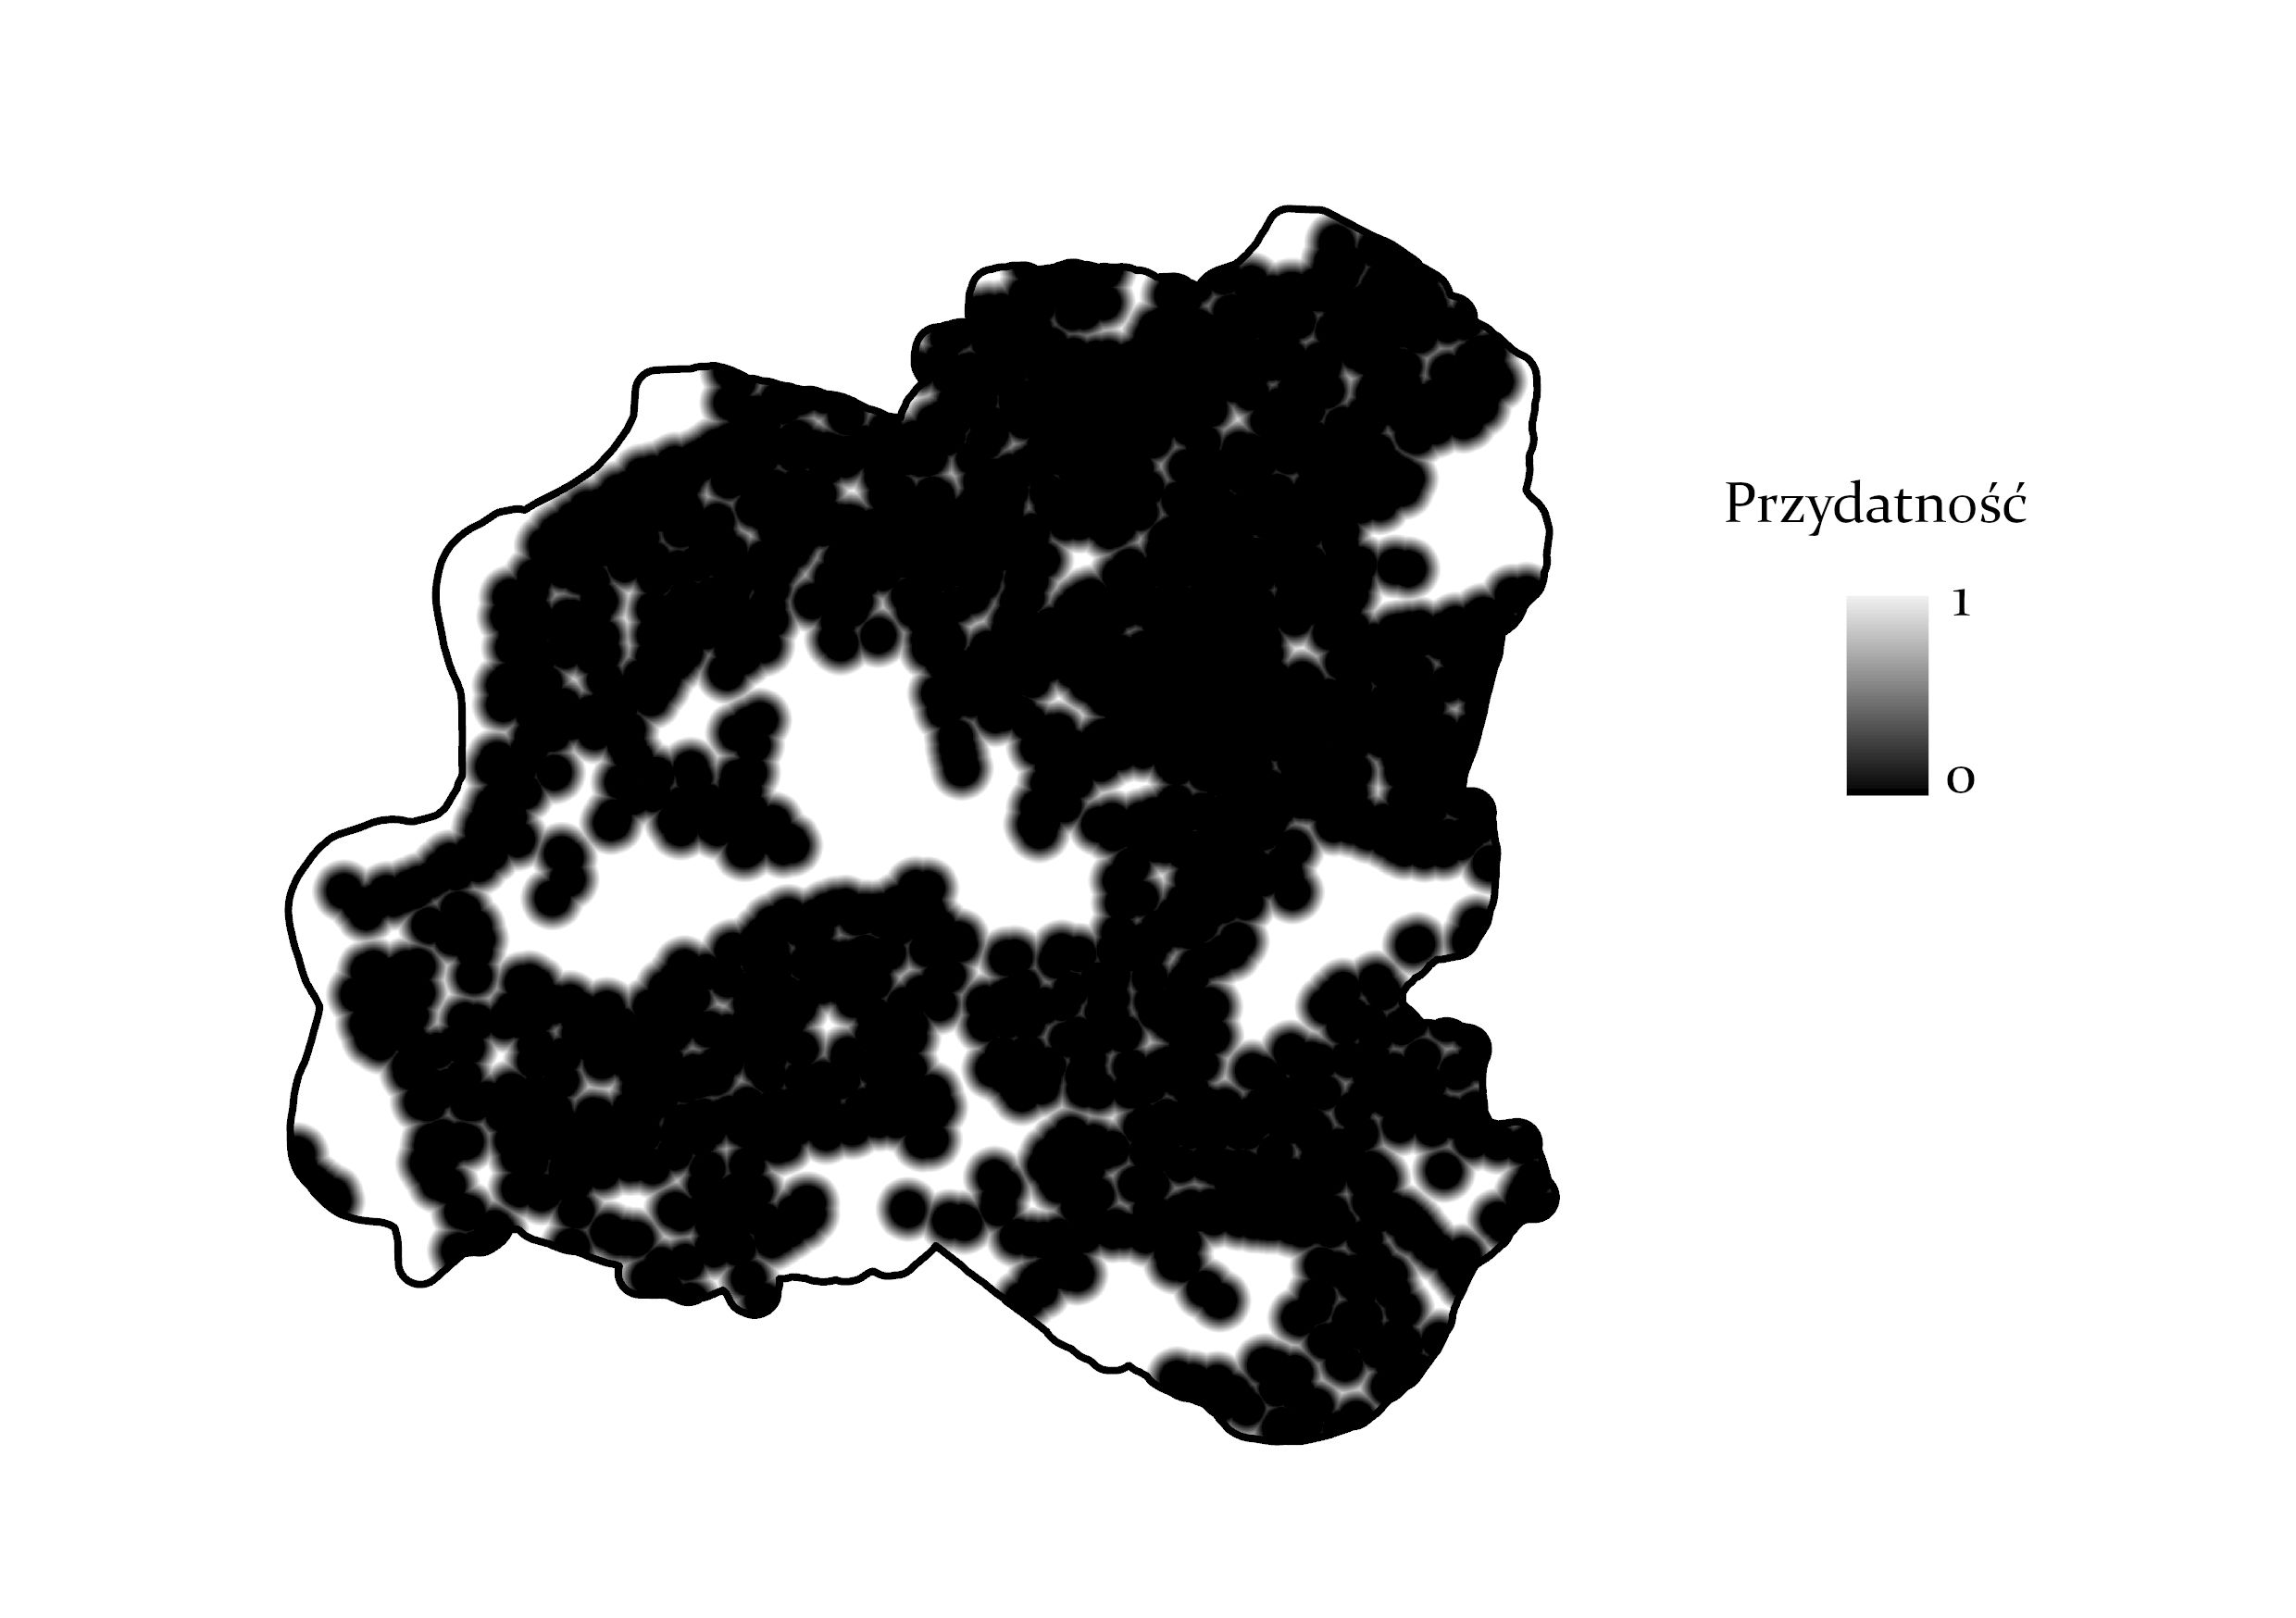
\includegraphics[width=0.75\textwidth]{img/plesna-kryterium2-layout.jpg}
    \caption*{Mapa przydatności dla kryterium 2.}
\end{figure}

\begin{figure}[H]
    \centering
    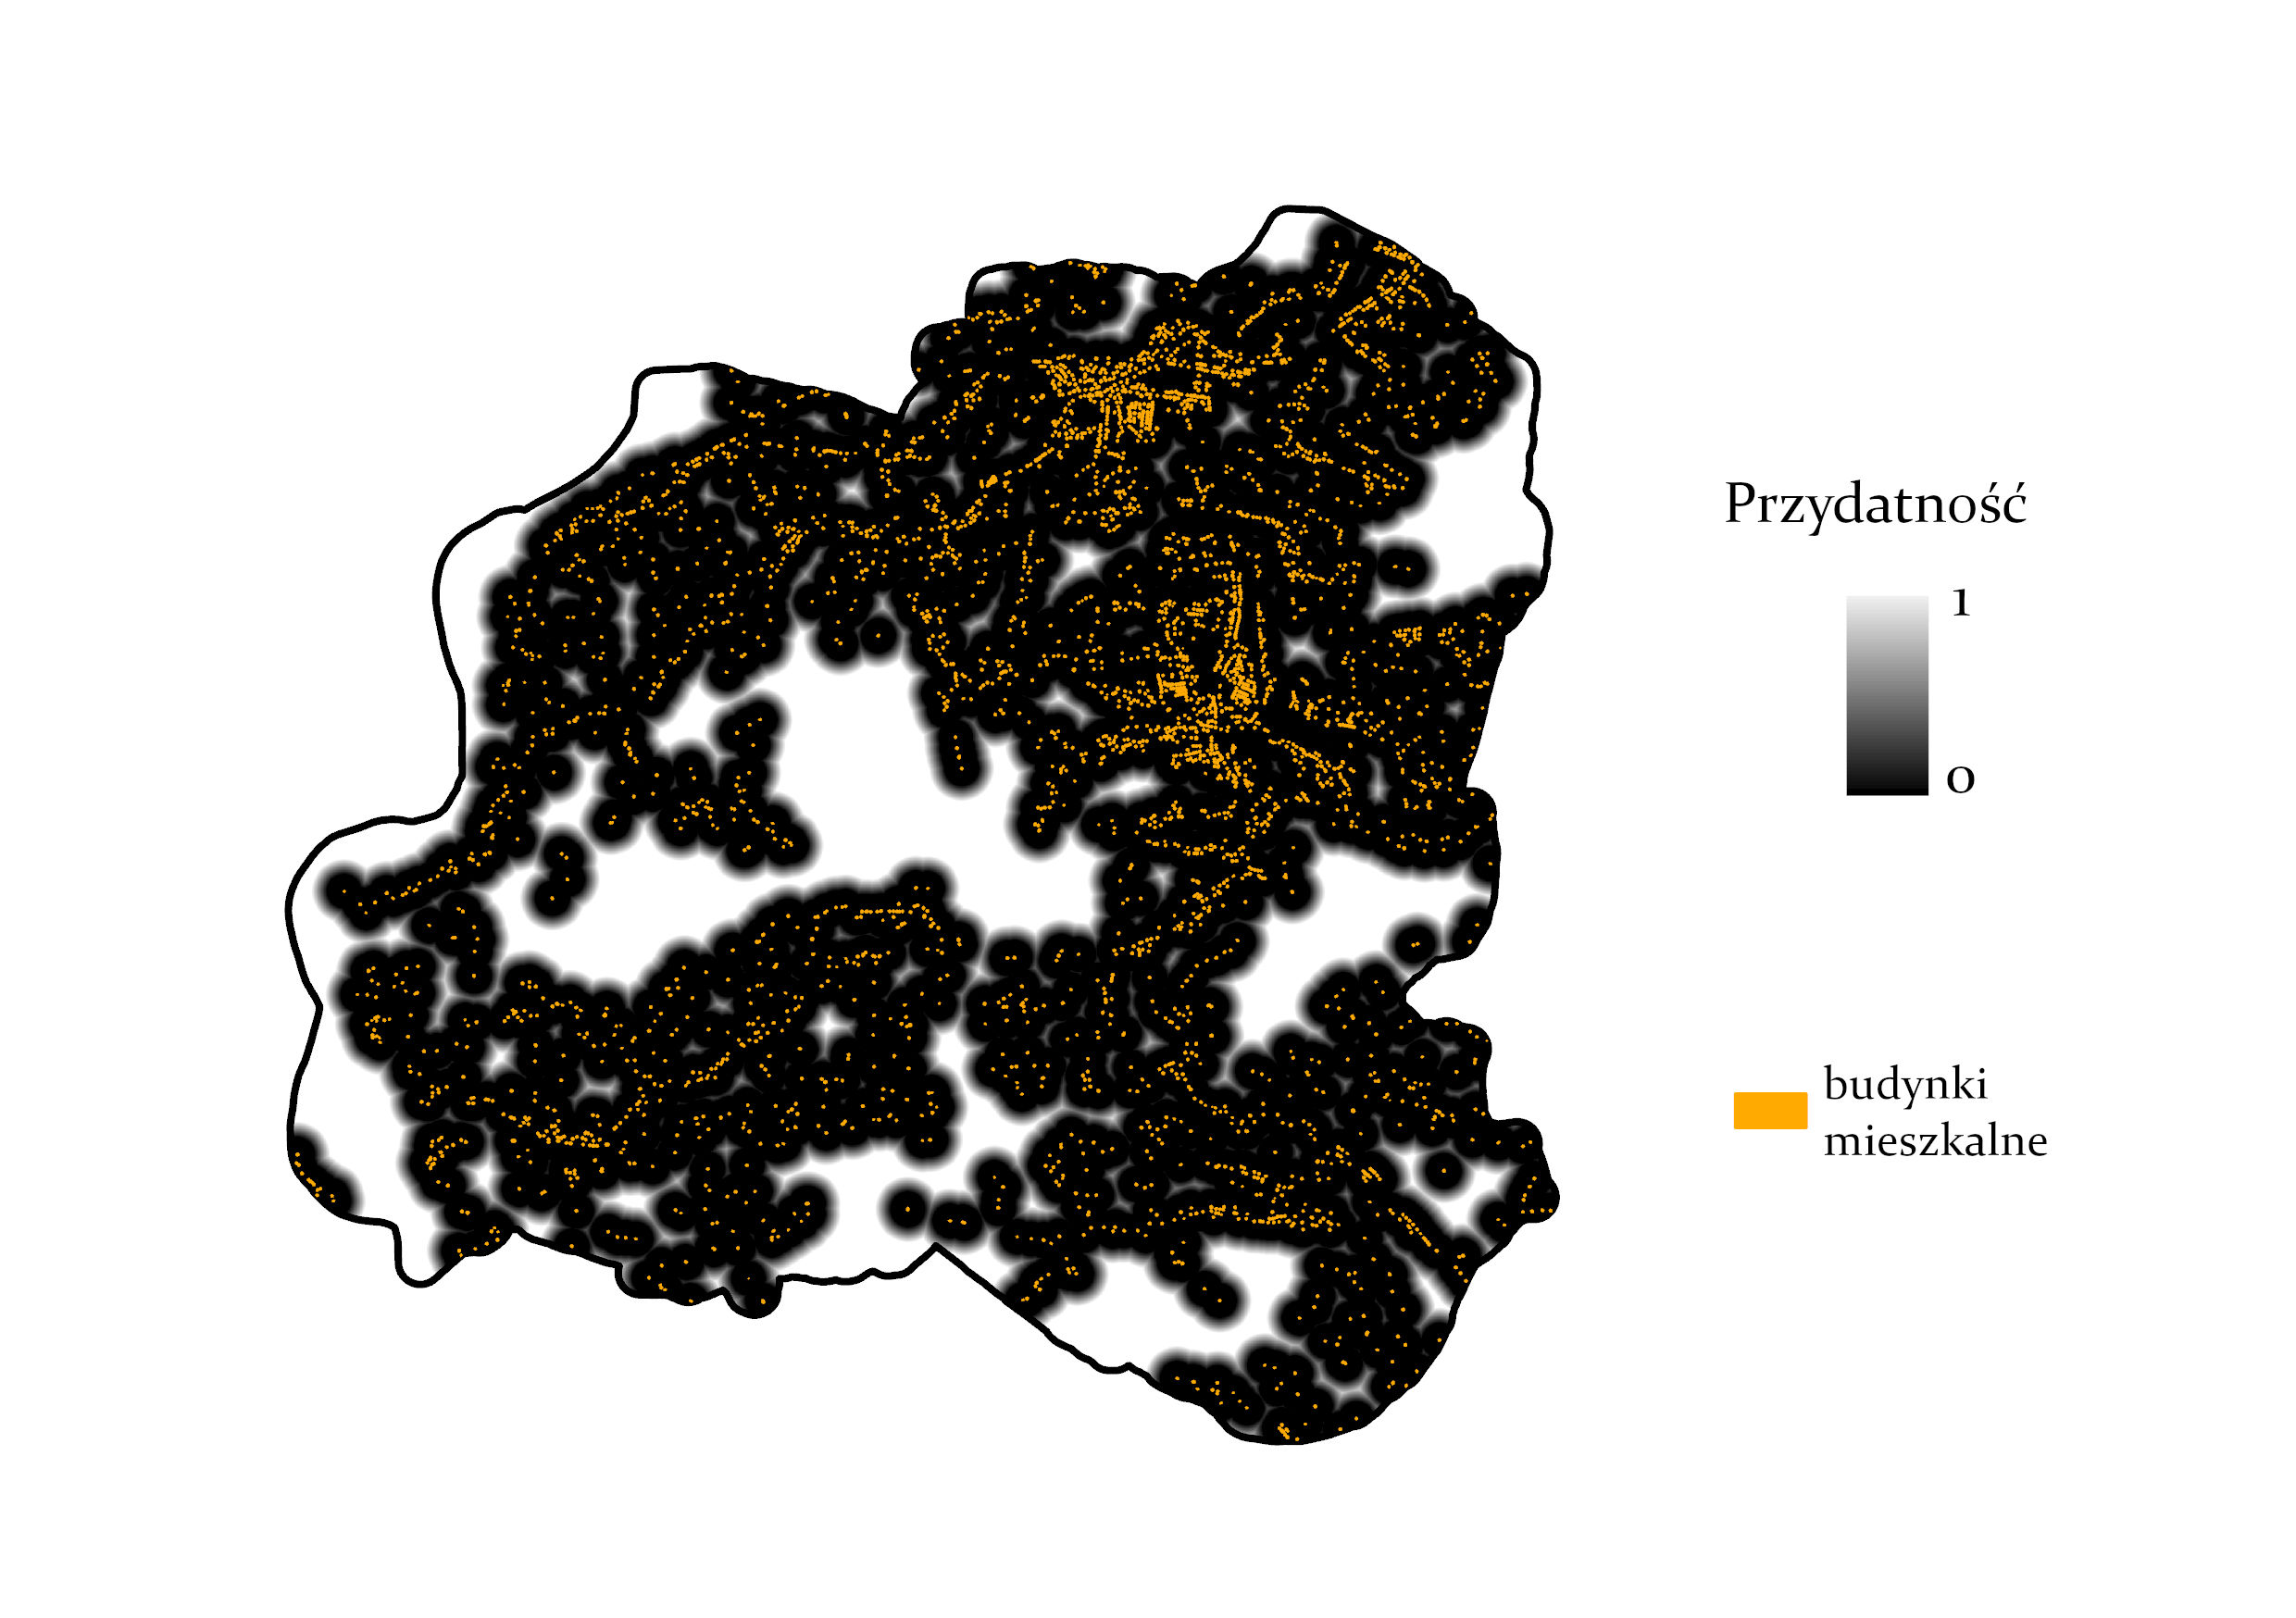
\includegraphics[width=0.75\textwidth]{img/plesna-kryterium2-budynki.jpg}
    \caption*{Mapa przydatności dla kryterium 2. zawierająca budynki mieszkalne}
\end{figure}

\subsection{Kryterium 3: pokrycie terenu}

\begin{figure}[H]
    \centering
    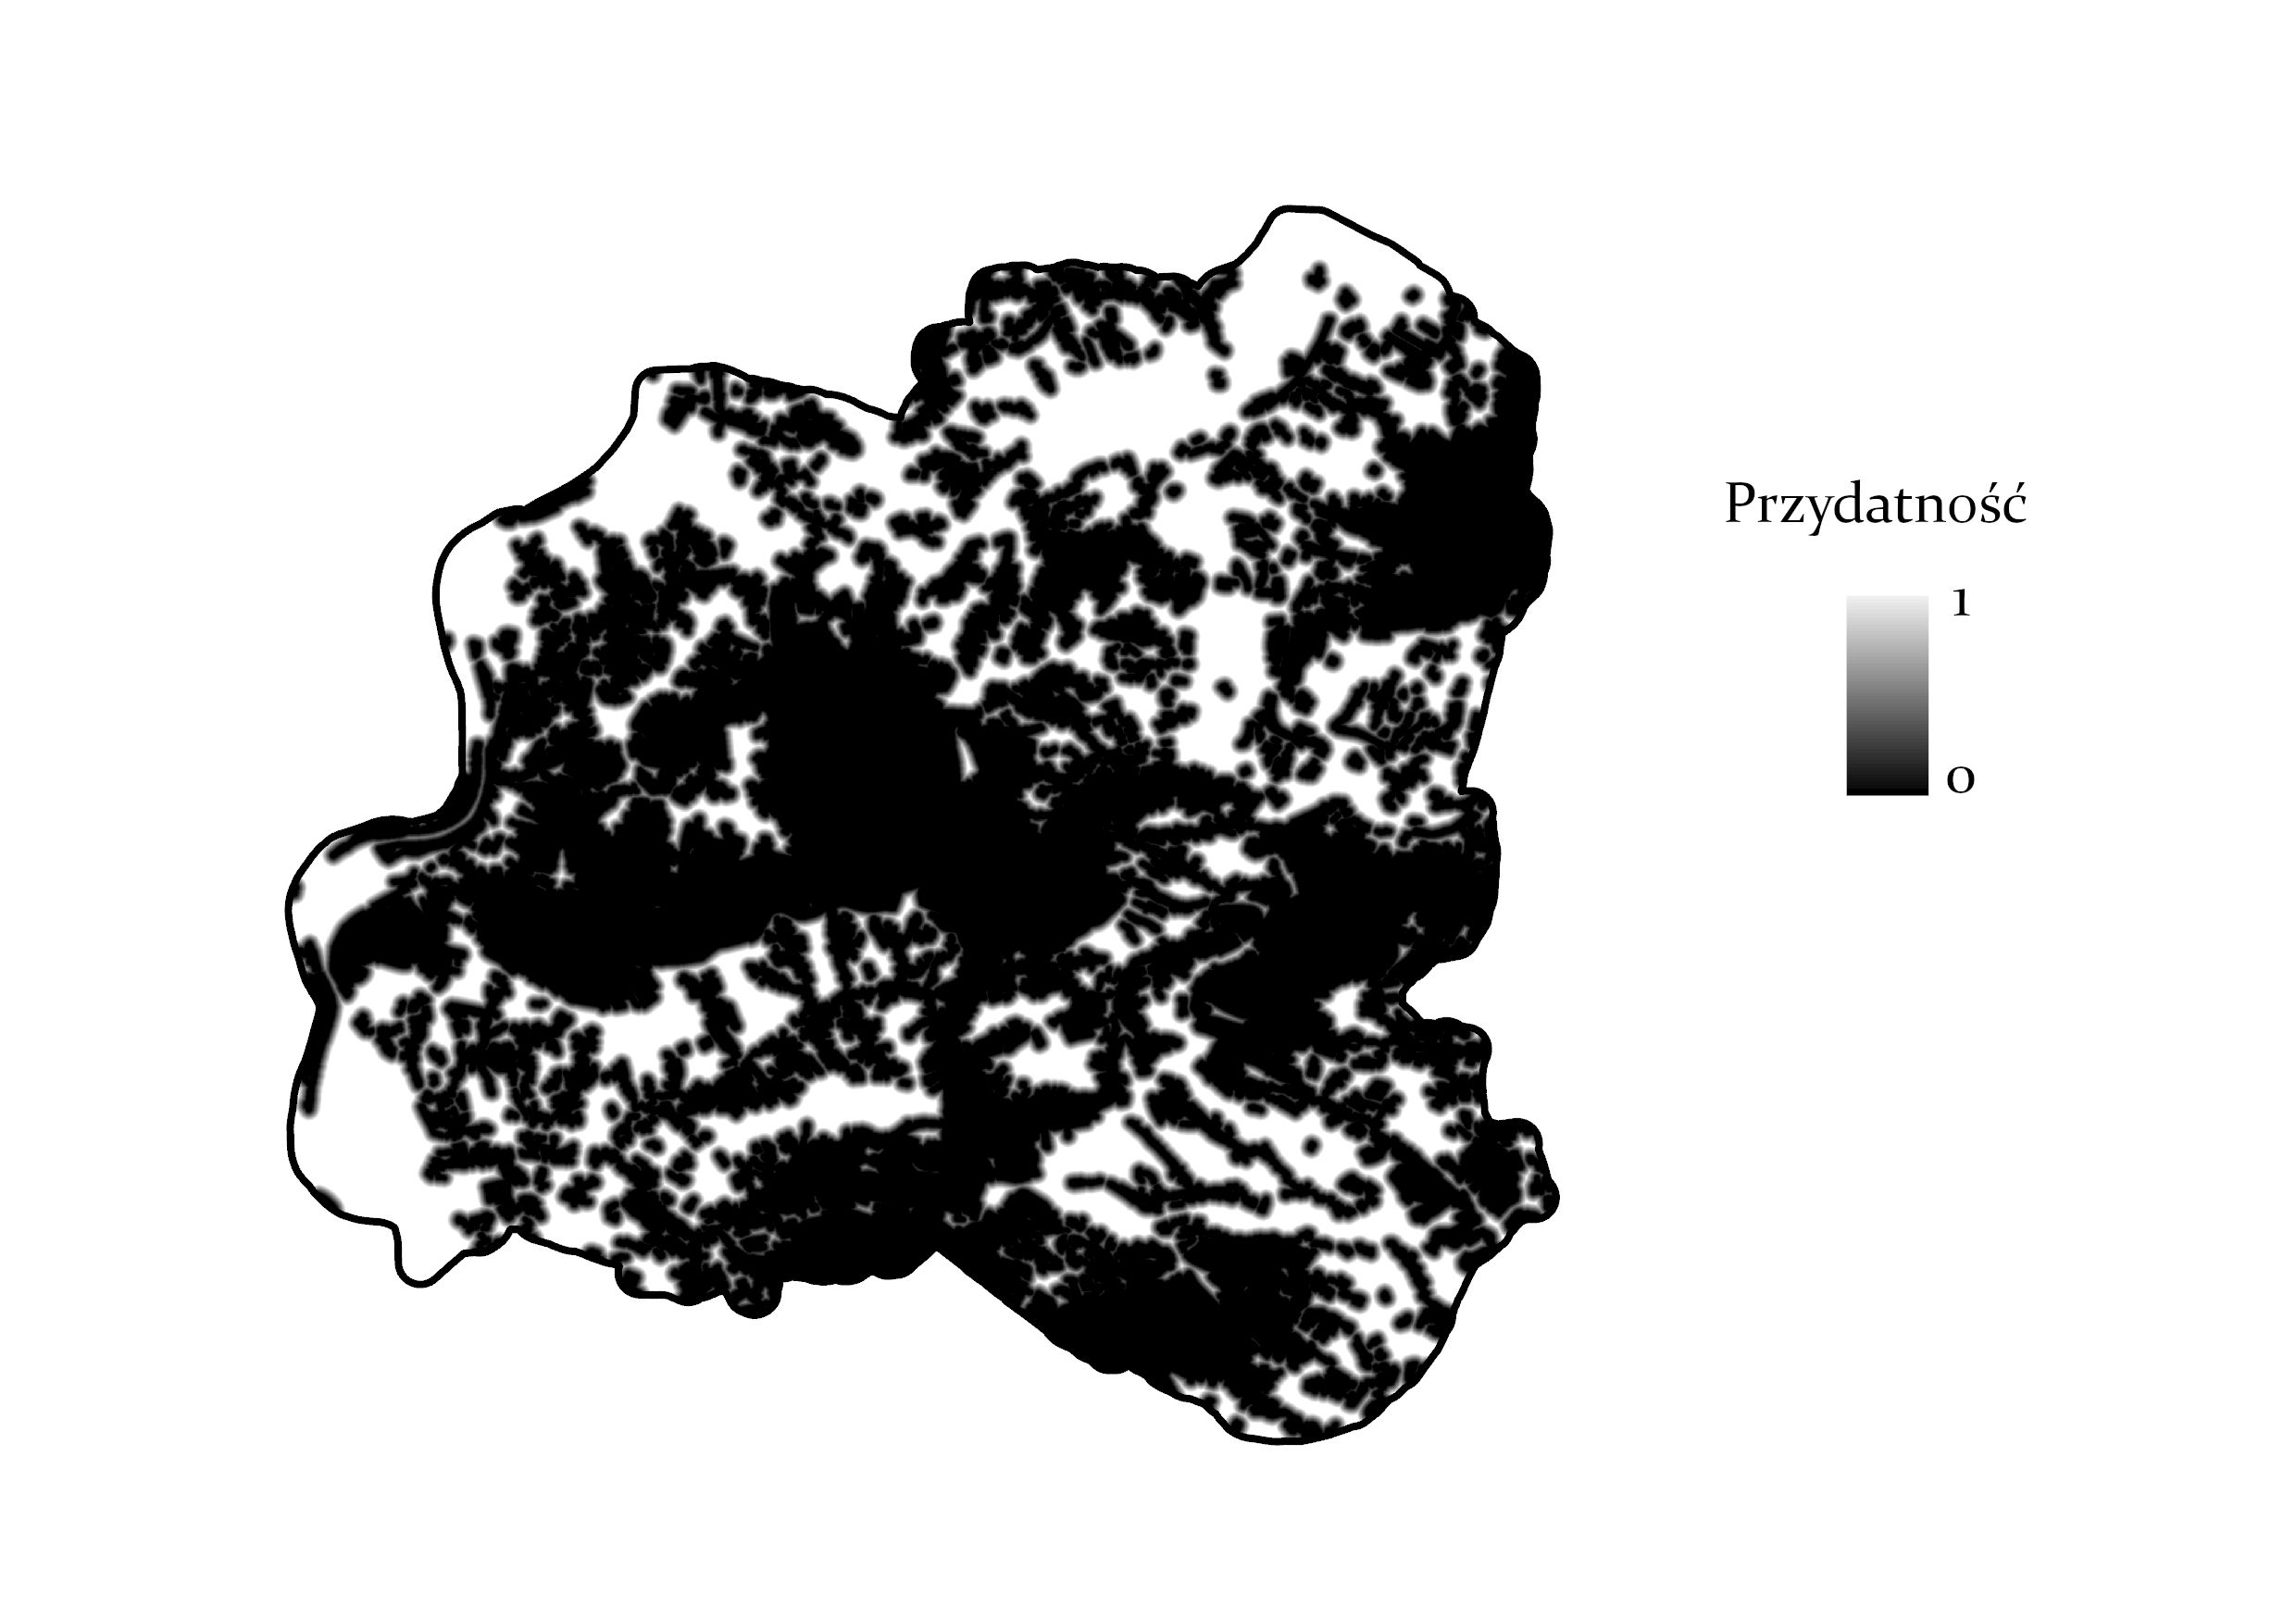
\includegraphics[width=0.75\textwidth]{img/plesna-kryterium3-layout.jpg}
    \caption*{Mapa przydatności dla kryterium 3.}
\end{figure}

\begin{figure}[H]
    \centering
    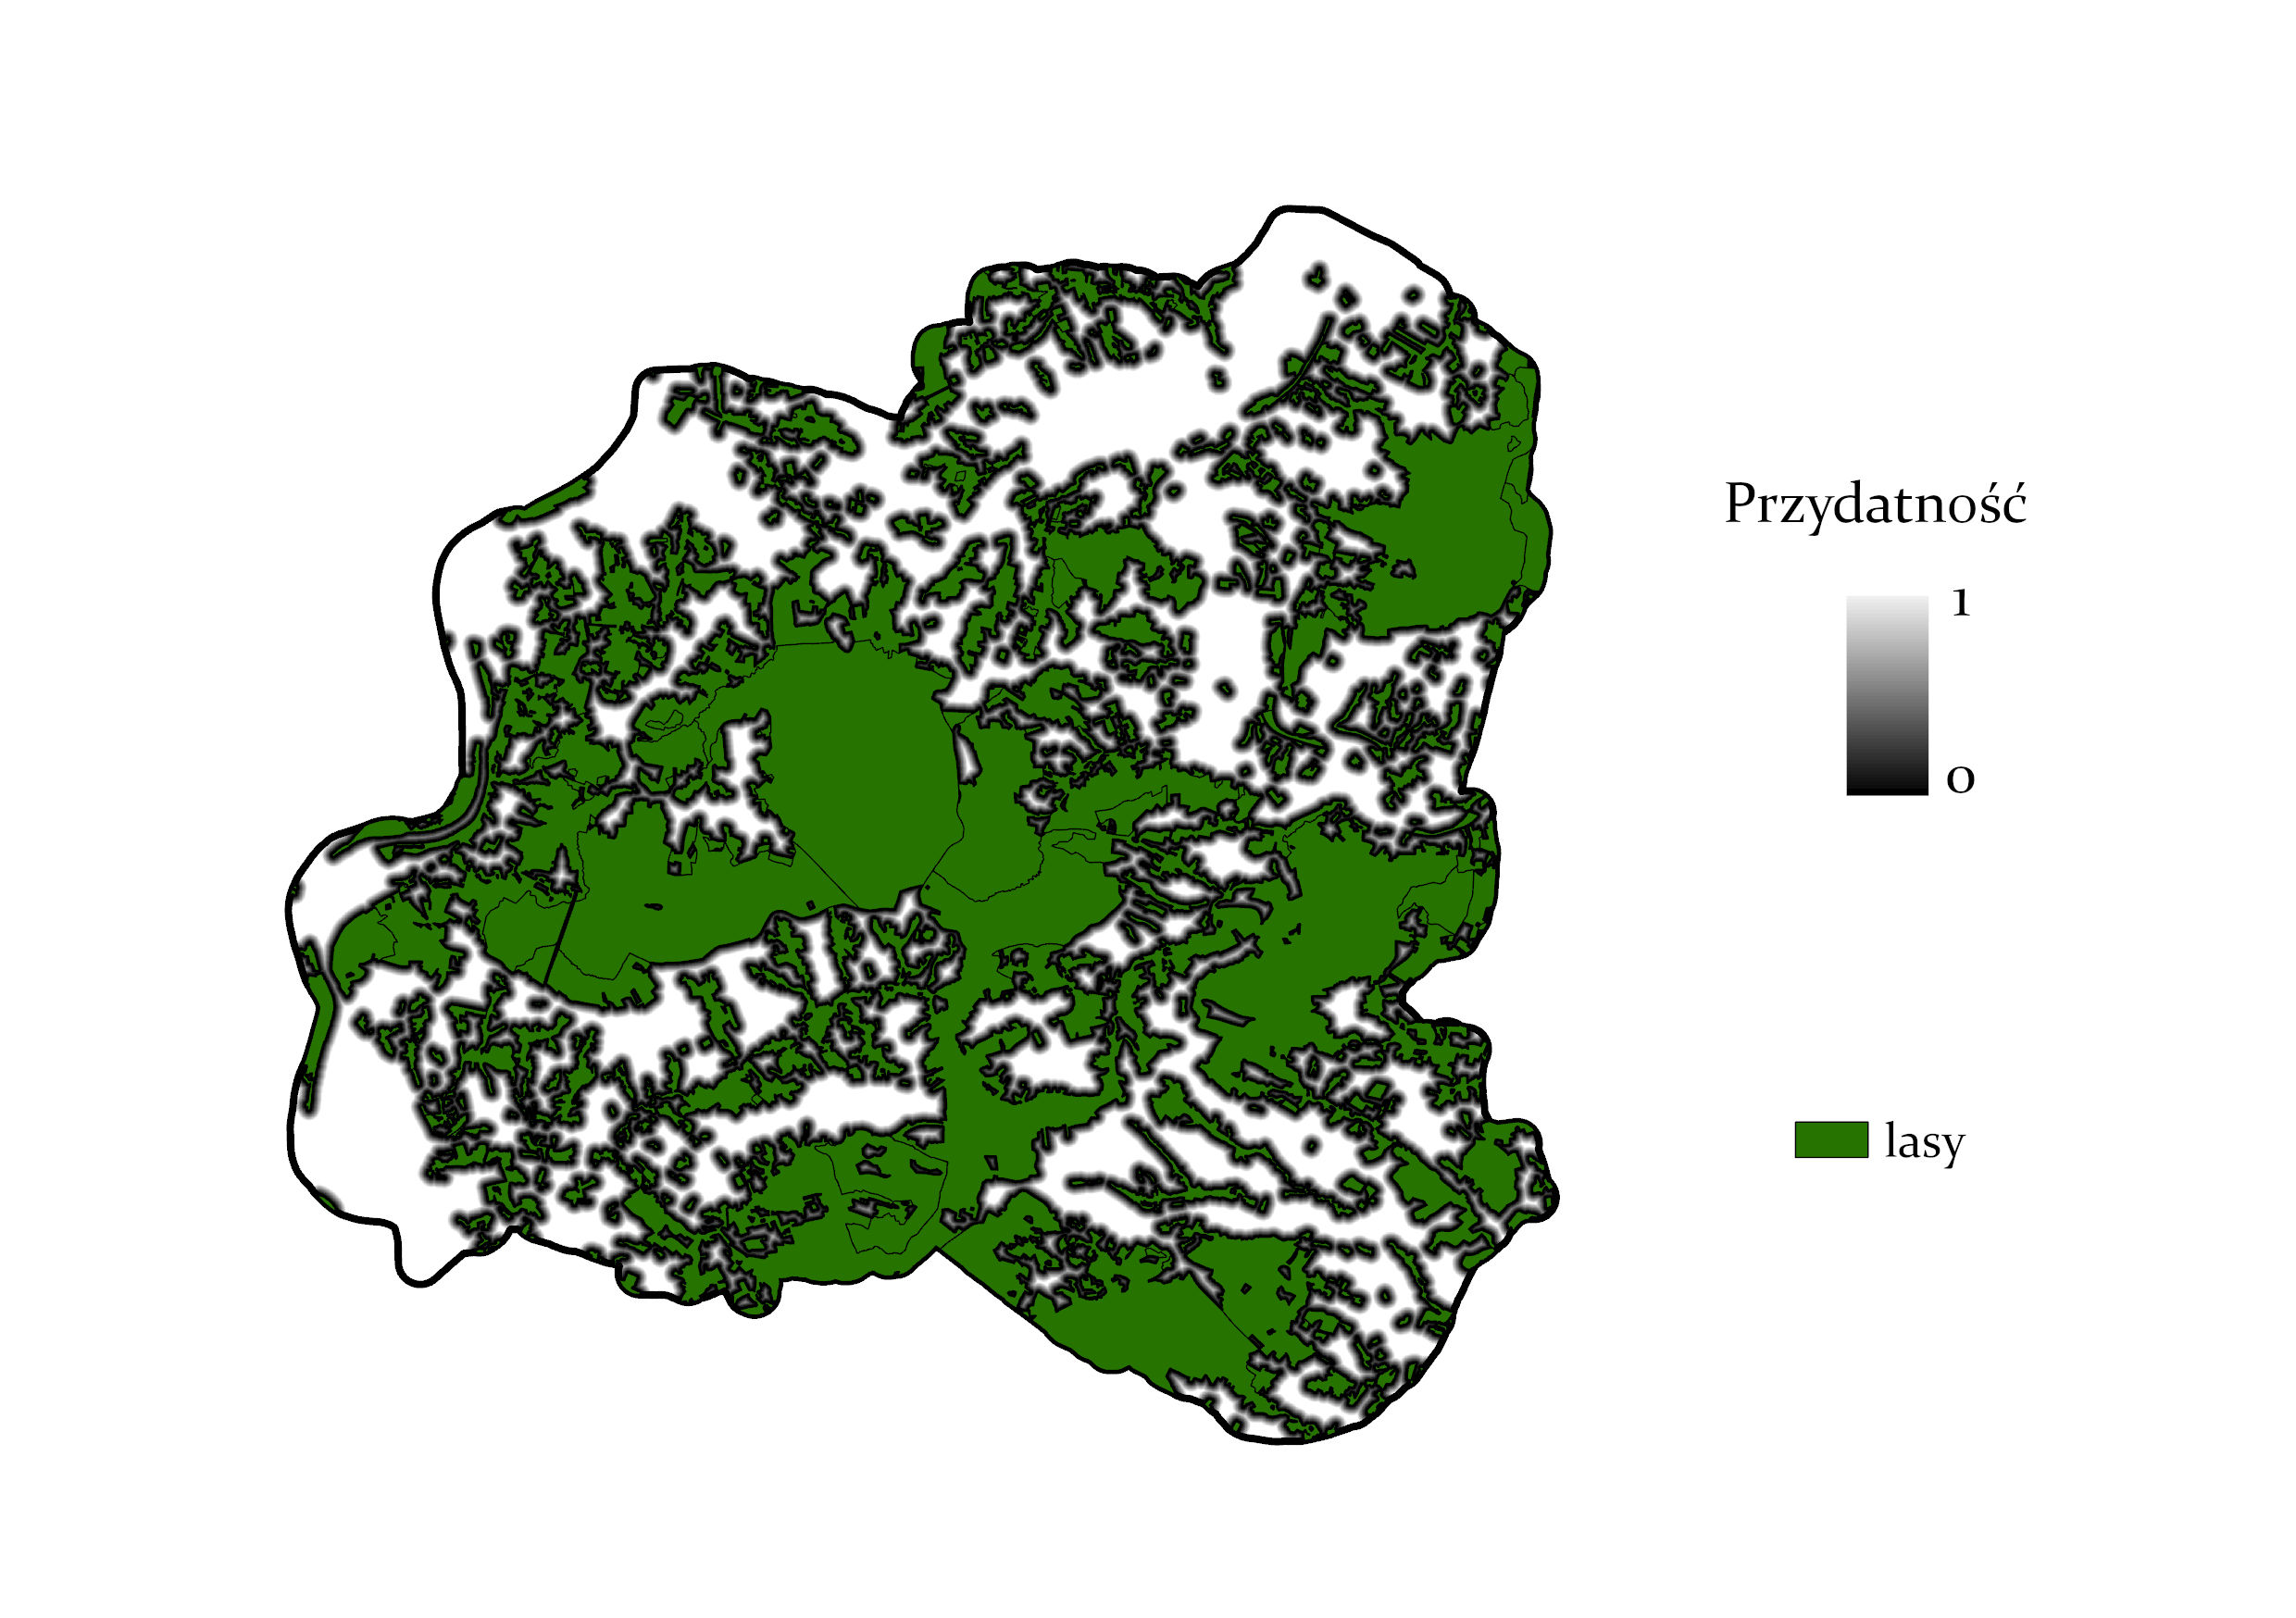
\includegraphics[width=0.75\textwidth]{img/plesna-kryterium3-lasy.jpg}
    \caption*{Mapa przydatności dla kryterium 3. zawierająca lasy}
\end{figure}

\subsection{Kryterium 4: dostęp do dróg utwardzonych}

\begin{figure}[H]
    \centering
    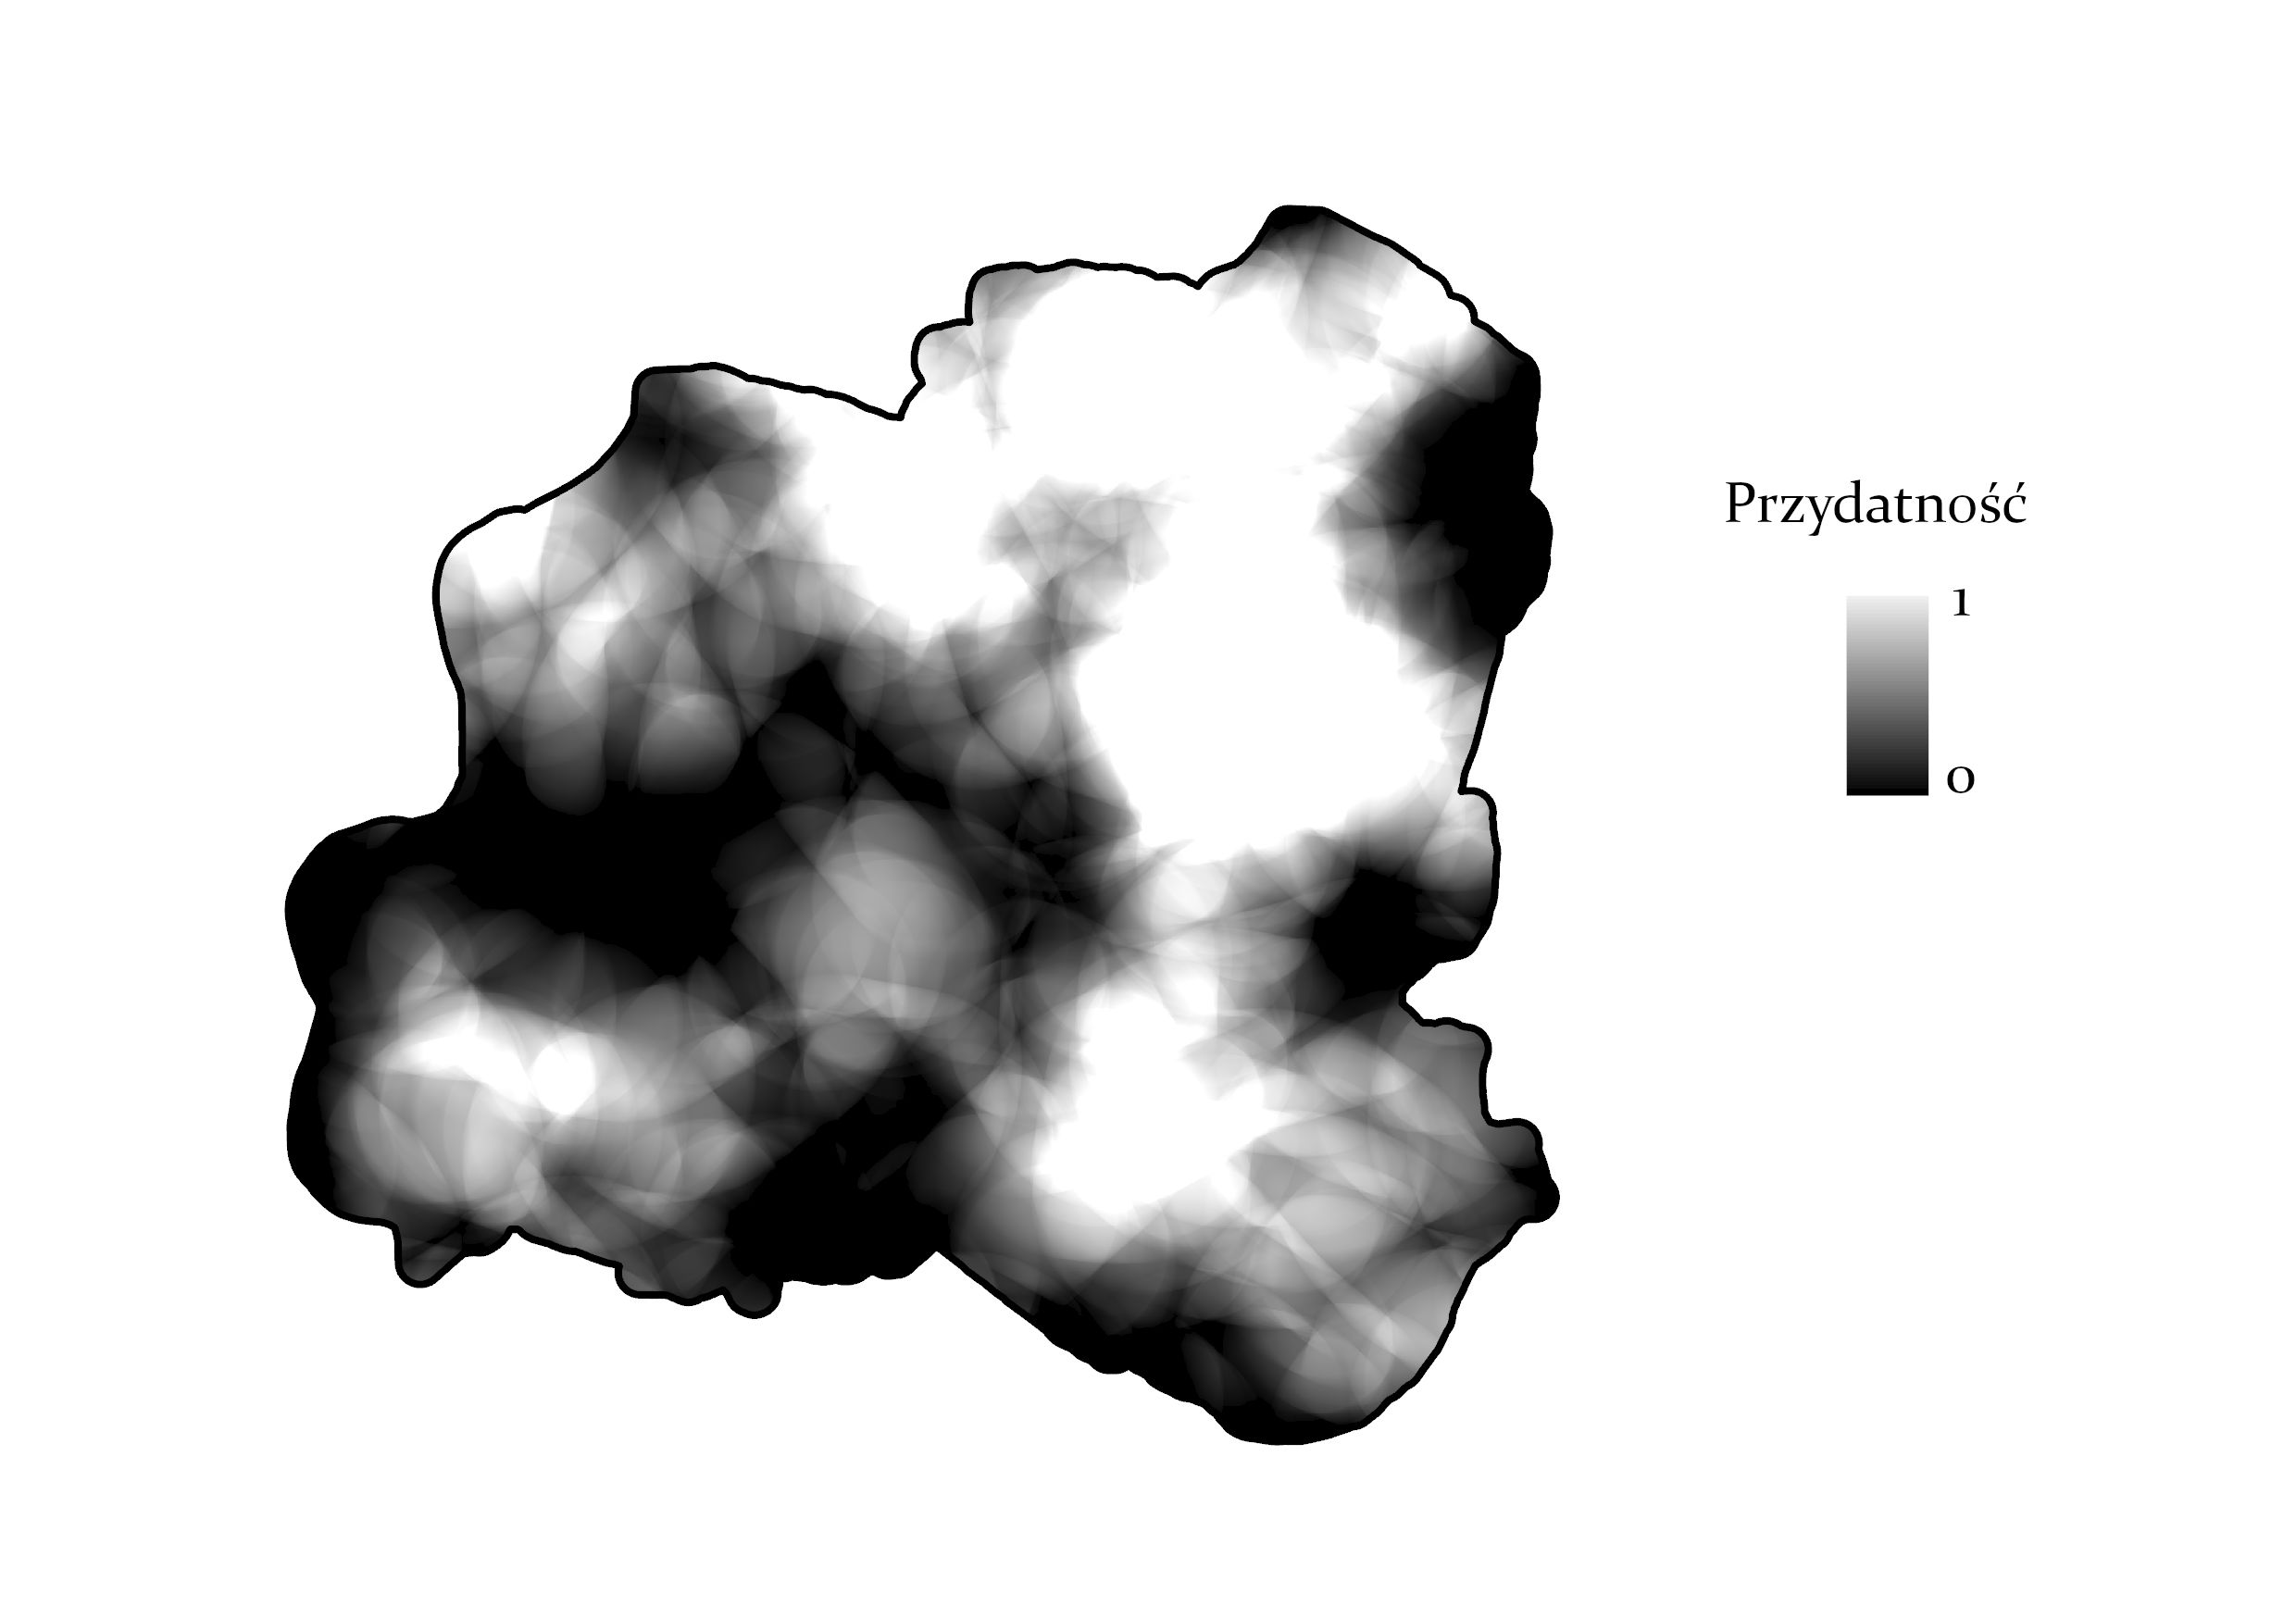
\includegraphics[width=0.75\textwidth]{img/plesna-kryterium4-layout.jpg}
    \caption*{Mapa przydatności dla kryterium 4.}
\end{figure}

\begin{figure}[H]
    \centering
    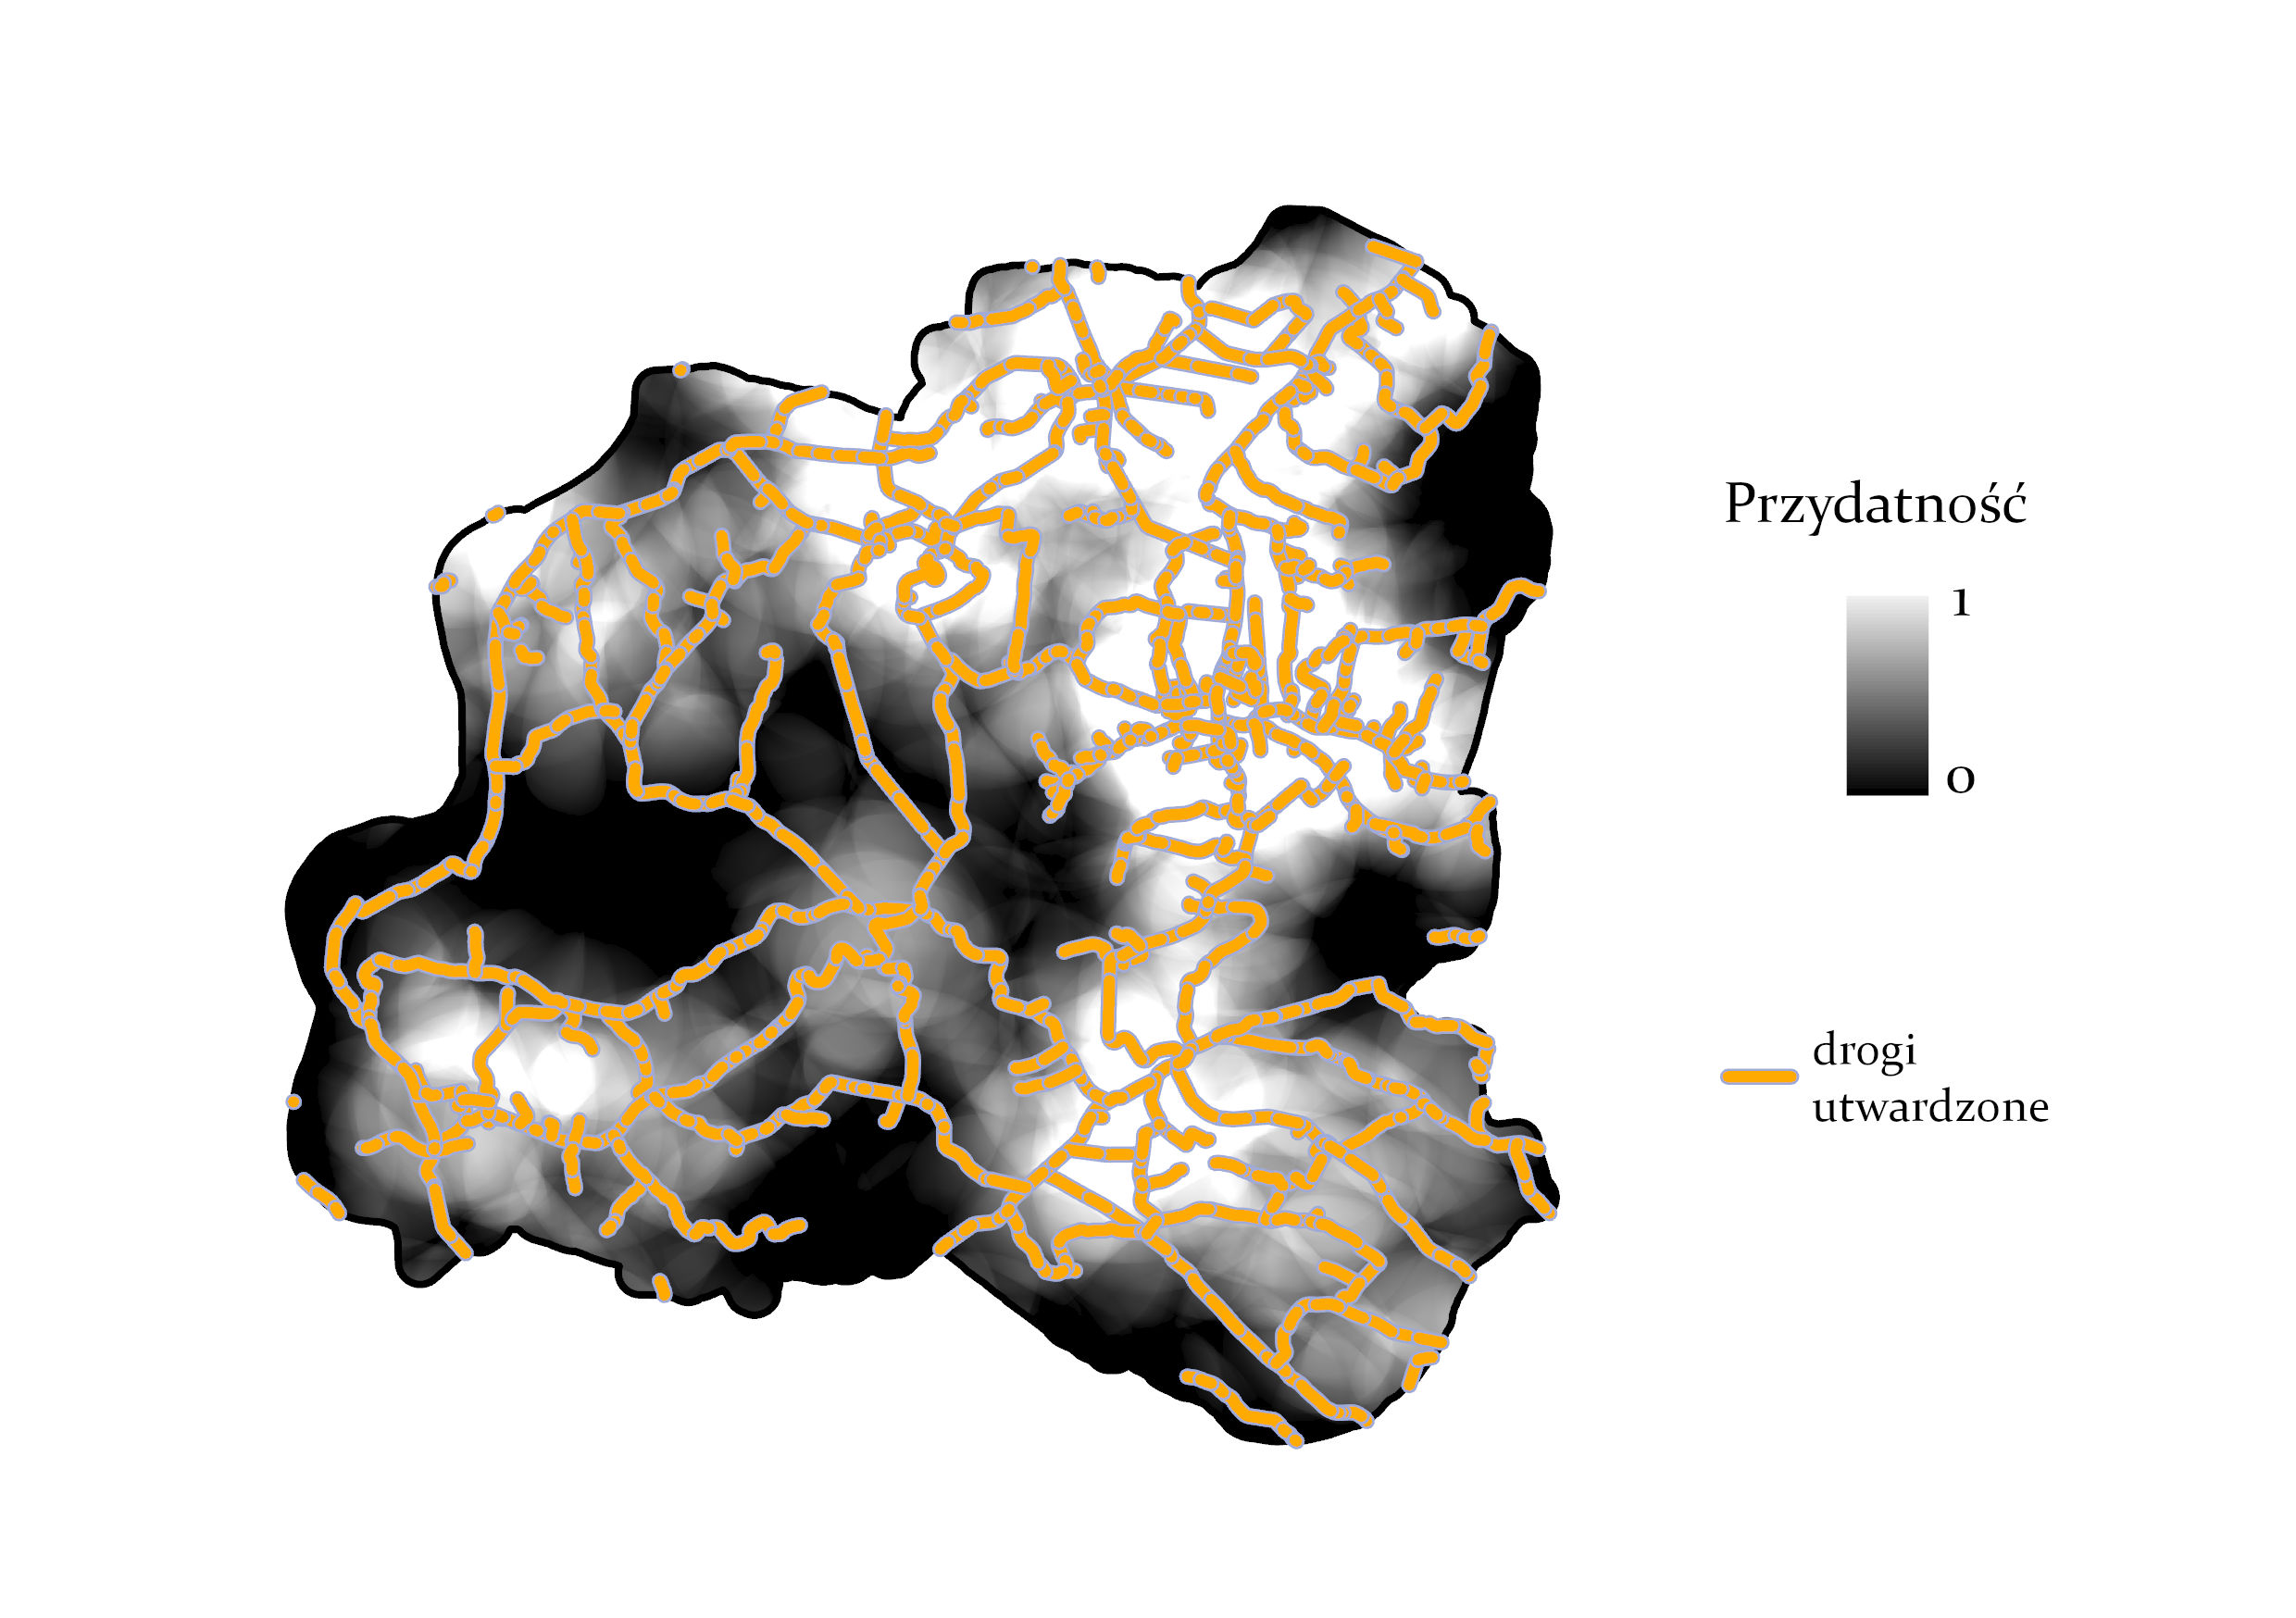
\includegraphics[width=0.75\textwidth]{img/plesna-kryterium4-drogi.jpg}
    \caption*{Mapa przydatności dla kryterium 4. zawierająca drogi utwardzone}
\end{figure}

\subsection{Kryterium 5: nachylenie stoków}

\begin{figure}[H]
    \centering
    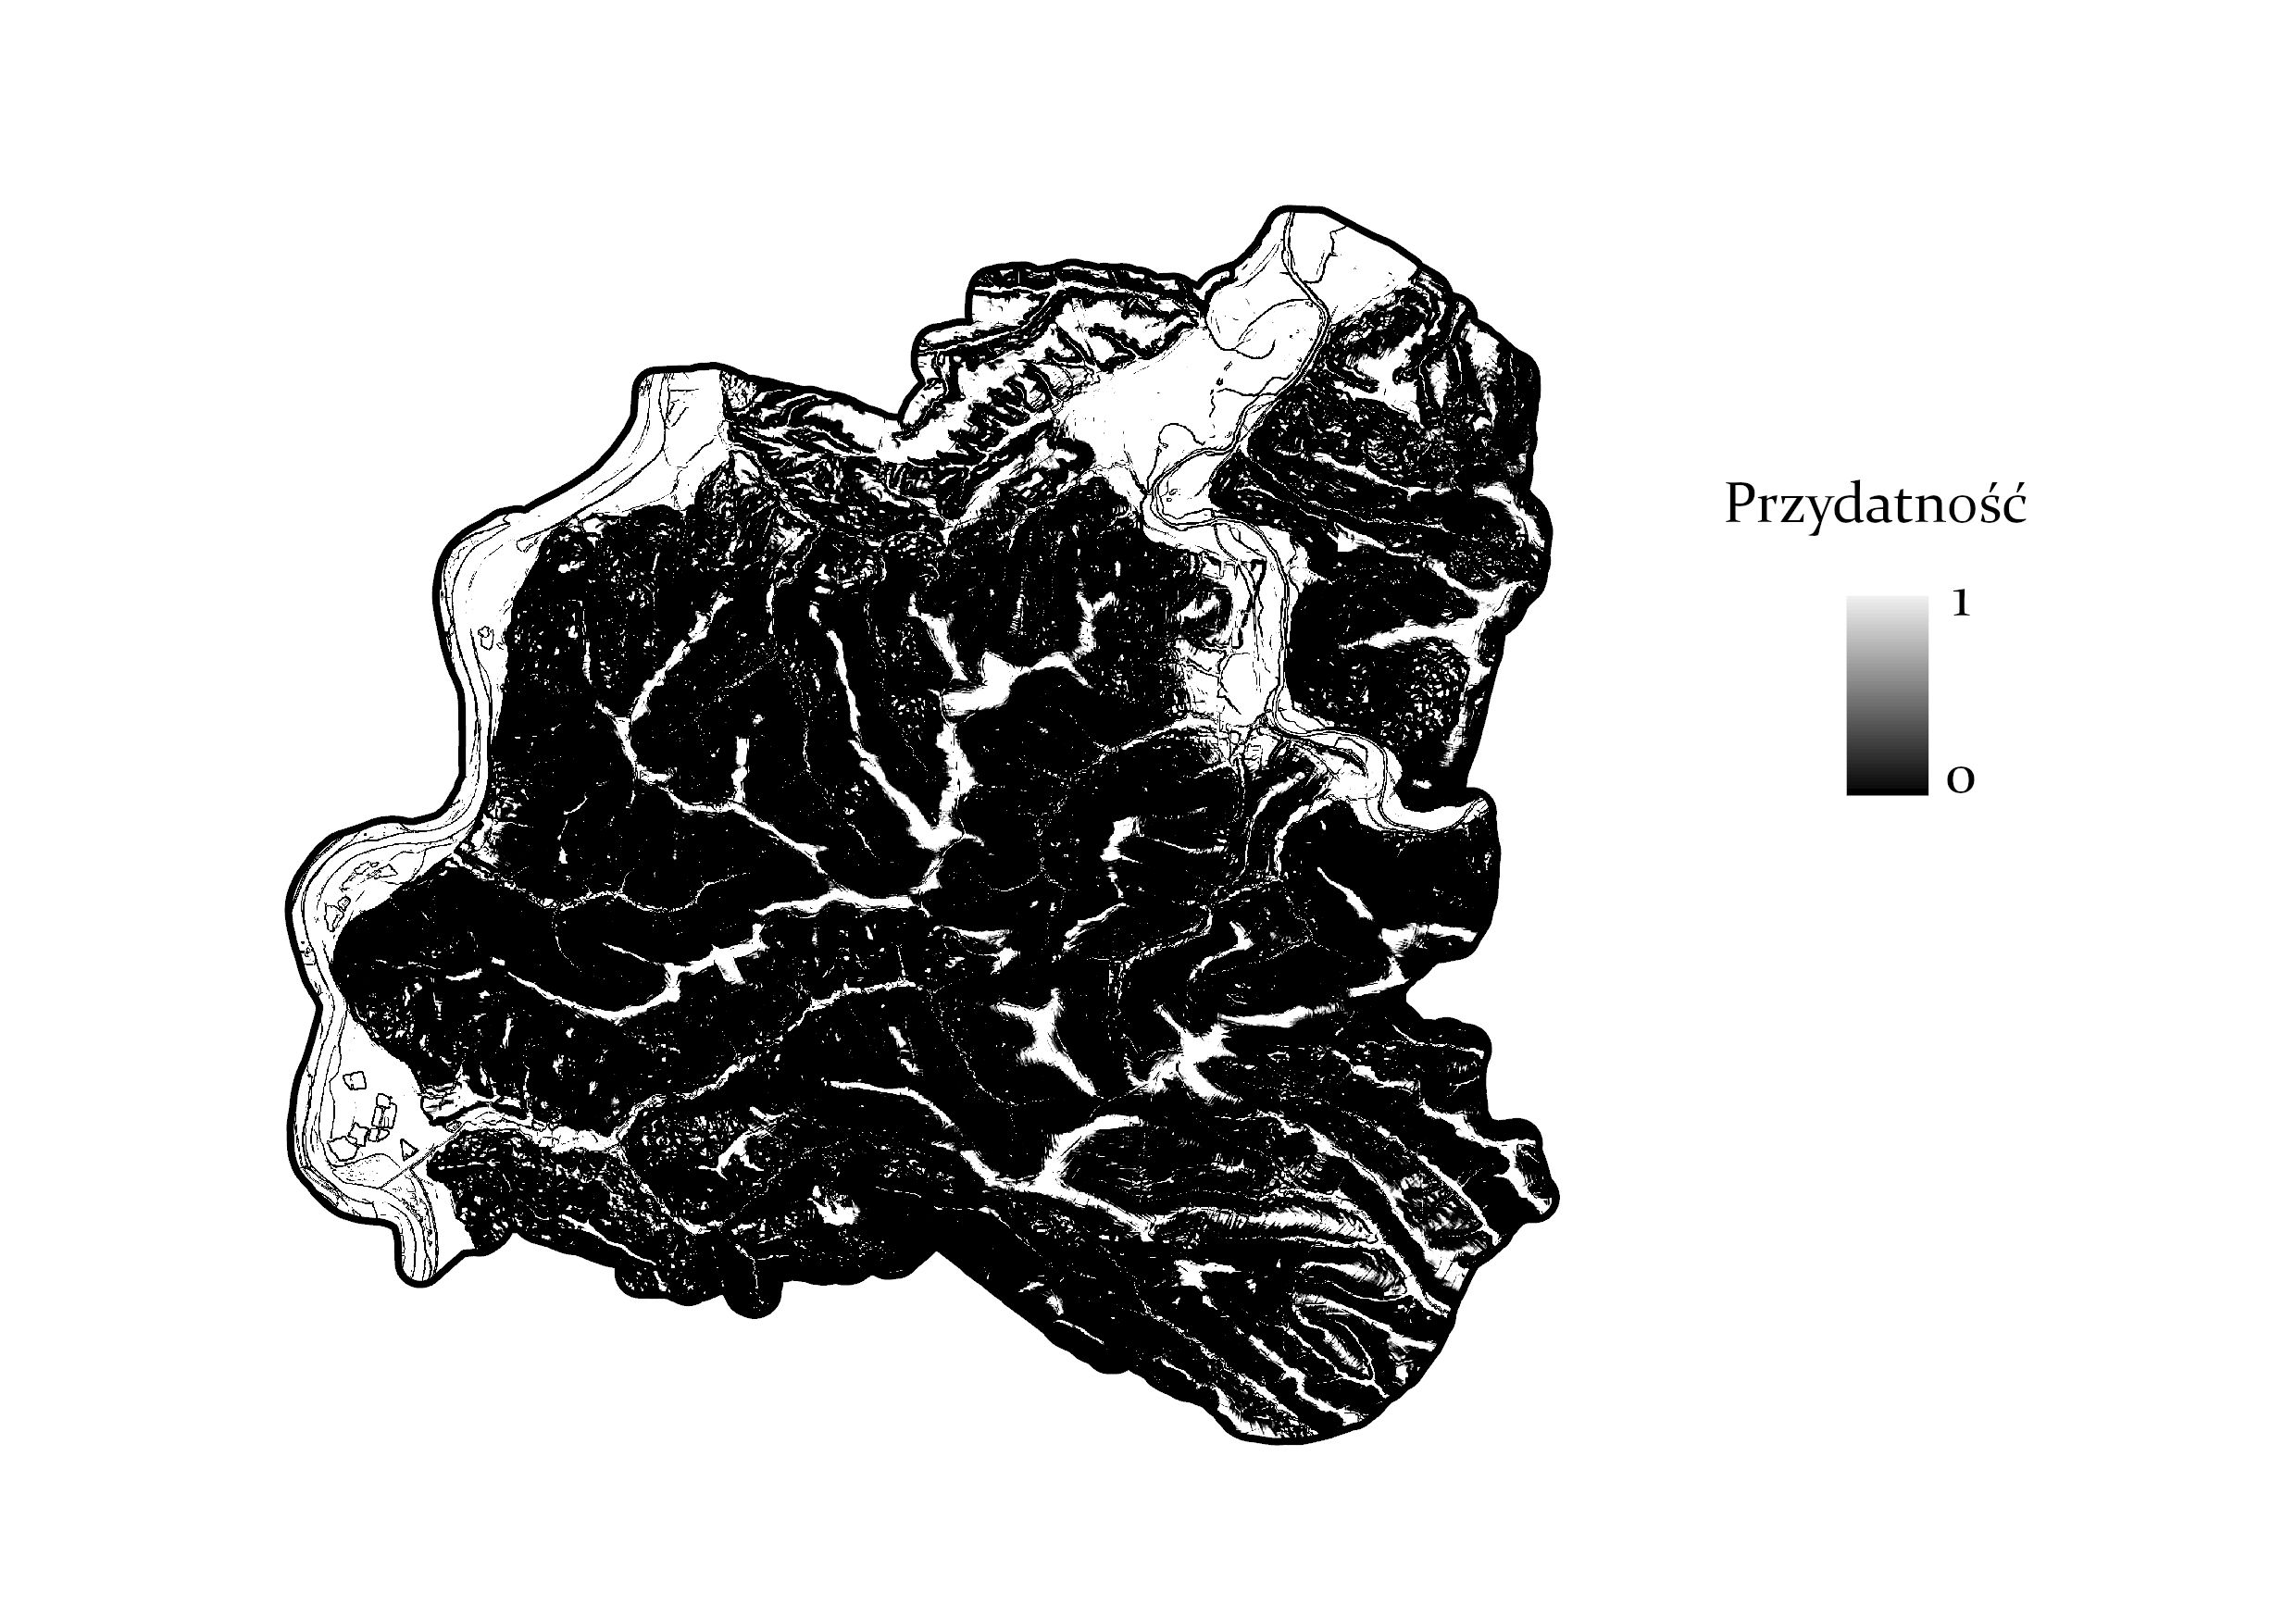
\includegraphics[width=0.75\textwidth]{img/plesna-kryterium5-layout.jpg}
    \caption*{Mapa przydatności dla kryterium 5.}
\end{figure}

\begin{figure}[H]
    \centering
    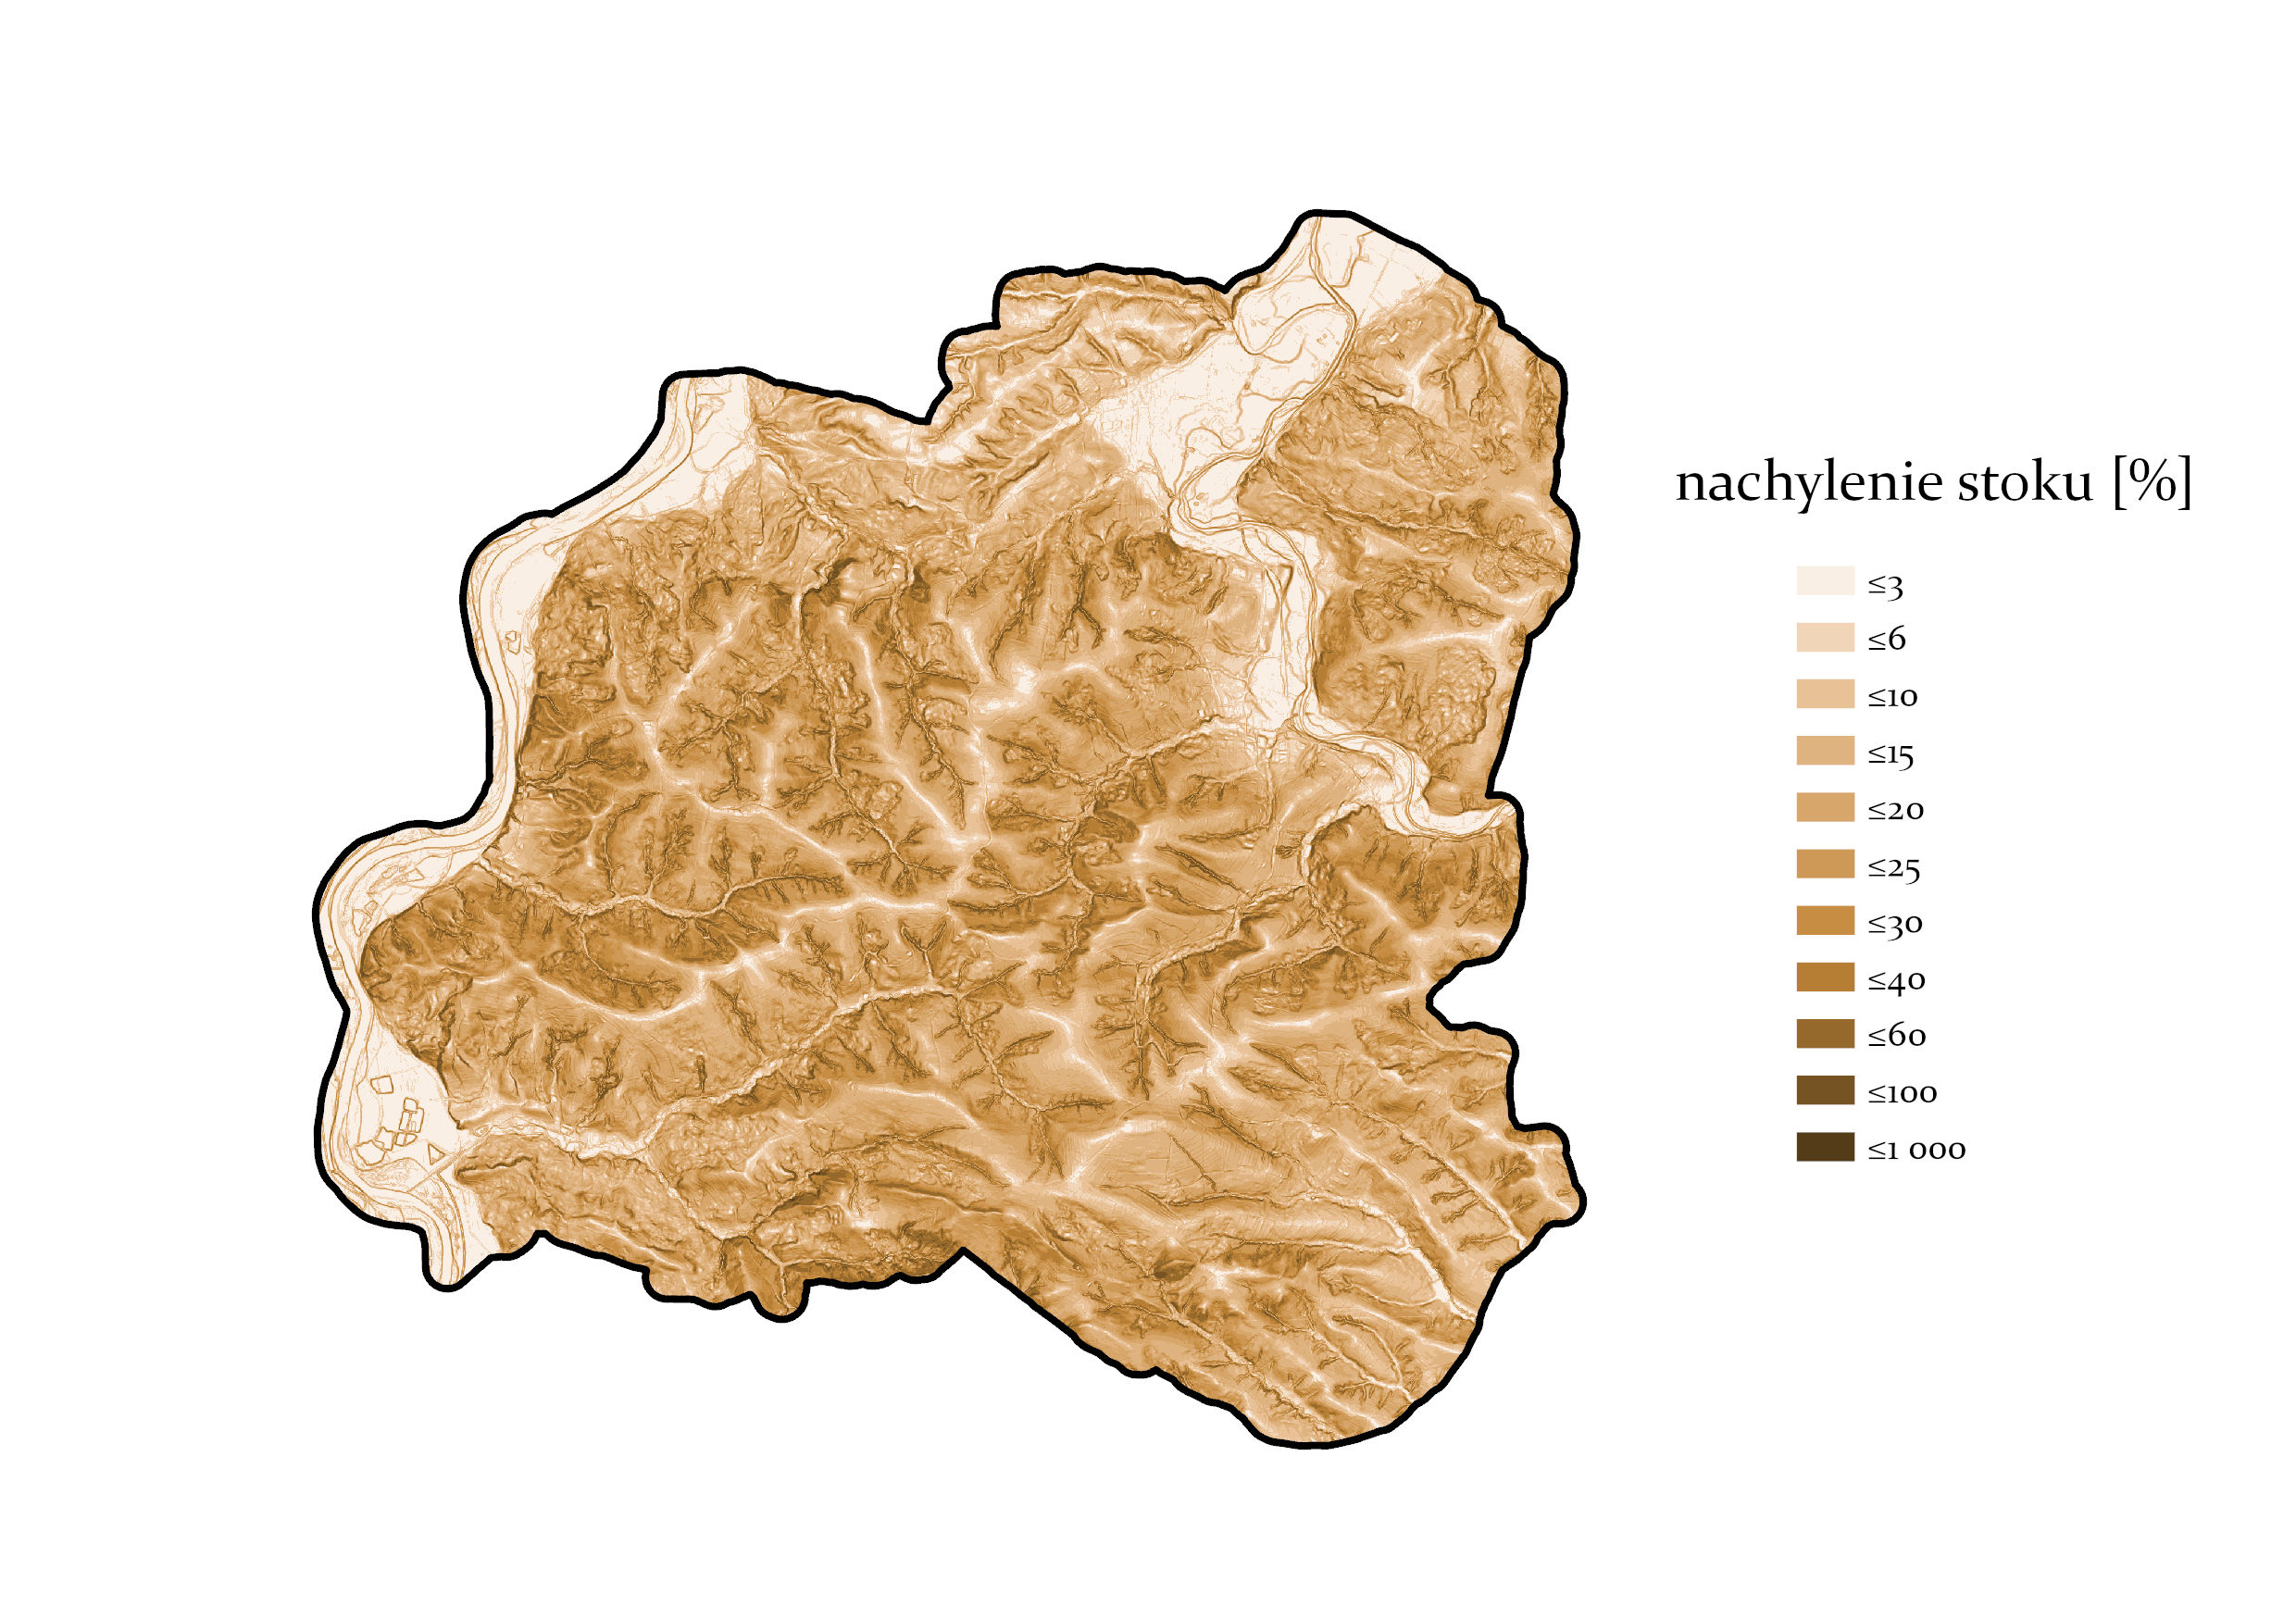
\includegraphics[width=0.75\textwidth]{img/plesna-kryterium5-stoki.jpg}
    \caption*{Mapa nachyleń stoków wykorzystana podczas sprawdzania kryterium 5.}
\end{figure}


\subsection{Kryterium 6: dostęp do światła słonecznego}
\begin{figure}[H]
    \centering
    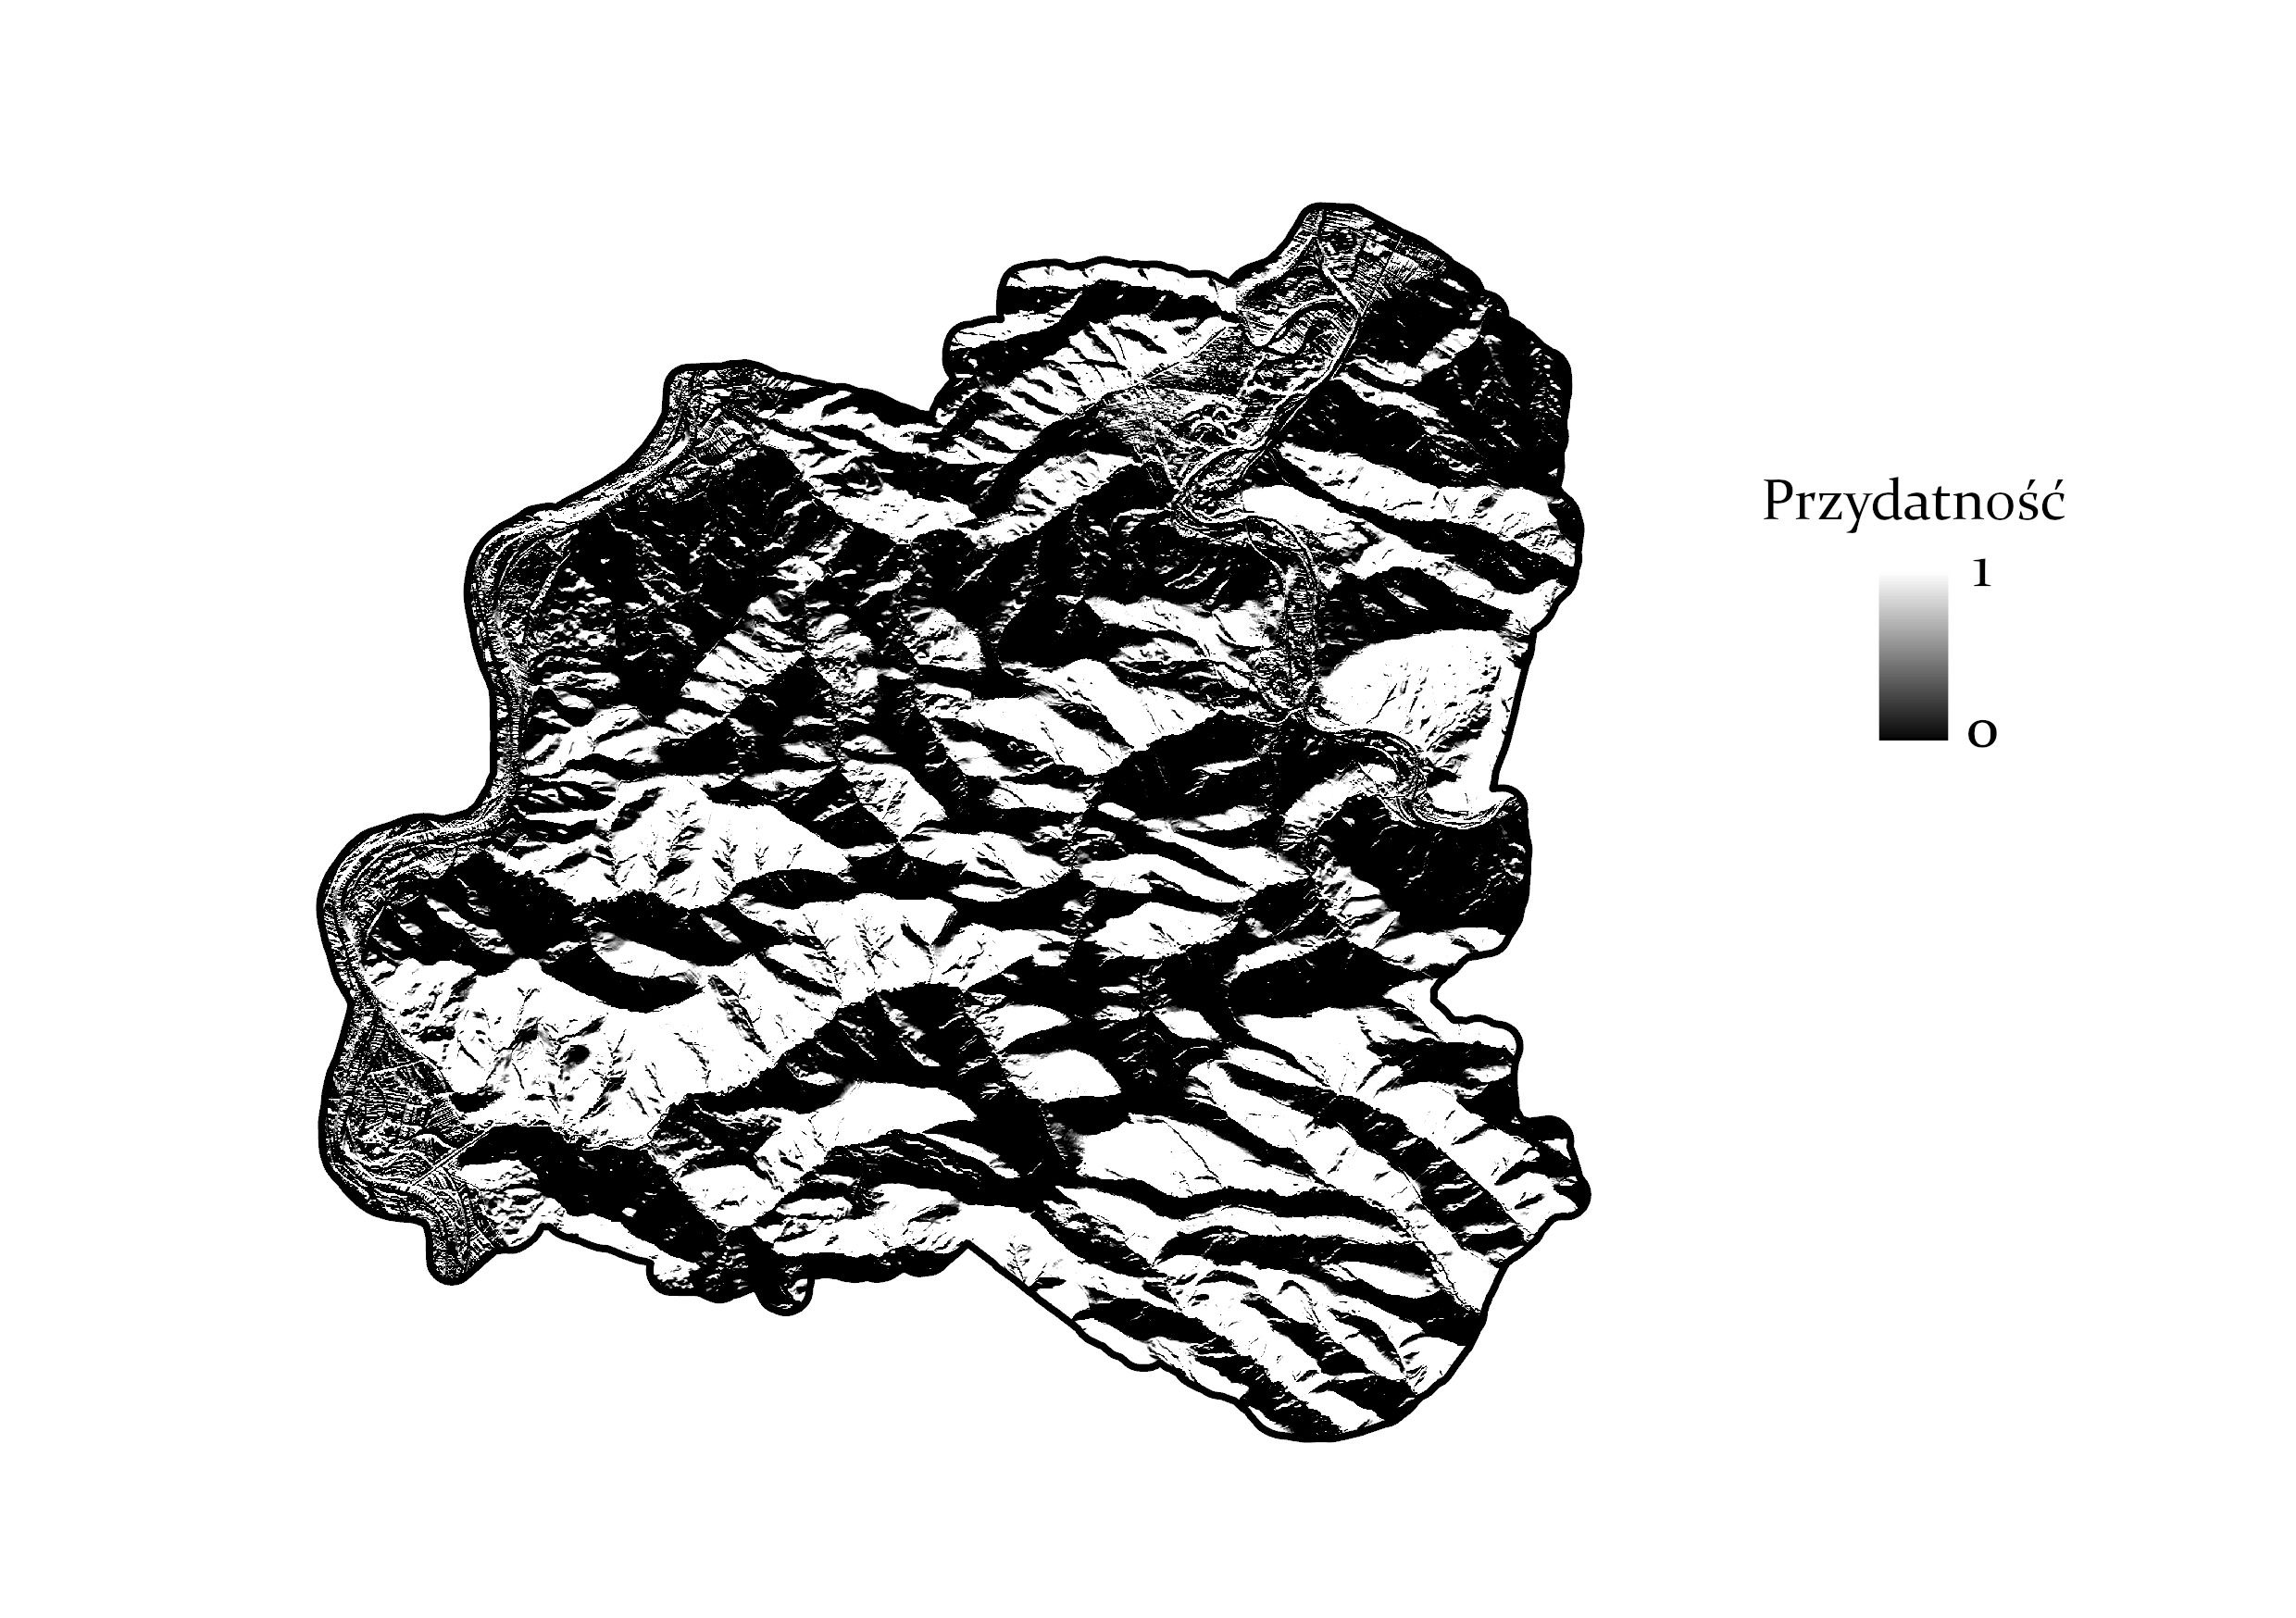
\includegraphics[width=0.75\textwidth]{img/plesna-kryterium6-layout.jpg}
    \caption*{Mapa przydatności dla kryterium 6.}
\end{figure}

\begin{figure}[H]
    \centering
    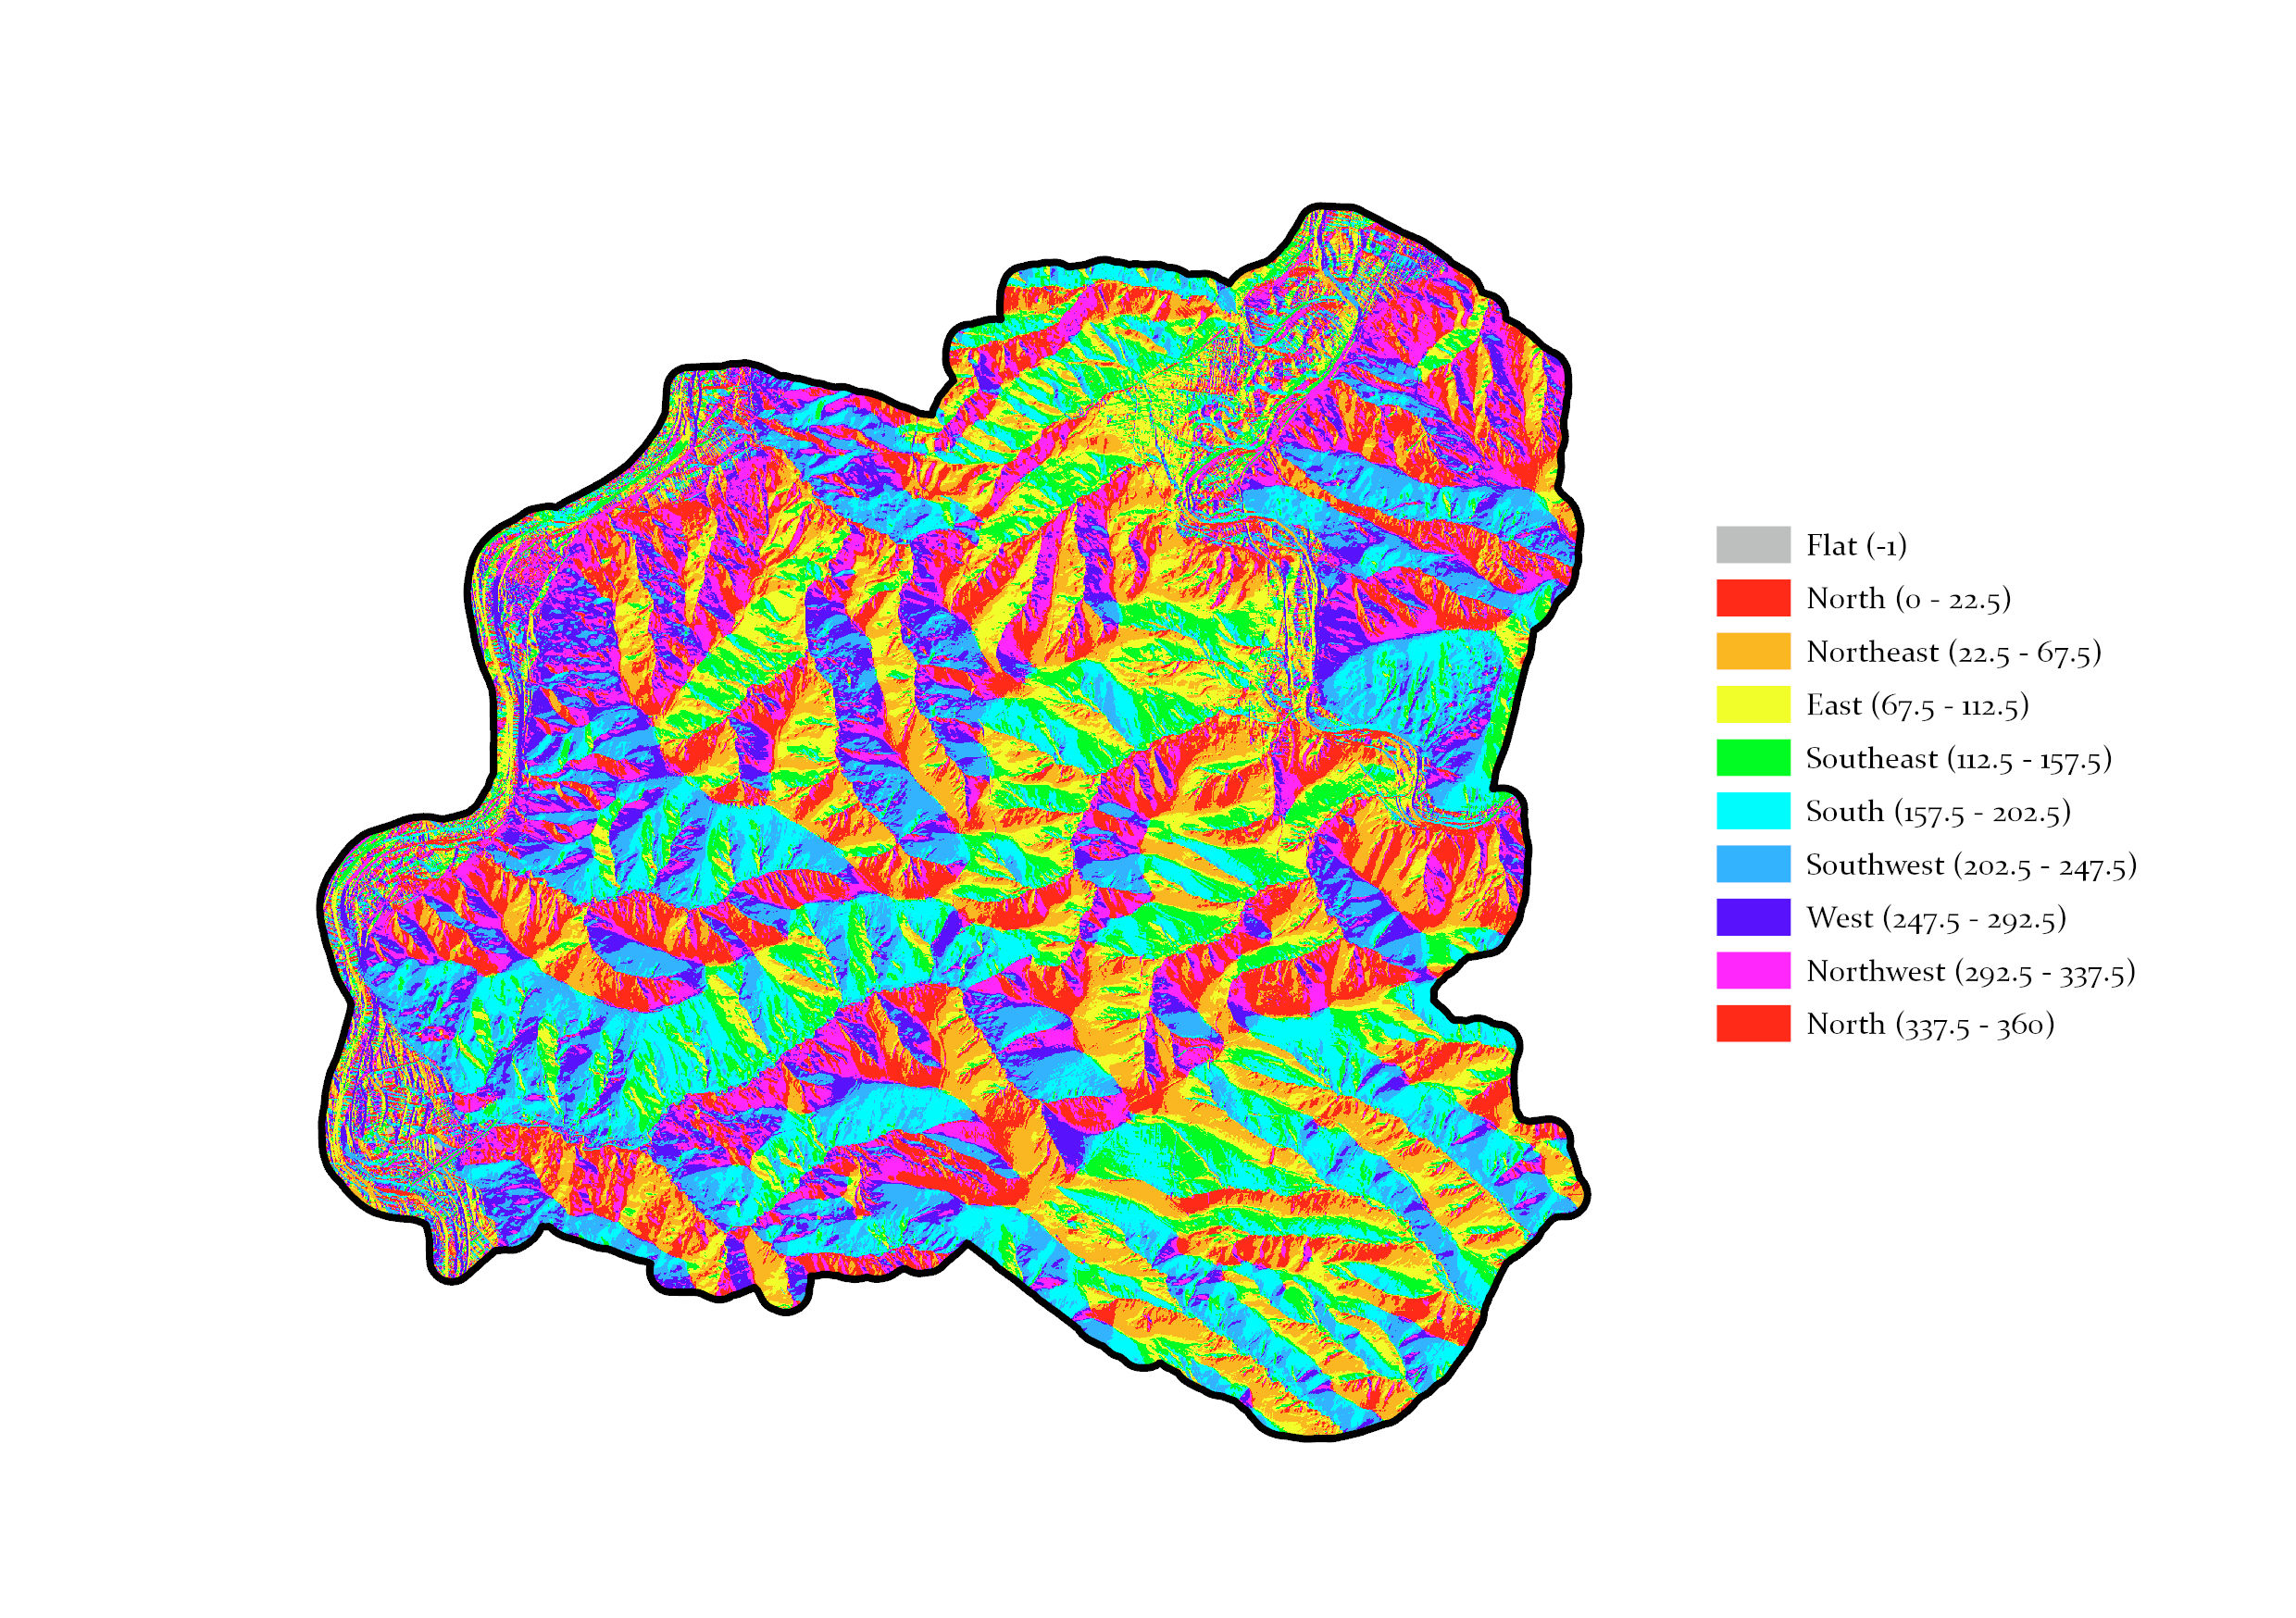
\includegraphics[width=0.75\textwidth]{img/plesna-kryterium6-aspect.jpg}
    \caption*{Mapa przydatności dla kryterium 6. zawierająca stopień wystawy słonecznej}
\end{figure}

\subsection{Kryterium 7: dojazd do istotnych drogowych węzłów komunikacyjnych}

\begin{figure}[H]
    \centering
    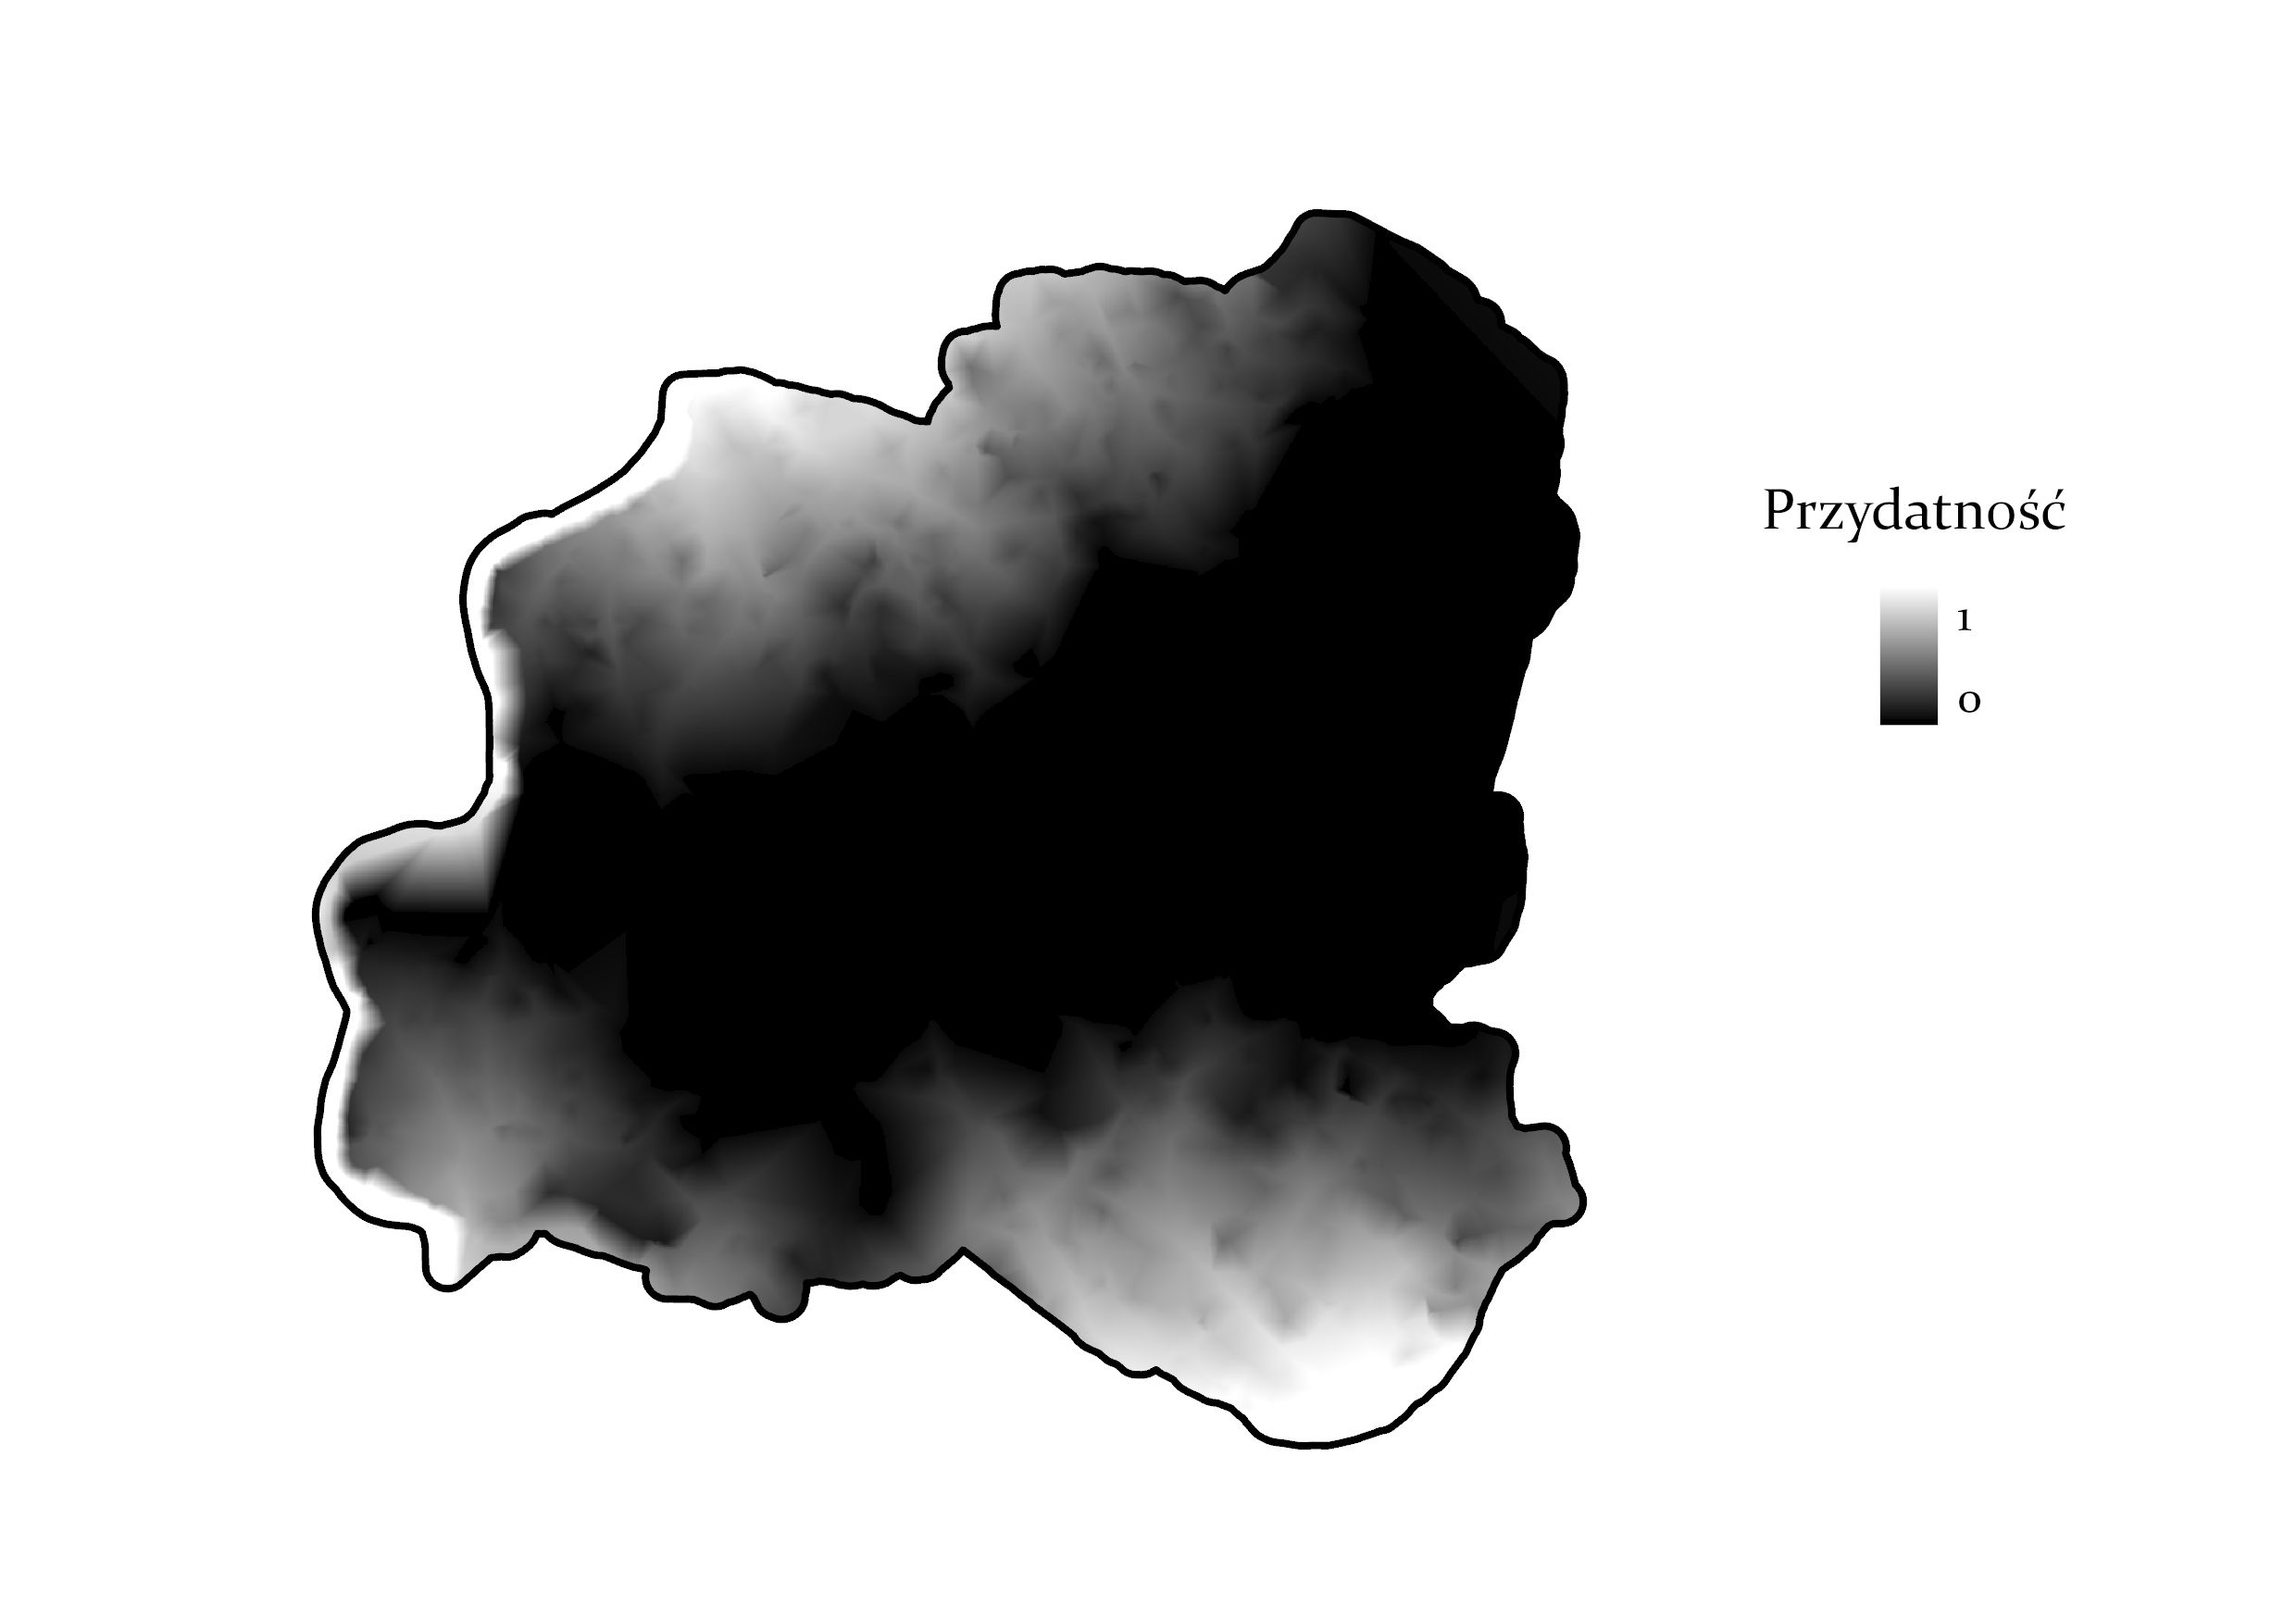
\includegraphics[width=0.75\textwidth]{img/plesna-kryterium7-layout.jpg}
    \caption*{Mapa przydatności dla kryterium 7.}
\end{figure}

\begin{figure}[H]
    \centering
    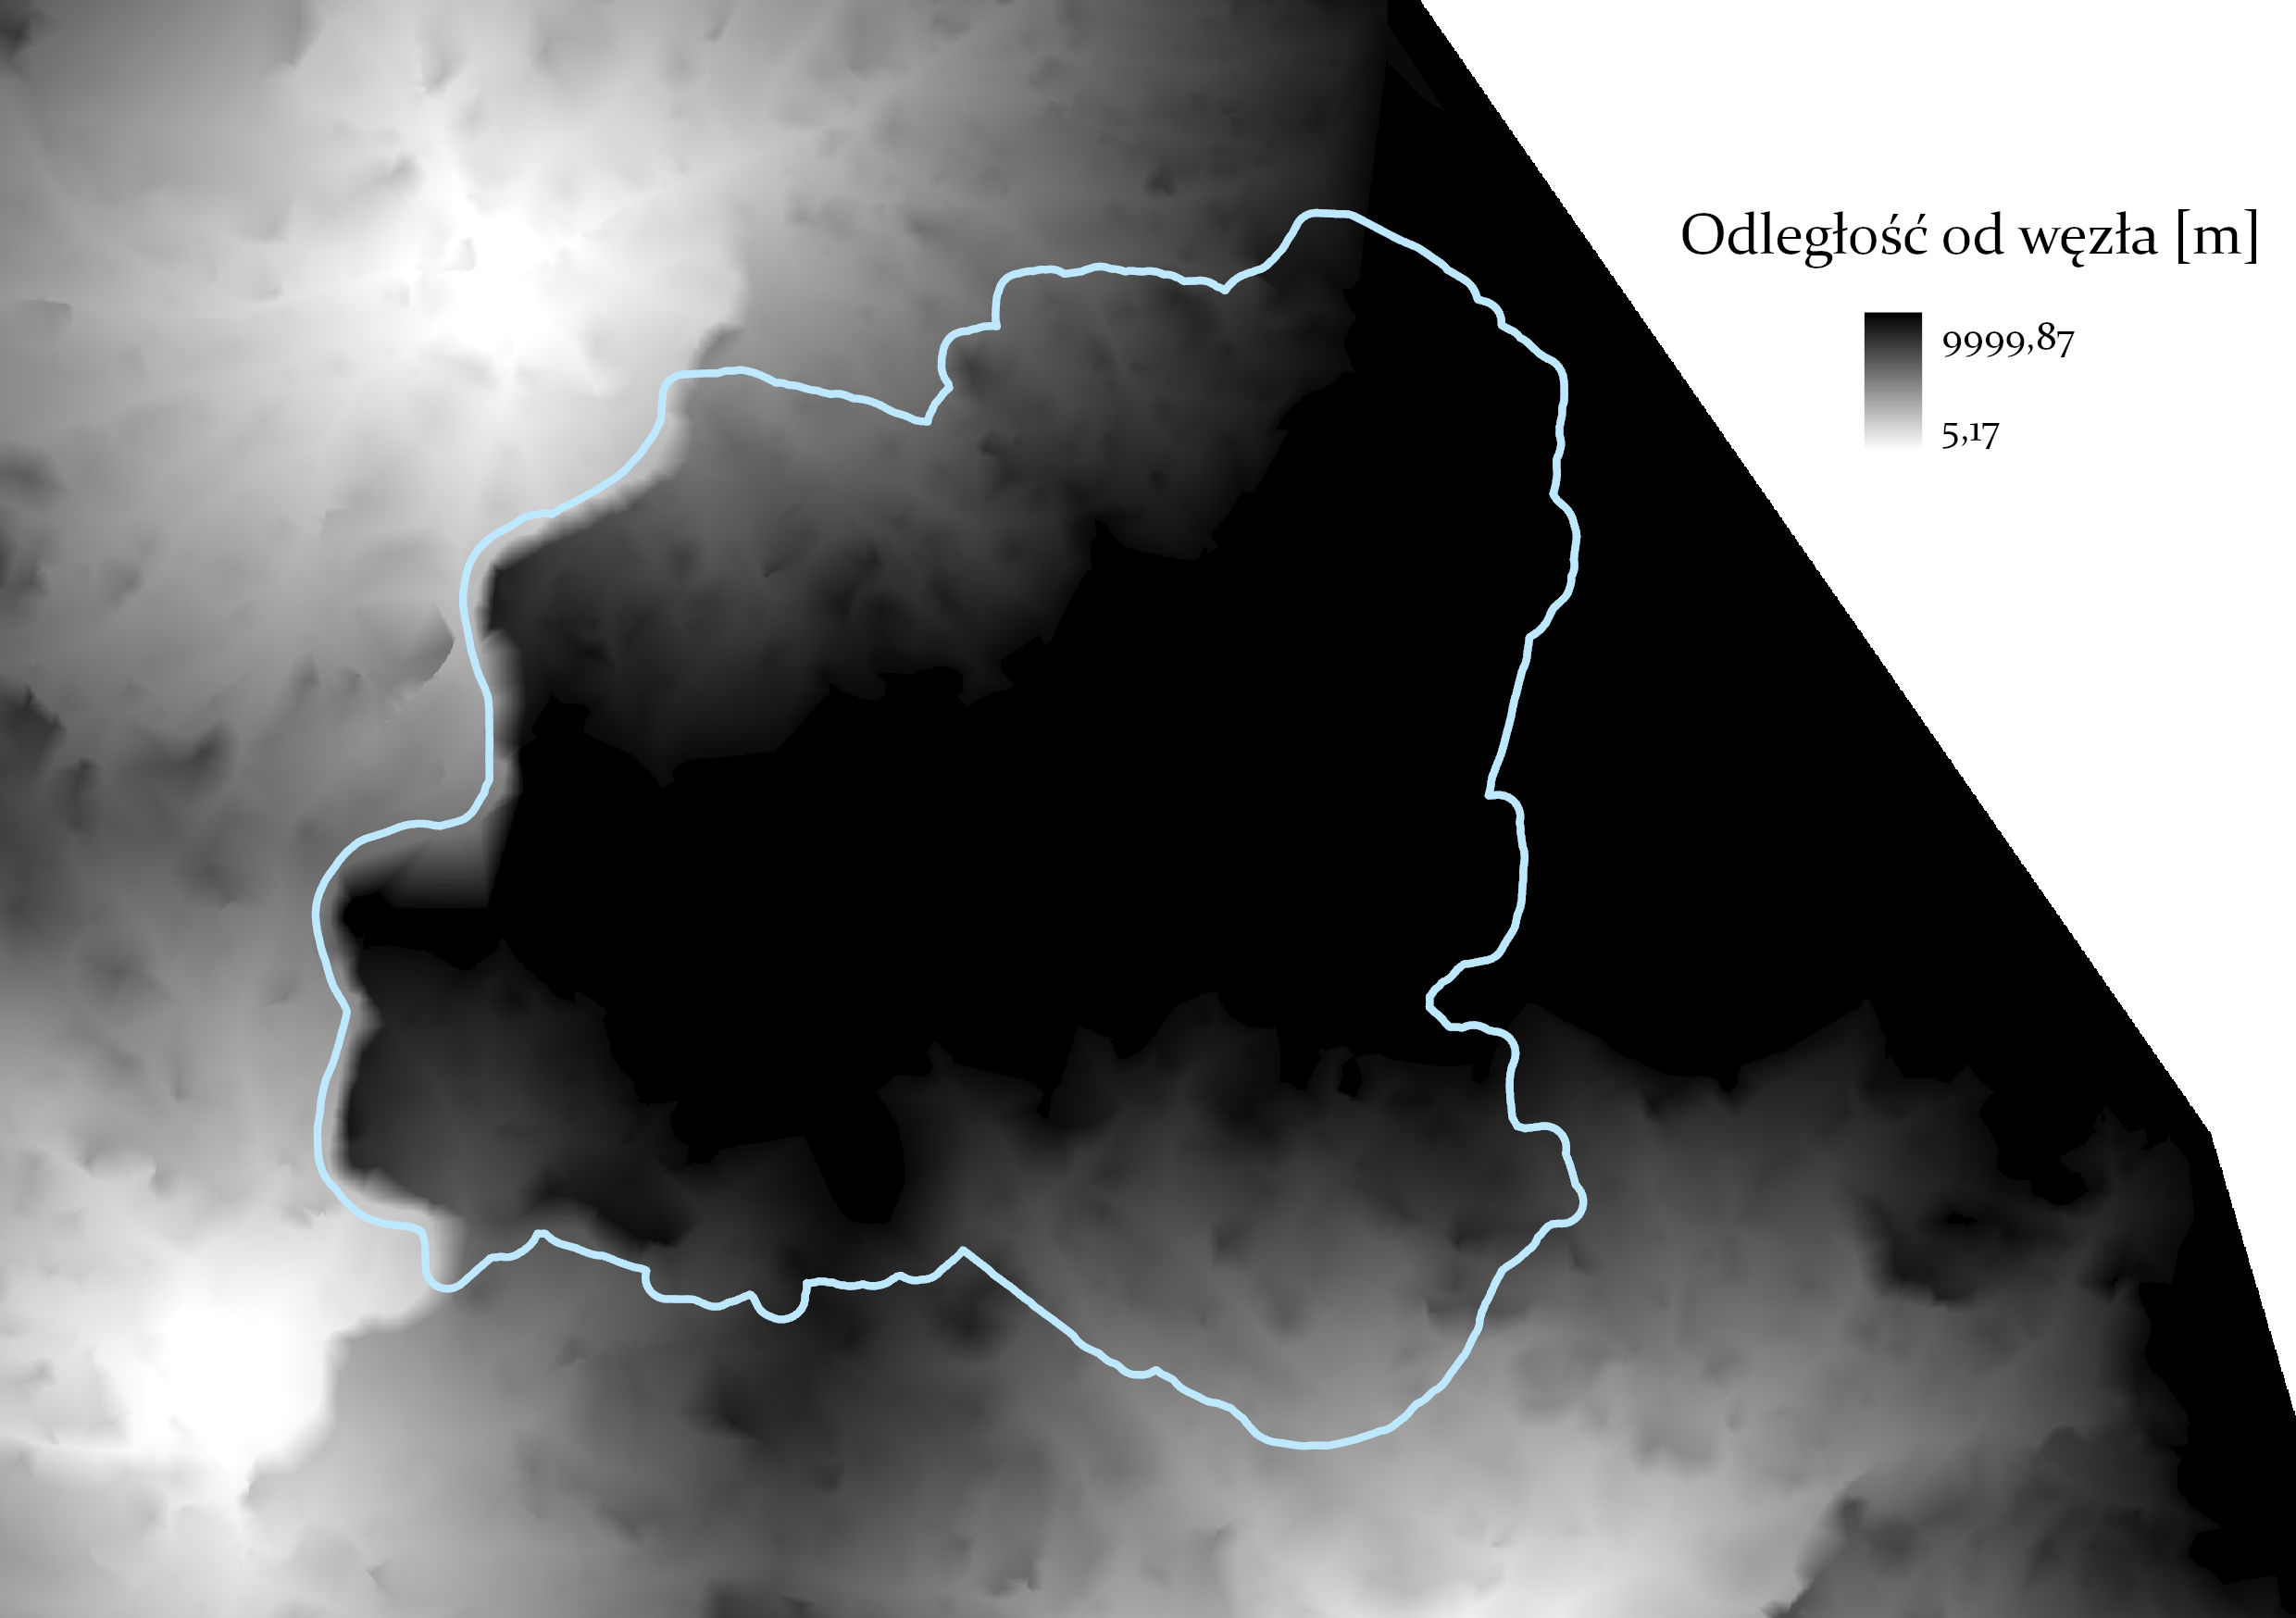
\includegraphics[width=0.75\textwidth]{img/plesna-kryterium7-wezly.jpg}
    \caption*{Mapa odległości od węzłów}
\end{figure}

\subsection{Ocena przydatności terenu}
\begin{figure}[H]
    \centering
    \includegraphics[width=0.75\textwidth]{img/plesna-rozmyte-layout.jpg}
    \caption*{Suma kryteriów rozmytych}
\end{figure}

\begin{figure}[H]
    \centering
    \includegraphics[width=0.75\textwidth]{img/plesna-ostre-layout.jpg}
    \caption*{Suma kryteriów ostrych}
\end{figure}

\begin{figure}[H]
    \centering
    \includegraphics[width=0.75\textwidth]{img/plesna-wynik.jpg}
    \caption*{Wynik łączenia kryteriów ostrych i rozmytych}
\end{figure}

\begin{figure}[H]
    \centering
    \includegraphics[width=0.75\textwidth]{img/plesna-wynik-po-reklasyfikacji.jpg}
    \caption*{Wynik łączenia kryteriów ostrych i rozmytych po reklasyfikacji}
\end{figure}

\subsection{Wybór przydatnych działek}

\begin{figure}[H]
    \centering
    \includegraphics[width=0.75\textwidth]{img/plesna-przydatne-dzialki.jpg}
    \caption*{Mapa przedstawiająca przydatne działki}
\end{figure}

\begin{figure}[H]
    \centering
    \includegraphics[width=0.75\textwidth]{img/plesna-dzialki-przydatne-ortofoto.jpg}
    \caption*{Mapa przedstawiająca przydatne działki na ortofotomapie}
\end{figure}

\begin{figure}[H]
    \centering
    \includegraphics[width=0.75\textwidth]{img/plesna-dzialki-przydatne-ortofoto-2.jpg}
    \caption*{Mapa przedstawiająca przydatne działki na ortofotomapie}
\end{figure}

\subsection{Przyłącze do sieci SN}
\begin{figure}[H]
    \centering
    \includegraphics[width=0.75\textwidth]{img/plesna-cost-raster.jpg}
    \caption*{Mapa kosztów względnych}
\end{figure}

\begin{figure}[H]
    \centering
    \includegraphics[width=0.75\textwidth]{img/plesna-cost-backlink.jpg}
    \caption*{Mapa kierunków (backlink)}
\end{figure}

\begin{figure}[H]
    \centering
    \includegraphics[width=0.75\textwidth]{img/plesna-cost-distance.jpg}
    \caption*{Mapa kosztów skumulowanych}
\end{figure}

\begin{figure}[H]
    \centering
    \includegraphics[width=0.75\textwidth]{img/plesna-dzialki-linie.jpg}
    \caption*{Mapa przedstawiająca przydatne działki oraz linie elektroenergetyczne}
\end{figure}

\end{document}